%%%%%%%%%%%%%%%%%%%%%%%%%%%%%%%%%%%%%%%%%
% The Legrand Orange Book
% LaTeX Template
% Version 2.1.1 (14/2/16)
%
% This template has been downloaded from:
% http://www.LaTeXTemplates.com
%
% Original author:
% Mathias Legrand (legrand.mathias@gmail.com) with modifications by:
% Vel (vel@latextemplates.com)
%
% License:
% CC BY-NC-SA 3.0 (http://creativecommons.org/licenses/by-nc-sa/3.0/)
%
% Compiling this template:
% This template uses biber for its bibliography and makeindex for its index.
% When you first open the template, compile it from the command line with the 
% commands below to make sure your LaTeX distribution is configured correctly:
%
% 1) pdflatex main
% 2) makeindex main.idx -s StyleInd.ist
% 3) biber main
% 4) pdflatex main x 2
%
% After this, when you wish to update the bibliography/index use the appropriate
% command above and make sure to compile with pdflatex several times 
% afterwards to propagate your changes to the document.
%
% This template also uses a number of packages which may need to be
% updated to the newest versions for the template to compile. It is strongly
% recommended you update your LaTeX distribution if you have any
% compilation errors.
%
% Important note:
% Chapter heading images should have a 2:1 width:height ratio,
% e.g. 920px width and 460px height.
%
%%%%%%%%%%%%%%%%%%%%%%%%%%%%%%%%%%%%%%%%%

%----------------------------------------------------------------------------------------
%	PACKAGES AND OTHER DOCUMENT CONFIGURATIONS
%----------------------------------------------------------------------------------------

\documentclass[12pt,fleqn]{book} % Default font size and left-justified equations

%----------------------------------------------------------------------------------------

%%%%%%%%%%%%%%%%%%%%%%%%%%%%%%%%%%%%%%%%%
% The Legrand Orange Book
% Structural Definitions File
% Version 2.0 (9/2/15)
%
% Original author:
% Mathias Legrand (legrand.mathias@gmail.com) with modifications by:
% Vel (vel@latextemplates.com)
% 
% This file has been downloaded from:
% http://www.LaTeXTemplates.com
%
% License:
% CC BY-NC-SA 3.0 (http://creativecommons.org/licenses/by-nc-sa/3.0/)
%
%%%%%%%%%%%%%%%%%%%%%%%%%%%%%%%%%%%%%%%%%

%----------------------------------------------------------------------------------------
%	VARIOUS REQUIRED PACKAGES AND CONFIGURATIONS
%----------------------------------------------------------------------------------------

\usepackage[top=3cm,bottom=3cm,left=3cm,right=3cm,headsep=10pt,a4paper]{geometry} % Page margins

\usepackage{graphicx} % Required for including pictures
\graphicspath{{Pictures/}} % Specifies the directory where pictures are stored

\usepackage{lipsum} % Inserts dummy text

\usepackage{tikz} % Required for drawing custom shapes

\usepackage[english]{babel} % English language/hyphenation

\usepackage{enumitem} % Customize lists
\setlist{nolistsep} % Reduce spacing between bullet points and numbered lists

\usepackage{booktabs} % Required for nicer horizontal rules in tables

\usepackage[table]{xcolor}

\usepackage{xcolor} % Required for specifying colors by name
\definecolor{ocre}{RGB}{31,94,219} % Define the orange color used for highlighting throughout the book

%----------------------------------------------------------------------------------------
%	FONTS
%----------------------------------------------------------------------------------------

\usepackage{avant} % Use the Avantgarde font for headings
%\usepackage{times} % Use the Times font for headings
\usepackage{mathptmx} % Use the Adobe Times Roman as the default text font together with math symbols from the Sym­bol, Chancery and Com­puter Modern fonts

\usepackage{microtype} % Slightly tweak font spacing for aesthetics
\usepackage[utf8]{inputenc} % Required for including letters with accents
\usepackage[T1]{fontenc} % Use 8-bit encoding that has 256 glyphs

%----------------------------------------------------------------------------------------
%	BIBLIOGRAPHY AND INDEX
%----------------------------------------------------------------------------------------

\usepackage{csquotes}
\usepackage[style=alphabetic,citestyle=numeric,sorting=nyt,sortcites=true,autopunct=true,autolang=hyphen,hyperref=true,abbreviate=false,backref=true,backend=biber,defernumbers=true]{biblatex}
\addbibresource{bibliography.bib} % BibTeX bibliography file
\defbibheading{bibempty}{}

\usepackage{calc} % For simpler calculation - used for spacing the index letter headings correctly
\usepackage{makeidx} % Required to make an index
\makeindex % Tells LaTeX to create the files required for indexing

%----------------------------------------------------------------------------------------
%	MAIN TABLE OF CONTENTS
%----------------------------------------------------------------------------------------

\usepackage{titletoc} % Required for manipulating the table of contents

\contentsmargin{0cm} % Removes the default margin

% Part text styling
\titlecontents{part}[0cm]
{\addvspace{20pt}\centering\large\bfseries}
{}
{}
{}

% Chapter text styling
\titlecontents{chapter}[1.25cm] % Indentation
{\addvspace{12pt}\large\sffamily\bfseries} % Spacing and font options for chapters
{\color{ocre!60}\contentslabel[\Large\thecontentslabel]{1.25cm}\color{ocre}} % Chapter number
{\color{ocre}}  
{\color{ocre!60}\normalsize\;\titlerule*[.5pc]{.}\;\thecontentspage} % Page number

% Section text styling
\titlecontents{section}[1.25cm] % Indentation
{\addvspace{3pt}\sffamily\bfseries} % Spacing and font options for sections
{\contentslabel[\thecontentslabel]{1.25cm}} % Section number
{}
{\hfill\color{black}\thecontentspage} % Page number
[]

% Subsection text styling
\titlecontents{subsection}[1.25cm] % Indentation
{\addvspace{1pt}\sffamily\small} % Spacing and font options for subsections
{\contentslabel[\thecontentslabel]{1.25cm}} % Subsection number
{}
{\ \titlerule*[.5pc]{.}\;\thecontentspage} % Page number
[]

% List of figures
\titlecontents{figure}[0em]
{\addvspace{-5pt}\sffamily}
{\thecontentslabel\hspace*{1em}}
{}
{\ \titlerule*[.5pc]{.}\;\thecontentspage}
[]

% List of tables
\titlecontents{table}[0em]
{\addvspace{-5pt}\sffamily}
{\thecontentslabel\hspace*{1em}}
{}
{\ \titlerule*[.5pc]{.}\;\thecontentspage}
[]

%----------------------------------------------------------------------------------------
%	MINI TABLE OF CONTENTS IN PART HEADS
%----------------------------------------------------------------------------------------

% Chapter text styling
\titlecontents{lchapter}[0em] % Indenting
{\addvspace{15pt}\large\sffamily\bfseries} % Spacing and font options for chapters
{\color{ocre}\contentslabel[\Large\thecontentslabel]{1.25cm}\color{ocre}} % Chapter number
{}  
{\color{ocre}\normalsize\sffamily\bfseries\;\titlerule*[.5pc]{.}\;\thecontentspage} % Page number

% Section text styling
\titlecontents{lsection}[0em] % Indenting
{\sffamily\small} % Spacing and font options for sections
{\contentslabel[\thecontentslabel]{1.25cm}} % Section number
{}
{}

% Subsection text styling
\titlecontents{lsubsection}[.5em] % Indentation
{\normalfont\footnotesize\sffamily} % Font settings
{}
{}
{}

%----------------------------------------------------------------------------------------
%	PAGE HEADERS
%----------------------------------------------------------------------------------------

\usepackage{fancyhdr} % Required for header and footer configuration

\pagestyle{fancy}
\renewcommand{\chaptermark}[1]{\markboth{\sffamily\normalsize\bfseries\chaptername\ \thechapter.\ #1}{}} % Chapter text font settings
\renewcommand{\sectionmark}[1]{\markright{\sffamily\normalsize\thesection\hspace{5pt}#1}{}} % Section text font settings
\fancyhf{} \fancyhead[LE,RO]{\sffamily\normalsize\thepage} % Font setting for the page number in the header
\fancyhead[LO]{\rightmark} % Print the nearest section name on the left side of odd pages
\fancyhead[RE]{\leftmark} % Print the current chapter name on the right side of even pages
\renewcommand{\headrulewidth}{0.5pt} % Width of the rule under the header
\addtolength{\headheight}{2.5pt} % Increase the spacing around the header slightly
\renewcommand{\footrulewidth}{0pt} % Removes the rule in the footer
\fancypagestyle{plain}{\fancyhead{}\renewcommand{\headrulewidth}{0pt}} % Style for when a plain pagestyle is specified

% Removes the header from odd empty pages at the end of chapters
\makeatletter
\renewcommand{\cleardoublepage}{
\clearpage\ifodd\c@page\else
\hbox{}
\vspace*{\fill}
\thispagestyle{empty}
\newpage
\fi}

%----------------------------------------------------------------------------------------
%	THEOREM STYLES
%----------------------------------------------------------------------------------------

\usepackage{amsmath,amsfonts,amssymb,amsthm} % For math equations, theorems, symbols, etc

\newcommand{\intoo}[2]{\mathopen{]}#1\,;#2\mathclose{[}}
\newcommand{\ud}{\mathop{\mathrm{{}d}}\mathopen{}}
\newcommand{\intff}[2]{\mathopen{[}#1\,;#2\mathclose{]}}
\newtheorem{notation}{Notation}[chapter]

% Boxed/framed environments
\newtheoremstyle{ocrenumbox}% % Theorem style name
{0pt}% Space above
{0pt}% Space below
{\normalfont}% % Body font
{}% Indent amount
{\small\bf\sffamily\color{ocre}}% % Theorem head font
{\;}% Punctuation after theorem head
{0.25em}% Space after theorem head
{\small\sffamily\color{ocre}\thmname{#1}\nobreakspace\thmnumber{\@ifnotempty{#1}{}\@upn{#2}}% Theorem text (e.g. Theorem 2.1)
\thmnote{\nobreakspace\the\thm@notefont\sffamily\bfseries\color{black}---\nobreakspace#3.}} % Optional theorem note
\renewcommand{\qedsymbol}{$\blacksquare$}% Optional qed square

\newtheoremstyle{blacknumex}% Theorem style name
{5pt}% Space above
{5pt}% Space below
{\normalfont}% Body font
{} % Indent amount
{\small\bf\sffamily}% Theorem head font
{\;}% Punctuation after theorem head
{0.25em}% Space after theorem head
{\small\sffamily{\tiny\ensuremath{\blacksquare}}\nobreakspace\thmname{#1}\nobreakspace\thmnumber{\@ifnotempty{#1}{}\@upn{#2}}% Theorem text (e.g. Theorem 2.1)
\thmnote{\nobreakspace\the\thm@notefont\sffamily\bfseries---\nobreakspace#3.}}% Optional theorem note

\newtheoremstyle{blacknumbox} % Theorem style name
{0pt}% Space above
{0pt}% Space below
{\normalfont}% Body font
{}% Indent amount
{\small\bf\sffamily}% Theorem head font
{\;}% Punctuation after theorem head
{0.25em}% Space after theorem head
{\small\sffamily\thmname{#1}\nobreakspace\thmnumber{\@ifnotempty{#1}{}\@upn{#2}}% Theorem text (e.g. Theorem 2.1)
\thmnote{\nobreakspace\the\thm@notefont\sffamily\bfseries---\nobreakspace#3.}}% Optional theorem note

% Non-boxed/non-framed environments
\newtheoremstyle{ocrenum}% % Theorem style name
{5pt}% Space above
{5pt}% Space below
{\normalfont}% % Body font
{}% Indent amount
{\small\bf\sffamily\color{ocre}}% % Theorem head font
{\;}% Punctuation after theorem head
{0.25em}% Space after theorem head
{\small\sffamily\color{ocre}\thmname{#1}\nobreakspace\thmnumber{\@ifnotempty{#1}{}\@upn{#2}}% Theorem text (e.g. Theorem 2.1)
\thmnote{\nobreakspace\the\thm@notefont\sffamily\bfseries\color{black}---\nobreakspace#3.}} % Optional theorem note
\renewcommand{\qedsymbol}{$\blacksquare$}% Optional qed square
\makeatother

% Defines the theorem text style for each type of theorem to one of the three styles above
\newcounter{dummy} 
\numberwithin{dummy}{section}
\theoremstyle{ocrenumbox}
\newtheorem{theoremeT}[dummy]{Theorem}
\newtheorem{problem}{Problem}[chapter]
\newtheorem{noteT}{Note}[chapter]
\theoremstyle{blacknumex}
\newtheorem{exampleT}{Example}[chapter]
\theoremstyle{blacknumbox}
\newtheorem{vocabulary}{Vocabulary}[chapter]
\newtheorem{definitionT}{Definition}[section]
\newtheorem{corollaryT}[dummy]{Corollary}
\theoremstyle{ocrenum}
\newtheorem{proposition}[dummy]{Proposition}

%----------------------------------------------------------------------------------------
%	DEFINITION OF COLORED BOXES
%----------------------------------------------------------------------------------------

\RequirePackage[framemethod=default]{mdframed} % Required for creating the theorem, definition, exercise and corollary boxes

% Theorem box
\newmdenv[skipabove=7pt,
skipbelow=7pt,
backgroundcolor=black!5,
linecolor=ocre,
innerleftmargin=5pt,
innerrightmargin=5pt,
innertopmargin=5pt,
leftmargin=0cm,
rightmargin=0cm,
innerbottommargin=5pt]{tBox}

% Exercise box	  
\newmdenv[skipabove=7pt,
skipbelow=7pt,
rightline=false,
leftline=true,
topline=false,
bottomline=false,
backgroundcolor=ocre!10,
linecolor=ocre,
innerleftmargin=5pt,
innerrightmargin=5pt,
innertopmargin=5pt,
innerbottommargin=5pt,
leftmargin=0cm,
rightmargin=0cm,
linewidth=4pt]{eBox}	

% Definition box
\newmdenv[skipabove=7pt,
skipbelow=7pt,
rightline=false,
leftline=true,
topline=false,
bottomline=false,
linecolor=ocre,
innerleftmargin=5pt,
innerrightmargin=5pt,
innertopmargin=0pt,
leftmargin=0cm,
rightmargin=0cm,
linewidth=4pt,
innerbottommargin=0pt]{dBox}	

% Corollary box
\newmdenv[skipabove=7pt,
skipbelow=7pt,
rightline=false,
leftline=true,
topline=false,
bottomline=false,
linecolor=gray,
backgroundcolor=black!5,
innerleftmargin=5pt,
innerrightmargin=5pt,
innertopmargin=5pt,
leftmargin=0cm,
rightmargin=0cm,
linewidth=4pt,
innerbottommargin=5pt]{cBox}

% Creates an environment for each type of theorem and assigns it a theorem text style from the "Theorem Styles" section above and a colored box from above
\newenvironment{theorem}{\begin{tBox}\begin{theoremeT}}{\end{theoremeT}\end{tBox}}
\newenvironment{note}{\begin{eBox}\begin{noteT}}{\hfill{\color{ocre}\tiny\ensuremath{\blacksquare}}\end{noteT}\end{eBox}}				  
\newenvironment{definition}{\begin{dBox}\begin{definitionT}}{\end{definitionT}\end{dBox}}	
\newenvironment{example}{\begin{exampleT}}{\hfill{\tiny\ensuremath{\blacksquare}}\end{exampleT}}		
\newenvironment{corollary}{\begin{cBox}\begin{corollaryT}}{\end{corollaryT}\end{cBox}}	

%----------------------------------------------------------------------------------------
%	REMARK ENVIRONMENT
%----------------------------------------------------------------------------------------

\newenvironment{remark}{\par\vspace{10pt}\small % Vertical white space above the remark and smaller font size
\begin{list}{}{
\leftmargin=35pt % Indentation on the left
\rightmargin=25pt}\item\ignorespaces % Indentation on the right
\makebox[-2.5pt]{\begin{tikzpicture}[overlay]
\node[draw=ocre!60,line width=1pt,circle,fill=ocre!25,font=\sffamily\bfseries,inner sep=2pt,outer sep=0pt] at (-15pt,0pt){\textcolor{ocre}{R}};\end{tikzpicture}} % Orange R in a circle
\advance\baselineskip -1pt}{\end{list}\vskip5pt} % Tighter line spacing and white space after remark

%----------------------------------------------------------------------------------------
%	SECTION NUMBERING IN THE MARGIN
%----------------------------------------------------------------------------------------

\makeatletter
\renewcommand{\@seccntformat}[1]{\llap{\textcolor{ocre}{\csname the#1\endcsname}\hspace{1em}}}                    
\renewcommand{\section}{\@startsection{section}{1}{\z@}
{-4ex \@plus -1ex \@minus -.4ex}
{1ex \@plus.2ex }
{\normalfont\large\sffamily\bfseries}}
\renewcommand{\subsection}{\@startsection {subsection}{2}{\z@}
{-3ex \@plus -0.1ex \@minus -.4ex}
{0.5ex \@plus.2ex }
{\normalfont\sffamily\bfseries}}
\renewcommand{\subsubsection}{\@startsection {subsubsection}{3}{\z@}
{-2ex \@plus -0.1ex \@minus -.2ex}
{.2ex \@plus.2ex }
{\normalfont\small\sffamily\bfseries}}                        
\renewcommand\paragraph{\@startsection{paragraph}{4}{\z@}
{-2ex \@plus-.2ex \@minus .2ex}
{.1ex}
{\normalfont\small\sffamily\bfseries}}

%----------------------------------------------------------------------------------------
%	PART HEADINGS
%----------------------------------------------------------------------------------------

% numbered part in the table of contents
\newcommand{\@mypartnumtocformat}[2]{%
\setlength\fboxsep{0pt}%
\noindent\colorbox{ocre!20}{\strut\parbox[c][.7cm]{\ecart}{\color{ocre!70}\Large\sffamily\bfseries\centering#1}}\hskip\esp\colorbox{ocre!40}{\strut\parbox[c][.7cm]{\linewidth-\ecart-\esp}{\Large\sffamily\centering#2}}}%
%%%%%%%%%%%%%%%%%%%%%%%%%%%%%%%%%%
% unnumbered part in the table of contents
\newcommand{\@myparttocformat}[1]{%
\setlength\fboxsep{0pt}%
\noindent\colorbox{ocre!40}{\strut\parbox[c][.7cm]{\linewidth}{\Large\sffamily\centering#1}}}%
%%%%%%%%%%%%%%%%%%%%%%%%%%%%%%%%%%
\newlength\esp
\setlength\esp{4pt}
\newlength\ecart
\setlength\ecart{1.2cm-\esp}
\newcommand{\thepartimage}{}%
\newcommand{\partimage}[1]{\renewcommand{\thepartimage}{#1}}%
\def\@part[#1]#2{%
\ifnum \c@secnumdepth >-2\relax%
\refstepcounter{part}%
\addcontentsline{toc}{part}{\texorpdfstring{\protect\@mypartnumtocformat{\thepart}{#1}}{\partname~\thepart\ ---\ #1}}
\else%
\addcontentsline{toc}{part}{\texorpdfstring{\protect\@myparttocformat{#1}}{#1}}%
\fi%
\startcontents%
\markboth{}{}%
{\thispagestyle{empty}%
\begin{tikzpicture}[remember picture,overlay]%
\node at (current page.north west){\begin{tikzpicture}[remember picture,overlay]%	
\fill[ocre!20](0cm,0cm) rectangle (\paperwidth,-\paperheight);
\node[anchor=north] at (4cm,-3.25cm){\color{ocre!40}\fontsize{220}{100}\sffamily\bfseries\@Roman\c@part}; 
\node[anchor=south east] at (\paperwidth-1cm,-\paperheight+1cm){\parbox[t][][t]{8.5cm}{
\printcontents{l}{0}{\setcounter{tocdepth}{1}}%
}};
\node[anchor=north east] at (\paperwidth-1.5cm,-3.25cm){\parbox[t][][t]{15cm}{\strut\raggedleft\color{white}\fontsize{30}{30}\sffamily\bfseries#2}};
\end{tikzpicture}};
\end{tikzpicture}}%
\@endpart}
\def\@spart#1{%
\startcontents%
\phantomsection
{\thispagestyle{empty}%
\begin{tikzpicture}[remember picture,overlay]%
\node at (current page.north west){\begin{tikzpicture}[remember picture,overlay]%	
\fill[ocre!20](0cm,0cm) rectangle (\paperwidth,-\paperheight);
\node[anchor=north east] at (\paperwidth-1.5cm,-3.25cm){\parbox[t][][t]{15cm}{\strut\raggedleft\color{white}\fontsize{30}{30}\sffamily\bfseries#1}};
\end{tikzpicture}};
\end{tikzpicture}}
\addcontentsline{toc}{part}{\texorpdfstring{%
\setlength\fboxsep{0pt}%
\noindent\protect\colorbox{ocre!40}{\strut\protect\parbox[c][.7cm]{\linewidth}{\Large\sffamily\protect\centering #1\quad\mbox{}}}}{#1}}%
\@endpart}
\def\@endpart{\vfil\newpage
\if@twoside
\if@openright
\null
\thispagestyle{empty}%
\newpage
\fi
\fi
\if@tempswa
\twocolumn
\fi}

%----------------------------------------------------------------------------------------
%	CHAPTER HEADINGS
%----------------------------------------------------------------------------------------

% A switch to conditionally include a picture, implemented by  Christian Hupfer
\newif\ifusechapterimage
\usechapterimagetrue
\newcommand{\thechapterimage}{}%
\newcommand{\chapterimage}[1]{\ifusechapterimage\renewcommand{\thechapterimage}{#1}\fi}%
\def\@makechapterhead#1{%
{\parindent \z@ \raggedright \normalfont
\ifnum \c@secnumdepth >\m@ne
\if@mainmatter
\begin{tikzpicture}[remember picture,overlay]
\node at (current page.north west)
{\begin{tikzpicture}[remember picture,overlay]
\node[anchor=north west,inner sep=0pt] at (0,0) {\ifusechapterimage\includegraphics[width=\paperwidth]{\thechapterimage}\fi};
\draw[anchor=west] (\Gm@lmargin,-9cm) node [line width=2pt,rounded corners=15pt,draw=ocre,fill=white,fill opacity=0.5,inner sep=15pt]{\strut\makebox[22cm]{}};
\draw[anchor=west] (\Gm@lmargin+.3cm,-9cm) node {\huge\sffamily\bfseries\color{black}\thechapter. #1\strut};
\end{tikzpicture}};
\end{tikzpicture}
\else
\begin{tikzpicture}[remember picture,overlay]
\node at (current page.north west)
{\begin{tikzpicture}[remember picture,overlay]
\node[anchor=north west,inner sep=0pt] at (0,0) {\ifusechapterimage\includegraphics[width=\paperwidth]{\thechapterimage}\fi};
\draw[anchor=west] (\Gm@lmargin,-9cm) node [line width=2pt,rounded corners=15pt,draw=ocre,fill=white,fill opacity=0.5,inner sep=15pt]{\strut\makebox[22cm]{}};
\draw[anchor=west] (\Gm@lmargin+.3cm,-9cm) node {\huge\sffamily\bfseries\color{black}#1\strut};
\end{tikzpicture}};
\end{tikzpicture}
\fi\fi\par\vspace*{270\p@}}}

%-------------------------------------------

\def\@makeschapterhead#1{%
\begin{tikzpicture}[remember picture,overlay]
\node at (current page.north west)
{\begin{tikzpicture}[remember picture,overlay]
\node[anchor=north west,inner sep=0pt] at (0,0) {\ifusechapterimage\includegraphics[width=\paperwidth]{\thechapterimage}\fi};
\draw[anchor=west] (\Gm@lmargin,-9cm) node [line width=2pt,rounded corners=15pt,draw=ocre,fill=white,fill opacity=0.5,inner sep=15pt]{\strut\makebox[22cm]{}};
\draw[anchor=west] (\Gm@lmargin+.3cm,-9cm) node {\huge\sffamily\bfseries\color{black}#1\strut};
\end{tikzpicture}};
\end{tikzpicture}
\par\vspace*{270\p@}}
\makeatother

%----------------------------------------------------------------------------------------
%	HYPERLINKS IN THE DOCUMENTS
%----------------------------------------------------------------------------------------

\usepackage{hyperref}
\hypersetup{hidelinks,colorlinks=false,breaklinks=true,urlcolor= ocre,bookmarksopen=false,pdftitle={Title},pdfauthor={Author}}
\usepackage{bookmark}
\bookmarksetup{
open,
numbered,
addtohook={%
\ifnum\bookmarkget{level}=0 % chapter
\bookmarksetup{bold}%
\fi
\ifnum\bookmarkget{level}=-1 % part
\bookmarksetup{color=ocre,bold}%
\fi
}
}
 % Insert the commands.tex file which contains the majority of the structure behind the template
 \usepackage{setspace}
 \setstretch{1.5}
\usepackage{colortbl}
\usepackage{multirow}
\usepackage{hhline}
\begin{document}

%----------------------------------------------------------------------------------------
%	TITLE PAGE
%----------------------------------------------------------------------------------------

\begingroup
\thispagestyle{empty}
\begin{tikzpicture}[remember picture,overlay]
\coordinate [below=12cm] (midpoint) at (current page.north);
\node at (current page.north west)
{\begin{tikzpicture}[remember picture,overlay]
\node[anchor=north west,inner sep=0pt] at (0,0) {
\includegraphics[width=\paperwidth]{background}}; % Background image
\draw[anchor=north] (midpoint) node [fill=ocre!30!white,fill opacity=0.6,text opacity=1,inner sep=1cm]{\Huge\centering\bfseries\sffamily\parbox[c][][t]{\paperwidth}{\centering Electrical Power Distribution for\\"Suez Hospital" \\[20pt] % Book title
{\huge Graduation Project}\\[15pt] % Subtitle
{\Large 2022}}}; % Author name
\end{tikzpicture}};
\end{tikzpicture}
\vfill

\endgroup

%----------------------------------------------------------------------------------------
%	COPYRIGHT PAGE
%----------------------------------------------------------------------------------------

\newpage
~\vfill
\thispagestyle{empty}

\noindent Copyright \copyright\ 2022 Pyramids High Institute - PHI\\ % Copyright notice

\noindent \textsc{\huge Prepared by :}\\ % Prepared by
\\{\huge Ahmed Fekry Abdullah}
\\ {\huge Youssef Younes Youssef}
\\ {\huge Ahmed Mohamed Fadel Al-Saw}
\\ {\huge Mohamed Hamdy Fergany}
\\ {\huge Mahmoud Hamdy El Hanafy}
\\ {\huge Mohamed Adel Ali}
\\ {\huge Moamen Abdulaziz Diab} \\

\\ \noindent \textsc{\huge Under the supervision of :} \\
\\ {\huge Dr/ Nesreen Mohamed}
\\ {\huge Dr/ Shaima Kenawy}
\\ {\huge Eng/ Zahraa Mahmoud} \\
% \noindent \textsc{book-website.com}\\ % URL

% \noindent Licensed under the Creative Commons Attribution-NonCommercial 3.0 Unported License (the ``License''). You may not use this file except in compliance with the License. You may obtain a copy of the License at \url{http://creativecommons.org/licenses/by-nc/3.0}. Unless required by applicable law or agreed to in writing, software distributed under the License is distributed on an \textsc{``as is'' basis, without warranties or conditions of any kind}, either express or implied. See the License for the specific language governing permissions and limitations under the License.\\ % License information

\noindent \textit{First printing, July 2022} % Printing/edition date

%----------------------------------------------------------------------------------------
%	TABLE OF CONTENTS
%----------------------------------------------------------------------------------------

%\usechapterimagefalse % If you don't want to include a chapter image, use this to toggle images off - it can be enabled later with \usechapterimagetrue

\chapterimage{load estimation.png} % Table of contents heading image

\pagestyle{empty} % No headers

\tableofcontents % Print the table of contents itself
\listoffigures
\listoftables

% \cleardoublepage % Forces the first chapter to start on an odd page so it's on the right

\pagestyle{fancy} % Print headers again

%----------------------------------------------------------------------------------------
%	PART
%----------------------------------------------------------------------------------------
\part {Introduction }
\chapter{Introduction }

\chapterimage{load estimation.png} % Chapter heading image
\section{Abstract}
\\ A system was used is TNS and all panels were earthed in addition to the source (transformer, generator and RMU) and cable is taken from EMT and do to MDB which collects all the power boards is shown figure
\section{Introduction}

\\ Electric power distribution is the final stage in the delivery of electric power, it carries electricity  from  the transmission  system  to  individual  consumers. Distribution  substation  connect  to  transmission system and lesser the transmission  voltage to medium voltage with the use of transformers.
\\ Distribution  transformer  lower  the  voltage  to utilization  voltage used by lighting, industrial  equipment  or  household appliances. Often several customers arc supplied from one transformer through secondary distribution lines.
\\ The planning   of  electrical  power distribution  in  building and infrastructure facilities is subject to many transformations. The search  for  a dependable  solution  should  fulfil those usual requirements placed on cost optimization, and time needs.
\\The initial project planning stages are of vital in. they determine the basic  setup  and  guidelines  for the project. Wrong assumption  and  specification  may result  in system  oversizing  which  may bring  about unnecessary costs. Undersize may result in over load plant failures.
\\Our project is to design a complete wiring system for a hospital. In this work  we concentrated on the following designs:
\begin{enumerate}
    \item load estimation.
    \item lighting and socket design and installation with complete wiring diagram.
    \item Central air conditioning system.
    \item Passenger lift and luggage lifts.
    \item Grounding system design.
    \item Lighting protection and protective grounding system.
    \item 380 V / 220 V distribution with low tension switch gear.
    \item Panel board (normal and emergency).
    \item 	Sizing of substation transformer and emergency generator with ATS
    \item Uninterrupted power supply (UPS).
    \item Short circuit calculation, sizing of medium tension and low-tension switchgear and protection coordination.
    \item Data network cabling and equipment.
    	\item Fire alarm system.
    	\item Surveillance camera and main hall recording camera

\end{enumerate}
\section{Goal}
\\ In this work , We are aiming to have advanced Electrical Design According to Codes and Standards .
\\We should take into consideration three main important  factor  :
\begin{enumerate}
    \item Time 
    \item Quality
    \item Cost
\end{enumerate}

\section{Steps of  Distribution }
\begin{enumerate}
    \item Load Estimation.
     \item Lighting.
      \item Socket.
       \item Distribution & Panel Board.
        \item Cables.
         \item Switch Gear & Protection.
          \item Short Circuit Calculation.
           \item Power Factor Improvement.
            \item Emergency & Standby System.
             \item Riser.
              \item Distribution Transformer.
               \item Air Condition.
                \item Elevator.
\end{enumerate}
 \section{Benefits from the Project }
 \begin{enumerate}
     \item Design an electrical power distribution system according to international Standards and codes.
     \item Use catalogues for design.
     \item Use some of software programs for design.
     \item Using AutoCAD program for electrical engineers.
     \item A general idea about documentation and technical reports preparing
     \item Making Perspective Load Estimation.
     \item Power Systems design (include: sockets, Lighting system, Elevators loads serving.... etc).
     \item Distribution boards, cables, C. B's design.
     \item Transformers, emergency generator, and sub-station design
 \end{enumerate}
 \newpage
	\section{Building description}
	\begin{itemize}
	    \item \textbf{Basement}
	    \begin{figure}[h!]
    \centering
    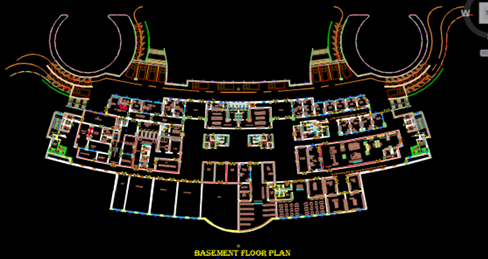
\includegraphics[width=0.6\linewidth]{i 1.png}
    \caption{ Basement Floor Plane}
    \label{fig:i 1}
\end{figure}

\\    1.Garage \ \ \ \ \ \ \ \ \ \ \ \ \ \ \ \ \ \ \ \ \ \ \ \ \ \ 2.Kitchen \ \ \ \ \ \ \ \ \ \ \ \ \ \ \ \ \ \ \ \ \ \ \ \ 3.Laundry \ \ \ \ \ \ \ \ \ \ \ \  
\\ 4.Store \ \ \ \ \ \ \ \ \ \ \ \ \ \ \ \ \ \ \ \ \ \ \ \ \ \ \ \ \ 5.Medical gas \ \ \ \ \ \ \ \ \ \ \ \  \ \ \ \ \  6.Electrical room \ \ \ \ \ \ \ \ \ \ \ \ 
\\7.Body holding room \ \ \ \ \ \  8.Pathology area \ \ \ \ \ \ \ \ \ \ \ \ \ 9.Autopthy room  
\\10.Control room \ \ \ \ \ \ \ \ \ \ \ \ \ 11.ToiletsHVAC ROOM
\begin{itemize}
    \item Basement area =4600 m
\end{itemize}


	    
	    \item \textbf{Ground}
	    \begin{figure}[h!]
    \centering
    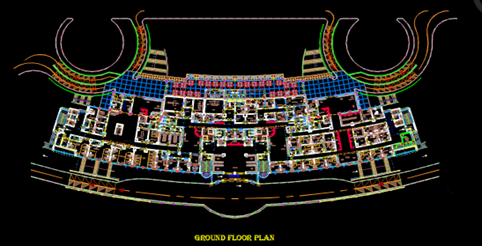
\includegraphics[width=0.6\linewidth]{i 2.png}
    \caption{ Ground Floor Plane}
    \label{fig:i 2}
\end{figure}
\\1.Laboratory \ \ \ \ \ \  \ \ \ \ \ \ \ \ \ \  \ \ \ 2.Teething lab \ \ \ \ \ \ \ \ \ \  \ \ \ \ \ \ \ \ 3.Ophthalmology
\\4.Pharmacy \ \ \ \ \ \  \ \ \ \ \ \ \ \ \ \  \ \ \ \ \  5.Dentistry clinic \ \ \ \ \ \ \ \ \ \ \ \ \ 6.Ultraviolet clinic
\\ 7.Dermatology clinic \ \ \ \ \ \ 8.Staff lounge \ \ \ \ \ \ \ \ \ \ \ \ \ \ \ \ \ \  9.Restaurant
\\ 10.C.U \ \ \ \ \ \ \ \  \ \ \ \ \ \ \ \ \ \  \ \ \ \ \ \ \ \ \ \ 11.Echo \ \ \ \ \ \ \ \ \ \ \ \ \ \ \  \ \ \ \ \ \ \ \ \ \ \ \ \ 12.M.R
\begin{itemize}
    \item Ground area=4600 m2
\end{itemize}


\newpage
	    
	    \item \textbf{First floor}
	        \begin{figure}[h!]
    \centering
    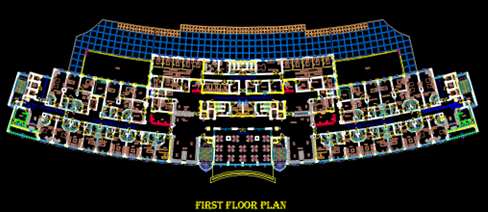
\includegraphics[width=0.8\linewidth]{i 3.png}
    \caption{ First Floor Plane}
    \label{fig:i 3}
\end{figure}
\\1.Cafeteria \ \ \ \ \ \ \ \ \ \ \ \ \ \ \ \ \ \ \ \ \  2.Patient room  \ \ \ \ \ \ \ \ \ \ \ \ \ \ \ \ \ \ 3.Linen
\\4.Isolation \ \ \ \ \ \ \ \ \ \ \ \ \ \ \ \ \ \ \ \ \  5.Training room  \ \ \ \ \ \ \ \ \ \ \ \ \ \ \ \  6.Exam treatment
\\7.Consultation \ \ \ \ \ \ \ \ \ \ \ \ \ \ \  8.Dialysis bay

\begin{itemize}
    \item First floor area=3010 $m^2$
\end{itemize}

	    
	    \item \textbf{Second floor}
	          \begin{figure}[h!]
    \centering
    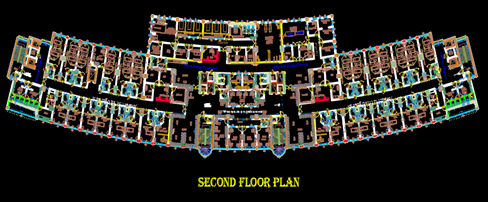
\includegraphics[width=0.8\linewidth]{i 4.png}
    \caption{ Second Floor Plane}
    \label{fig:i 4}
\end{figure}

\\1.Lasre Therapy \ \ \ \ \ \ \ \ \ \ \ \ \   2.Wax room \ \ \ \ \ \ \ \ \ \ \ \ \ \ \  \ \ \ \ \ 3.Magneto Therapy
\\4.Changing room  \ \ \ \ \ \ \ \ \ \ \  5.medical gas piping \ \ \ \ \ \ \   6.patient room
\\7.office \ \ \ \ \ \ \ \ \ \ \ \ \ \ \ \ \ \ \ \ \ \ \ \ \ \ \  8.anesthesia work room \ \ 9.operation room
\\10.recovery
\begin{itemize}
    \item second floor area=3010 $m^2$
\end{itemize}
\newpage


	    
	    \item \textbf{Third floor}
	    \begin{figure}[h!]
    \centering
    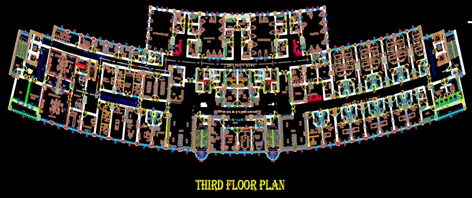
\includegraphics[width=0.8\linewidth]{i 5.png}
    \caption{ Third Floor Plane}
    \label{fig:i 5}
\end{figure}
\\1.Examination \ \ \ \ \ \ \ \ \ \ \ \ \ \ \ \ 2.Special care \ \ \ \ \ \ \ \ \ \ \ \ \ \ \ \ 3.Isolation
\\4.C.U \ \ \ \ \ \ \ \  \ \ \ \ \ \ \ \ \ \  \ \ \ \ \ \ \ \ \ \ \ 5.D.U \ \ \ \ \ \ \ \ \ \ \ \ \ \ \ \ \ \ \ \ \ \ \ \ \ \ \ \ \ 6.Manager office 
\\7.anesthesia work room \  8.operation room \ \ \ \ \ \ \ \ \ \ \  9.recovery
\begin{itemize}
    \item Third floor area =3010 $m^2$
\end{itemize}


	    \item \textbf{Fourth floor} 
	     \begin{figure}[h!]
    \centering
    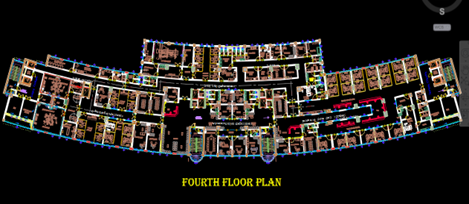
\includegraphics[width=0.8\linewidth]{i 6.png}
    \caption{ Fourth Floor Plane}
    \label{fig:i 6}
\end{figure}

\\1.Changing room \ \ \ \ \ \ \ \ \ \  2.medical gas piping \ \ \ \ \ \  3.patient room
\\4.office \ \ \ \ \ \ \ \ \ \ \ \ \ \ \ \ \ \ \ \ \ \ \ \ \ \ 5.anesthesia work room \  6.operation room
\\7.recovery \ \ \ \ \ \ \ \ \ \ \ \ \ \ \ \ \ \ \ \ \ 8.Dr lounge \ \ \ \ \ \ \ \ \ \ \ \ \ \ \  \ \ \ \ \  9.Staff lounge
\begin{itemize}
    \item Fourth floor area =3010 $m^2$
\end{itemize}
\newpage


	    
	    \item \textbf{Fifth floor}
	        \begin{figure}[h!]
    \centering
    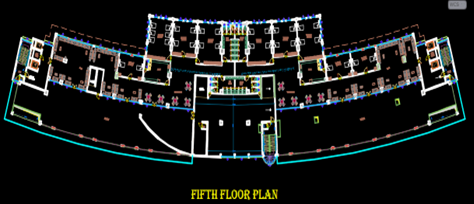
\includegraphics[width=0.8\linewidth]{i 7.png}
    \caption{ Fifth Floor Plane}
    \label{fig:i 7}
\end{figure}
\\1.Bedroom \ \ \ \ \ \ \ \ \ \ \ \ \ \ \ \ \ \ \ 2.Dining area \ \ \ \ \ \ \ \ \ \ \ \ \ \ \ \ \ 3.Terrace
\\4.Salon \ \ \  \ \ \ \ \ \ \ \ \ \  \  \ \ \ \ \ \ \ \ \ \ \ 5.Store
\begin{itemize}
    \item Fifth floor area=1800 $m^2$
\end{itemize}


	    
	\end{itemize}
\part {Load Estimation}

\chapter{Load Estimation}
%----------------------------------------------------------------------------------------
%	CHAPTER 1
%----------------------------------------------------------------------------------------

\chapterimage{load estimation.png} % Chapter heading image


\section{Load Estimation }
Electrical Load Estimation is very important in the early design stage because it helps to:
\begin{itemize}
\item  Plan the connection to upstream network and MV circuit configurations.
\item Plan the transformers substations and the main switchgear room.
\item Apply to Power Company for supply.
\item Calculate initial budget for the electrical works.
 \end{itemize}
\section{Important definitions}
\begin{enumerate}
\item \textbf {Connected load:}
\\It is the Sum of all the loads connected to the electrical system, usually expressed in watts.
\item \textbf {Demand load:}
\\It is the electric load at the receiving terminals averaged over a specified demand interval of time,usually15 min., 30 min., or 1 hour based upon the particular utility’s demand interval. Demand
may be expressed in amperes, kilo-amperes, kilo-watts, Kilo-vars, or Kilo-Volt- Amperes.
\item \textbf {Maximum demand:}
\\It is the greatest of all demands that have occurred during a specified period of time such as 5 minutes, 15 minutes, 30minutes or one hour. For utility billing purposes the period of time is generally one month.
\item \textbf {Demand factor:}
\\(in IEC, Factor of maximum utilization KU): In normal operating conditions the power consumption off-load is sometimes less than that indicated as its nominal power rating. The demand factor is the ratio of the maximum demand on system to the total connected load of the system. Demand factor= Maximum demand load/ Total load connected.
\end{enumerate}
%%%%%%%%%%%%%%%%%%%%%%%%%%%%%%%%%%%%%
\section{Load estimation depend on}
\begin{enumerate}
\item Lighting Power
\item Power (Sockets)
\item HVAC
\item Others (Lifts, Fire pump, Laundry, Medical equipment, Water pump)
\end{enumerate}
%%%%%%%%%%%%%%%%%%%%%%%%%%%%%%%%%%%%%
\section{Types of loads}
\begin{itemize}
\item \textbf {Residential loads}
\\Cities & the countries
\item \textbf {Commercial loads &services}
\\Hospitals, hotels, theatres, playground & airports
\item \textbf {Industrial loads}
\\Includes small and large factories.
\item \textbf {Lighting loads}
\\Includes Incandescent & Fluorescent lamps, Neon lights, &Mercury vapor, Sodium vapor,and Metal Halide lights.
\end{itemize}
%%%%%%%%%%%%%%%%%%%%%%%%%%%%%%%%%%%%%
\section{Load Estimation Calculations}
In first we should calculate the area of project and calculated the power needed according to Egyptian code or according to NEC Code as shown in figure \ref{fig:fikry 1}.
\begin{figure}[h]
    \centering
    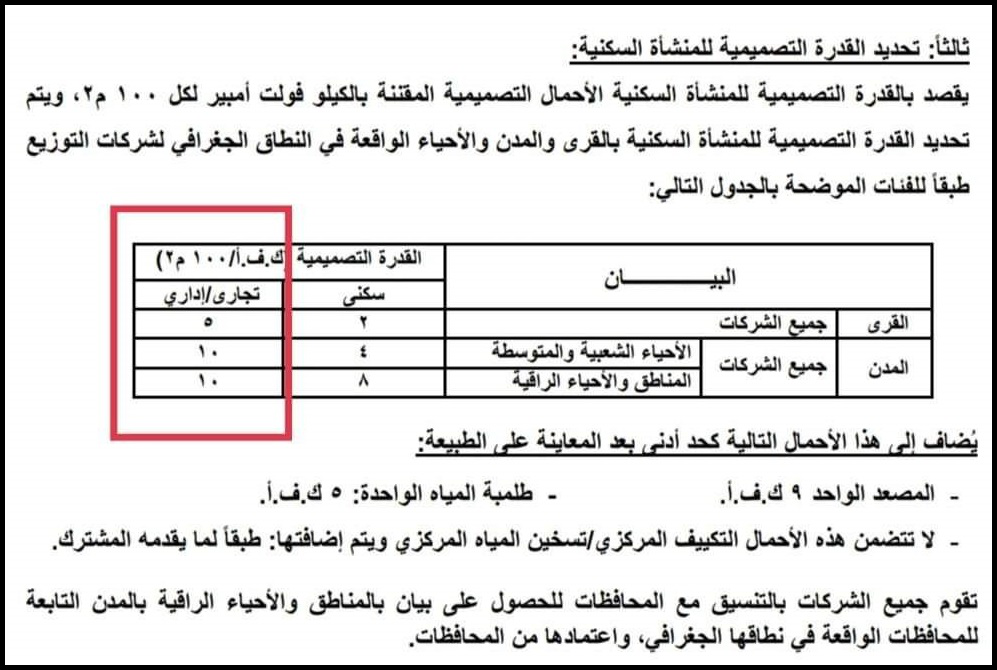
\includegraphics[width=0.80\linewidth]{fikry 1.png}
    \caption{Design Capacity (For The Residential Facility)}
    \label{fig:fikry 1}
\end{figure}
%%%%%
\begin{table}[!h]
\centering
\caption{Residential Buildings Less Than a Height of 15 Floors}
\arrayrulecolor{black}
\begin{tabular}{!{\color[rgb]{0.557,0.667,0.859}\vrule}c!{\color{black}\vrule}c!{\color[rgb]{0.557,0.667,0.859}\vrule}c!{\color[rgb]{0.557,0.667,0.859}\vrule}} 
\hline
\multicolumn{3}{!{\color[rgb]{0.267,0.447,0.769}\vrule}c!{\color{black}\vrule}}{{\cellcolor[rgb]{0.267,0.447,0.769}}\textbf{\textcolor{white}{Load demand per 100 square meters KVA}}}  \\ 
\hline
\rowcolor[rgb]{0.851,0.886,0.953} \multicolumn{2}{!{\color[rgb]{0.557,0.667,0.859}\vrule}c!{\color{black}\vrule}}{\textbf{Residential}} & \textbf{Administrative}                       \\ 
\hline
low cost
  housing                                    & 1.5-2                                                                           & \multirow{3}{*}{~
  6-12}                     \\ 
\hhline{>{\arrayrulecolor[rgb]{0.557,0.667,0.859}}|>{\arrayrulecolor{black}}--~>{\arrayrulecolor[rgb]{0.557,0.667,0.859}}|}
{\cellcolor[rgb]{0.851,0.886,0.953}}average
  housing & {\cellcolor[rgb]{0.851,0.886,0.953}}2.5-4                                       &                                               \\ 
\arrayrulecolor{black}\cline{1-2}
luxury
  housing                                      & 6-10                                                                            &                                               \\
\hline
\end{tabular}
\arrayrulecolor{black}
\end{table}
%%%%%%
\begin{table}[!h]
\centering
\caption{Residential Buildings More Than a Height of 15 Floors}
\arrayrulecolor{black}
\begin{tabular}{!{\color[rgb]{0.557,0.667,0.859}\vrule}c!{\color{black}\vrule}c!{\color[rgb]{0.557,0.667,0.859}\vrule}} 
\hline
\multicolumn{2}{!{\color[rgb]{0.267,0.447,0.769}\vrule}c!{\color{black}\vrule}}{{\cellcolor[rgb]{0.267,0.447,0.769}}\textbf{\textcolor{white}{Load demand per 100 square meters KVA}}}  \\ 
\hline
\rowcolor[rgb]{0.851,0.886,0.953} Residential & Administrative                                                                                                                          \\ 
\hline
8-10                                          & 12                                                                                                                                      \\
\hline
\end{tabular}
\arrayrulecolor{black}
\end{table}

%%%%%%%
\begin{table}[!h]
\centering
\caption{Extra Load Calculation}
\arrayrulecolor{black}
\begin{tabular}{!{\color{black}\vrule}c!{\color{black}\vrule}c!{\color{black}\vrule}c!{\color{black}\vrule}c!{\color{black}\vrule}c!{\color{black}\vrule}c!{\color{black}\vrule}c!{\color{black}\vrule}c!{\color{black}\vrule}c!{\color{black}\vrule}}
\multicolumn{4}{c}{{\cellcolor[rgb]{1,0.949,0.8}}\textbf{ HVAC loads (Basement) }}                                                                                    & \multicolumn{1}{c}{} & \multicolumn{4}{c}{{\cellcolor[rgb]{1,0.949,0.8}}\textbf{ HVAC loads (ROOF) }}                                                                                           \\ 
\hhline{|----~----|}
{\cellcolor{yellow}}Unit                           & {\cellcolor{yellow}}load (KW)        & {\cellcolor{yellow}}no.unints     & {\cellcolor{yellow}}Total(KW)         &                      & {\cellcolor{yellow}}Unit                          & {\cellcolor{yellow}}load (KW)          & {\cellcolor{yellow}}no.unints     & {\cellcolor{yellow}}Total(KW)           \\ 
\hhline{|----~----|}
{\cellcolor[rgb]{0.663,0.816,0.557}}FCU-01         & 2.04                                 & 1                                 & 2.04                                  &                      & {\cellcolor[rgb]{0.663,0.816,0.557}}FCU-05        & 3.7                                    & 1                                 & 3.7                                     \\ 
\hhline{|----~----|}
{\cellcolor[rgb]{0.663,0.816,0.557}}FCU-02         & 2.7                                  & 7                                 & 18.9                                  &                      & {\cellcolor[rgb]{0.663,0.816,0.557}}FCU-06        & 4.25                                   & 6                                 & 25.5                                    \\ 
\hhline{|----~----|}
{\cellcolor[rgb]{0.663,0.816,0.557}}FCU-03         & 2.6                                  & 8                                 & 20.8                                  &                      & {\cellcolor[rgb]{0.663,0.816,0.557}}FCU-07        & 4.25                                   & 2                                 & 8.5                                     \\ 
\hhline{|----~----|}
{\cellcolor[rgb]{0.663,0.816,0.557}}FCU-04         & 3.6                                  & 3                                 & 10.8                                  &                      & {\cellcolor[rgb]{0.663,0.816,0.557}}FCU-08        & 6.37                                   & 2                                 & 12.74                                   \\ 
\hhline{|----~----|}
{\cellcolor[rgb]{0.663,0.816,0.557}}FCU-05         & 3.7                                  & 1                                 & 3.7                                   &                      & {\cellcolor[rgb]{0.663,0.816,0.557}}FCU-10        & 8.56                                   & 16                                & 136.96                                  \\ 
\hhline{|----~----|}
{\cellcolor[rgb]{0.663,0.816,0.557}}FCU-06         & 4.25                                 & 1                                 & 4.25                                  &                      & {\cellcolor[rgb]{0.663,0.816,0.557}}EXF1          & 0.75                                   & 1                                 & 0.75                                    \\ 
\hhline{|----~----|}
{\cellcolor[rgb]{0.663,0.816,0.557}}FCU-09         & 6.37                                 & 5                                 & 31.85                                 &                      & {\cellcolor[rgb]{0.663,0.816,0.557}}EXF2          & 2.2                                    & 1                                 & 2.2                                     \\ 
\hhline{|----~----|}
{\cellcolor[rgb]{0.663,0.816,0.557}}FCU-10         & 8.56                                 & 2                                 & 17.12                                 &                      & {\cellcolor[rgb]{0.663,0.816,0.557}}EXF3          & 3.7                                    & 1                                 & 3.7                                     \\ 
\hhline{|----~----|}
{\cellcolor[rgb]{0.663,0.816,0.557}}AHU-01         & 2.2                                  & 1                                 & 2.2                                   &                      & {\cellcolor[rgb]{0.663,0.816,0.557}}EXF4          & 0.37                                   & 1                                 & 0.37                                    \\ 
\hhline{|----~----|}
{\cellcolor[rgb]{0.663,0.816,0.557}}AHU-02         & 3.7                                  & 1                                 & 3.7                                   &                      & {\cellcolor[rgb]{0.663,0.816,0.557}}EXF5          & 5.6                                    & 1                                 & 5.6                                     \\ 
\hhline{|----~----|}
{\cellcolor[rgb]{0.663,0.816,0.557}}AHU-03         & 30                                   & 1                                 & 30                                    &                      & {\cellcolor[rgb]{0.663,0.816,0.557}}EXF6          & 2.2                                    & 1                                 & 2.2                                     \\ 
\hhline{|----~----|}
{\cellcolor[rgb]{0.663,0.816,0.557}}AHU-04         & 7.5                                  & 1                                 & 7.5                                   &                      & {\cellcolor[rgb]{0.663,0.816,0.557}}EXF7          & 1.1                                    & 1                                 & 1.1                                     \\ 
\hhline{|----~----|}
{\cellcolor[rgb]{0.663,0.816,0.557}}AHU-05         & 5.6                                  & 1                                 & 5.6                                   &                      & {\cellcolor[rgb]{0.663,0.816,0.557}}EXF8          & 1.5                                    & 1                                 & 1.5                                     \\ 
\hhline{|----~----|}
{\cellcolor[rgb]{0.663,0.816,0.557}}AHU-06         & 5.6                                  & 1                                 & 5.6                                   &                      & {\cellcolor[rgb]{0.663,0.816,0.557}}EXF9          & 1.5                                    & 1                                 & 1.5                                     \\ 
\hhline{|----~----|}
{\cellcolor[rgb]{0.663,0.816,0.557}}\textbf{ SUM } & {\cellcolor{yellow}}\textbf{ 88.4 }  & {\cellcolor{yellow}}\textbf{ 34 } & {\cellcolor{yellow}}\textbf{ 164.06 } &                      & {\cellcolor[rgb]{0.663,0.816,0.557}}EXF10         & 1.5                                    & 1                                 & 1.5                                     \\ 
\hhline{----~----|}
\multicolumn{1}{c}{}                               & \multicolumn{1}{c}{}                 & \multicolumn{1}{c}{}              & \multicolumn{1}{c}{}                  &                      & {\cellcolor[rgb]{0.663,0.816,0.557}}EXF11         & 1.1                                    & 1                                 & 1.1                                     \\ 
\hhline{>{\arrayrulecolor[rgb]{1,0.949,0.8}}----~>{\arrayrulecolor{black}}----|}
\multicolumn{4}{c}{{\cellcolor[rgb]{1,0.949,0.8}}\textbf{ HVAC loads (GROUND) }}                                                                                      &                      & {\cellcolor[rgb]{0.663,0.816,0.557}}EXF12         & 1.5                                    & 1                                 & 1.5                                     \\ 
\hhline{|----~----|}
{\cellcolor{yellow}}Unit                           & {\cellcolor{yellow}}load (KW)        & {\cellcolor{yellow}}no.unints     & {\cellcolor{yellow}}Total(KW)         &                      & {\cellcolor[rgb]{0.663,0.816,0.557}}EXF13         & 1.1                                    & 1                                 & 1.1                                     \\ 
\hhline{|----~----|}
{\cellcolor[rgb]{0.663,0.816,0.557}}FCU-01         & 2.04                                 & 4                                 & 8.16                                  &                      & {\cellcolor[rgb]{0.663,0.816,0.557}}EXF14         & 1.5                                    & 1                                 & 1.5                                     \\ 
\hhline{|----~----|}
{\cellcolor[rgb]{0.663,0.816,0.557}}FCU-02         & 2.56                                 & 13                                & 33.28                                 &                      & {\cellcolor[rgb]{0.663,0.816,0.557}}EXF15         & 1.5                                    & 1                                 & 1.5                                     \\ 
\hhline{|----~----|}
{\cellcolor[rgb]{0.663,0.816,0.557}}FCU-03         & 2.59                                 & 15                                & 38.85                                 &                      & {\cellcolor[rgb]{0.663,0.816,0.557}}EXF16         & 2.2                                    & 1                                 & 2.2                                     \\ 
\hhline{|----~----|}
{\cellcolor[rgb]{0.663,0.816,0.557}}FCU-04         & 3.62                                 & 6                                 & 21.72                                 &                      & {\cellcolor[rgb]{0.663,0.816,0.557}}EXF17         & 3.7                                    & 1                                 & 3.7                                     \\ 
\hhline{|----~----|}
{\cellcolor[rgb]{0.663,0.816,0.557}}FCU-05         & 3.69                                 & 6                                 & 22.14                                 &                      & {\cellcolor[rgb]{0.663,0.816,0.557}}EXF18         & 3.7                                    & 1                                 & 3.7                                     \\ 
\hhline{|----~----|}
{\cellcolor[rgb]{0.663,0.816,0.557}}FCU-06         & 3.75                                 & 1                                 & 3.75                                  &                      & {\cellcolor[rgb]{0.663,0.816,0.557}}EXF19         & 3.7                                    & 1                                 & 3.7                                     \\ 
\hhline{|----~----|}
{\cellcolor[rgb]{0.663,0.816,0.557}}\textbf{ SUM}  & {\cellcolor{yellow}}\textbf{ 18.25 } & {\cellcolor{yellow}}\textbf{ 45 } & {\cellcolor{yellow}}\textbf{ 127.9 }  &                      & {\cellcolor[rgb]{0.663,0.816,0.557}}EXF20         & 7.5                                    & 1                                 & 7.5                                     \\ 
\hhline{----~----|}
\multicolumn{1}{c}{}                               & \multicolumn{1}{c}{}                 & \multicolumn{1}{c}{}              & \multicolumn{1}{c}{}                  &                      & {\cellcolor[rgb]{0.663,0.816,0.557}}EXF21         & 3.7                                    & 1                                 & 3.7                                     \\ 
\hhline{>{\arrayrulecolor[rgb]{1,0.949,0.8}}----~>{\arrayrulecolor{black}}----|}
\multicolumn{4}{c}{{\cellcolor[rgb]{1,0.949,0.8}}\textbf{ HVAC loads (1st) }}                                                                                         &                      & {\cellcolor[rgb]{0.663,0.816,0.557}}EXF22         & 3.7                                    & 1                                 & 3.7                                     \\ 
\hhline{|----~----|}
{\cellcolor{yellow}}Unit                           & {\cellcolor{yellow}}load (KW)        & {\cellcolor{yellow}}no.unints     & {\cellcolor{yellow}}Total(KW)         &                      & {\cellcolor[rgb]{0.663,0.816,0.557}}EXF23         & 1.5                                    & 1                                 & 1.5                                     \\ 
\hhline{|----~----|}
{\cellcolor[rgb]{0.663,0.816,0.557}}FCU-03         & 2.6                                  & 2                                 & 5.2                                   &                      & {\cellcolor[rgb]{0.663,0.816,0.557}}FAHU1         & 7.5                                    & 1                                 & 7.5                                     \\ 
\hhline{|----~----|}
{\cellcolor[rgb]{0.663,0.816,0.557}}FCU-04         & 3.6                                  & 10                                & 36                                    &                      & {\cellcolor[rgb]{0.663,0.816,0.557}}FAHU2         & 7.5                                    & 1                                 & 7.5                                     \\ 
\hhline{|----~----|}
{\cellcolor[rgb]{0.663,0.816,0.557}}FCU-05         & 3.7                                  & 15                                & 55.5                                  &                      & {\cellcolor[rgb]{0.663,0.816,0.557}}AHU7          & 7.5                                    & 1                                 & 7.5                                     \\ 
\hhline{|----~----|}
{\cellcolor[rgb]{0.663,0.816,0.557}}FCU-06         & 4.3                                  & 6                                 & 25.8                                  &                      & {\cellcolor[rgb]{0.663,0.816,0.557}}AHU8          & 5.6                                    & 1                                 & 5.6                                     \\ 
\hhline{|----~----|}
{\cellcolor[rgb]{0.663,0.816,0.557}}FCU-07         & 4.3                                  & 3                                 & 12.9                                  &                      & {\cellcolor[rgb]{0.663,0.816,0.557}}AHU9          & 7.5                                    & 1                                 & 7.5                                     \\ 
\hhline{|----~----|}
{\cellcolor[rgb]{0.663,0.816,0.557}}FCU-10         & 8.7                                  & 3                                 & 26.1                                  &                      & {\cellcolor[rgb]{0.663,0.816,0.557}}AHU10         & 7.5                                    & 1                                 & 7.5                                     \\ 
\hhline{|----~----|}
{\cellcolor[rgb]{0.663,0.816,0.557}}\textbf{ SUM}  & {\cellcolor{yellow}}\textbf{ 27.2 }  & {\cellcolor{yellow}}\textbf{ 39 } & {\cellcolor{yellow}}\textbf{ 161.5 }  &                      & {\cellcolor[rgb]{0.663,0.816,0.557}}AHU11         & 5.6                                    & 1                                 & 5.6                                     \\ 
\hhline{----~----|}
\multicolumn{1}{c}{}                               & \multicolumn{1}{c}{}                 & \multicolumn{1}{c}{}              & \multicolumn{1}{c}{}                  &                      & {\cellcolor[rgb]{0.663,0.816,0.557}}AHU12         & 7.5                                    & 1                                 & 7.5                                     \\ 
\hhline{>{\arrayrulecolor[rgb]{1,0.949,0.8}}----~>{\arrayrulecolor{black}}----|}
\multicolumn{4}{c}{{\cellcolor[rgb]{1,0.949,0.8}}HVAC loads (2nd)}                                                                                                    &                      & {\cellcolor[rgb]{0.663,0.816,0.557}}AHU13         & 18.6                                   & 1                                 & 18.6                                    \\ 
\hhline{|----~----|}
{\cellcolor{yellow}}Unit                           & {\cellcolor{yellow}}load (KW)        & {\cellcolor{yellow}}no.unints     & {\cellcolor{yellow}}Total(KW)         &                      & {\cellcolor[rgb]{0.663,0.816,0.557}}AHU14         & 7.5                                    & 1                                 & 7.5                                     \\ 
\hhline{|----~----|}
{\cellcolor[rgb]{0.663,0.816,0.557}}FCU-02         & 3.57                                 & 1                                 & 3.57                                  &                      & {\cellcolor[rgb]{0.663,0.816,0.557}}P-01          & 75                                     & 1                                 & 75                                      \\ 
\hhline{|----~----|}
{\cellcolor[rgb]{0.663,0.816,0.557}}FCU-03         & 2.6                                  & 7                                 & 18.2                                  &                      & {\cellcolor[rgb]{0.663,0.816,0.557}}P-02          & 75                                     & 1                                 & 75                                      \\ 
\hhline{|----~----|}
{\cellcolor[rgb]{0.663,0.816,0.557}}FCU-04         & 3.6                                  & 4                                 & 14.4                                  &                      & {\cellcolor[rgb]{0.663,0.816,0.557}}~             & ~                                      & ~                                 & ~                                       \\ 
\hhline{|----~----|}
{\cellcolor[rgb]{0.663,0.816,0.557}}FCU-05         & 3.7                                  & 25                                & 92.5                                  &                      & {\cellcolor[rgb]{0.663,0.816,0.557}}P-04          & 37                                     & 1                                 & 37                                      \\ 
\hhline{|----~----|}
{\cellcolor[rgb]{0.663,0.816,0.557}}FCU-06         & 4.3                                  & 1                                 & 4.3                                   &                      & {\cellcolor[rgb]{0.663,0.816,0.557}}~             & ~                                      & ~                                 & ~                                       \\ 
\hhline{|----~----|}
{\cellcolor[rgb]{0.663,0.816,0.557}}FCU-07         & 4.3                                  & 1                                 & 4.3                                   &                      & {\cellcolor[rgb]{0.663,0.816,0.557}}P-06          & 37                                     & 1                                 & 37                                      \\ 
\hhline{|----~----|}
{\cellcolor[rgb]{0.663,0.816,0.557}}FCU-10         & 8.7                                  & 1                                 & 8.7                                   &                      & {\cellcolor[rgb]{0.663,0.816,0.557}}CHILLER       & 700                                    & 2                                 & 1400                                    \\ 
\hhline{|----~----|}
{\cellcolor[rgb]{0.663,0.816,0.557}}\textbf{ SUM}  & {\cellcolor{yellow}}\textbf{ 30.77 } & {\cellcolor{yellow}}\textbf{ 40 } & {\cellcolor{yellow}}\textbf{ 145.97 } &                      & {\cellcolor[rgb]{0.663,0.816,0.557}}\textbf{ SUM} & {\cellcolor{yellow}}\textbf{ 1090.25 } & {\cellcolor{yellow}}\textbf{ 66 } & {\cellcolor{yellow}}\textbf{ 1950.52 }  \\
\hhline{|----~----|}
\end{tabular}
\arrayrulecolor{black}
\end{table}%%%%%%%
\begin{figure}[!h]
    \centering
    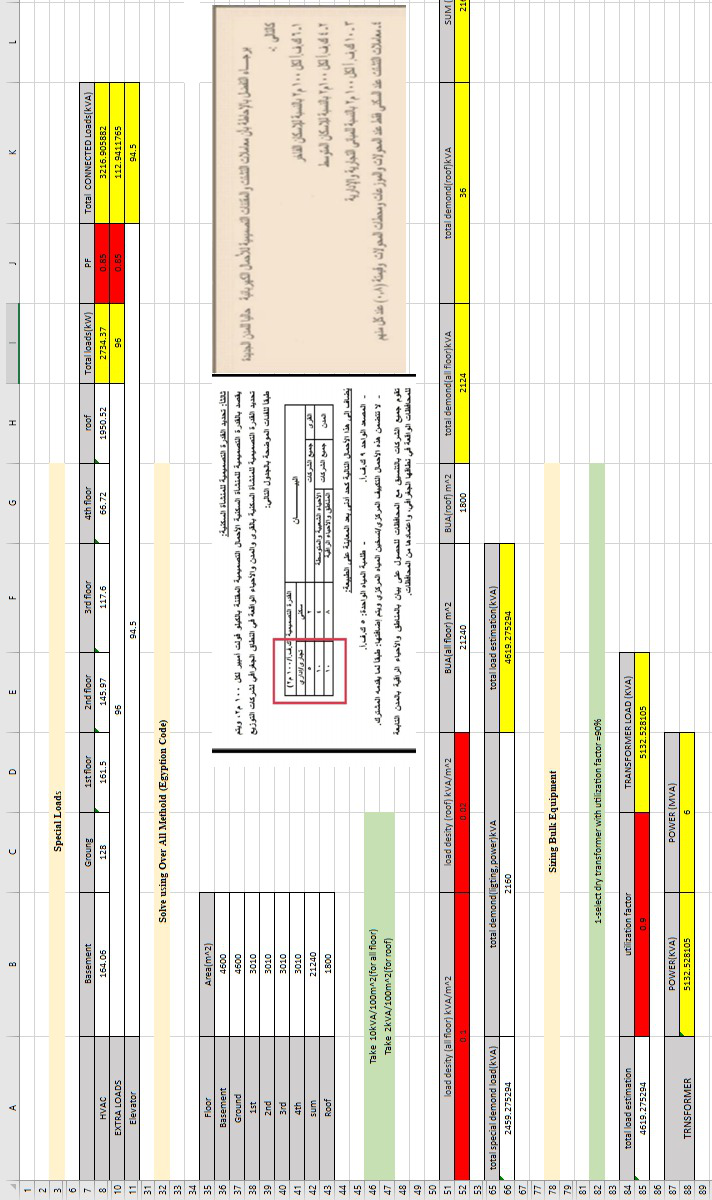
\includegraphics[width=0.90\linewidth]{fikry 4.png}
    \caption{Excel Sheet}
    \label{fig:fikry 4}
\end{figure}
%%%%%%%
\begin{itemize}
\item \textbf {Transformer Sizing}
\\ { 5MVA } ABB / DRY Type
\end{itemize}

%%%%%%%%%%%%%%%%%%%%%%%%%%%%%%%%%%%%%%%%%%%%%%%%%%%%%%


%-----------------------------------------------------------------------------
%	CHAPTER 2
%--------------------------------------------------------------------------------
\part{Lighting}
\chapterimage{lighting.png} % Chapter heading image
\chapter{Lighting}
\section{Lighting in distribution systems}
Light is the prime factor in the human life as all activities of human depend upon the light. Where there is no natural light, a source of artificial light was needed. Light may be produced by passing electric currents through filaments as in the incandescent lamps, through arcs between carbon or metal rods, or through suitable gases as in neon and other gas tubes. In some forms of lamps the light is due to fluorescence excited by radiation arising from the passage of electricity through mercury vapor. We will plan the distribution system in a big building (Health care Hospital center). And the various types of loads in the building like lighting.\\
\textbf {Light:} It is defined as the radiant energy from a hot body, which produces the visual sensation upon the human eye this chapter discusses the procedures to efficient or precisely effective distribution of lighting using first manual calculations – but it is not appropriate as we seek more efficiency. so, we decided to program our excel program, .Then we use different programs of lighting calculations and distribution. Finally, we Compare between results of them all and choose the best lighting solution.

%------------------------------------------------

\section{Requirements of a good lighting scheme}
Requirements of a good lighting scheme:
\begin{itemize}
\item  Provide adequate illumination.
\item Provide uniform illumination all over the working plan.
\item Provide light of suitable color.
\item Avoid glare and hard shadows.
\item Minimum Cost.
 \end{itemize}
 %%%%%%%%%%%%%%%%%%%%%
 \section{Definitions Used In Lighting}
\begin{enumerate}
\item \textbf {Candela:}
\\International unit (SI) of luminous intensity. This term evolved from considering a standard candle as the basis of evaluating the relative intensity of a source.
\item \textbf {Candle Power Distribution Curve:}
\\A graphic presentation of the distribution of light intensity of a lamp or luminaire.
\item \textbf {Illumination (E):}
\\The quantity of light (measured in Lux) at a point on a surface.
\item \textbf {Lux (lumen/m2):}
\\SI (international system) unit of illumination. One lumen uniformly distributed over an area of one square meter.
\item \textbf {Lumen:}
\\The international unit of luminous flux or quantity of light. It is defined as the energy in the form of light waves radiated per second from a luminous body.
\item \textbf {Lux (Luminaire:}
\\A complete lighting unit consisting of a lamp (or lamps) together with the parts designed to distribute the light, position and protect the lamps, and connect them to the power supply. This is sometimes referred to as a "fixture".
\item \textbf {Lux (Lamp efficiency:}
\\It is the amount of output lumen per watt.
\item \textbf {Mounting Height:}
\\Distance from the bottom of the fixture to either the floor or work plane, depending on usage as shown in figure \ref{fig:fikry 5}.
\begin{figure}[!h]
    \centering
    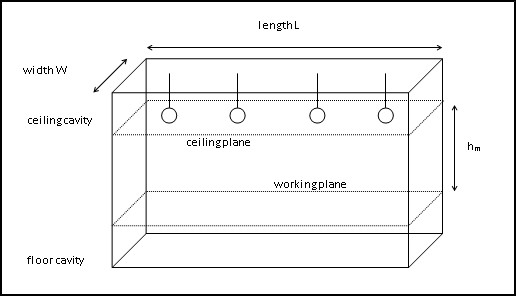
\includegraphics[width=0.5\linewidth]{fikry 5.png}
    \caption{Mounting Height According to Work Plane}
    \label{fig:fikry 5}
\end{figure}
\item \textbf {Maintenance Factor:}
\\It is the ratio between illuminations under normal working conditions to illumination when everything is clean.
\item \textbf {Utilization factor:}
\\It is the ratio of the lumen actually received by a particular surface to the total lumen emitted by
luminous source.
\end{enumerate}
 \section{The value of this coefficient depends on }
\begin{enumerate}
\item \textbf {The area to be illuminated}
\item \textbf {The height at which the lamps are fitted.}
\item \textbf {The colors of surrounding walls and ceiling.}
\item \textbf {The type of lighting (direct or indirect).}
\item \textbf {Efficiency of Lamp } 
\\It is defined as the ratio between the lumen output to the wattage of the lamp.
\begin{align} 
\begin{split}
\eta =\frac{Total\ \ Lumens}{Total\ \ Wattage \ \ lumen\ \ per\ \ watt}
\end{split}					
\end{align} 
\item \textbf {Light Loss Factor:}
\\The product of all considered factors that contribute to a lighting system's depreciated light output over a period of time, including dirt and lamp lumen depreciation. 
\item \textbf {Luminous intensity (I):}
\\Is the amount of light that a light source emits per unit solid angle (lumen /steroidal). 
\end{enumerate}
%%%%%%%%%%%%%%%%%%%%%%%
 \section{Factors affecting illumination and wattage}
 \begin{enumerate}
 \item \textbf {Utilization factor (U.F):}
\\(0.2 : 0.6) It is the ratio of the lumen actually received to the total Lumens emitted by the source, 

\\ \textbf {depends on:}  
\begin {itemize}
\item  {Room dimensions.}
\item  {Color of the walls.}
\item  {Type of lighting scheme.}
\item  {The height at which the lamps are fitted.}
\end {itemize}

\item \textbf {Maintenance factor (M.F):}
\\It is the ratio between illuminations under normal working conditions to the illumination when everything is clean. It depends on the rate of cleaning. M.F:
\begin {itemize}
\item  {0.8 for houses.}
\item  {0.3 for streets.}
\item  {0.6 :0.7 for schools and shopping centers.}
\end {itemize}

\item \textbf {Reflection factor:}
\\Due to the fact that light reflected by an angle of incidence when impinged on a surface.
 \end{enumerate}
%%%%%%%%%%%%%%%%%%%%%%%%
 \section{Types of lighting}
 \begin{enumerate}
 \item \textbf {Direct Lighting:}
 \\ In this type of lighting the light from the source falls directly on the object or the surface to be illuminated. More than 90\% of the total light flux is made to fall directly on the working plane. It is mainly used for industrial and outdoor lighting
\textbf {Properties of direct lighting:}
\begin {itemize}
\item  {Highly directional}
\item  {Strong glare reduction at certain angles}
\item  {Dark ceiling ( cave effect )}
\item  {Limited choice of work station layout}
\item  {Efficient energy}
\end {itemize}
 \item \textbf {Semi Direct Lighting: }
\\ [ 60.90\% ] of the total light flux is made to full down words directly .
 \item \textbf {General Diffusing Lighting:}
 \\ The total light flux thrown upward =total light flux falls downwards.
 \item \textbf {Semi Indirect Lighting:}
 \\ 60.90\% of total light flux is thrown upward to the ceiling and the rest reaches the working plane directly .It is mainly used for indoor light decoration purpose.
 \item \textbf {Indirect lighting:}
 \\ More than 90\% of the total light flux is thrown upwards to the ceiling and only 10\% reaches the working plane, it is used for decoration purpose in cinemas , theaters and hotels and workshops.   \\
\textbf {Properties of indirect lighting:}
\begin {itemize}
\item  {Diffuse lighting conditions}
\item  {Room gains in height}
\item  {Glare- free}
\item  {Workstations can be positioned anywhere}
\item  {Low energy efficiency}
\end {itemize}
 \end{enumerate}
 %%%%%%%%%%%%%%%%%
  \section{Factors influencing design }
  \\ many variables must be considered in order to achieve a properly lighting system design. In most cases voltage levels and fixture types will be dictated by client requirements 
 \\ \textbf {as the following:}
\begin {itemize}
\item {Tasks to be performed in the space}
\item {Layout of furniture and obstructions such as partitions}
\item {Type of lighting}
\item {Type of lamp}
\item {Shape of reflector}
\item {Room dimensions}
\item {Glare}
\item {Luminaire fixture}
\item {Lighting switching and control}
\item {Initial cost and operating cost}
\item {Hours of operation}
\item {Cleanliness of the area during operation availability of daylight}
\item {IP index}
\item {Type of ceiling}

\end {itemize}
%%%%%%%%%%%%%%%%%%%%%%%%
  \section{Types of Lamps}
\begin{enumerate}
    \item Filament Lamps 
    \begin{itemize}
        \item Incandescent type
        The incandescent lamp is the oldest electric light source still in general use. It is also the most varied as regards types as Shown in Figure \ref{fig:fikry 6}.\\
        Current is passed through a filament, which heats until it glows; it gives light close to natural light.
        \begin{figure}[!h]
    \centering
    
\includegraphics[width=0.5\linewidth]{fikry 6.png}
    \caption{Incandescent Lamp}
    \label{fig:fikry 6}
\end{figure}
\\ \textbf{Characteristics of incandescent lamp}
\begin{itemize}
 \item Less efficacious light source.
 \item Shorter lifetime than other light sources in most cases.
 \item Filament is sensitive to vibrations.
 \item Bulb can get very hot during operation.
Must be properly shielded because incandescent lamps can produce direct glare as a point source.
 \item Voltage fluctuation has more effect on the light output. That is why it requires proper line voltage.
\end{itemize}
The Advantages and Disadvantages of incandescent lamp Explained in the Table \ref{tab:Advantages and Disadvantages of incandescent lamp}
\begin{table}[!h]
\centering
\caption{Advantages and Disadvantages of Incandescent Lamp}
\label{tab:Advantages and Disadvantages of incandescent lamp}%
\arrayrulecolor{black}
\begin{tabular}{!{\color[rgb]{0.584,0.702,0.843}\vrule}l!{\color{black}\vrule}l!{\color[rgb]{0.584,0.702,0.843}\vrule}} 
\hline
\rowcolor[rgb]{0.31,0.506,0.741} \multicolumn{1}{!{\color[rgb]{0.31,0.506,0.741}\vrule}c}{\textbf{\textcolor{white}{Advantages}}}                                                           & \multicolumn{1}{c!{\color[rgb]{0.31,0.506,0.741}\vrule}}{\textcolor{white}{Disadvantages\textbf{}}}  \\ 
\hline
\rowcolor[rgb]{0.859,0.898,0.945} Lowest initial lamp cost                                                                                                                                  & Sensitive to shock  vibrations                                                                       \\ 
\hline
\begin{tabular}[c]{@{}l@{}}immediate starting, no time is required to\\heat electrodes or start the discharge process\end{tabular}                                                          & Low lamp efficacy 10:15 Lm/watt                                                                      \\ 
\hline
\rowcolor[rgb]{0.859,0.898,0.945} \begin{tabular}[c]{@{}>{\cellcolor[rgb]{0.859,0.898,0.945}}l@{}}Warm color is close to natural light, so gives\\good color rendering (100\%)\end{tabular} & Short lifetime (111-2000hrs)                                                                         \\ 
\hline
Good light control                                                                                                                                                                          & \begin{tabular}[c]{@{}l@{}}Lamp lifetime is affected by\\voltage fluctuations\end{tabular}           \\ 
\hline
\rowcolor[rgb]{0.859,0.898,0.945} Small size                                                                                                                                                & Low light output (Lumens per watt)                                                                   \\ 
\hline
~                                                                                                                                                                                           & High power losses                                                                                    \\ 
\hline
\rowcolor[rgb]{0.859,0.898,0.945} ~                                                                                                                                                         & High operating cost                                                                                  \\
\hline
\end{tabular}
\arrayrulecolor{black}
\end{table}
       \item Halogen lamp
     \\  It is a special type of incandescent lamp. The light output is more consistent than a standard incandescent lamp, the life hours is longer and smaller in size, because it is important for the halogen cycle to have a high bulb wall temperature which requires quartz or hard glass to be used.\\
       Better beam is possible because of the small size as shown in figure \ref{fig:fikry 7} .\\
       The current flows through a filament and heats it up, just as in incandescent lamp. These lamps
       generate a relatively large amount of heat. The halogen cycle increases the efficiency and extends the life hours compared with traditional incandescent lamp.\\
       Halogen lamp as Shown in Figure \ref{fig:fikry 7}
       
\\ \textbf{Characteristics of Halogen lamp}
\begin{itemize}
\item Longer life hours.
\item Higher luminous efficacy.
\item Easy to dimming.
\item Brilliant light.
\item Excellent color rendering.
\item Color: yellow
\item Color rendering factor: 100\%
\end{itemize}
\begin{figure}[!h]
    \centering
    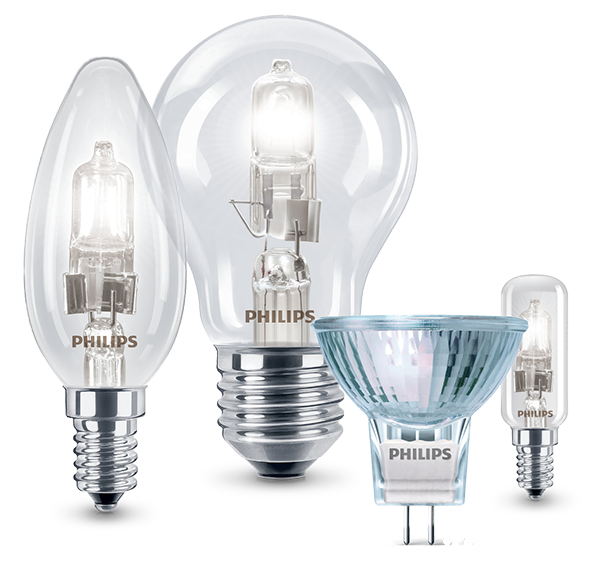
\includegraphics[width=0.5\linewidth]{fikry 7.png}
    \caption{Halogen Family Lamps (Philips)}
    \label{fig:fikry 7}
\end{figure}
       \item Reflector Lamp as shown in figure \ref{fig:fikry 8}
       \begin{itemize}
       \item has Low Power
       \item Reflector Lamp need to light reflector to enhance light distribution
       \item Reflector Lamp used for decoration, disco…
\end{itemize}
\\ Reflector Lamp Shown in Figure \ref{fig:fikry 8}
\begin{figure}[!h]
    \centering
    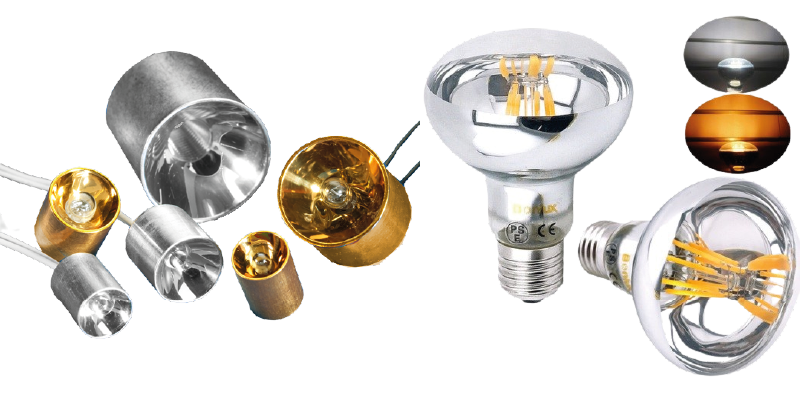
\includegraphics[width=0.5\linewidth]{fikry 8.png}
    \caption{Reflector Lamp}
    \label{fig:fikry 8}
\end{figure}
    \end{itemize}
    \item Gas Discharge Lamps
    \begin{itemize}
        \item Fluorescent
        The operation of these lamps depends on the gaseous discharge method, by creating an arc between two electrodes in a glass tube filled with an inner gas.\\
        Light is produced by phosphor coating on the inside of the glass, where it uses a ballast to produce high voltage to discharge the gas.
The Advantages and Disadvantages of Fluorescent lamp Explained in the Table \ref{tab:Advantages and Disadvantages of incandescent lamp}
\begin{table}[!h]
\centering
\caption{Advantages and Disadvantages of Fluorescent Lamp}
\label{tab:Advantages and Disadvantages of incandescent lamp}%
\arrayrulecolor{black}
\begin{tabular}{!{\color[rgb]{0.584,0.702,0.843}\vrule}l!{\color{black}\vrule}l!{\color[rgb]{0.584,0.702,0.843}\vrule}} 
\hline
\rowcolor[rgb]{0.31,0.506,0.741} \multicolumn{1}{!{\color[rgb]{0.31,0.506,0.741}\vrule}l}{\textbf{\textcolor{white}{Advantages}}}                                    & \multicolumn{1}{l!{\color[rgb]{0.31,0.506,0.741}\vrule}}{\textbf{\textcolor{white}{Disadvantages}}}                                                          \\ 
\hline
\rowcolor[rgb]{0.859,0.898,0.945} \begin{tabular}[c]{@{}>{\cellcolor[rgb]{0.859,0.898,0.945}}l@{}}less surface brightness due to\\extended surface area\end{tabular} & sensitive to ambient temperature                                                                                                                             \\ 
\hline
Relatively long life (7500-24000 hrs.)                                                                                                                               & color rendering defective                                                                                                                                    \\ 
\hline
\rowcolor[rgb]{0.859,0.898,0.945} easier maintenance                                                                                                                 & \begin{tabular}[c]{@{}>{\cellcolor[rgb]{0.859,0.898,0.945}}l@{}}Its lifetime is affected by voltage fluctuations\\and number of switching time\end{tabular}  \\ 
\hline
efficiency is high                                                                                                                                                   & Low power factor  need a correction circuit                                                                                                                  \\ 
\hline
\rowcolor[rgb]{0.859,0.898,0.945} low operating cost                                                                                                                 & High initial cost                                                                                                                                            \\ 
\hline
cool operation                                                                                                                                                       & Poor light control                                                                                                                                           \\ 
\hline
\rowcolor[rgb]{0.859,0.898,0.945} ~                                                                                                                                  & cannot use dimmer                                                                                                                                            \\
\hline
\end{tabular}
\arrayrulecolor{black}
\end{table}
        \item Tube ( TL-D , TL-5 )
        \item Compact ( integrated , non integrated )
        \item High pressure sodium
        \item Low pressure sodium
        \item High pressure Mercury
        \item Metal Halide
    \end{itemize}
    \end{enumerate}
    \newpage
\\ Types of flashlights and where to use them as shown in figure \ref{fig:f 3}.
\begin{figure}[!h]
    \centering
    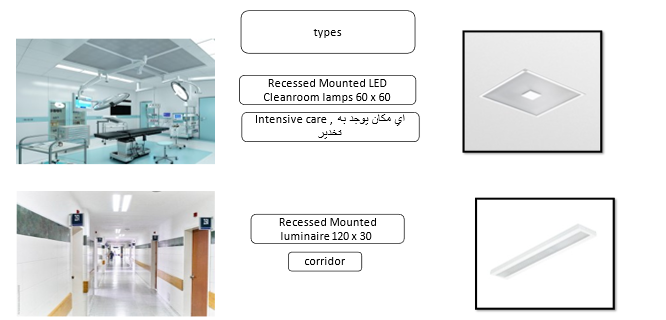
\includegraphics[width=1\linewidth]{f 1.png}
   
    \label{fig:f 1}
\end{figure}
\begin{figure}[!h]
    \centering
    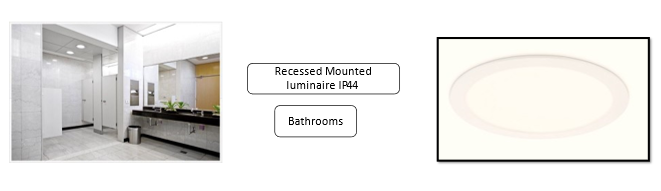
\includegraphics[width=1\linewidth]{f 2.png}
   
    \label{fig:f 2}
\end{figure}
\begin{figure}[!h]
    \centering
    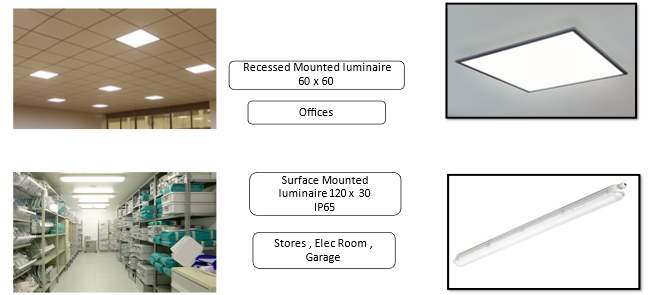
\includegraphics[width=1\linewidth]{f 3.png}
    \caption{types of flashlights and where to use}
  
    \label{fig:f 3}
\end{figure}
\newpage
\\Recessed Mounted luminaire 60 x 60 as shown in Figure \ref{fig:fikry 9}.
\begin{figure}[!h]
    \centering
    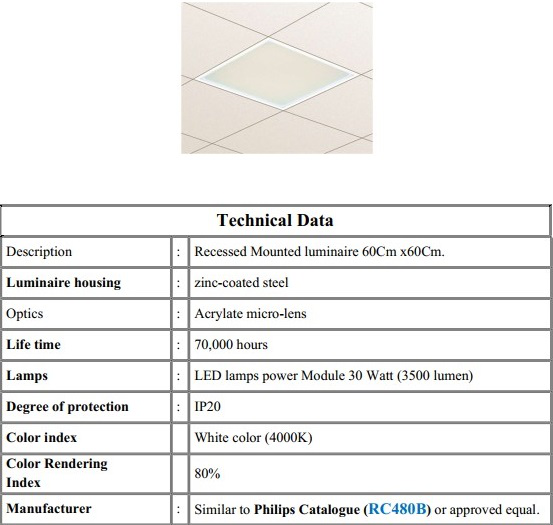
\includegraphics[width=1\linewidth]{fikry 9.png}
    \caption{Recessed Mounted Luminaries 60Cm x 60Cm}
    \label{fig:fikry 9}
\end{figure}
\newpage
\\Surface Mounted Pacific LED Lamps as shown in Figure \ref{fig:fikry 10}.
\begin{figure}[!h]
    \centering
    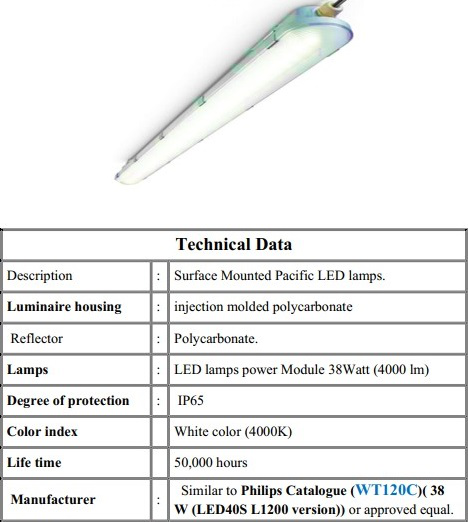
\includegraphics[width=1\linewidth]{fikry 10.png}
    \caption{Surface Mounted Pacific LED Lamps}
    \label{fig:fikry 10}
\end{figure}
\newpage
\\Recessed Mounted LED Cleanroom lamps as shown in Figure \ref{fig:fikry 11}.
\begin{figure}[!h]
    \centering
    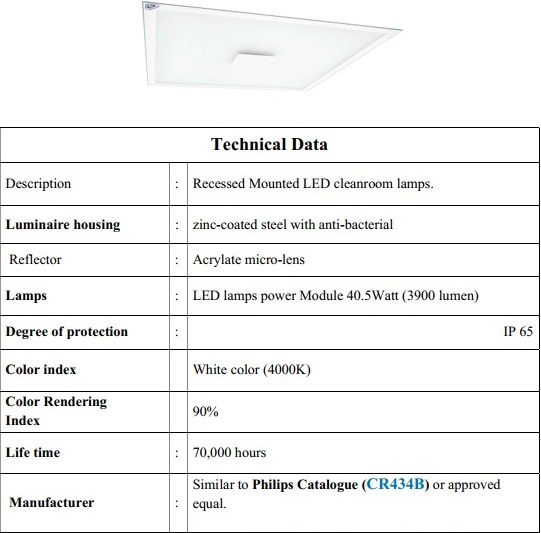
\includegraphics[width=1\linewidth]{fikry 11.png}
    \caption{Recessed Mounted LED cleanroom Lamps}
    \label{fig:fikry 11}
\end{figure}
\newpage
\\Recessed Mounted luminaire 60 x 60 as shown in Figure \ref{fig:fikry 12}.
\begin{figure}[!h]
    \centering
    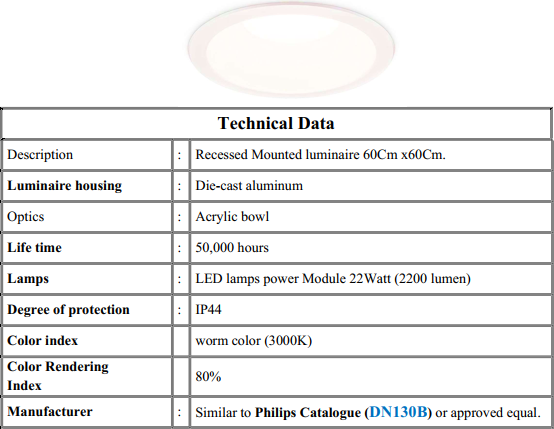
\includegraphics[width=1\linewidth]{fikry 12.png}
    \caption{Recessed Mounted Luminaire 60Cm x 60Cm}
    \label{fig:fikry 12}
\end{figure}
\newpage
\\Recessed Mounted luminaire 60 x 60 as shown in Figure \ref{fig:fikry 13}.
\begin{figure}[!h]
    \centering
    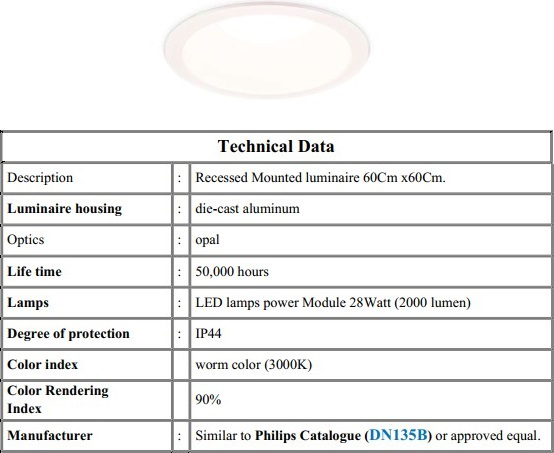
\includegraphics[width=1\linewidth]{fikry 13.png}
    \caption{Recessed Mounted Luminaire 60Cm x 60Cm}
    \label{fig:fikry 13}
\end{figure}
\newpage
\\Recessed Mounted Luminaire 60Cm x 60Cm as shown in Figure \ref{fig:fikry 14}.
\begin{figure}[!h]
    \centering
    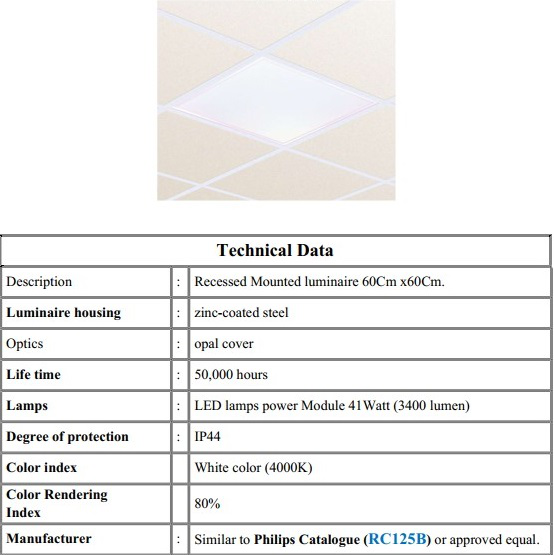
\includegraphics[width=1\linewidth]{fikry 14.png}
    \caption{Recessed Mounted Luminaire 60Cm x 60Cm}
    \label{fig:fikry 14}
\end{figure}
\newpage
\\ Surface Mounted Pacific LED Lamps (60CM) as shown in Figure \ref{fig:fikry 15}.
\begin{figure}[!h]
    \centering
    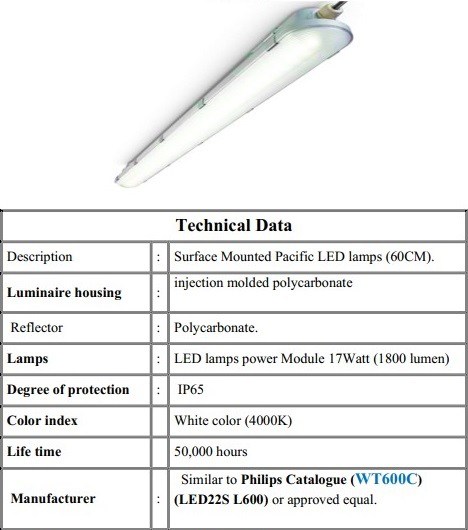
\includegraphics[width=1\linewidth]{fikry 15.png}
    \caption{Surface Mounted Pacific LED Lamps (60CM)}
    \label{fig:fikry 15}
\end{figure}
\newpage
\\Recessed Mounted LED Cleanlamp Lamps as shown in Figure \ref{fig:fikry 16}.
\begin{figure}[!h]
    \centering
    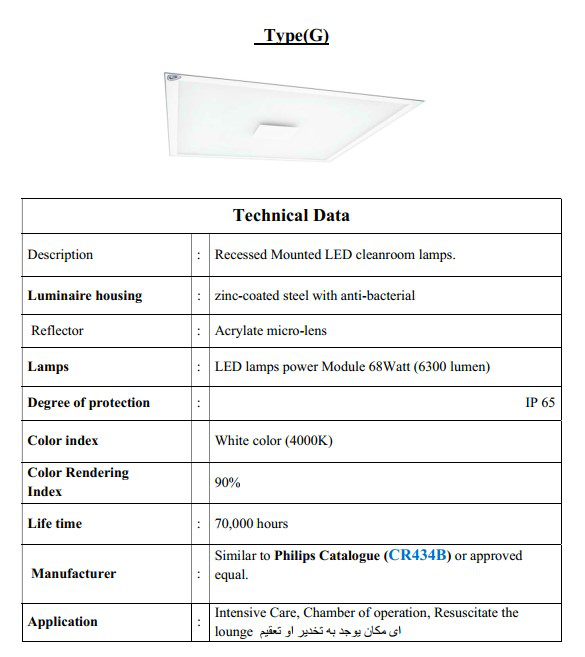
\includegraphics[width=1\linewidth]{fikry 16.png}
    \caption{Recessed Mounted LED Cleanlamp Lamps}
    \label{fig:fikry 16}
\end{figure}
\newpage

\section{Ceiling Type}
\subsection{Surface Mounted ceiling}
\\Surface mount ceiling lights are a vital part of any commercial space and provide the light necessary to create a warm and welcoming environment. Instead of recessing into the ceiling, these fixtures mount directly to any hard ceiling as shown in Figure \ref{fig:fikry 17}.
\begin{figure}[!h]
    \centering
    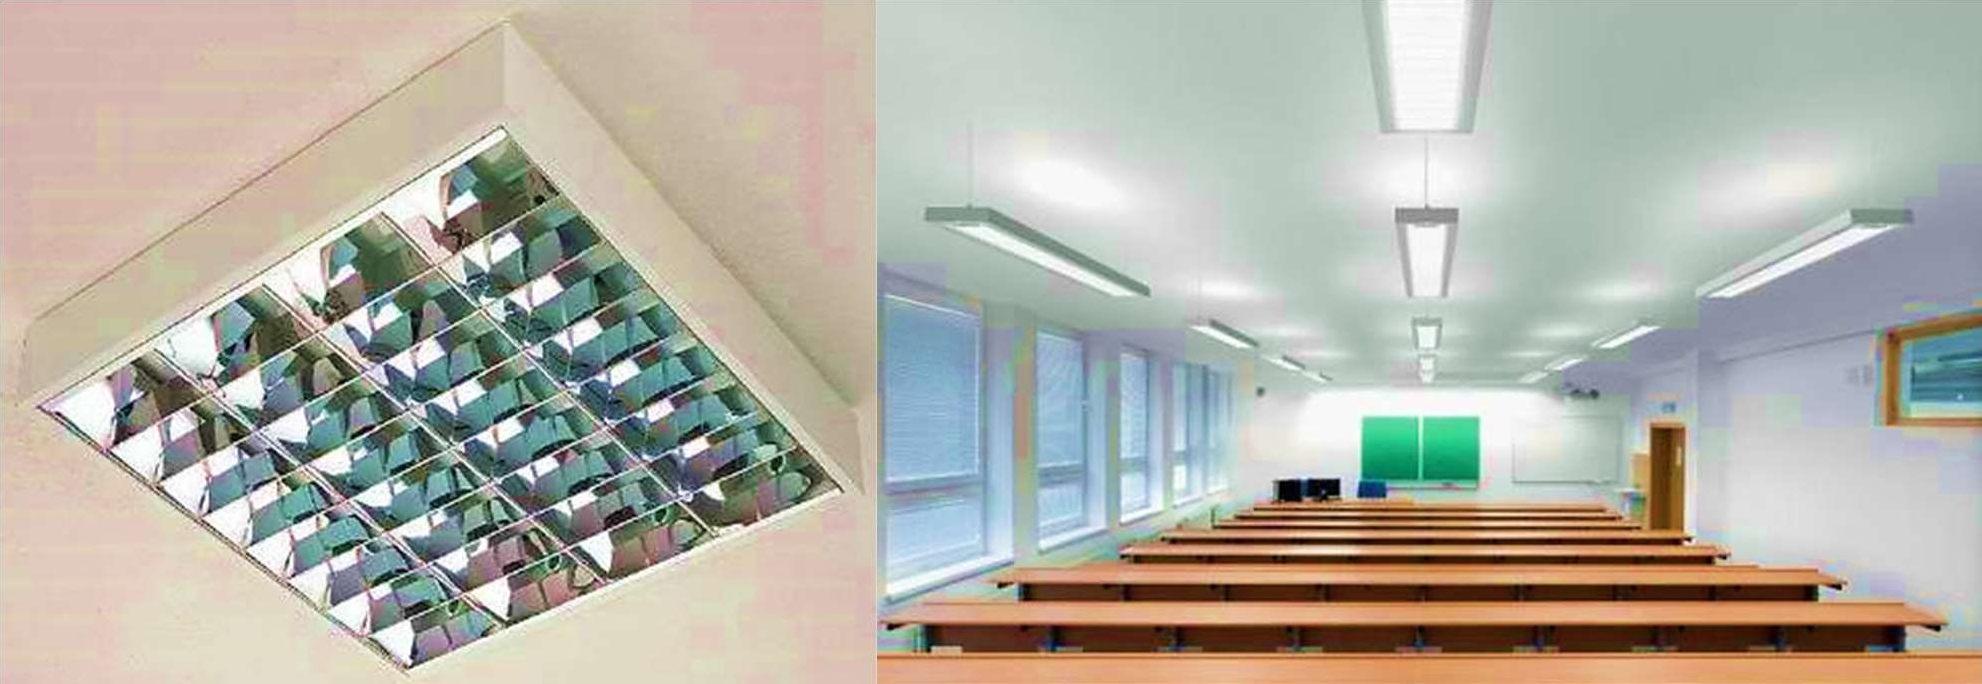
\includegraphics[width=1\linewidth]{fikry 17.png}
    \caption{Surface Mounted Ceiling}
    \label{fig:fikry 17}
\end{figure}
\subsection{Recessed Mounted Ceiling}
A recessed ceiling, also known as a tray ceiling, is created when the central portion of the ceiling is higher than the surrounding area as shown in Figure \ref{fig:fikry 18}.
\begin{figure}[!h]
    \centering
    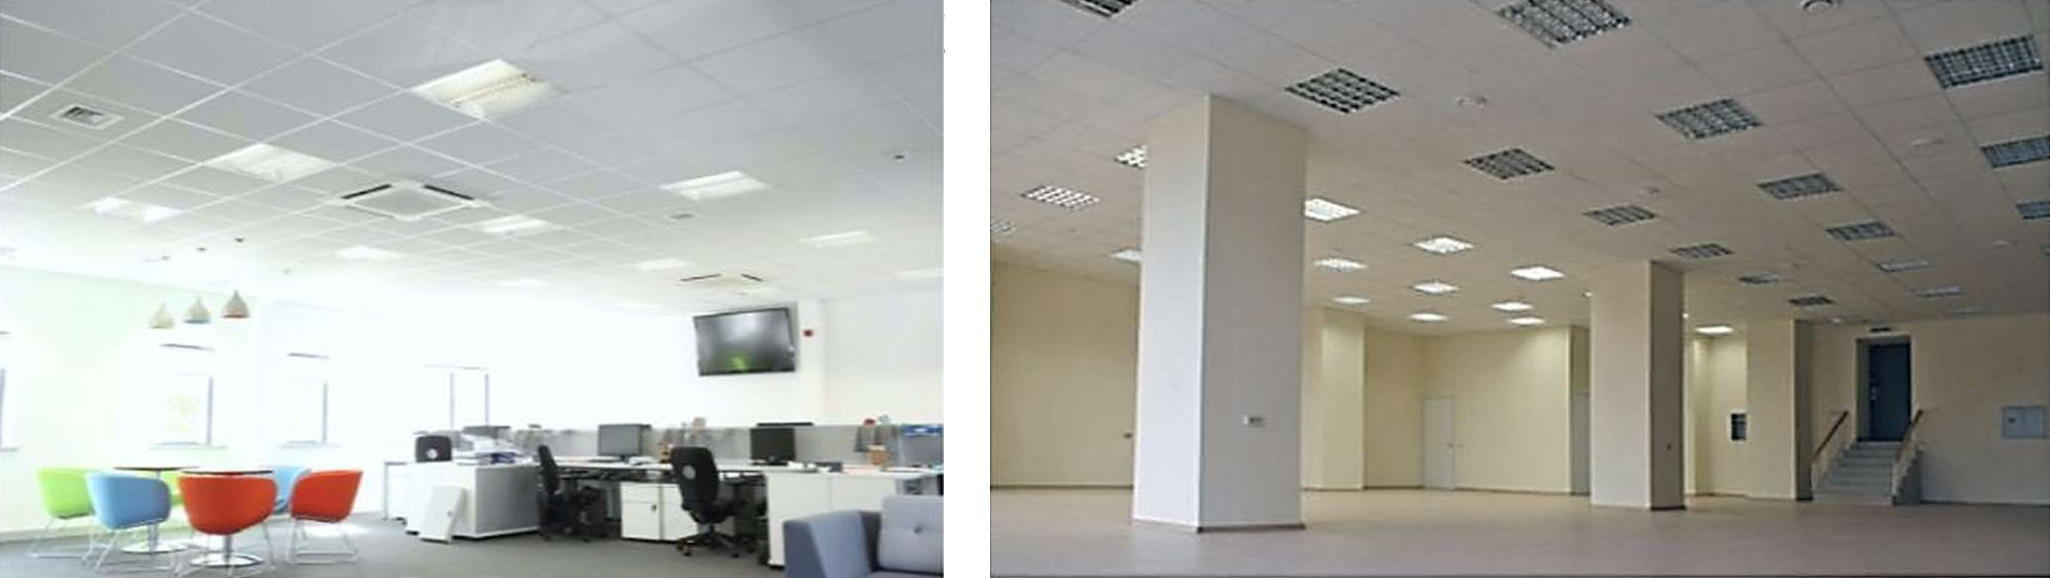
\includegraphics[width=1\linewidth]{fikry 18.png}
    \caption{Recessed Mounted Ceiling}
    \label{fig:fikry 18}
\end{figure}
\subsection{Suspended Mounted Ceiling}
\\ Suspended mounting refers to hang the fixtures from the ceiling or other building structures by cords, chains, straps, rods, wires, etc as shown in Figure \ref{fig:fikry 19}.
\begin{figure}[!h]
    \centering
    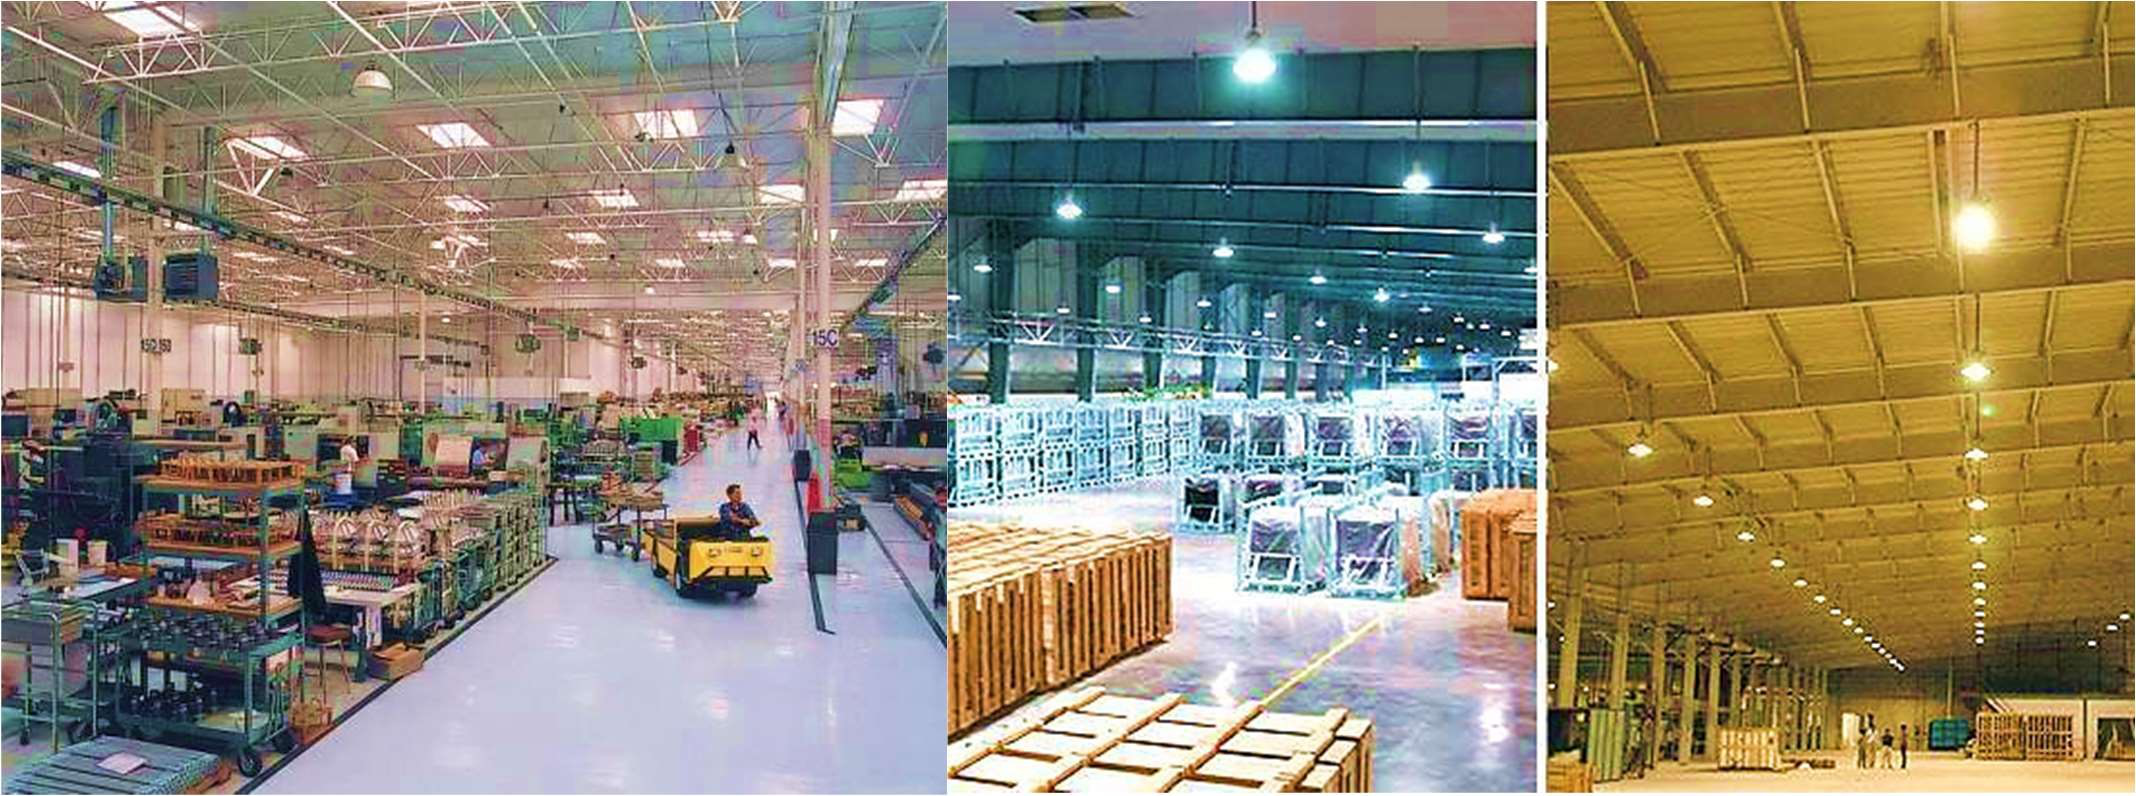
\includegraphics[width=1\linewidth]{fikry 19.png}
    \caption{Suspended Mounted Ceiling}
    \label{fig:fikry 19}
\end{figure}
\newpage
\section{Lighting Lux}
\begin{table}[!h]
\centering
\caption{Lighting LUX of All Rooms in Suez Hospital}
\arrayrulecolor{black}
\begin{tabular}{!{\color{white}\vrule}c!{\color{black}\vrule}c!{\color{white}\vrule}c!{\color{white}\vrule}c!{\color{white}\vrule}c!{\color{white}\vrule}c!{\color{white}\vrule}} 
\hline
\rowcolor[rgb]{0.31,0.506,0.741} \multicolumn{1}{!{\color{white}\vrule}c}{\textbf{\textcolor{white}{NO}}} & \multicolumn{1}{c}{\textbf{\textcolor{white}{Room Function}}} & \textbf{\textcolor{white}{Lux}} & \multicolumn{1}{c}{\textbf{\textcolor{white}{NO}}}                & \multicolumn{1}{c}{\textbf{\textcolor{white}{Room Function}}} & \textbf{\textcolor{white}{LUX}}  \\ 
\hhline{>{\arrayrulecolor{white}}|>{\arrayrulecolor{black}}->{\arrayrulecolor{white}}->{\arrayrulecolor{black}}->{\arrayrulecolor{white}}-->{\arrayrulecolor{black}}->{\arrayrulecolor{white}}|}
\rowcolor[rgb]{0.722,0.8,0.894} {\cellcolor[rgb]{0.31,0.506,0.741}}\textbf{\textcolor{white}{1}}          & ~ ~ ~ ~ ~ ~ ~ ~ ~ Kitchen~ ~ ~ ~ ~ ~ ~ ~ ~ ~\textbf{}         & 500                             & {\cellcolor[rgb]{0.31,0.506,0.741}}\textbf{\textcolor{white}{25}} & ~ ~ ~ ~ ~ ~ ~ ~ Dexa~ ~ ~ ~ ~ ~ ~ ~~                          & 400                              \\ 
\arrayrulecolor{black}\hline
\rowcolor[rgb]{0.859,0.898,0.945} {\cellcolor[rgb]{0.31,0.506,0.741}}\textbf{\textcolor{white}{2}}        & Restaurant\textbf{}                                           & 300                             & {\cellcolor[rgb]{0.31,0.506,0.741}}\textbf{\textcolor{white}{26}} & Equipment’s
  room                                            & 150                              \\ 
\hline
\rowcolor[rgb]{0.722,0.8,0.894} {\cellcolor[rgb]{0.31,0.506,0.741}}\textbf{\textcolor{white}{3}}          & Maintenance room\textbf{}                                     & 150                             & {\cellcolor[rgb]{0.31,0.506,0.741}}\textbf{\textcolor{white}{27}} & Changing
  Room                                               & 150                              \\ 
\hline
\rowcolor[rgb]{0.859,0.898,0.945} {\cellcolor[rgb]{0.31,0.506,0.741}}\textbf{\textcolor{white}{4}}        & Mechanical room\textbf{}                                      & 150                             & {\cellcolor[rgb]{0.31,0.506,0.741}}\textbf{\textcolor{white}{28}} & Nurse station                                                 & 300                              \\ 
\hline
\rowcolor[rgb]{0.722,0.8,0.894} {\cellcolor[rgb]{0.31,0.506,0.741}}\textbf{\textcolor{white}{5}}          & Mortuary\textbf{}                                             & 300                             & {\cellcolor[rgb]{0.31,0.506,0.741}}\textbf{\textcolor{white}{29}} & Store                                                         & 150                              \\ 
\hline
\rowcolor[rgb]{0.859,0.898,0.945} {\cellcolor[rgb]{0.31,0.506,0.741}}\textbf{\textcolor{white}{6}}        & Washing area\textbf{}                                         & 300                             & {\cellcolor[rgb]{0.31,0.506,0.741}}\textbf{\textcolor{white}{30}} & Doctors' Room                                                  & 300                              \\ 
\hline
\rowcolor[rgb]{0.722,0.8,0.894} {\cellcolor[rgb]{0.31,0.506,0.741}}\textbf{\textcolor{white}{7}}          & Waiting area\textbf{}                                         & 300                             & {\cellcolor[rgb]{0.31,0.506,0.741}}\textbf{\textcolor{white}{31}} & Nurse's
  Lounge                                                & 300                              \\ 
\hline
\rowcolor[rgb]{0.859,0.898,0.945} {\cellcolor[rgb]{0.31,0.506,0.741}}\textbf{\textcolor{white}{8}}        & Prayer\textbf{}                                               & 300                             & {\cellcolor[rgb]{0.31,0.506,0.741}}\textbf{\textcolor{white}{32}} & Laboratories                                                  & 500                              \\ 
\hline
\rowcolor[rgb]{0.722,0.8,0.894} {\cellcolor[rgb]{0.31,0.506,0.741}}\textbf{\textcolor{white}{9}}          & Electricity room\textbf{}                                     & 200                             & {\cellcolor[rgb]{0.31,0.506,0.741}}\textbf{\textcolor{white}{33}} & Trauma                                                        & 500                              \\ 
\hline
\rowcolor[rgb]{0.859,0.898,0.945} {\cellcolor[rgb]{0.31,0.506,0.741}}\textbf{\textcolor{white}{10}}       & garage\textbf{}                                               & 150                             & {\cellcolor[rgb]{0.31,0.506,0.741}}\textbf{\textcolor{white}{34}} & Operation
  Room                                              & 500                              \\ 
\hline
\rowcolor[rgb]{0.722,0.8,0.894} {\cellcolor[rgb]{0.31,0.506,0.741}}\textbf{\textcolor{white}{11}}         & Entrance\textbf{}                                             & 300                             & {\cellcolor[rgb]{0.31,0.506,0.741}}\textbf{\textcolor{white}{35}} & Toilets                                                       & 100                              \\ 
\hline
\rowcolor[rgb]{0.859,0.898,0.945} {\cellcolor[rgb]{0.31,0.506,0.741}}\textbf{\textcolor{white}{12}}       & office\textbf{}                                               & 500                             & {\cellcolor[rgb]{0.31,0.506,0.741}}\textbf{\textcolor{white}{36}} & Observation
  Room                                            & 500                              \\ 
\hline
\rowcolor[rgb]{0.722,0.8,0.894} {\cellcolor[rgb]{0.31,0.506,0.741}}\textbf{\textcolor{white}{13}}         & Shop\textbf{}                                                 & 500                             & {\cellcolor[rgb]{0.31,0.506,0.741}}\textbf{\textcolor{white}{37}} & Secretary
  Room                                              & 300                              \\ 
\hline
\rowcolor[rgb]{0.859,0.898,0.945} {\cellcolor[rgb]{0.31,0.506,0.741}}\textbf{\textcolor{white}{14}}       & corridor\textbf{}                                             & 150                             & {\cellcolor[rgb]{0.31,0.506,0.741}}\textbf{\textcolor{white}{38}} & Laundry                                                       & 300                              \\ 
\hline
\rowcolor[rgb]{0.722,0.8,0.894} {\cellcolor[rgb]{0.31,0.506,0.741}}\textbf{\textcolor{white}{15}}         & Treatment Room\textbf{}                                       & 500                             & {\cellcolor[rgb]{0.31,0.506,0.741}}\textbf{\textcolor{white}{39}} & Sterilizers                                                   & 300                              \\ 
\hline
\rowcolor[rgb]{0.859,0.898,0.945} {\cellcolor[rgb]{0.31,0.506,0.741}}\textbf{\textcolor{white}{16}}       & Gym\textbf{}                                                  & 500                             & {\cellcolor[rgb]{0.31,0.506,0.741}}\textbf{\textcolor{white}{40}} & Pharmacy                                                      & 300                              \\ 
\hline
\rowcolor[rgb]{0.722,0.8,0.894} {\cellcolor[rgb]{0.31,0.506,0.741}}\textbf{\textcolor{white}{17}}         & Cat scan\textbf{}                                             & 400                             & {\cellcolor[rgb]{0.31,0.506,0.741}}\textbf{\textcolor{white}{41}} & Patient
  Room                                                & 300                              \\ 
\hline
\rowcolor[rgb]{0.859,0.898,0.945} {\cellcolor[rgb]{0.31,0.506,0.741}}\textbf{\textcolor{white}{18}}       & .M.R.I\textbf{}                                               & 400                             & {\cellcolor[rgb]{0.31,0.506,0.741}}\textbf{\textcolor{white}{42}} & One Day
  Surgery                                             & 500                              \\ 
\hline
\rowcolor[rgb]{0.722,0.8,0.894} {\cellcolor[rgb]{0.31,0.506,0.741}}\textbf{\textcolor{white}{19}}         & X-ray\textbf{}                                                & 400                             & {\cellcolor[rgb]{0.31,0.506,0.741}}\textbf{\textcolor{white}{43}} & I.C.U                                                         & 500                              \\ 
\hline
\rowcolor[rgb]{0.859,0.898,0.945} {\cellcolor[rgb]{0.31,0.506,0.741}}\textbf{\textcolor{white}{20}}       & Sonar\textbf{}                                                & 400                             & {\cellcolor[rgb]{0.31,0.506,0.741}}\textbf{\textcolor{white}{44}} & Catheterization                                               & 500                              \\ 
\hline
\rowcolor[rgb]{0.722,0.8,0.894} {\cellcolor[rgb]{0.31,0.506,0.741}}\textbf{\textcolor{white}{21}}         & Mamo -graph\textbf{}                                          & 400                             & {\cellcolor[rgb]{0.31,0.506,0.741}}\textbf{\textcolor{white}{45}} & Recovery                                                      & 300                              \\ 
\hline
\rowcolor[rgb]{0.859,0.898,0.945} {\cellcolor[rgb]{0.31,0.506,0.741}}\textbf{\textcolor{white}{22}}       & Panorama                                                      & 400                             & {\cellcolor[rgb]{0.31,0.506,0.741}}\textbf{\textcolor{white}{46}} & endoscope                                                     & 500                              \\ 
\hline
\rowcolor[rgb]{0.722,0.8,0.894} {\cellcolor[rgb]{0.31,0.506,0.741}}\textbf{\textcolor{white}{23}}         & .Echo\textbf{}                                                & 400                             & {\cellcolor[rgb]{0.31,0.506,0.741}}\textbf{\textcolor{white}{47}} & Newborn critical care                                         & 500                              \\ 
\hline
\rowcolor[rgb]{0.859,0.898,0.945} {\cellcolor[rgb]{0.31,0.506,0.741}}\textbf{\textcolor{white}{24}}       & Ultrasound\textbf{}                                           & 400                             & {\cellcolor[rgb]{0.31,0.506,0.741}}\textbf{\textcolor{white}{48}} & stroke unite                                                  & 500                              \\
\hline
\end{tabular}
\arrayrulecolor{black}
\end{table}
\section{Lighting Distribution}
\subsection{Types of Calculation}
\begin{enumerate}
    \item Manual
    \\ Using Equation \ref{equation:Manual calculation} to calculation Lumen Manually
    \begin{equation}
        N=\frac{Lux \times a \times b}{Lumen \times U.F \times M.F \times n}
        \label{equation:Manual calculation}
    \end{equation}
    \\ Where:
    \begin{itemize}
        \item $N$ : Number of Luminaries
        \item $n$ : Number of lamps per luminaries
        \item $a$ : Room width
        \item $b$ : Room length
        \item $U.F$ : Utilization factor
        \item $M.F$ : Maintenance factor
        \item $Lux$ : Lighting level, get from standard table (IEC, EC and NEC)
    \end{itemize}
    \\ Use the output of the calculation Excel sheet at Table \ref{tab:Lux Calculation Using Excel sheet}  to distribution Luminaire in AutoCAD as Shown in Figure \ref{fig:fikry 20}
\begin{table}[!h]
\centering
\caption{Lux Calculation Using Excel Sheet}
\label{tab:Lux Calculation Using Excel sheet}
\begin{tabular}{lclllc}
\multicolumn{6}{c}{{\cellcolor[rgb]{0.055,0.337,0.447}}\textcolor{white}{\textbf{LUX CALCULATION}}}                                                                                                                   \\
\multicolumn{2}{l}{{\cellcolor[rgb]{0.078,0.51,0.671}}\textcolor{white}{ Enter the :}} &  &  & \multicolumn{2}{c}{{\cellcolor[rgb]{0.078,0.51,0.671}}\textcolor{white}{result}}                                       \\
{\cellcolor[rgb]{0.467,0.804,0.933}}Length($L)$      & 3                               &  &  & {\cellcolor[rgb]{0.467,0.804,0.933}}$n$                                                & 5                             \\
{\cellcolor[rgb]{0.467,0.804,0.933}}Width($W$)       & 4                               &  &  & {\cellcolor[rgb]{0.467,0.804,0.933}}num of luminaires/row                              & 2                             \\
{\cellcolor[rgb]{0.467,0.804,0.933}}Height($H$)      & 3                               &  &  & {\cellcolor[rgb]{0.467,0.804,0.933}}num of row                                         & 3                             \\
{\cellcolor[rgb]{0.467,0.804,0.933}}$Lumen$(ø)       & 2000                            &  &  & {\cellcolor[rgb]{0.467,0.804,0.933}}spacing in row                                     & 1.5                           \\
{\cellcolor[rgb]{0.467,0.804,0.933}}$Lux $($E$)      & 150                             &  &  & {\cellcolor[rgb]{0.467,0.804,0.933}}space between row                                  & 1.34                          \\
{\cellcolor[rgb]{0.467,0.804,0.933}}$MF$             & 0.5                             &  &  & {\cellcolor[rgb]{0.467,0.804,0.933}}Swall/w                                            & 0.75                          \\
{\cellcolor[rgb]{0.467,0.804,0.933}}Height work plan & 0.8                             &  &  & {\cellcolor[rgb]{0.467,0.804,0.933}}Swall/L                                            & 0.67                          \\
{\cellcolor[rgb]{0.467,0.804,0.933}}$K$              & 0.779220779                     &  &  & {\cellcolor[rgb]{0.467,0.804,0.933}}                                                   & \multirow{4}{*}{\textbf{6 }}  \\
{\cellcolor[rgb]{0.467,0.804,0.933}}$UF$             & 0.6                             &  &  & {\cellcolor[rgb]{0.467,0.804,0.933}}                                                   &                               \\
{\cellcolor[rgb]{0.467,0.804,0.933}}$Nlb$            & 0.6                             &  &  & {\cellcolor[rgb]{0.467,0.804,0.933}}                                                   &                               \\
{\cellcolor[rgb]{0.467,0.804,0.933}}$SHR$            &                                 &  &  & \multirow{-4}{*}{{\cellcolor[rgb]{0.467,0.804,0.933}}\textbf{Numer of lumniers($N$) }} &                              
\end{tabular}
\end{table}
\begin{figure}[!h]
    \centering
    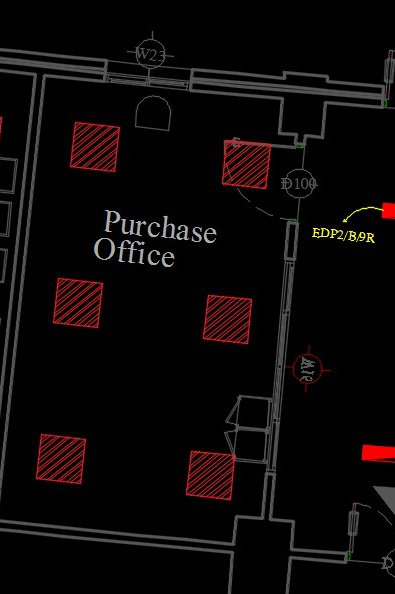
\includegraphics[width=0.4\linewidth]{fikry 20.png}
    \caption{Purchase Office Lighting Form}
    \label{fig:fikry 20}
\end{figure}
\\
\\
\item Programming Distribution using (DIALux program)
\\This Program is mainly used to get Number of Luminaries in a Place, Its type and type of Lamps as shown in figure \ref{fig:fikry 21}.
\\ \textbf{After Installing the program, it can be found that:}
\begin{itemize}
    \item Blue Icon for Light Wizard
    \item Red Icon Real Project
\end{itemize}
\begin{figure}[!h]
    \centering
    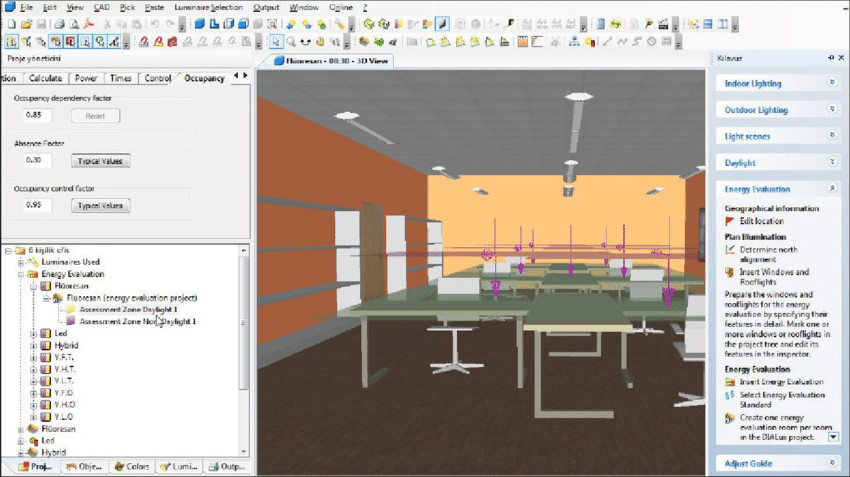
\includegraphics[width=1\linewidth]{fikry 21.png}
    \caption{DIALux Program Screen}
    \label{fig:fikry 21}
\end{figure}
\textbf{Choose type of lighting}
\\ Guide menu > Load DWG or DXF File.
\\ Take into Consideration the Units used in CAD File.
\\ When you Finish Inserting the CAD File you will see nothing changed!! And so insert new Room to see the Drawing.
\\ When the Drawing appears, Start inserting new Rooms.
\\ Guide menu > Insert New Room.
\\ \textbf{To Edit the Room shape:}
\begin{itemize}
    \item Right click on the room > Edit Room Geometry
    \item Move each point individually
    \item OR right click > Draw Rectangle then select type of luminaire as shown in figure \ref{fig:fikry 22} \& \ref{fig:fikry 23}
\end{itemize}
\begin{figure}[!h]
    \centering
    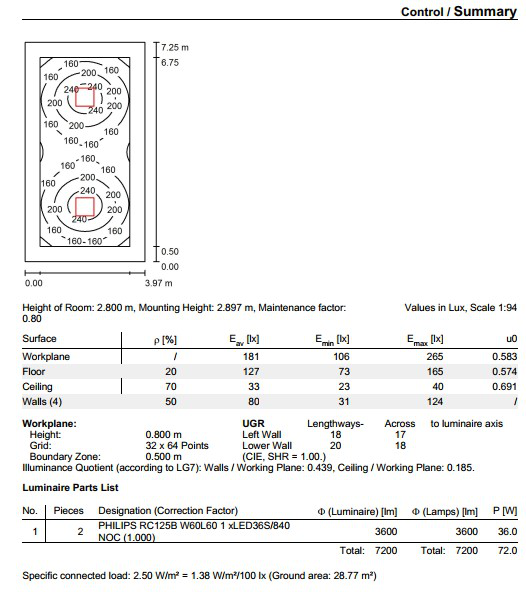
\includegraphics[width=0.5\linewidth]{fikry 22.png}
    \caption{DIALux Output Sheet For Control Room}
    \label{fig:fikry 22}
\end{figure}
\begin{figure}[!h]
    \centering
    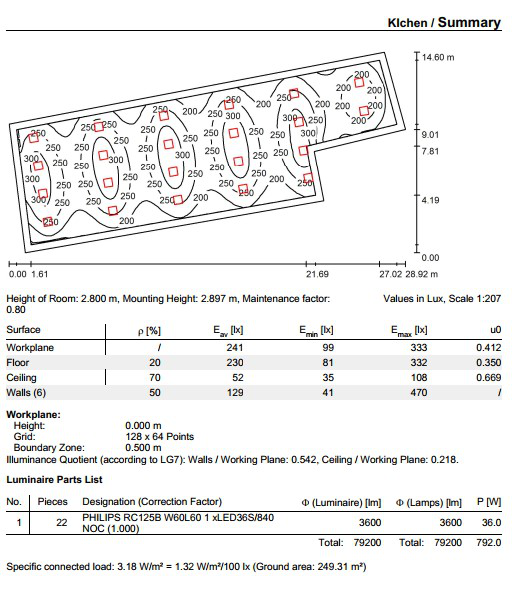
\includegraphics[width=0.5\linewidth]{fikry 23.png}
    \caption{DIALux Output Sheet For Kitchen}
    \label{fig:fikry 23}
\end{figure}
\end{enumerate}
\newpage
\section{Light Distribution design \& Shop Drawing  in this work}
\subsection{Design}
\\Electrical design entails planning, creating, testing, or supervising the development and installation of electrical equipment, including lighting equipment, power systems, power distribution, fire and life safety systems, electronic components, and voice and data communications infrastructure as shown in figure \ref{fig:fikry 24}

    \begin{figure}[!h]
    \centering
    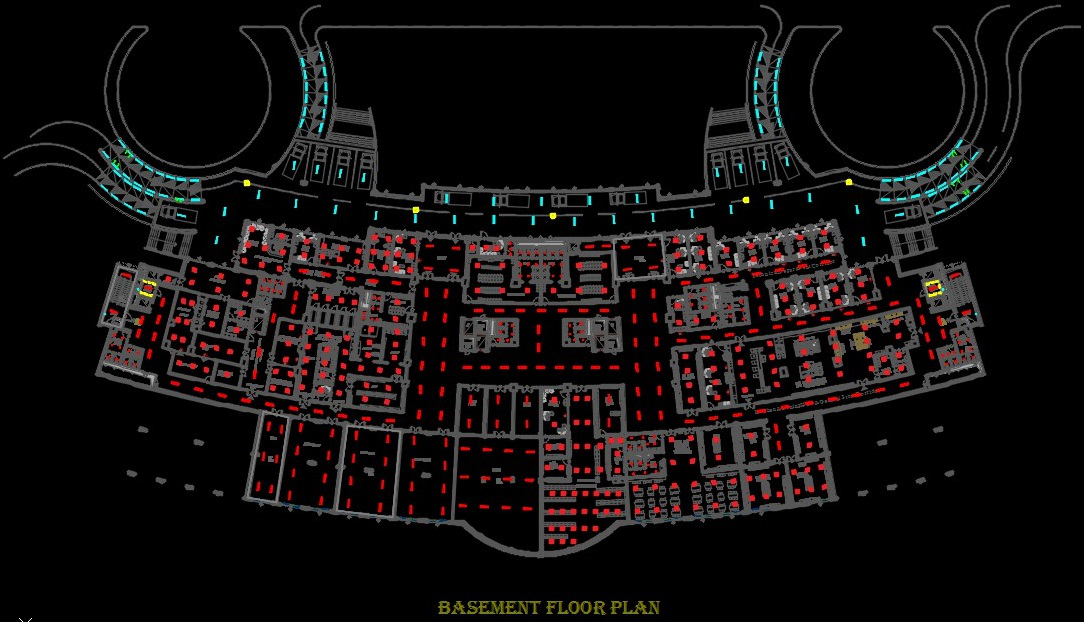
\includegraphics[width=1\linewidth]{fikry 24.png}
    \caption{Sample of Lighting Distribution}
    \label{fig:fikry 24}
\end{figure}
\newpage
\\ lighting design sample  as shown in Figures \ref{fig:f 4} \& \ref{fig:f 5}
  \begin{figure}[!h]
    \centering
    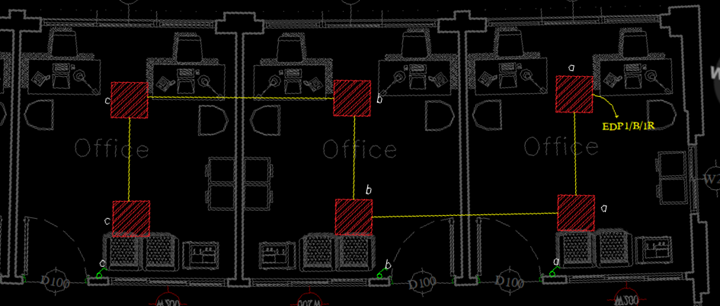
\includegraphics[width=1\linewidth]{f 4.png}
    \caption{Sample of Design}
    \label{fig:f 4}
\end{figure}
  \begin{figure}[!h]
    \centering
    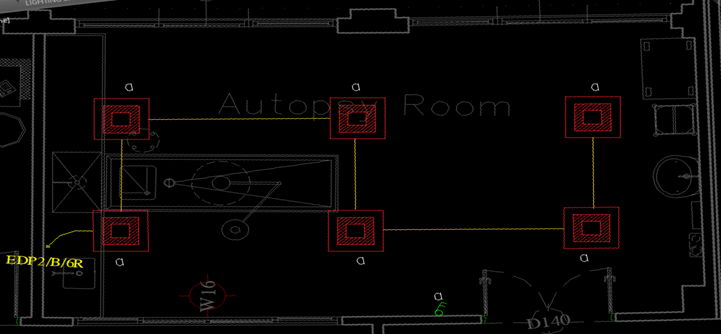
\includegraphics[width=1\linewidth]{f 5.png}
    \caption{Sample of Design}
    \label{fig:f 5}
\end{figure}





\newpage
\subsection{Shop Drawing}
\\Shop drawings thus produced are used by trade contractors to prefabricate the electrical assemblies and subsequently install them at site. We provide exact dimensions of electrical equipment, accurate layout details to make installations run smoothly as shown in figure \ref{fig:fikry 25}
   
      \begin{figure}[!h]
    \centering
    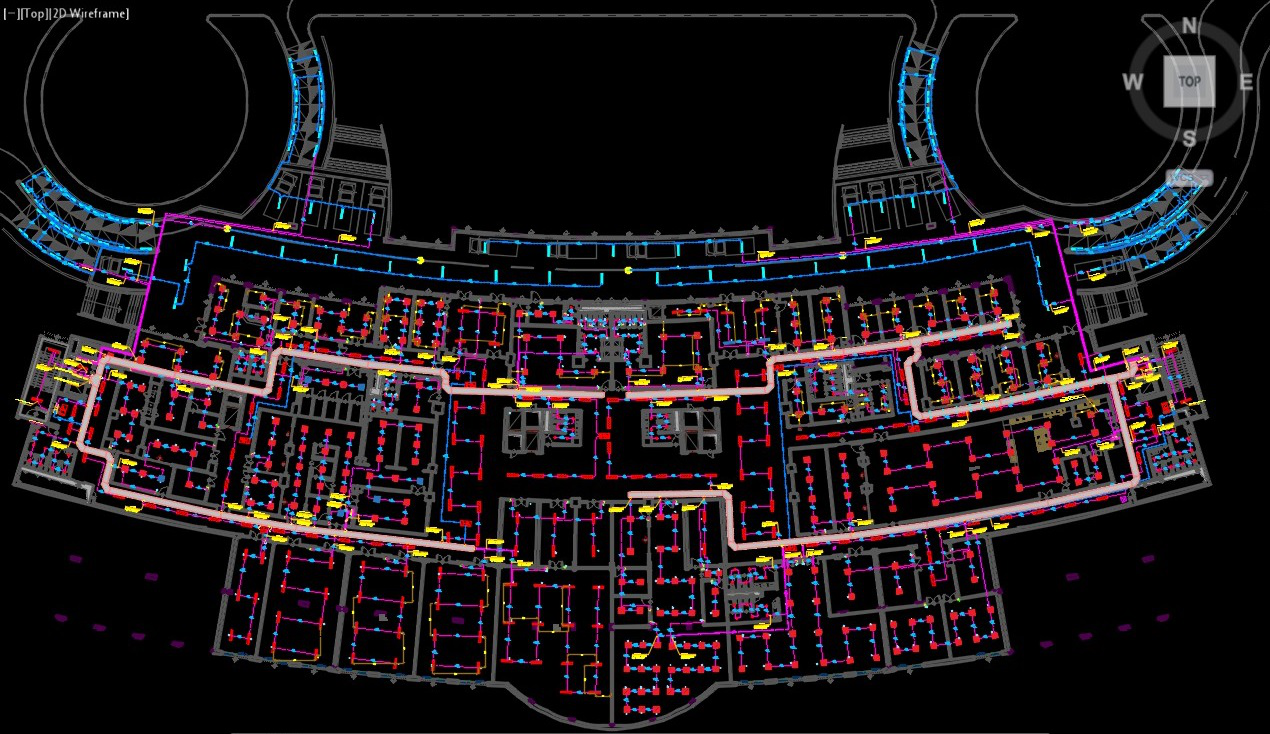
\includegraphics[width=1\linewidth]{fikry 25.png}
    \caption{Sample of Shop Drawing Design}
    \label{fig:fikry 25}
\end{figure}
\newpage
\\lighting shop drawing sample as shown in Figures \ref{fig:f 6} \& \ref{fig:f 7}
  \begin{figure}[!h]
    \centering
    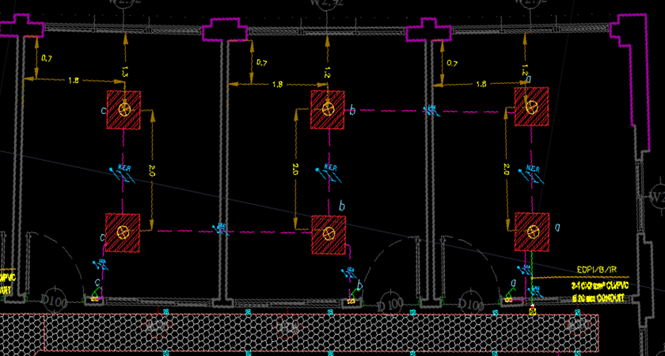
\includegraphics[width=1\linewidth]{f 6.png}
    \caption{Sample of Shop Drawing Design}
    \label{fig:f 6}
\end{figure}
  \begin{figure}[!h]
    \centering
    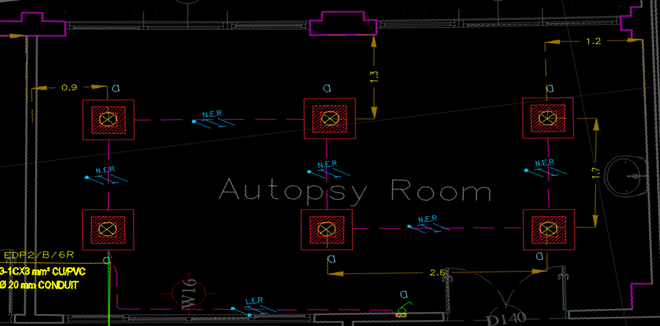
\includegraphics[width=1\linewidth]{f 7.png}
    \caption{Sample of Shop Drawing Design}
    \label{fig:f 7}
\end{figure}
\subsubsection{Exit Sign }
\\An exit sign is a pictogram or short text in a public facility (such as a building, aircraft, or boat) denoting the location of the closest emergency exit to be used in case of fire or other emergency that requires rapid evacuation as shown in figure \ref{fig:f 8}.
\begin{figure}[!h]
    \centering
    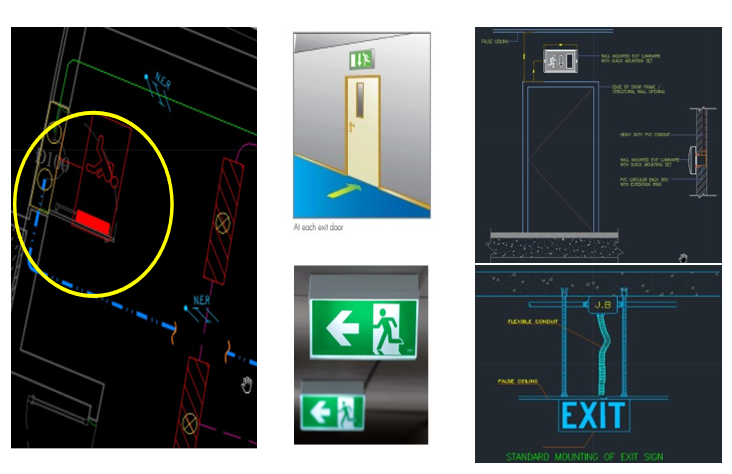
\includegraphics[width=1\linewidth]{f 8.png}
    \caption{Sample Exit Sign}
    \label{fig:f 8}
\end{figure}
\subsubsection{Public car parks (indoor ) }
\\Generally, 250-300 lux light level is sufficient at the entrance and the exit sections of the indoor parkings. At the other sections, 75 lux light level is sufficient. Although it is indoor lighting, it is required minimum IP65 protection class for lighting fixtures which are used in indoor parkings s shown in figure \ref{fig:f 9}. 
\begin{figure}[!h]
    \centering
    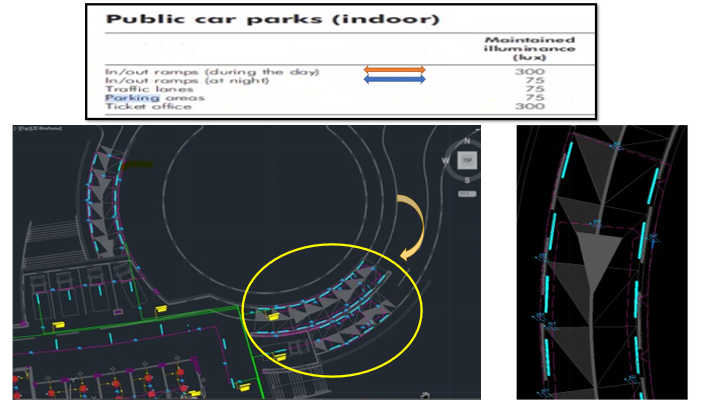
\includegraphics[width=1\linewidth]{f 9.png}
    \caption{Sample Public Car Parks}
    \label{fig:f 9}
\end{figure}



%----------------------------------------------------------------------------------------
%	chapter mahmoud hamdy
%----------------------------------------------------------------------------------------
%%%%%%%%%%%%
\part {Electrical Socket}

\chapter{Electrical Socket}

\chapterimage{socket.png} % Chapter heading image
\section {Types of sockets in hospital}
\begin{enumerate}
    \item Normal sockets
    \\Standard rating for single socket:
    \begin{itemize}
        \item V = 250 volt ; I = 10 A or I = 16 A
    \end{itemize}
    \\S (VA) = according to codes
    \begin{itemize}
        \item  ICE = 180 VA
        \item EC = 250 VA
    \end{itemize}
    \\The shape of normal socket in actually as shown in Figure \ref{fig:s 1}
       \begin{figure}[h!]
    \centering
    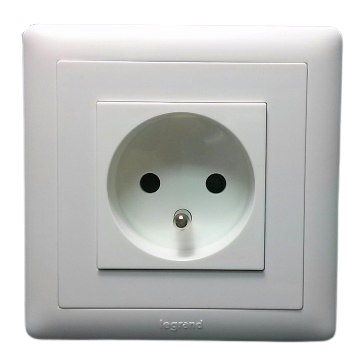
\includegraphics[width=0.3\linewidth]{s 1.png}
    \caption{Single Socket  }
    \label{fig:s 1}
\end{figure}


\newpage
    \item Double Sockets 
    \\Standard rating for double socket:
    \begin{itemize}
        \item V = 250 volt ; I = 10 A or16 A
    \end{itemize}
    \\S (VA) = according to codes
    \begin{itemize}
        \item  ICE = 360 VA
        \item EC = 500 VA
        \\One of the shape of double socket in actually as shown in  Figure \ref{fig:s 2}
    \end{itemize}
       \begin{figure}[h!]
    \centering
    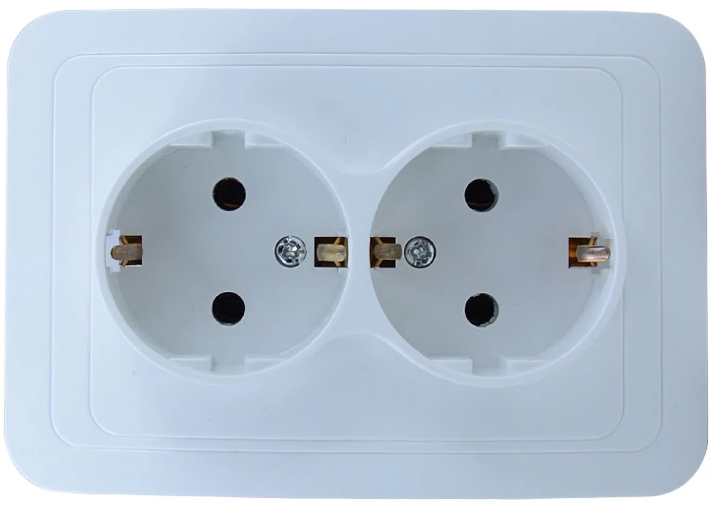
\includegraphics[width=0.7\linewidth]{s 2.png}
    \caption{   Double Socket  }
    \label{fig:s 2}
\end{figure}
    
    
    \item  Power socket
    \\Standard rating for power socket:
    \begin{itemize}
        \item V = 250 volt ;  I = 20 A or 32 A
         \item For (500 < S > 3000 VA) ↔ Take 20A.
 \item For (3000 < S > 5000 VA) ↔ Take 32A.
 \item Take it in calculation (Depend on load) For application above 5 kva.
    \end{itemize}
    \\Application:
    \begin{enumerate}
        \item Kitchen 
        \item Bath Rooms (heater and hand drier)
        \item Laundry
        \item Drilling Machines
  
    \end{enumerate}
    \\The power socket as like as the normal socket but it can loaded more ,One of the shape of power socket in actually as shown in  Figure \ref{fig:s 3}
    \begin{figure}[h!]
    \centering
    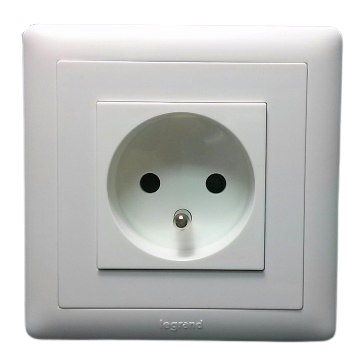
\includegraphics[width=0.4\linewidth]{s 3.png}
    \caption{   Power Socket  }
    \label{fig:s 3}
\end{figure}


    \item U.P.S socket
    \\ Standard rating for U.P.S Sockets: 
    \begin{itemize}
        \item  V = 250 volt; I = 10 A or 16 A
        \item Take it in calculation (Depend on load).  \item A separated distribution board For UPS- socket should be design.

\end{itemize}
\\It used with loads that should not disconnected ,One of the shape of ups socket in actually as shown in  Figure \ref{fig:s 4}
\begin{figure}[h!]
    \centering
    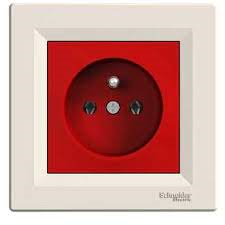
\includegraphics[width=0.5\linewidth]{s 4.png}
    \caption{   U.P.S Socket  }
    \label{fig:s 4}
\end{figure}

    
    
    \item Weather proof socket
    \\It is normal socket with cover.
     \\Application:
    \begin{enumerate}
        \item Corridors 
        \item Kitchen
        \item Bath Room
        \item Outdoor
        \item Stores
        \item Factories
    \end{enumerate}
    \\ The legand of power as shown in Figure \ref{fig:s 5}
    \begin{figure}[h!]
    \centering
    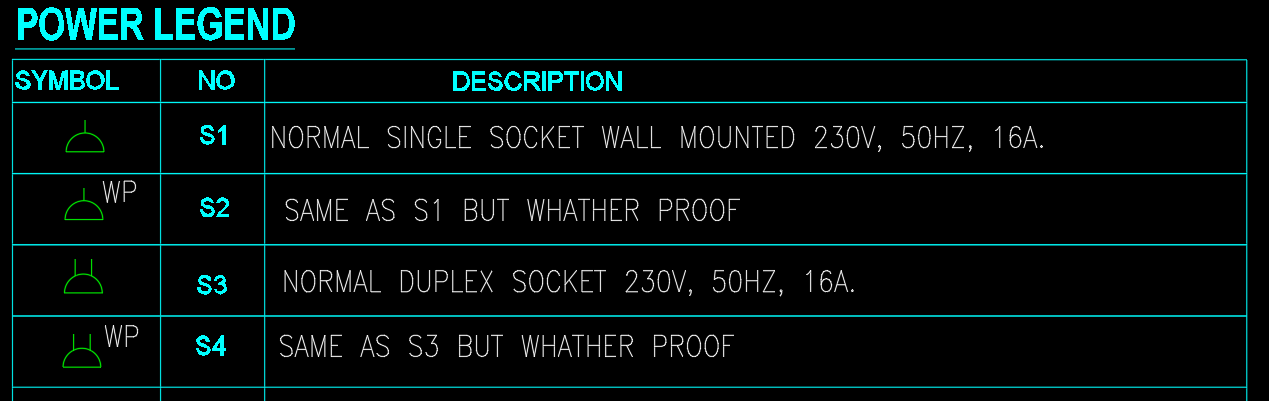
\includegraphics[width=0.8\linewidth]{s 5.png}
    \caption{  Symbol of Weather Proof Sockets}
    \label{fig:s 5}
\end{figure}


    \item Column sockets
    \\ It is used in administrative places.
    \\ Standard rating for column sockets:
    
     \begin{itemize}
        \item  V = 250 V I = 20 A \& Outlet: 6, 12, 18, 24 outlets

\end{itemize}
\\One of the shape of column socket in actually as shown in Figure \ref{fig:s 6}
    \begin{figure}[h!]
    \centering
    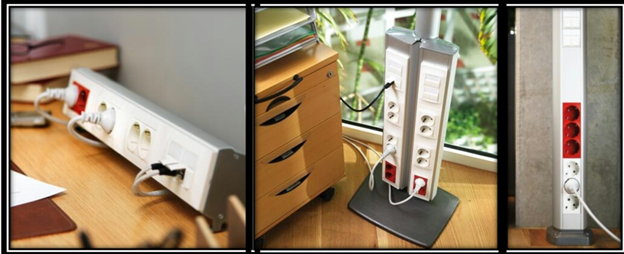
\includegraphics[width=0.8\linewidth]{s 6.png}
    \caption{  Symbol of Column sockets}
    \label{fig:s 6}
\end{figure}

    \item Trunking Socket
    
\\ It is used in intensive care and recovery rooms.

\\ V = 250 V & I = 20 A & Outlet: 6, 12, and 18
\\the shape of trunking socket in actually  as shown in Figure \ref{fig:s 7}
\begin{figure}[h!]
    \centering
    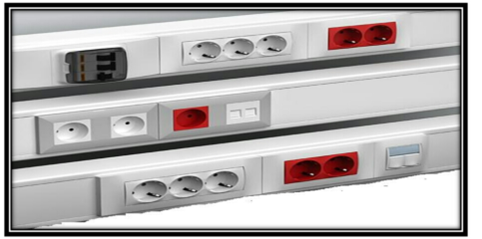
\includegraphics[width=0.8\linewidth]{s 7.png}
    \caption{  Trunking Socket  }
    \label{fig:s 7}
\end{figure}
\\It used in the bed in the patient room as shown in Figure \ref{fig:s 10}
\begin{figure}[h!]
    \centering
    \includegraphics[width=0.7\linewidth]{s 10.png}
    \caption{  Sample From AutoCAD  }
    \label{fig:s 10}
\end{figure}

    \item Floor box 
    \\ V = 250 V \& I = 16 A \& Outlet: 1, 2, 3,4,5,6 \& (IP67)
    \\ the shape of floor box socket in actually as shown in  Figure \ref{fig:s 8}
    \begin{figure}[h!]
    \centering
    \includegraphics[width=0.7\linewidth]{s 8.png}
    \caption{  Floor Boxes  }
    \label{fig:s 8}
\end{figure}
\\ The floor box is used in office as shown in Figure \ref{fig:s 11}
\begin{figure}[h!]
    \centering
    \includegraphics[width=0.7\linewidth]{s 11.png}
    \caption{  Sample From Floor Boxes in AutoCAD }
    \label{fig:s 11}
\end{figure}
  
\end{enumerate}
\newpage
\section{Kitchen load}
\begin{table}[h!]
\centering
\caption{Machine Kitchen Equipment}
\label{tab:machine kitchen equipment}
\arrayrulecolor{black}
\begin{tabular}{!{\color[rgb]{0.557,0.667,0.859}\vrule}l!{\color{black}\vrule}l!{\color[rgb]{0.557,0.667,0.859}\vrule}l!{\color[rgb]{0.557,0.667,0.859}\vrule}} 
\hline
\rowcolor[rgb]{0.267,0.447,0.769} \multicolumn{1}{!{\color[rgb]{0.267,0.447,0.769}\vrule}l}{\textbf{EQUIPMENT}} & \multicolumn{1}{l}{\textbf{\textcolor{white}{KW}}} & \multicolumn{1}{l!{\color[rgb]{0.267,0.447,0.769}\vrule}}{\textbf{PHASE\textcolor{white}{}}}  \\ 
\hhline{>{\arrayrulecolor[rgb]{0.557,0.667,0.859}}|>{\arrayrulecolor{black}}->{\arrayrulecolor[rgb]{0.267,0.447,0.769}}->{\arrayrulecolor{black}}->{\arrayrulecolor[rgb]{0.557,0.667,0.859}}|}
\rowcolor[rgb]{0.851,0.886,0.953} \textbf{DISH WASHING M/C}                                                     & 2                                                  & 1 Ph                                                                                          \\ 
\arrayrulecolor{black}\hline
\textbf{MEAT SLICER}                                                                                            & 0.5                                                & 1 Ph                                                                                          \\ 
\hline
\rowcolor[rgb]{0.851,0.886,0.953} \textbf{OVEN}                                                                 & 7                                                  & 3 Ph                                                                                          \\ 
\hline
\textbf{GRILL}                                                                                                  & 6                                                  & 3 Ph                                                                                          \\ 
\hline
\rowcolor[rgb]{0.851,0.886,0.953} \textbf{BOILER}                                                               & 1.8                                                & 1 Ph                                                                                          \\ 
\hline
\textbf{COFFEE MACHINE}                                                                                         & 2.5                                                & 1 Ph                                                                                          \\ 
\hline
\rowcolor[rgb]{0.851,0.886,0.953} \textbf{FRYING}                                                               & 3                                                  & 3Ph                                                                                           \\
\hline
\end{tabular}
\arrayrulecolor{black}
\end{table}

\section{Socket mounting}
\begin{enumerate}
    \item  The level of installation of sockets shall be from 30 cm to 40 cm from the end floor in residential places and offices, except for kitchens and bathrooms, so they shall be at a level from 1.20 m to 1.35 m according to the Egyptian code.
    \item The socket must be equipped with a means that touches the ground in the     body of the metal case in which it is installed.
    \item The face of the socket box shall be made of a solid insulating material that is not flammable and does not soften when its temperature rises to 58°C, and it must not be deformed or dented during normal use.
    \item The single or double sockets must be of the bipolar type and the earthed pole. 
    \item The rated value of current and voltage must be indicated or illustrated on the sockets in bold letters.
    \item It is taken into account that the sockets installed in the floors are of a water-resistant type to ensure that they do not result in any danger or damage to the insulation when washing the floors.
    \item It should be taken into account that the sockets installed outside the building are of the water-proof type, whether outside or inside the wall, and fitted with a tight cover to prevent rain water from reaching the electrodes. 
    \item When using sockets or a strong socket on either side of a wall, a horizontal distance should be left in it. At least 083 mm between them to avoid sound transmission through them .
    \item Sockets in bathrooms, kitchens or the like should be in places where they are not within the reach of the arm of a person wet with water. 
    \item  Care must be taken to choose the appropriate degree of protection for the sockets in places exposed to water or dust .
    \item It is not allowed to have sockets in the bathtubs and shower cabins.
    \item The horizontal distance between the outlet of the socket and the vertical wall shall not be more than 1.8 m and between the outlet of the socket that follows it .
\end{enumerate}

\\The distance  between socket at mounting according the Egyptian code  as shown in  Figure \ref{fig:s 9}
\begin{figure}[h!]
    \centering
    \includegraphics[width=1\linewidth]{s 9.png}
    \caption{ The Dimension Between Sockets }
    \label{fig:s 9}
\end{figure}
\newpage
\section{Load of panels}
\begin{enumerate}
    \item normal panels
    \begin{table}[h!]
\centering
\caption{Loads of Normal Panel}
\label{tab:loads of normal panel}
\arrayrulecolor{black}
\begin{tabular}{!{\color[rgb]{0.557,0.667,0.859}\vrule}l!{\color{black}\vrule}l!{\color[rgb]{0.557,0.667,0.859}\vrule}} 
\hline
\rowcolor[rgb]{0.267,0.447,0.769} \multicolumn{1}{!{\color[rgb]{0.267,0.447,0.769}\vrule}l}{\textbf{\textcolor{white}{panel}}} & \multicolumn{1}{l!{\color[rgb]{0.267,0.447,0.769}\vrule}}{\textbf{\textcolor{white}{Load (KVA)}}}  \\ 
\hline
\rowcolor[rgb]{0.851,0.886,0.953} \textbf{PPB1}                                                                                & 32.25                                                                                              \\ 
\hline
\textbf{PPB2}                                                                                                                  & 28.25                                                                                              \\ 
\hline
\rowcolor[rgb]{0.851,0.886,0.953} \textbf{PPB3}                                                                                & 41.85                                                                                              \\ 
\hline
\textbf{PPB4}                                                                                                                  & 30                                                                                                 \\ 
\hline
\rowcolor[rgb]{0.851,0.886,0.953} \textbf{PPB5}                                                                                & 47.52                                                                                              \\ 
\hline
\textbf{PPB6}                                                                                                                  & 52.02                                                                                              \\ 
\hline
\rowcolor[rgb]{0.851,0.886,0.953} \textbf{PPB7}                                                                                & 41.08                                                                                              \\ 
\hline
\textbf{PPB8}                                                                                                                  & 41.1                                                                                               \\ 
\hline
\rowcolor[rgb]{0.851,0.886,0.953} \textbf{PPB9}                                                                                & 70.20                                                                                              \\ 
\hline
\textbf{PPB10}                                                                                                                 & 73.65                                                                                              \\ 
\hline
\rowcolor[rgb]{0.851,0.886,0.953} \textbf{PPB11}                                                                               & 48.88                                                                                              \\ 
\hline
\textbf{PPB12}                                                                                                                 & 38.44                                                                                              \\ 
\hline
\rowcolor[rgb]{0.851,0.886,0.953} \textbf{PPB13}                                                                               & 33.5                                                                                               \\ 
\hline
\textbf{PPB14}                                                                                                                 & 33.5                                                                                               \\ 
\hline
\rowcolor[rgb]{0.851,0.886,0.953} \textbf{TOTAL}                                                                               & 612.24                                                                                             \\
\hline
\end{tabular}
\arrayrulecolor{black}
\end{table}
\newpage
     \item emergancy panals
     
     \begin{table}[h!]
\centering
\caption{Loads of Emergency Panels}
\label{tab:loads of emergency panels}
\arrayrulecolor{black}
\begin{tabular}{!{\color[rgb]{0.557,0.667,0.859}\vrule}l!{\color{black}\vrule}l!{\color[rgb]{0.557,0.667,0.859}\vrule}} 
\hline
\rowcolor[rgb]{0.267,0.447,0.769} \multicolumn{1}{!{\color[rgb]{0.267,0.447,0.769}\vrule}l}{\textbf{\textcolor{white}{panel}}} & \multicolumn{1}{l!{\color[rgb]{0.267,0.447,0.769}\vrule}}{\textbf{\textcolor{white}{Load (KVA)}}}  \\ 
\hline
\rowcolor[rgb]{0.851,0.886,0.953} \textbf{EPPB 1}                                                                              & 7.25                                                                                               \\ 
\hline
\textbf{EPPB 2}                                                                                                                & 37.92                                                                                              \\ 
\hline
\rowcolor[rgb]{0.851,0.886,0.953} \textbf{EPPB 3}                                                                              & 12.72                                                                                              \\ 
\hline
\textbf{EPPB 4}                                                                                                                & 18.12                                                                                              \\ 
\hline
\rowcolor[rgb]{0.851,0.886,0.953} \textbf{EPPB 5}                                                                              & 18.9                                                                                               \\ 
\hline
\textbf{EPPB 6}                                                                                                                & 15.26                                                                                              \\ 
\hline
\rowcolor[rgb]{0.851,0.886,0.953} \textbf{EPPB 7}                                                                              & 16.8                                                                                               \\ 
\hline
\textbf{EPPB 8}                                                                                                                & 14.4                                                                                               \\ 
\hline
\rowcolor[rgb]{0.851,0.886,0.953} \textbf{EPPB 9}                                                                              & 7.5                                                                                                \\ 
\hline
\textbf{EPPB 10}                                                                                                               & 20.20                                                                                              \\ 
\hline
\rowcolor[rgb]{0.851,0.886,0.953} \textbf{EPPB 11}                                                                             & 13.64                                                                                              \\ 
\hline
\textbf{EPPB 12}                                                                                                               & 11.44                                                                                              \\ 
\hline
\rowcolor[rgb]{0.851,0.886,0.953} \textbf{TOTAL}                                                                               & 194.15                                                                                             \\
\hline
\end{tabular}
\arrayrulecolor{black}
\end{table}


      \item U.P.S panels
      \begin{table}[h!]
\centering
\caption{Loads of U.P.S panels}
\label{tab:loads of ups panels}
\arrayrulecolor{black}
\begin{tabular}{!{\color[rgb]{0.557,0.667,0.859}\vrule}l!{\color{black}\vrule}l!{\color[rgb]{0.557,0.667,0.859}\vrule}} 
\hline
\rowcolor[rgb]{0.267,0.447,0.769} \multicolumn{1}{!{\color[rgb]{0.267,0.447,0.769}\vrule}l}{\textbf{\textcolor{white}{Panel}\textcolor{white}{}}} & \multicolumn{1}{l!{\color[rgb]{0.267,0.447,0.769}\vrule}}{\textbf{\textcolor{white}{Load (KVA)}\textcolor{white}{}}}  \\ 
\hline
\rowcolor[rgb]{0.851,0.886,0.953} \textbf{UPPB 1}                                                                                                 & 9.5                                                                                                                   \\ 
\hline
\textbf{UPPB 3}                                                                                                                                   & 19                                                                                                                    \\ 
\hline
\rowcolor[rgb]{0.851,0.886,0.953} \textbf{UPPB 4}                                                                                                 & 19.08                                                                                                                 \\ 
\hline
\textbf{UPPB 5}                                                                                                                                   & 11.68                                                                                                                 \\ 
\hline
\rowcolor[rgb]{0.851,0.886,0.953} \textbf{UPPB 6}                                                                                                 & 11.34                                                                                                                 \\ 
\hline
\textbf{UPPB 7}                                                                                                                                   & 22.4                                                                                                                  \\ 
\hline
\rowcolor[rgb]{0.851,0.886,0.953} \textbf{UPPB 8}                                                                                                 & 20.80                                                                                                                 \\ 
\hline
\textbf{UPPB 9}                                                                                                                                   & 13.8                                                                                                                  \\ 
\hline
\rowcolor[rgb]{0.851,0.886,0.953} \textbf{UPPB 10}                                                                                                & 19.45                                                                                                                 \\ 
\hline
\textbf{UPPB 11}                                                                                                                                  & 12.52                                                                                                                 \\ 
\hline
\rowcolor[rgb]{0.851,0.886,0.953} \textbf{UPPB 12}                                                                                                & 18.18                                                                                                                 \\ 
\hline
\textbf{TOTAL}                                                                                                                                    & 177.75                                                                                                                \\
\hline
\end{tabular}
\arrayrulecolor{black}
\end{table}
\end{enumerate}
\part {Heating Ventilation air Condition (HVAC)}

\chapter{Heating Ventilation air Condition (HVAC)}

\chapterimage{load estimation.png} % Chapter heading image
\section {Types of Air Condition}
\begin{enumerate}
    \item Central Air Condition type.
    \item Direct expansion ( D.X ) type
    \item Split type.
\end{enumerate}
 \begin{figure}[h!]
    \centering
    \includegraphics[width=0.7\linewidth]{h 1.png}
    \caption{HVAC System}
    \label{fig:h 1}
\end{figure} 
\newpage
\begin{itemize}
    \item Central Air Condition type.
    \\ It is a large unit that can feed an entire building and its capacity can reach 5.0 MW
    \\ It contains:
    \begin{enumerate}
        \item Chiller. 
         \item Water Pumps.
          \item A.H.U.
           \item F.C.U.
                 
    \end{enumerate}
    \\This type of design leads to savings in the use of equipment and energy to the maximum degree,
\\It is used in large buildings with high occupancy such as hotels, hospitals and large theatres.
\\In this system, chiller water generators (which are either with reciprocating pistons) are used
Reciprocating (or Screw) or Centrifugal (with handling units)
Air units handling Air
(supply and fans air return )
\\electrically heated) Heating may be by using a coil fed by hot water from a boiler or by heating
Using resistors (and air filtration sector and air-conditioned relative humidity adjustment section

    \item D.X type
    \\ It is considered central air conditioning, but on a smaller area than the Chiller, and it is in one level, such as (amphitheater large - apartment - floor - open space ).
    \item split unit
    \\ A/C unit is smaller than D.X and can feed a limited place such as (room).
\end{itemize}
\section{Other types included in the air conditioning calculations}
\begin{enumerate}
    \item  Exhaust Fans
    \\ It is an exhaust fan (mostly - office - kitchen). What is found in (bathrooms)
    \item Smoke Exhaust Fan
    \\ A fan used to expel smoke and used in (stairs during a fire - generator room - garage)
    \item Fan Pressure
    \\ It is used in crowded places such as stairs during a fire 
    \item Hand Direr and Heater
    \item Cooling Tower
    \\ All air conditioning works are given by the air conditioning consultant.
\\Distribution of places and selection of air conditioning units with the knowledge of the air conditioning consultant.
\\We are required to know the adaptive loads in summer and winter, as well as the design of special distribution panels
\\With air conditioning, the design of the transformer to carry the summer only, and the design of the air-conditioning panels to carry the winter.

\end{enumerate}
\section{ In This work}
\subsection{ Central Air Condition type}
\begin{figure}[h!]
    \centering
    \includegraphics[width=1\linewidth]{h 2.png}
    \caption{ Central Air Condition  }
    \label{fig:h 2}
\end{figure}
\begin{enumerate}
    \item Chiller
    \\  it is called the ice water factory. what is placed on the surface
    \\ It is often placed on the surface due to:
    \begin{enumerate}
        \item It makes a very loud sound
        \item It takes a lot of space.
        \item Heat from heat exchange
    \end{enumerate}
\\ Water refrigerating units can have capacities of up to 850 refrigeration tons and may operate at an operating voltage of 308/50 volts.Hz/3-phase and the compressor motor is rectified by star/delta method or soft starters.
\\There are three chillers each of them 700 KW as shown in  Figure \ref{fig:h 3}
\begin{figure}[h!]
    \centering
    \includegraphics[width=0.6\linewidth]{h 3.png}
    \caption{ Chiller 700 kw }
    \label{fig:h 3}
\end{figure} 
 

    \item pump 
    \\ Used with chiller to make supply and return to water from FCU and AHU to Chiller
 \\No of pumps = no of chiller (and another one stand by for each chiller)
 \\  Pump is closed to chiller 
 \\ It is given by the air-conditioning consultant (Kw), and each Pump & Chiller must be fed with the necessary load, and it works in summer.
 \\There one  pump for each chiller and another one as stand by  as shown in  Figure \ref{fig:h 4}
 \begin{figure}[h!]
    \centering
    \includegraphics[width=0.6\linewidth]{h 4.png}
    \caption{ Symbol of Pump }
    \label{fig:h 4}
\end{figure} 
 

    \item FCU (Fan Coil Unit)
    \\ Cold water come from chiller and then returns to chiller as hot water 
    \begin{enumerate}
        \item  In Summer
        \\The fan is used to draw hot air from the room and push it to the enamel piping, so the exchange process occurs.On the other hand, the heat and cold air come out.
        \\ In the summer, the fan only works, so that is the electric fan (Fan as unit coil fan) and it gives by the adaptation consultant
        \\It work only in summer to exchange the air as shown in  Figure \ref{fig:h 5}
        \begin{figure}[h!]
    \centering
    \includegraphics[width=0.5\linewidth]{h 5.png}
    \caption{ FCU  }
    \label{fig:h 5}
\end{figure} 
        
        \item 	In winter
        \\ Fan coil unit as heater and fan (Fan + Heater) [Fan <<< Heater (as a load)]
    \end{enumerate}
  
    \item Air handling unit (AHU)
    \\It is FCU but covers a large area so Fan \& Heater capacity is much larger than FCU as shown in Figure \ref{fig:h 6}
        \begin{figure}[h!]
    \centering
    \includegraphics[width=0.7\linewidth]{h 6.png}
    \caption{Air Handling Unit }
    \label{fig:h 6}
\end{figure}

\end{enumerate}
\section {Load calculation}
\begin{enumerate}
    \item  In summer
    \begin{enumerate}
    \item  Chiller
    \item Pumps
    \item Fans (F.C.U, A.H.U) 
  
\end{enumerate}

    \item In winter
\end{enumerate}
 \begin{enumerate}
    \item  Fans (F.C.U, A.H.U) 
    \item Heaters (FCU, AHU)
\end{enumerate}
 \begin{note} 
 Summer load > Winter Load 
\end{note}
\\ So, we sizing the transformer on summer load and sizing main distribution board on winter loads.

\\ Maximum load absorbed from transformer when:
 \begin{enumerate}
     \item Chiller
     \item Pump
     \item Fan (summer load)
 \end{enumerate}
\\ Maximum load absorbed from distribution board when:
\begin{enumerate}
     \item Fans
     \item Heaters (winter load)
 \end{enumerate}
 \subsection{HVAC Load calculations}
 \\ in this excel sheet show the total HVAC load
 
 \begin{enumerate}
     \item Ground
      \begin{table}[h!]
\centering
\caption{Ground HVAC Loads}
 \label{tab:ground HVAC loads}
\arrayrulecolor{black}
\begin{tabular}{!{\color{black}\vrule}l!{\color{black}\vrule}l!{\color{black}\vrule}l!{\color{black}\vrule}l!{\color{black}\vrule}}
\multicolumn{4}{l}{{\cellcolor[rgb]{1,0.949,0.8}}HVAC loads (GROUND)}                          \\ 
\hline
\rowcolor{yellow} Unit                                    & load (KW) & no.unints & Total(KW)  \\ 
\hline
{\cellcolor[rgb]{0.663,0.816,0.557}}FCU-01                & 2.04      & 4         & 8.16       \\ 
\hline
{\cellcolor[rgb]{0.663,0.816,0.557}}FCU-02                & 2.56      & 13        & 33.28      \\ 
\hline
{\cellcolor[rgb]{0.663,0.816,0.557}}FCU-03                & 2.59      & 15        & 38.85      \\ 
\hline
{\cellcolor[rgb]{0.663,0.816,0.557}}FCU-04                & 3.62      & 6         & 21.72      \\ 
\hline
{\cellcolor[rgb]{0.663,0.816,0.557}}FCU-05                & 3.69      & 6         & 22.14      \\ 
\hline
{\cellcolor[rgb]{0.663,0.816,0.557}}FCU-06                & 3.75      & 1         & 3.75       \\ 
\hline
\rowcolor{yellow} {\cellcolor[rgb]{0.663,0.816,0.557}}sum & 18.25     & 45        & 127.9      \\
\hline
\end{tabular}
\arrayrulecolor{black}
\end{table}
       
       
       
       
       
     
     \item Basement  HVAC loads
      \begin{table}[h!]
\centering
\caption{Basement HVAC Loads}
\label{tab:Basement HVAC loads}
\arrayrulecolor{black}
\begin{tabular}{!{\color{black}\vrule}l!{\color{black}\vrule}l!{\color{black}\vrule}l!{\color{black}\vrule}l!{\color{black}\vrule}}
\multicolumn{4}{l}{{\cellcolor[rgb]{1,0.949,0.8}}HVAC loads (Basement)}                        \\ 
\hline
\rowcolor{yellow} Unit                                    & load (KW) & no.unints & Total(KW)  \\ 
\hline
{\cellcolor[rgb]{0.663,0.816,0.557}}FCU-01                & 2.04      & 1         & 2.04       \\ 
\hline
{\cellcolor[rgb]{0.663,0.816,0.557}}FCU-02                & 2.7       & 7         & 18.9       \\ 
\hline
{\cellcolor[rgb]{0.663,0.816,0.557}}FCU-03                & 2.6       & 8         & 20.8       \\ 
\hline
{\cellcolor[rgb]{0.663,0.816,0.557}}FCU-04                & 3.6       & 3         & 10.8       \\ 
\hline
{\cellcolor[rgb]{0.663,0.816,0.557}}FCU-05                & 3.7       & 1         & 3.7        \\ 
\hline
{\cellcolor[rgb]{0.663,0.816,0.557}}FCU-06                & 4.25      & 1         & 4.25       \\ 
\hline
{\cellcolor[rgb]{0.663,0.816,0.557}}FCU-09                & 6.37      & 5         & 31.85      \\ 
\hline
{\cellcolor[rgb]{0.663,0.816,0.557}}FCU-10                & 8.56      & 2         & 17.12      \\ 
\hline
{\cellcolor[rgb]{0.663,0.816,0.557}}AHU-01                & 2.2       & 1         & 2.2        \\ 
\hline
{\cellcolor[rgb]{0.663,0.816,0.557}}AHU-02                & 3.7       & 1         & 3.7        \\ 
\hline
{\cellcolor[rgb]{0.663,0.816,0.557}}AHU-03                & 30        & 1         & 30         \\ 
\hline
{\cellcolor[rgb]{0.663,0.816,0.557}}AHU-04                & 7.5       & 1         & 7.5        \\ 
\hline
{\cellcolor[rgb]{0.663,0.816,0.557}}AHU-05                & 5.6       & 1         & 5.6        \\ 
\hline
{\cellcolor[rgb]{0.663,0.816,0.557}}AHU-06                & 5.6       & 1         & 5.6        \\ 
\hline
\rowcolor{yellow} {\cellcolor[rgb]{0.663,0.816,0.557}}sum & 88.42     & 34        & 164.06     \\
\hline
\end{tabular}
\arrayrulecolor{black}
\end{table}
     \newpage
      \item First floor
      \begin{table}[h!]
\centering
\caption{First Floor HVAC Loads}
\label{tab:frist floor HVAC loads}
\arrayrulecolor{black}
\begin{tabular}{!{\color{black}\vrule}l!{\color{black}\vrule}l!{\color{black}\vrule}l!{\color{black}\vrule}l!{\color{black}\vrule}}
\multicolumn{4}{l}{{\cellcolor[rgb]{1,0.949,0.8}}HVAC loads (1st)}                             \\ 
\hline
\rowcolor{yellow} Unit                                    & load (KW) & no.unints & Total(KW)  \\ 
\hline
{\cellcolor[rgb]{0.663,0.816,0.557}}FCU-03                & 2.6       & 2         & 5.2        \\ 
\hline
{\cellcolor[rgb]{0.663,0.816,0.557}}FCU-04                & 3.6       & 10        & 36         \\ 
\hline
{\cellcolor[rgb]{0.663,0.816,0.557}}FCU-05                & 3.7       & 20        & 74         \\ 
\hline
{\cellcolor[rgb]{0.663,0.816,0.557}}FCU-06                & 4.3       & 6         & 25.8       \\ 
\hline
{\cellcolor[rgb]{0.663,0.816,0.557}}FCU-07                & 4.3       & 3         & 12.9       \\ 
\hline
{\cellcolor[rgb]{0.663,0.816,0.557}}FCU-10                & 8.7       & 3         & 26.1       \\ 
\hline
\rowcolor{yellow} {\cellcolor[rgb]{0.663,0.816,0.557}}sum & 27.2      & 44        & 180        \\
\hline
\end{tabular}
\arrayrulecolor{black}
\end{table}

\item Second floor
\begin{table}[h!]
\centering
\caption{Second Floor HVAC ;oads}
\label{tab:second floor HVAC loads}
\arrayrulecolor{black}
\begin{tabular}{!{\color{black}\vrule}l!{\color{black}\vrule}l!{\color{black}\vrule}l!{\color{black}\vrule}l!{\color{black}\vrule}}
\multicolumn{4}{l}{{\cellcolor[rgb]{1,0.949,0.8}}HVAC loads (2nd)}                             \\ 
\hline
\rowcolor{yellow} Unit                                    & load (KW) & no.unints & Total(KW)  \\ 
\hline
{\cellcolor[rgb]{0.663,0.816,0.557}}FCU-02                & 3.57      & 1         & 3.57       \\ 
\hline
{\cellcolor[rgb]{0.663,0.816,0.557}}FCU-03                & 2.6       & 7         & 18.2       \\ 
\hline
{\cellcolor[rgb]{0.663,0.816,0.557}}FCU-04                & 3.6       & 4         & 14.4       \\ 
\hline
{\cellcolor[rgb]{0.663,0.816,0.557}}FCU-05                & 3.7       & 35        & 129.5      \\ 
\hline
{\cellcolor[rgb]{0.663,0.816,0.557}}FCU-06                & 4.3       & 1         & 4.3        \\ 
\hline
{\cellcolor[rgb]{0.663,0.816,0.557}}FCU-07                & 4.3       & 1         & 4.3        \\ 
\hline
{\cellcolor[rgb]{0.663,0.816,0.557}}FCU-10                & 8.7       & 1         & 8.7        \\ 
\hline
\rowcolor{yellow} {\cellcolor[rgb]{0.663,0.816,0.557}}sum & 30.77     & 50        & 182.97     \\
\hline
\end{tabular}
\arrayrulecolor{black}
\end{table}



\item Third floor

\begin{table}[h!]
\centering
\caption{Thrid Floor HVAC Loads}
\label{tab:thrid floor HVAC loads}
\arrayrulecolor{black}
\begin{tabular}{!{\color{black}\vrule}l!{\color{black}\vrule}l!{\color{black}\vrule}l!{\color{black}\vrule}l!{\color{black}\vrule}}
\multicolumn{4}{l}{{\cellcolor[rgb]{1,0.949,0.8}}HVAC loads (3rd)}                             \\ 
\hline
\rowcolor{yellow} Unit                                    & load (KW) & no.unints & Total(KW)  \\ 
\hline
{\cellcolor[rgb]{0.663,0.816,0.557}}FCU-03                & 2.6       & 7         & 18.2       \\ 
\hline
{\cellcolor[rgb]{0.663,0.816,0.557}}FCU-04                & 3.6       & 17        & 61.2       \\ 
\hline
{\cellcolor[rgb]{0.663,0.816,0.557}}FCU-05                & 3.7       & 8         & 29.6       \\ 
\hline
{\cellcolor[rgb]{0.663,0.816,0.557}}FCU-06                & 4.3       & 2         & 8.6        \\ 
\hline
\rowcolor{yellow} {\cellcolor[rgb]{0.663,0.816,0.557}}sum & 14.2      & 34        & 117.6      \\
\hline
\end{tabular}
\arrayrulecolor{black}
\end{table}

\newpage
\item Fourth floor
\begin{table}[h!]
\centering
\caption{Fourth Floor HVAC Loads}
\label{tab:fourth floor HVAC loads}
\arrayrulecolor{black}
\begin{tabular}{!{\color{black}\vrule}l!{\color{black}\vrule}l!{\color{black}\vrule}l!{\color{black}\vrule}l!{\color{black}\vrule}}
\multicolumn{4}{l}{{\cellcolor[rgb]{1,0.949,0.8}}HVAC loads (4th)}                             \\ 
\hline
\rowcolor{yellow} Unit                                    & load (KW) & no.unints & Total(KW)  \\ 
\hline
{\cellcolor[rgb]{0.663,0.816,0.557}}FCU-02                & 2.56      & 2         & 5.12       \\ 
\hline
{\cellcolor[rgb]{0.663,0.816,0.557}}FCU-03                & 2.59      & 4         & 10.36      \\ 
\hline
{\cellcolor[rgb]{0.663,0.816,0.557}}FCU-04                & 3.62      & 7         & 25.34      \\ 
\hline
{\cellcolor[rgb]{0.663,0.816,0.557}}FCU-05                & 3.7       & 7         & 25.9       \\ 
\hline
\rowcolor{yellow} {\cellcolor[rgb]{0.663,0.816,0.557}}sum & 12.47     & 20        & 66.72      \\
\hline
\end{tabular}
\arrayrulecolor{black}
\end{table}


\item Roof floor
\\ HVAC Load calculations of Roof floor shown in Table \ref{tab:roof HVAC loads} in Page \pageref{tab:roof HVAC loads}
\begin{table}
\centering
\caption{Roof HVAC Loads}
\label{tab:roof HVAC loads}
\arrayrulecolor{black}
\begin{tabular}{!{\color{black}\vrule}l!{\color{black}\vrule}l!{\color{black}\vrule}l!{\color{black}\vrule}l!{\color{black}\vrule}}
\multicolumn{4}{l}{{\cellcolor[rgb]{1,0.949,0.8}}HVAC loads (ROOF)}                            \\ 
\hline
\rowcolor{yellow} Unit                                    & load (KW) & no.unints & Total(KW)  \\ 
\hline
{\cellcolor[rgb]{0.663,0.816,0.557}}FCU-05                & 3.7       & 1         & 3.7        \\ 
\hline
{\cellcolor[rgb]{0.663,0.816,0.557}}FCU-06                & 4.25      & 6         & 25.5       \\ 
\hline
{\cellcolor[rgb]{0.663,0.816,0.557}}FCU-07                & 4.25      & 2         & 8.5        \\ 
\hline
{\cellcolor[rgb]{0.663,0.816,0.557}}FCU-08                & 6.37      & 2         & 12.74      \\ 
\hline
{\cellcolor[rgb]{0.663,0.816,0.557}}FCU-10                & 8.56      & 16        & 136.96     \\ 
\hline
{\cellcolor[rgb]{0.663,0.816,0.557}}EXF1                  & 0.75      & 1         & 0.75       \\ 
\hline
{\cellcolor[rgb]{0.663,0.816,0.557}}EXF2                  & 2.2       & 1         & 2.2        \\ 
\hline
{\cellcolor[rgb]{0.663,0.816,0.557}}EXF3                  & 3.7       & 1         & 3.7        \\ 
\hline
{\cellcolor[rgb]{0.663,0.816,0.557}}EXF4                  & 0.37      & 1         & 0.37       \\ 
\hline
{\cellcolor[rgb]{0.663,0.816,0.557}}EXF5                  & 5.6       & 1         & 5.6        \\ 
\hline
{\cellcolor[rgb]{0.663,0.816,0.557}}EXF6                  & 2.2       & 1         & 2.2        \\ 
\hline
{\cellcolor[rgb]{0.663,0.816,0.557}}EXF7                  & 1.1       & 1         & 1.1        \\ 
\hline
{\cellcolor[rgb]{0.663,0.816,0.557}}EXF8                  & 1.5       & 1         & 1.5        \\ 
\hline
{\cellcolor[rgb]{0.663,0.816,0.557}}EXF9                  & 1.5       & 1         & 1.5        \\ 
\hline
{\cellcolor[rgb]{0.663,0.816,0.557}}EXF10                 & 1.5       & 1         & 1.5        \\ 
\hline
{\cellcolor[rgb]{0.663,0.816,0.557}}EXF11                 & 1.1       & 1         & 1.1        \\ 
\hline
{\cellcolor[rgb]{0.663,0.816,0.557}}EXF12                 & 1.5       & 1         & 1.5        \\ 
\hline
{\cellcolor[rgb]{0.663,0.816,0.557}}EXF13                 & 1.1       & 1         & 1.1        \\ 
\hline
{\cellcolor[rgb]{0.663,0.816,0.557}}EXF14                 & 1.5       & 1         & 1.5        \\ 
\hline
{\cellcolor[rgb]{0.663,0.816,0.557}}EXF15                 & 1.5       & 1         & 1.5        \\ 
\hline
{\cellcolor[rgb]{0.663,0.816,0.557}}EXF16                 & 2.2       & 1         & 2.2        \\ 
\hline
{\cellcolor[rgb]{0.663,0.816,0.557}}EXF17                 & 3.7       & 1         & 3.7        \\ 
\hline
{\cellcolor[rgb]{0.663,0.816,0.557}}EXF18                 & 3.7       & 1         & 3.7        \\ 
\hline
{\cellcolor[rgb]{0.663,0.816,0.557}}EXF19                 & 3.7       & 1         & 3.7        \\ 
\hline
{\cellcolor[rgb]{0.663,0.816,0.557}}EXF20                 & 7.5       & 1         & 7.5        \\ 
\hline
{\cellcolor[rgb]{0.663,0.816,0.557}}EXF21                 & 3.7       & 1         & 3.7        \\ 
\hline
{\cellcolor[rgb]{0.663,0.816,0.557}}EXF22                 & 3.7       & 1         & 3.7        \\ 
\hline
{\cellcolor[rgb]{0.663,0.816,0.557}}EXF23                 & 1.5       & 1         & 1.5        \\ 
\hline
{\cellcolor[rgb]{0.663,0.816,0.557}}FAHU1                 & 7.5       & 1         & 7.5        \\ 
\hline
{\cellcolor[rgb]{0.663,0.816,0.557}}FAHU2                 & 7.5       & 1         & 7.5        \\ 
\hline
{\cellcolor[rgb]{0.663,0.816,0.557}}AHU7                  & 7.5       & 1         & 7.5        \\ 
\hline
{\cellcolor[rgb]{0.663,0.816,0.557}}AHU8                  & 5.6       & 1         & 5.6        \\ 
\hline
{\cellcolor[rgb]{0.663,0.816,0.557}}AHU9                  & 7.5       & 1         & 7.5        \\ 
\hline
{\cellcolor[rgb]{0.663,0.816,0.557}}AHU10                 & 7.5       & 1         & 7.5        \\ 
\hline
{\cellcolor[rgb]{0.663,0.816,0.557}}AHU11                 & 5.6       & 1         & 5.6        \\ 
\hline
{\cellcolor[rgb]{0.663,0.816,0.557}}AHU12                 & 7.5       & 1         & 7.5        \\ 
\hline
{\cellcolor[rgb]{0.663,0.816,0.557}}AHU13                 & 18.6      & 1         & 18.6       \\ 
\hline
{\cellcolor[rgb]{0.663,0.816,0.557}}AHU14                 & 7.5       & 1         & 7.5        \\ 
\hline
{\cellcolor[rgb]{0.663,0.816,0.557}}P-01                  & 75        & 1         & 75         \\ 
\hline
{\cellcolor[rgb]{0.663,0.816,0.557}}P-02                  & 75        & 1         & 75         \\ 
\hline
{\cellcolor[rgb]{0.663,0.816,0.557}}P-03                  & 75        & 1         & 75         \\ 
\hline
{\cellcolor[rgb]{0.663,0.816,0.557}}P-04                  & 37        & 1         & 37         \\ 
\hline
{\cellcolor[rgb]{0.663,0.816,0.557}}P-05                  & 37        & 1         & 37         \\ 
\hline
{\cellcolor[rgb]{0.663,0.816,0.557}}P-06                  & 37        & 1         & 37         \\ 
\hline
{\cellcolor[rgb]{0.663,0.816,0.557}}CHILLER               & 700       & 3         & 2100       \\ 
\hline
\rowcolor{yellow} {\cellcolor[rgb]{0.663,0.816,0.557}}sum & 1202.25   & 69        & 2762.52    \\
\hline
\end{tabular}
\arrayrulecolor{black}
\end{table}

     
 \end{enumerate}
\part {Distribution Panels}

\chapter{Distribution Panels}

\chapterimage{panel.png} % Chapter heading image
\section {Distribution Board}
Also known as panel (board, breaker panel, or electric panel), it is a component of an electricity supply system that divides an electrical power feed into subsidiary circuits while providing a protective fuse or circuit breaker for each circuit in a common enclosure. Most of the time, the panels and the breakers inserted inside them must be by the same manufacturer.

\section {Designation and Location}
Distribution boards may be designated for three-phase or single-phase and normal power or emergency power, or designated by use such as distribution panels for supplying other panels, lighting panels for lights, power panels for equipment and receptacles, and special uses. Panels are located throughout the building in electric closets serving a section of the building.
\section {Sub-Main Distribution Board}
The MDB then feeds SMDBs, which are installed generally at the point where a large distribution cable terminates and several smaller sub-circuits start. These are the switchboards that although similar in construction, are larger than a final distribution board circuit. The boards are installed midway through the power distribution system, at the point in a large distribution cable ends, and several smaller starting sub-circuits
\section {Construction of Panels}
\begin{figure}[h!]
    \centering
    \includegraphics[width=0.5\linewidth]{fergany 1.png}
    \caption{Construction of Panel}
    \label{fig:fergany 1}
\end{figure}
\begin{enumerate}
\item \textbf {Main circuit breaker}
\begin{itemize}
    \item it is used to protect the whole circuit against over-current and short circuit 
    \item it is could be (A.C, M.C.C.B, and M.C.B ) as shown in Figure \ref{fig:fergany 2}
    \begin{figure}[h!]
    \centering
    \includegraphics[width=0.9\linewidth]{fergany 2.png}
    \caption{Main Circuit Breakers Types}
    \label{fig:fergany 2}
\end{figure}
\end{itemize}
\item \textbf {Bus bars (R+S+T+N+E)}
\begin{enumerate}
\item A metallic strip or bar topically copper,brass or Aluminum) that conducts electricity within a switchboard,distribution board, or substation. battery bank, or other electrical apparatus.
\item Its main purpose is to conduct a substantial current of electricity, and not to function as a structural member.
\item Bus bars may or may not be enclosed in a bus duct. Also, bus bars arc important components in the electrical power grids because they can reduce power loss by reducing the corona effects. This is because bus bars have bigger surface areas compared to wires.
\item To protect the busbar against moisture, rats, and harmful gases, the busbar has been painted to isolate the busbar from the environment; the busbar has been surrounded by a cover of PVC.
\end{enumerate}
\textbf {Types of Bus bars}
    \begin{enumerate}
       \item \textbf {According to Size}
\\ The types of Bus Bar according to size Shown in Figure \ref{fig:fergany 3}
       \begin{enumerate}
       \item Tubular bus bar
       \item Solid bus bar
       \item Flat bus bar
       \end{enumerate}
       \begin{figure}[h!]
    \centering
    \includegraphics[width=0.9\linewidth]{fergany 3.png}
    \caption{Types of Bus Bars}
    \label{fig:fergany 3}
\end{figure}
       \item \textbf {According to Capacity}
       \begin{enumerate}
       \item Extra high voltage bus
       \item High voltage bus
       \item Medium voltage bus
       \item Low voltage bus
       \end{enumerate}
    \end{enumerate}

\item \textbf {Outgoing circuit breakers or fuses}
\begin{enumerate}
\item It used to protect the loads and the cables during fault conditions.
\item It could be single phase or three phases.
\end{enumerate}

\item \textbf {Indicted lamps} \\
It must be fed directly from the main cable.
the indicated lamp of distribution panels Shown in Figure \ref{fig:fergany 4}
\begin{figure}[h!]
    \centering
    \includegraphics[width=0.5\linewidth]{fergany 4.png}
    \caption{Indicated Lamp of Distribution Panels}
    \label{fig:fergany 4}
\end{figure}

\item \textbf {Digital meters (Volt- Amp- KW - KVA- P.FVAR)}
\\ \textbf {Measurement Devices}
\\ It's used to measure the voltage, current, active and reactive power, and power factor.
\item \textbf {Current and voltage transformers (C.T and V.T)}
\\ It is used to feed the measurement devices in case of large values of current and voltage as Shown in Figure \ref{fig:fergany 5}
\begin{figure}[h!]
    \centering
    \includegraphics[width=0.5\linewidth]{fergany 5.png}
    \caption{Current Transformer}
    \label{fig:fergany 5}
\end{figure}
\end{enumerate}
\section {Panel Location}
Determining the number and locations of lighting and power panels based on this rules.
\begin{enumerate}
    \item The floor is divided into zones, each line maximum 35m length.
    \item Inside each zone determining the number of sub-panels according to the
manufacturing.
    \item There are panels with (6 line-12-line -18 line - 24 lines-36 lines-48 lines). also there are special until 72 lines, it required to determine the location of panels it is preferred to be inside the electricity room.
    \item The electricity room should be near to the loads area, and it preferred to be repeated in the same place,the sub-panels should be placed at the stores or corridors.
    \item It should be determined special panels for operation rooms, each room should have panel and also one -day- surgery and recovery room.
    \item It should be determined special panels for:
    \begin{enumerate}
        \item Kitchen
        \item Cold Rooms
        \item X-rays
        \item Pumps
        \item Lifts
        \item Laundry
    \end{enumerate}
\end{enumerate}
\section {Main and Sub Panels}
\subsection{Sub Panels}
The sub panel is panel which it’s distributed inside the floor and its number depend on the floor geometry and floor loads (sockets, lighting, appliance). The sub panel is nearly look like the main floor panel in construction it’s consists of main breaker 3 $\Phi$ and sub breakers 1 $\Phi$ which feeds directly to the loads through wires to the loads.as Shown in Figure \ref{fig:fergany 6}
\begin{figure}[h!]
    \centering
    \includegraphics[width=0.5\linewidth]{fergany 6.png}
    \caption{Sub Panels}
    \label{fig:fergany 6}
\end{figure}
\\ Although the main panel provide good protection sub panel is improve over all system Reliability because it's avoiding trip all floor in case of fault in any space inside the floor and trip only for local fault in it's area.
\\ this table show the availability for selection the sub panel due to the number of lines in every floor and it s rating and the single line diagram is Shown in Table \ref{tab:Select the sub panel}.
\begin{table}[!h]
\centering
\caption{Select The Sub Panel}
\label{tab:Select the sub panel}
\arrayrulecolor{black}
\begin{tabular}{!{\color[rgb]{0.557,0.667,0.859}\vrule}c!{\color{black}\vrule}c!{\color[rgb]{0.557,0.667,0.859}\vrule}c!{\color[rgb]{0.557,0.667,0.859}\vrule}c!{\color[rgb]{0.557,0.667,0.859}\vrule}c!{\color[rgb]{0.557,0.667,0.859}\vrule}} 
\hline
\multicolumn{5}{!{\color[rgb]{0.267,0.447,0.769}\vrule}c!{\color{black}\vrule}}{{\cellcolor[rgb]{0.267,0.447,0.769}}\textbf{\textcolor{white}{Type, Single Phase with 125A Bus bar}}}                                                                      \\ 
\hline
\rowcolor[rgb]{0.18,0.455,0.71} \textbf{\textcolor{white}{Number of Outgoing Ways}} & \textbf{\textcolor{white}{Part Number}} & \textbf{\textcolor{white}{Height (mm)}} & \textbf{\textcolor{white}{Width (mm)}} & \textbf{\textcolor{white}{Depth (mm)}}  \\ 
\hline
6                                                                                   & FG-A
  06                               & 285                                     & 220                                    & 150                                     \\ 
\hline
\rowcolor[rgb]{0.851,0.886,0.953} 12                                                & FGA-12                                  & 285                                     & 310                                    & 150                                     \\ 
\hline
19                                                                                  & FG-A-19                                 & 285                                     & 480                                    & 150                                     \\
\hline
\end{tabular}
\arrayrulecolor{black}
\end{table}
\subsection{Main Panels}
The Selected item for main panel is Bus-bar rating options for 400A, 630A and 800A. Incoming MCCBs from 250A to 800A. Outgoing ways from 20A to 250A for 3 poles. High quality steel plate enclosure to IP40. Fully shrouded bus-bars.

the selected panel is given with ranges to be adaptable for every floor rating condition and number of subpanel in every floor that is determined by floor geometry and number of lines
\section {Determining of total load of Sub Panels}
\begin{enumerate}
\item TCL
\\ This method is much easier, the total load connected means that we calculate the real total for all the loads which will be fed from the panel, then choose the suitable cable and C.B based on that value.
\item NEC
\\ The NEC (the American code) considered lighting and socket loads and washer three of them only have demand factor less than 1 , the rest of loads like HVAC and dryer have D.F=1
\item NEC Standard for Panel Boards
\\ All panel boards shall have a rating not less than the minimum feeder capacity required for the load.
\item Marking
\\Panel boards shall be durably marked by the manufacturer with the voltage and the current rating and the number of phases for which they are designed and with the manufacturer's name of trademark in such a manner so as to be visible after installation.
\end{enumerate}
\subsection{Classification of Panel boards}
panel boards shall be classified for the purposes of this article as either lighting and appliance branch-circuit panel boards or power panel, based on their content. A lighting and appliance branch circuit is a branch circuit that has a connection to the neutral of the panel board and that has over-current protection of 30 amperes or less in one more conductors.
\subsection{Lighting and Appliance Branch-Circuit Panel board}
\begin{enumerate}
    \item A lighting and appliance branch-circuit panel board is one having more than 10\% of its over-current devices protecting lighting and appliance branch circuits.
    \item Power Panel board. A power panel board is one having 10 percent or fewer of its over-current devices protecting lighting and appliance branch circuits.
\end{enumerate}
\subsection{General}
Number of Over-current Devices on One Panel board. Not more than 42 over-current devices.
\subsection{IP Index}
The Table \ref{tab:Panel board IP} show the IP of the panel board
\begin{table}[!h]
\centering
\caption{Panel Board IP}
\label{tab:Panel board IP}
\arrayrulecolor{black}
\begin{tabular}{!{\color{white}\vrule}c!{\color{black}\vrule}c!{\color{white}\vrule}} 
\hline
\multicolumn{2}{!{\color{white}\vrule}c!{\color{black}\vrule}}{{\cellcolor[rgb]{0.267,0.447,0.769}}\textbf{\textcolor{white}{Panel Board IP}}}                                \\ 
\hline
\rowcolor[rgb]{0.18,0.455,0.71} \textbf{\textcolor{white}{Type}}               & \textbf{\textbf{\textcolor{white}{~ ~ ~ ~ ~ ~}}}~~\textbf{\textcolor{white}{IP~ ~ ~ ~ ~ ~}}  \\ 
\hline
{\cellcolor[rgb]{0.267,0.447,0.769}}\textbf{\textcolor{white}{Main Panels}}    & {\cellcolor[rgb]{0.851,0.886,0.953}}54                                                       \\ 
\hline
{\cellcolor[rgb]{0.267,0.447,0.769}}\textbf{\textcolor{white}{Sub Panels}}     & {\cellcolor[rgb]{0.706,0.776,0.906}}44                                                       \\ 
\hline
{\cellcolor[rgb]{0.267,0.447,0.769}}\textbf{\textcolor{white}{Outdoor Panels}} & {\cellcolor[rgb]{0.851,0.886,0.953}}65                                                       \\
\hline
\end{tabular}
\arrayrulecolor{black}
\end{table}
\section {Design of panel boards}
\subsection{Sub-Main distribution board}
\textbf{Steps of design sub-panels:}
\begin{enumerate}
    \item Design the sub-circuit of loads.
    \item Calculate current and power for each load then choose C.B and cable
for each load.
\begin{equation}
    I_{rated} =4.5 \times S \ \ (at \ \ 1-\varnothing )
\end{equation}
\begin{equation}
    I_{rated} =1.5 \times S \ \ (at \ \ 3-\varnothing )
\end{equation}
\begin{equation}
    I_{C.B} =1.25 \times I_{rated}
\end{equation}
\begin{equation}
    I_{Cable} =1.25 \times \frac{I_{rated}}{0.8}
\end{equation}
\item Calculate the total load for the panel with taking in calculation demand factor. 
\item Distribute loads in balanced way on the $3-\varnothing$ , making several tries to get the most balanced panel.
\item Choose the suitable C.B and cable for the panel from the Table \ref{tab:Standard of circuit breake}
\begin{table}[!h]
\centering
\caption{Standard of Circuit Breaker}
\label{tab:Standard of circuit breake}
\arrayrulecolor{black}
\begin{tabular}{!{\color[rgb]{0.557,0.667,0.859}\vrule}c!{\color{black}\vrule}c!{\color[rgb]{0.557,0.667,0.859}\vrule}c!{\color[rgb]{0.557,0.667,0.859}\vrule}c!{\color[rgb]{0.557,0.667,0.859}\vrule}c!{\color[rgb]{0.557,0.667,0.859}\vrule}c!{\color[rgb]{0.557,0.667,0.859}\vrule}c!{\color[rgb]{0.557,0.667,0.859}\vrule}c!{\color[rgb]{0.557,0.667,0.859}\vrule}c!{\color[rgb]{0.557,0.667,0.859}\vrule}c!{\color[rgb]{0.557,0.667,0.859}\vrule}c!{\color[rgb]{0.557,0.667,0.859}\vrule}} 
\hline
\multicolumn{11}{!{\color[rgb]{0.267,0.447,0.769}\vrule}c!{\color{black}\vrule}}{{\cellcolor[rgb]{0.267,0.447,0.769}}\textbf{\textcolor{white}{Standard of circuit breaker}}}  \\ 
\hline
\rowcolor[rgb]{0.851,0.886,0.953} 6    & 10   & 16   & 20   & 25   & 32   & 40   & 50   & 63   & 80  & 100                                                                     \\ 
\hline
125                                    & 150  & 175  & 200  & 250  & 300  & 350  & 400  & 500  & 630 & 800                                                                     \\ 
\hline
\rowcolor[rgb]{0.851,0.886,0.953} 1000 & 1250 & 1500 & 2000 & 3000 & 4000 & 5000 & 6300 & 8000 & ~   & ~                                                                       \\
\hline
\end{tabular}
\arrayrulecolor{black}
\end{table}
\\ After calculate $I_{Cable}$ , Choose The Cable rate from Table in Page \pageref{fig:fergany 7}
\begin{figure}[h!]
    \centering
    \includegraphics[width=1\linewidth]{fergany 7.png}
    \caption{El-Sewedy Cables Catalog}
    \label{fig:fergany 7}
\end{figure}

\end{enumerate} 
%%%%%%%%%%%%%%%%%%%%%%%%%%


%----------------------------------------------------------------------------------------
\part {Cable sizing and (V.D – S.C )}
\chapter{Cable sizing and (V.D – S.C )}

\chapterimage{cable.pdf} % Chapter heading image
\section {CABLE SIZING }
 An electrical cable is an assembly of one or more wires running side by side or bundled, which is used to carry electric current. The assembly is used for transmission of electrical power. 
 \\ Power cables may be installed as permanent wiring within buildings, buried in the ground, run overhead, or exposed, Flexible.
 \\Cables refer to feeders which feed electric panels or 3-ph loads but Wires for branch circuits to 1-ph small loads.
 \begin{figure}[h!]
    \centering
    \includegraphics[width=0.5\linewidth]{yousef 1.png}
    \caption{Under Ground Cable}
    \label{fig:yousef 1}
\end{figure} 
\\undergrounding is the replacement of overhead cables providing electrical power or
telecommunications, with underground cables. It demonstrates the higher technology in developed countries for fire prevention and to make the power lines less susceptible to outages during high wind thunderstorms or heavy snow or ice storms. An added benefit of undergrounding is the aesthetic quality of the landscape without the power lines. undergrounding can increase the initial costs of electric power transmission and distribution but may decrease operational costs over the lifetime of the cables.
\subsection{ factor affecting cable election:}
\begin{enumerate}
    \item Operating voltage.
    \item Operating current (max. load current).
    \item Insulation level.
    \item Short circuit level.
    \item Voltage drop.
    \item  Derating factors due to surrounding conditions of cable.
    \end{enumerate}
   \subsection{ Construction of cable:}
   \begin{figure}[h!]
    \centering
    \includegraphics[width=0.5\linewidth]{yousef 2.png}
    \caption{ Cable Construction}
    \label{fig:yousef 2}
\end{figure} 
   \subsubsection{Conductors:}
   \begin{itemize}
        \item It made from copper or aluminum; it may be solid or stranded according to cross sectional area.
        \item For small power cables, use solid conductors.
        \item For large power cables, use stranded conductors.
        \item Its purpose to transmit electric current or signals to a device or allocation.
         \end{itemize}
         \begin{table}[h!]
\centering
\caption{Comparison of Copper Versus Aluminum Electrical Wire and Cable}
\label{tab:Comparison of copper versus aluminum electrical wire and cable}
\arrayrulecolor{black}
\begin{tabular}{!{\color[rgb]{0.584,0.702,0.843}\vrule}l!{\color{black}\vrule}l!{\color[rgb]{0.584,0.702,0.843}\vrule}} 
\hline
\rowcolor[rgb]{0.31,0.506,0.741} \multicolumn{1}{!{\color[rgb]{0.31,0.506,0.741}\vrule}l}{\textbf{COPPER}\uline{}} & \multicolumn{1}{l!{\color[rgb]{0.31,0.506,0.741}\vrule}}{\begin{tabular}[c]{@{}>{\cellcolor[rgb]{0.31,0.506,0.741}}l@{}}\textbf{ALUMINUM} \\\uline{~}\end{tabular}}  \\ 
\hline
\rowcolor[rgb]{0.859,0.898,0.945} \textbf{1- Higher conductivity.}\uline{}                                         & \begin{tabular}[c]{@{}>{\cellcolor[rgb]{0.859,0.898,0.945}}l@{}}1- It is conductivity is lower than \\copper. \\\textbf{\uline{~}}\end{tabular}                      \\ 
\hline
\textbf{2- Low resistivity.}\uline{}                                                                               & \begin{tabular}[c]{@{}l@{}}2-high resistivity. \\\textbf{\uline{~}}\end{tabular}                                                                                     \\ 
\hline
\rowcolor[rgb]{0.859,0.898,0.945} \textbf{3- Most common used material.}\uline{}                                   & \begin{tabular}[c]{@{}>{\cellcolor[rgb]{0.859,0.898,0.945}}l@{}}3- Lighter and more available than \\copper. \\\textbf{\uline{~}}\end{tabular}                       \\ 
\hline
\textbf{4- Easier to install, Expensive}\uline{}                                                                   & \begin{tabular}[c]{@{}l@{}}4-Cheaper than copper. \\\textbf{\uline{~}}\end{tabular}                                                                                  \\
\hline
\end{tabular}
\arrayrulecolor{black}
\end{table}
 \subsubsection{Insulation: }
 \begin{itemize}
    \item 	The function of the insulation is to confine the electricity to the conductor.
    \item This insulation must have a very high resistance for normal work.
    \item 	The insulation is arranged to surround the conductor through its length.
    \item This insulation must withstand the service voltage, and isolates the conductor with other objects.
    \item	types of insulation:-
    \begin{enumerate}
   \item  PVC (Thermo-plastic)  
    \item  XLPE (Thermo-setting)
    \end{enumerate}
    \end{itemize}
    \subsubsection{Reinforcing: }
\begin{itemize}
    \item 	Armed to protect the cable from mechanical effects, which are exposed.
\end{itemize}
\subsubsection{The sheath: }
\begin{itemize}
    \item 		It is the outer layer of cable.
    \item It protects cable from external effects.
    \item	Make mechanical strength of cable.
\end{itemize}
 \subsection{ type of cable:}
 \begin{enumerate}
   \item  According to voltage
   \begin{itemize}
    \item 	Low voltage cable (less than1kv)
    \item Medium voltage cables 6611 KV
    \item	High voltage cables 11<KV:500KV
    \item Extra high voltage 500:750KV
    \item Ultra high voltage 750> KV
\end{itemize}
    \item  According to the type of insulation
    \begin{itemize}
    \item 	Paper cables
     \\It is insulated cables with paper saturated with oil, and this type is common for electricity companies and is used in a medium voltage.
    \item Oily cables
    \\A cable insulated with paper impregnated with oil and filled with oil and a small viscosity is used for voltages up to 500 KV.   The network cables are used in 66 kV.
    \item	Plastic cables
    \\These cables are divided into
    \begin{enumerate}
   \item (PVC) isolated material poly vinyl chloride up to 10-K V.
    \item (PE) Poly-Ethylene uses up to 66 KV.
   \item (XLPE) cross link polyethylene uses up to150 KV.
   
    \end{enumerate}
    
\end{itemize}
    
    \item According to number of cores
    \begin{itemize}
    \item Single core
    \\ It may be solid or stranded copper conductors and   
PVC insulated.

\\ Application:-
\begin{itemize}
\item For indoor fixed installations in dry
conditions
 \end{itemize}
    \item Double core
    \\Application:-
    \begin{itemize}
\item It is used for dc transmission.
 \end{itemize}
    \item Triple core
      \\Application:-
    \begin{itemize}
\item It is used for medium and high voltage.
 \end{itemize}
    \item Multi core
    \\It may be stranded copper or aluminum
conductor insulated with XLPE and PVC
sheath.
    \\Application:-
    \begin{itemize}
\item They are normally used for
power distribution.
 \end{itemize}
    \end{itemize}
    \item According to reinforcement
    \begin{itemize}
\item .Unarmed.
\item SWA (steel wire armed).
\item STA (steel taps armed).
 \end{itemize}
    \end{enumerate}
    \subsection{ The insulating material:}
  \\ There are several types of insulating materials like PVC, polyethylene, rubber and paper…etc.
  \\ Each material has specific properties (physical, chemical and thermal).
  
  
  \begin{enumerate}
   \item  The main properties of the insulating material
   \begin{itemize}
    \item 	High insulation resistance.
    \item High dielectric strength.
    \item	Good mechanical properties
    \item Capable of being operated at high temperature.
\end{itemize}
\item  The construction and material of cable are determined by three main factors
 \begin{itemize}
    \item Working voltage, determining the thickness of the insulation.
    \item Current-carrying capacity, determining the cross-sectional size of the conductors.
    \item	Environmental conditions such as temperature, water, chemical or sunlight exposure
\end{itemize}
	 \end{enumerate}
	 \subsection{  cable fault}
	 \subsubsection{Types of cable fault}
	 \begin{enumerate}
   \item Open-circuit fault
   \\ When there is a break in the conductor of a cable, it is called open circuit fault. The open circuit fault can be checked by a megger.
   \item Short-circuit fault
   \\ When two conductors of a multi-core cable come in electrical contact with each other due to insulation failure, it is called a short-circuit fault.
   \item Earth fault
  \\  When the conductor of a cable comes in contact with earth, it is called earth fault or ground fault.
     \end{enumerate}
     \subsubsection{Causes of cable fault}
     \begin{itemize}
    \item 	Insulation failure.
    \item Mechanical stress
    \item	Over load
    \item Atmospheric condition (temperature)
\end{itemize}
\subsubsection{Technical consideration of installation cable}
     \begin{itemize}
    \item 	Cable must take the shortest path.
    \item Soil dos not contain any dissolved salts or acids.
    \item	It is far from rail way station.
    \item It is far from the electrical train.
    \item It is far from general services.
\end{itemize}
\subsection{  How to use catalog to choose cables:}
\subsubsection {Calculations of cables current}
\\After we calculate the total KVA we do the following calculations
\begin{itemize}
    \item 	I(rated)= S /V
    \item 	ICB=Irated*1.25
   \\ From standard we choose the CB (10-16-25-32..........) 
    \item	Icable = Icb / derating factor
    \end{itemize}
\subsubsection{  Derating Factor :}
    \\Depend on ambient temperature & method of laying the cable.
    \subsubsection{  Types of derating factor:}
    \begin{itemize}
    \item 	air temperature derating factor 
    \\ Air Temperature Derating Factor From El-Sewedy Catalog as shown in \ref{fig:yousef 3}
     \begin{figure}[h!]
    \centering
    \includegraphics[width=0.8\linewidth]{yousef 3.png}
    \caption{ Air Temperature Derating Factor From El-Sewedy Catalog}
    \label{fig:yousef 3}
\end{figure}

    \item 		Ground temperature derating factor
    \\ Ground Temperature Derating Factor From El-Sewedy Catalog as shown in Figure \ref{fig:yousef 4}
       \begin{figure}[h!]
    \centering
    \includegraphics[width=0.8\linewidth]{yousef 4.png}
    \caption{ Ground Temperature Derating Factor From El-Sewedy Catalog}
    \label{fig:yousef 4}
\end{figure}
    \item Burial depth derating factor 
    \\ Burial Depth Derating Factor From El-Sewedy Catalog as shown in Figure \ref{fig:yousef 5}
     \begin{figure}[h!]
    \centering
    \includegraphics[width=0.8\linewidth]{yousef 5.png}
    \caption{ Burial Depth Derating Factor From El-Sewedy Catalog}
    \label{fig:yousef 5}
\end{figure}
    \item soil thermal resistivity derating factor
    \\ Soil Thermal Resistivity Derating Factor From El-Sewedy Catalog as shown in Figure \ref{fig:yousef 6}
    \begin{figure}[h!]
    \centering
    \includegraphics[width=0.8\linewidth]{yousef 6.png}
    \caption{ Soil Thermal Resistivity Derating Factor From El-Sewedy Catalog}
    \label{fig:yousef 6}
\end{figure}
     \item PVC rated temperature derating factor
     \\ PVC Rated Temperature Derating Factor From El-Sewedy Catalog as shown in Figure \ref{fig:yousef 7}
     \begin{figure}[h!]
    \centering
    \includegraphics[width=0.8\linewidth]{yousef 7.png}
    \caption{ PVC Rated Temperature Derating Factor From El-Sewedy Catalog}
    \label{fig:yousef 7}
\end{figure}
       \end{itemize}
       \subsubsection {determination of cross-sectional area}
       \\ From the El-Sewedy cables catalogue as shown in figure \ref{fig:yousef 9} , the corresponding cross-sectional area of cable for the determined cable current is chosen.
        \begin{figure}[h!]
    \centering
    \includegraphics[width=1\linewidth]{yousef 8.png}
    \caption{  El-Sewedy Catalogue Cable}
    \label{fig:yousef8}
\end{figure}
      
       
%%%%%%%%%%%%%%%%%%%%%%%%%%%%%%%%%%%%%%%%%%%%%%%%%%%%%%
\section {VOLTAGE DROP  }
\\When electrical current moves through a wire, it is pushed by electrical potential (voltage) and it needs to surpass a certain level of contrary pressure caused by the wire. The voltage drop is the amount of electrical potential (voltage) loss caused by the contrary pressure of the wire. If the current is alternating, such contrary pressure is called impedance. Impedance is a vector, or two-dimensional quantity, consisting of resistance and reactance (reaction of a built-up electric field to a change of current). If the current is direct, the contrary pressure is called resistance.

\subsection{  major causes of voltage drop }
\begin{itemize}
    \item The first is the choice of material used for the wire. Silver, copper, gold, and aluminum are among the metals with the best electrical conductivity. Copper and aluminum are the most common materials used for wires due to their relatively low price compared with silver and gold. Copper is a better conductor than aluminum and will have less voltage drop than aluminum for a given length and wire size.
    \item Wire size is another important factor in determining voltage drop. Larger wire sizes (those with a greater diameter) will have less voltage drop than smaller wire sizes of the same length
    \item Still another critical factor in voltage drop is wire length. Shorter wires will have less voltage drop than longer wires for the same wire size. Voltage drop becomes important when the length of a run of wire or cable becomes very long. Usually this is not a problem in circuits within a house, but may become an issue when running wire to an outbuilding, well pump, etc.
    \item Finally, the amount of current being carried can affect voltage drop levels; an increase in current through a wire result in an increased voltage drop. Current carrying capacity is often referred to as ampacity, which is the maximum number of electrons that can be pushed at one time – the word ampacity is short for ampere capacity.
    \end{itemize}
    \subsection{  Important of voltage drop calculations }
    \\ Excessive voltage drop in a circuit can cause lights to flicker or burn dimly, heaters to heat poorly, and motors to run hotter than normal and burn out. It is recommended that the voltage drop should be less than 5\% under a fully loaded condition. This can be achieved by selecting the right wire, and by taking care in the use of extension cords and similar devices.
    \subsection{ voltage drop calculations }
    \\Each cable type has its own resistance dependent on the length of cable this resistance causes a voltage drop along the cable length. Maximum allowable voltage - drop vary from one country to another. 
    \\In this project the allowable voltage drop doesn't exceed 3\% , according to the following equation:
    \begin{equation}
                \mathbit{V}.\mathbit{D}=(\mathbit{mv}/\mathbit{amp}/\mathbit{m})\times10^{-3}\times\mathbit{I_a_c_t_u_a_l}\times\mathbit{L} 
             \end{equation}
    
    \\ where:
    \begin{itemize}
    \item (mv/amp/m) : factor get from cable catalog 
    \item I actual  : load rated current
    \item L : cable length
     \end{itemize}
     \begin{note}
	Accepted voltage drop is V.D < 5 \%
\end{note}
       \begin{note}
	 V.D \% ( V.D / 400) * 100 
\end{note}


      \begin{note}
	 The previous lows are for individual V.D
	  \label{note:The previous lows are for individual V.D}
\end{note}
    \begin{note}
	Accumulated V.D= individual V.D + Up stream V.D
\end{note}
    \begin{note}
	 Accumulated V.D\% = 5\% according to NEC Code
\end{note}
    \begin{note}
	 Accumulated V.D\% = 2.5\% according to EGY Code
\end{note}
 \begin{note}
	 V.D \%=  (Accumulated V.D)/(Supply voltage )*100
\end{note}
\\ The specific voltage drop ( mv ) is obtained out of the used cable catalogue corresponding to the cross - sectional area of the cable . As shown in Figure \ref{fig:yousef 9}

 \begin{figure}[!h]
    \centering
    \includegraphics[width=0.8\linewidth]{yousef 9.png}
    \caption{  voltage drop for multi L.V cable }
    \label{fig:yousef 9}
\end{figure}
%%%%%%%%%%%%%%%%%
\newpage
\\  Excel sheet are used for voltage drop calculation: 
\\as Show in Table \ref{tab:excel sheet 1}  at Pages \pageref{tab:excel sheet 1} \& \pageref{tab:excel sheet 2}
%%%%%%الاكسيل شيت هن

\begin{table}
\centering
\caption{Excel Sheet for voltage drop calculations}
\label{tab:excel sheet 1}
\arrayrulecolor{black}
\begin{tabular}{!{\color{black}\vrule}l!{\color{black}\vrule}l!{\color{black}\vrule}l!{\color{black}\vrule}l!{\color{black}\vrule}l!{\color{black}\vrule}l!{\color{black}\vrule}l!{\color{black}\vrule}l} 
\hhline{|-------~}
{\cellcolor[rgb]{0,0.69,0.314}}                            & {\cellcolor[rgb]{0,0.69,0.314}}                                           & {\cellcolor[rgb]{0,0.69,0.314}}                       & {\cellcolor[rgb]{0,0.69,0.314}}                     & {\cellcolor[rgb]{0,0.69,0.314}}                      & {\cellcolor[rgb]{0,0.69,0.314}}                          & {\cellcolor[rgb]{0,0.69,0.314}}                                     &   \\
\multirow{-2}{*}{{\cellcolor[rgb]{0,0.69,0.314}}Feed from} & \multirow{-2}{*}{{\cellcolor[rgb]{0,0.69,0.314}}TO}                       & \multirow{-2}{*}{{\cellcolor[rgb]{0,0.69,0.314}}Load} & \multirow{-2}{*}{{\cellcolor[rgb]{0,0.69,0.314}}Ib} & \multirow{-2}{*}{{\cellcolor[rgb]{0,0.69,0.314}}C.B} & \multirow{-2}{*}{{\cellcolor[rgb]{0,0.69,0.314}}I Cable} & \multirow{-2}{*}{{\cellcolor[rgb]{0,0.69,0.314}}Cable Construction} &   \\ 
\cline{1-3}\arrayrulecolor{black}\cline{4-4}\arrayrulecolor{black}\cline{5-7}
\multirow{2}{*}{TRANSFORMER}                               & \multirow{2}{*}{MDP-1 SEC.1}                                              & \multirow{2}{*}{4432}                                 & \multirow{2}{*}{7037}                               & \multirow{2}{*}{8000}                                & \multirow{2}{*}{10000}                                   & \multirow{2}{*}{BUS DUCT}                                           &   \\
                                                           &                                                                           &                                                       &                                                     &                                                      &                                                          &                                                                     &   \\ 
\cline{1-3}\arrayrulecolor{black}\cline{4-4}\arrayrulecolor{black}\cline{5-7}
\multirow{2}{*}{MDP-1 SEC.1}                               & \multirow{2}{*}{SMDB-B-L}                                                 & \multirow{2}{*}{215.99}                               & \multirow{2}{*}{343}                                & \multirow{2}{*}{400}                                 & \multirow{2}{*}{500}                                     & \multirow{2}{*}{CU/XLPE/PVC}                                        &   \\
                                                           &                                                                           &                                                       &                                                     &                                                      &                                                          &                                                                     &   \\ 
\cline{1-3}\arrayrulecolor{black}\cline{4-4}\arrayrulecolor{black}\cline{5-7}
\multirow{2}{*}{MDP-1 SEC.1}                               & \multirow{2}{*}{SMDB-F-L}                                                 & \multirow{2}{*}{243}                                  & \multirow{2}{*}{386}                                & \multirow{2}{*}{500}                                 & \multirow{2}{*}{625}                                     & \multirow{2}{*}{CU/XLPE/PVC}                                        &   \\
                                                           &                                                                           &                                                       &                                                     &                                                      &                                                          &                                                                     &   \\ 
\cline{1-3}\arrayrulecolor{black}\cline{4-4}\arrayrulecolor{black}\cline{5-7}
\multirow{2}{*}{MDP-1 SEC.1}                               & \multirow{2}{*}{SMDB-TH-L}                                                & \multirow{2}{*}{310.49}                               & \multirow{2}{*}{493}                                & \multirow{2}{*}{630}                                 & \multirow{2}{*}{788}                                     & \multirow{2}{*}{CU/XLPE/PVC}                                        &   \\
                                                           &                                                                           &                                                       &                                                     &                                                      &                                                          &                                                                     &   \\ 
\cline{1-3}\arrayrulecolor{black}\cline{4-4}\arrayrulecolor{black}\cline{5-7}
\multirow{2}{*}{MDP-1 SEC.1}                               & \multirow{2}{*}{\begin{tabular}[c]{@{}l@{}}MCC-ELEV-\\LEFT\end{tabular}}  & \multirow{2}{*}{40.5}                                 & \multirow{2}{*}{64}                                 & \multirow{2}{*}{100}                                 & \multirow{2}{*}{125}                                     & \multirow{2}{*}{CU/XLPE/PVC}                                        &   \\
                                                           &                                                                           &                                                       &                                                     &                                                      &                                                          &                                                                     &   \\ 
\cline{1-3}\arrayrulecolor{black}\cline{4-4}\arrayrulecolor{black}\cline{5-7}
\multirow{2}{*}{MDP-1 SEC.1}                               & \multirow{2}{*}{EMDB}                                                     & \multirow{2}{*}{3416}                                 & \multirow{2}{*}{5424}                               & \multirow{2}{*}{6000}                                & \multirow{2}{*}{7500}                                    & \multirow{2}{*}{BUS DUCT}                                           &   \\
                                                           &                                                                           &                                                       &                                                     &                                                      &                                                          &                                                                     &   \\ 
\cline{1-3}\arrayrulecolor{black}\cline{4-4}\arrayrulecolor{black}\cline{5-7}
\multirow{2}{*}{MDP-1 SEC.1}                               & \multirow{2}{*}{MCC-PUMP}                                                 & \multirow{2}{*}{237.17}                               & \multirow{2}{*}{377}                                & \multirow{2}{*}{400}                                 & \multirow{2}{*}{500}                                     & \multirow{2}{*}{CU/XLPE/PVC}                                        &   \\
                                                           &                                                                           &                                                       &                                                     &                                                      &                                                          &                                                                     &   \\ 
\cline{1-7}
\multirow{2}{*}{MDP-1 SEC.1}                               & \multirow{2}{*}{SMDB-B-R}                                                 & \multirow{2}{*}{198.6}                                & \multirow{2}{*}{315}                                & \multirow{2}{*}{400}                                 & \multirow{2}{*}{500}                                     & \multirow{2}{*}{CU/XLPE/PVC}                                        &   \\
                                                           &                                                                           &                                                       &                                                     &                                                      &                                                          &                                                                     &   \\ 
\cline{1-3}\arrayrulecolor{black}\cline{4-4}\arrayrulecolor{black}\cline{5-7}
\multirow{2}{*}{MDP-1 SEC.1}                               & \multirow{2}{*}{SMDB-F-R}                                                 & \multirow{2}{*}{217.4}                                & \multirow{2}{*}{345}                                & \multirow{2}{*}{500}                                 & \multirow{2}{*}{625}                                     & \multirow{2}{*}{CU/XLPE/PVC}                                        &   \\
                                                           &                                                                           &                                                       &                                                     &                                                      &                                                          &                                                                     &   \\ 
\cline{1-3}\arrayrulecolor{black}\cline{4-4}\arrayrulecolor{black}\cline{5-7}
\multirow{2}{*}{MDP-1 SEC.1}                               & \multirow{2}{*}{SMDB-TH-R}                                                & \multirow{2}{*}{224.1}                                & \multirow{2}{*}{356}                                & \multirow{2}{*}{500}                                 & \multirow{2}{*}{625}                                     & \multirow{2}{*}{CU/XLPE/PVC}                                        &   \\
                                                           &                                                                           &                                                       &                                                     &                                                      &                                                          &                                                                     &   \\ 
\cline{1-3}\arrayrulecolor{black}\cline{4-4}\arrayrulecolor{black}\cline{5-7}
\multirow{2}{*}{MDP-1 SEC.1}                               & \multirow{2}{*}{\begin{tabular}[c]{@{}l@{}}MCC-ELEV-\\RIGHT\end{tabular}} & \multirow{2}{*}{30}                                   & \multirow{2}{*}{48}                                 & \multirow{2}{*}{80}                                  & \multirow{2}{*}{100}                                     & \multirow{2}{*}{CU/XLPE/PVC}                                        &   \\
                                                           &                                                                           &                                                       &                                                     &                                                      &                                                          &                                                                     &   \\ 
\cline{1-3}\arrayrulecolor{black}\cline{4-4}\arrayrulecolor{black}\cline{5-7}
\multirow{2}{*}{MDP-1 SEC.1}                               & \multirow{2}{*}{CHILLER-3}                                                & \multirow{2}{*}{823.5}                                & \multirow{2}{*}{1307}                               & \multirow{2}{*}{1500}                                & \multirow{2}{*}{1875}                                    & \multirow{2}{*}{BUS DUCT}                                           &   \\
                                                           &                                                                           &                                                       &                                                     &                                                      &                                                          &                                                                     &   \\ 
\cline{1-7}
\multirow{2}{*}{SMDB-B-L}                                  & \multirow{2}{*}{DB-B-LAUNDRY}                                             & \multirow{2}{*}{44.03}                                & \multirow{2}{*}{70}                                 & \multirow{2}{*}{100}                                 & \multirow{2}{*}{125}                                     & \multirow{2}{*}{CU/XLPE/PVC}                                        &   \\
                                                           &                                                                           &                                                       &                                                     &                                                      &                                                          &                                                                     &   \\ 
\cline{1-3}\arrayrulecolor{black}\cline{4-4}\arrayrulecolor{black}\cline{5-7}
\multirow{2}{*}{SMDB-B-L}                                  & \multirow{2}{*}{PPB1-B}                                                   & \multirow{2}{*}{29.03}                                & \multirow{2}{*}{46}                                 & \multirow{2}{*}{80}                                  & \multirow{2}{*}{100}                                     & \multirow{2}{*}{CU/XLPE/PVC}                                        &   \\
                                                           &                                                                           &                                                       &                                                     &                                                      &                                                          &                                                                     &   \\ 
\cline{1-3}\arrayrulecolor{black}\cline{4-4}\arrayrulecolor{black}\cline{5-7}
\multirow{2}{*}{SMDB-B-L}                                  & \multirow{2}{*}{ACP1-B}                                                   & \multirow{2}{*}{44.16}                                & \multirow{2}{*}{70}                                 & \multirow{2}{*}{100}                                 & \multirow{2}{*}{125}                                     & \multirow{2}{*}{CU/XLPE/PVC}                                        &   \\
                                                           &                                                                           &                                                       &                                                     &                                                      &                                                          &                                                                     &   \\ 
\cline{1-3}\arrayrulecolor{black}\cline{4-4}\arrayrulecolor{black}\cline{5-7}
\multirow{2}{*}{SMDB-B-L}                                  & \multirow{2}{*}{DB-GARAGE-B}                                              & \multirow{2}{*}{5.31}                                 & \multirow{2}{*}{8}                                  & \multirow{2}{*}{32}                                  & \multirow{2}{*}{40}                                      & \multirow{2}{*}{CU/XLPE/PVC}                                        &   \\
                                                           &                                                                           &                                                       &                                                     &                                                      &                                                          &                                                                     &   \\ 
\cline{1-3}\arrayrulecolor{black}\cline{4-4}\arrayrulecolor{black}\cline{5-7}
\multirow{2}{*}{SMDB-B-L}                                  & \multirow{2}{*}{PPB2-1-4}                                                 & \multirow{2}{*}{29.97}                                & \multirow{2}{*}{48}                                 & \multirow{2}{*}{80}                                  & \multirow{2}{*}{100}                                     & \multirow{2}{*}{CU/XLPE/PVC}                                        &   \\
                                                           &                                                                           &                                                       &                                                     &                                                      &                                                          &                                                                     &   \\ 
\cline{1-3}\arrayrulecolor{black}\cline{4-4}\arrayrulecolor{black}\cline{5-7}
\multirow{2}{*}{SMDB-B-L}                                  & \multirow{2}{*}{PPB2-2-4}                                                 & \multirow{2}{*}{16.2}                                 & \multirow{2}{*}{26}                                 & \multirow{2}{*}{40}                                  & \multirow{2}{*}{50}                                      & \multirow{2}{*}{CU/XLPE/PVC}                                        &   \\
                                                           &                                                                           &                                                       &                                                     &                                                      &                                                          &                                                                     &   \\ 
\cline{1-3}\arrayrulecolor{black}\cline{4-4}\arrayrulecolor{black}\cline{5-7}
\multirow{2}{*}{SMDB-B-L}                                  & \multirow{2}{*}{ACPB-3}                                                   & \multirow{2}{*}{46.63}                                & \multirow{2}{*}{74}                                 & \multirow{2}{*}{125}                                 & \multirow{2}{*}{156}                                     & \multirow{2}{*}{CU/XLPE/PVC}                                        &   \\
                                                           &                                                                           &                                                       &                                                     &                                                      &                                                          &                                                                     &   \\ 
\cline{1-3}\arrayrulecolor{black}\cline{4-4}\arrayrulecolor{black}\cline{5-7}
\multirow{2}{*}{SMDB-F-L}                                  & \multirow{2}{*}{ACPB-5}                                                   & \multirow{2}{*}{72.42}                                & \multirow{2}{*}{115}                                & \multirow{2}{*}{200}                                 & \multirow{2}{*}{250}                                     & \multirow{2}{*}{CU/XLPE/PVC}                                        &   \\
                                                           &                                                                           &                                                       &                                                     &                                                      &                                                          &                                                                     &   \\ 
\cline{1-3}\arrayrulecolor{black}\cline{4-4}\arrayrulecolor{black}\cline{5-7}
\multirow{2}{*}{SMDB-F-L}                                  & \multirow{2}{*}{PPB-5}                                                    & \multirow{2}{*}{42.77}                                & \multirow{2}{*}{68}                                 & \multirow{2}{*}{100}                                 & \multirow{2}{*}{125}                                     & \multirow{2}{*}{CU/XLPE/PVC}                                        &   \\
                                                           &                                                                           &                                                       &                                                     &                                                      &                                                          &                                                                     &   \\ 
\cline{1-3}\arrayrulecolor{black}\cline{4-4}\arrayrulecolor{black}\cline{5-7}
\multirow{2}{*}{SMDB-F-L}                                  & \multirow{2}{*}{ACPB-7}                                                   & \multirow{2}{*}{86.14}                                & \multirow{2}{*}{137}                                & \multirow{2}{*}{250}                                 & \multirow{2}{*}{313}                                     & \multirow{2}{*}{CU/XLPE/PVC}                                        &   \\
                                                           &                                                                           &                                                       &                                                     &                                                      &                                                          &                                                                     &   \\ 
\cline{1-3}\arrayrulecolor{black}\cline{4-4}\arrayrulecolor{black}\cline{5-7}
\multirow{2}{*}{SMDB-F-L}                                  & \multirow{2}{*}{PPB-7}                                                    & \multirow{2}{*}{32.88}                                & \multirow{2}{*}{52}                                 & \multirow{2}{*}{80}                                  & \multirow{2}{*}{100}                                     & \multirow{2}{*}{CU/XLPE/PVC}                                        &   \\
                                                           &                                                                           &                                                       &                                                     &                                                      &                                                          &                                                                     &   \\
\cline{1-3}\arrayrulecolor{black}\cline{4-4}\arrayrulecolor{black}\cline{5-7}
\end{tabular}
\arrayrulecolor{black}
\end{table}
\begin{table}
\centering
\label{tab:excel sheet 2}
\arrayrulecolor{black}
\begin{tabular}{!{\color{black}\vrule}l!{\color{black}\vrule}l!{\color{black}\vrule}l!{\color{black}\vrule}l!{\color{black}\vrule}l!{\color{black}\vrule}l!{\color{black}\vrule}l!{\color{black}\vrule}l!{\color{black}\vrule}l!{\color{black}\vrule}l} 
\hhline{|---------~}
{\cellcolor[rgb]{0,0.69,0.314}}                        & {\cellcolor[rgb]{0,0.69,0.314}}                    & {\cellcolor[rgb]{0,0.69,0.314}}                     & {\cellcolor[rgb]{0,0.69,0.314}}                             & {\cellcolor[rgb]{0,0.69,0.314}}                           & {\cellcolor[rgb]{0,0.69,0.314}}                    & {\cellcolor[rgb]{0,0.69,0.314}}                    & {\cellcolor[rgb]{0,0.69,0.314}}                     & {\cellcolor[rgb]{0,0.69,0.314}}                      &   \\
\multirow{-2}{*}{{\cellcolor[rgb]{0,0.69,0.314}}Cable} & \multirow{-2}{*}{{\cellcolor[rgb]{0,0.69,0.314}}L} & \multirow{-2}{*}{{\cellcolor[rgb]{0,0.69,0.314}}Ir} & \multirow{-2}{*}{{\cellcolor[rgb]{0,0.69,0.314}}mv/a/meter} & \multirow{-2}{*}{{\cellcolor[rgb]{0,0.69,0.314}}V.D (\%)} & \multirow{-2}{*}{{\cellcolor[rgb]{0,0.69,0.314}}R} & \multirow{-2}{*}{{\cellcolor[rgb]{0,0.69,0.314}}X} & \multirow{-2}{*}{{\cellcolor[rgb]{0,0.69,0.314}}ZT} & \multirow{-2}{*}{{\cellcolor[rgb]{0,0.69,0.314}}S.C} &   \\ 
\hhline{|---------~}
\multirow{2}{*}{8000 A}                                & \multirow{2}{*}{13}                                & \multirow{2}{*}{6397}                               & \multirow{2}{*}{0.028}                                      & {\cellcolor{green}}                                       & \multirow{2}{*}{0.014}                             & \multirow{2}{*}{0.012}                             & \multirow{2}{*}{2.43}                               & \multirow{2}{*}{100.04}                              &   \\
                                                       &                                                    &                                                     &                                                             & \multirow{-2}{*}{{\cellcolor{green}}0.005821307}          &                                                    &                                                    &                                                     &                                                      &   \\ 
\hhline{|---------~}
\multirow{2}{*}{2//(3X150+70)}                         & \multirow{2}{*}{48.5}                              & \multirow{2}{*}{312}                                & \multirow{2}{*}{0.141}                                      & {\cellcolor{green}}                                       & \multirow{2}{*}{7.275}                             & \multirow{2}{*}{3.545}                             & \multirow{2}{*}{10.52}                              & \multirow{2}{*}{23.08}                               &   \\
                                                       &                                                    &                                                     &                                                             & \multirow{-2}{*}{{\cellcolor{green}}0.011151144}          &                                                    &                                                    &                                                     &                                                      &   \\ 
\hhline{|---------~}
\multirow{2}{*}{2//(3X185+95)}                         & \multirow{2}{*}{54.5}                              & \multirow{2}{*}{351}                                & \multirow{2}{*}{0.1205}                                     & {\cellcolor{green}}                                       & \multirow{2}{*}{6.023684}                          & \multirow{2}{*}{3.965}                             & \multirow{2}{*}{9.64}                               & \multirow{2}{*}{25.19}                               &   \\
                                                       &                                                    &                                                     &                                                             & \multirow{-2}{*}{{\cellcolor{green}}0.011579805}          &                                                    &                                                    &                                                     &                                                      &   \\ 
\hhline{|---------~}
\multirow{2}{*}{2//(3X185+95)}                         & \multirow{2}{*}{60.5}                              & \multirow{2}{*}{448}                                & \multirow{2}{*}{0.1205}                                     & {\cellcolor{green}}                                       & \multirow{2}{*}{4.235}                             & \multirow{2}{*}{4.385}                             & \multirow{2}{*}{8.52}                               & \multirow{2}{*}{28.48}                               &   \\
                                                       &                                                    &                                                     &                                                             & \multirow{-2}{*}{{\cellcolor{green}}0.013989189}          &                                                    &                                                    &                                                     &                                                      &   \\ 
\hhline{|---------~}
\multirow{2}{*}{3X50+25}                               & \multirow{2}{*}{70}                                & \multirow{2}{*}{58}                                 & \multirow{2}{*}{0.715}                                      & {\cellcolor{green}}                                       & \multirow{2}{*}{42}                                & \multirow{2}{*}{5.05}                              & \multirow{2}{*}{44.73}                              & \multirow{2}{*}{5.43}                                &   \\
                                                       &                                                    &                                                     &                                                             & \multirow{-2}{*}{{\cellcolor{green}}0.013135704}          &                                                    &                                                    &                                                     &                                                      &   \\ 
\hhline{|---------~}
\multirow{2}{*}{6000 A}                                & \multirow{2}{*}{17}                                & \multirow{2}{*}{4931}                               & \multirow{2}{*}{0.033}                                      & {\cellcolor{green}}                                       & \multirow{2}{*}{0.016}                             & \multirow{2}{*}{0.014}                             & \multirow{2}{*}{2.45}                               & \multirow{2}{*}{99.17}                               &   \\
                                                       &                                                    &                                                     &                                                             & \multirow{-2}{*}{{\cellcolor{green}}0.012736434}          &                                                    &                                                    &                                                     &                                                      &   \\ 
\hhline{|---------~}
\multirow{2}{*}{2//(3X150+70)}                         & \multirow{2}{*}{115}                               & \multirow{2}{*}{342}                                & \multirow{2}{*}{0.141}                                      & {\cellcolor{green}}                                       & \multirow{2}{*}{12.71053}                          & \multirow{2}{*}{8.2}                               & \multirow{2}{*}{17.55}                              & \multirow{2}{*}{13.83}                               &   \\
                                                       &                                                    &                                                     &                                                             & \multirow{-2}{*}{{\cellcolor{green}}0.019698324}          &                                                    &                                                    &                                                     &                                                      &   \\ 
\hhline{|---------~}
\multirow{2}{*}{2//(3X150+70)}                         & \multirow{2}{*}{92}                                & \multirow{2}{*}{287}                                & \multirow{2}{*}{0.141}                                      & {\cellcolor{green}}                                       & \multirow{2}{*}{6.44}                              & \multirow{2}{*}{6.59}                              & \multirow{2}{*}{11.64}                              & \multirow{2}{*}{20.86}                               &   \\
                                                       &                                                    &                                                     &                                                             & \multirow{-2}{*}{{\cellcolor{green}}0.01511751}           &                                                    &                                                    &                                                     &                                                      &   \\ 
\hhline{|---------~}
\multirow{2}{*}{2//(3X185+95)}                         & \multirow{2}{*}{100}                               & \multirow{2}{*}{314}                                & \multirow{2}{*}{0.1205}                                     & {\cellcolor{green}}                                       & \multirow{2}{*}{5.675676}                          & \multirow{2}{*}{7.15}                              & \multirow{2}{*}{11.56}                              & \multirow{2}{*}{21.01}                               &   \\
                                                       &                                                    &                                                     &                                                             & \multirow{-2}{*}{{\cellcolor{green}}0.015274227}          &                                                    &                                                    &                                                     &                                                      &   \\ 
\hhline{|---------~}
\multirow{2}{*}{2//(3X185+95)}                         & \multirow{2}{*}{106}                               & \multirow{2}{*}{323}                                & \multirow{2}{*}{0.1205}                                     & {\cellcolor{green}}                                       & \multirow{2}{*}{6.016216}                          & \multirow{2}{*}{7.57}                              & \multirow{2}{*}{12.10}                              & \multirow{2}{*}{20.07}                               &   \\
                                                       &                                                    &                                                     &                                                             & \multirow{-2}{*}{{\cellcolor{green}}0.016150209}          &                                                    &                                                    &                                                     &                                                      &   \\ 
\hhline{|---------~}
\multirow{2}{*}{3X35+16}                               & \multirow{2}{*}{63}                                & \multirow{2}{*}{43}                                 & \multirow{2}{*}{0.955}                                      & {\cellcolor{green}}                                       & \multirow{2}{*}{37.8}                              & \multirow{2}{*}{0.005}                             & \multirow{2}{*}{40.23}                              & \multirow{2}{*}{6.04}                                &   \\
                                                       &                                                    &                                                     &                                                             & \multirow{-2}{*}{{\cellcolor{green}}0.01233436}           &                                                    &                                                    &                                                     &                                                      &   \\ 
\hhline{|---------~}
\multirow{2}{*}{2000 A}                                & \multirow{2}{*}{105}                               & \multirow{2}{*}{1189}                               & \multirow{2}{*}{0.062}                                      & {\cellcolor{green}}                                       & \multirow{2}{*}{0.035}                             & \multirow{2}{*}{0.013}                             & \multirow{2}{*}{2.46}                               & \multirow{2}{*}{98.53}                               &   \\
                                                       &                                                    &                                                     &                                                             & \multirow{-2}{*}{{\cellcolor{green}}2.52\%}               &                                                    &                                                    &                                                     &                                                      &   \\ 
\hhline{|---------~}
\multirow{2}{*}{3X50+25}                               & \multirow{2}{*}{4}                                 & \multirow{2}{*}{64}                                 & \multirow{2}{*}{0.715}                                      & {\cellcolor{green}}                                       & \multirow{2}{*}{2.4}                               & \multirow{2}{*}{0.43}                              & \multirow{2}{*}{12.96}                              & \multirow{2}{*}{18.74}                               &   \\
                                                       &                                                    &                                                     &                                                             & \multirow{-2}{*}{{\cellcolor{green}}0.011605539}          &                                                    &                                                    &                                                     &                                                      &   \\ 
\hhline{|---------~}
\multirow{2}{*}{3X35+16}                               & \multirow{2}{*}{4}                                 & \multirow{2}{*}{42}                                 & \multirow{2}{*}{0.955}                                      & {\cellcolor{green}}                                       & \multirow{2}{*}{3.36}                              & \multirow{2}{*}{0.43}                              & \multirow{2}{*}{13.91}                              & \multirow{2}{*}{17.46}                               &   \\
                                                       &                                                    &                                                     &                                                             & \multirow{-2}{*}{{\cellcolor{green}}0.0115513}            &                                                    &                                                    &                                                     &                                                      &   \\ 
\hhline{|---------~}
\multirow{2}{*}{3X50+25}                               & \multirow{2}{*}{4}                                 & \multirow{2}{*}{64}                                 & \multirow{2}{*}{0.715}                                      & {\cellcolor{green}}                                       & \multirow{2}{*}{2.4}                               & \multirow{2}{*}{0.43}                              & \multirow{2}{*}{12.96}                              & \multirow{2}{*}{18.74}                               &   \\
                                                       &                                                    &                                                     &                                                             & \multirow{-2}{*}{{\cellcolor{green}}0.011606881}          &                                                    &                                                    &                                                     &                                                      &   \\ 
\hhline{|---------~}
\multirow{2}{*}{4X6}                                   & \multirow{2}{*}{4}                                 & \multirow{2}{*}{8}                                  & \multirow{2}{*}{5.191}                                      & {\cellcolor{green}}                                       & \multirow{2}{*}{14}                                & \multirow{2}{*}{0.43}                              & \multirow{2}{*}{24.53}                              & \multirow{2}{*}{9.90}                                &   \\
                                                       &                                                    &                                                     &                                                             & \multirow{-2}{*}{{\cellcolor{green}}0.011548999}          &                                                    &                                                    &                                                     &                                                      &   \\ 
\hhline{|---------~}
\multirow{2}{*}{3X35+16}                               & \multirow{2}{*}{8}                                 & \multirow{2}{*}{43}                                 & \multirow{2}{*}{0.955}                                      & {\cellcolor{green}}                                       & \multirow{2}{*}{6.72}                              & \multirow{2}{*}{0.71}                              & \multirow{2}{*}{17.28}                              & \multirow{2}{*}{14.05}                               &   \\
                                                       &                                                    &                                                     &                                                             & \multirow{-2}{*}{{\cellcolor{green}}0.011977371}          &                                                    &                                                    &                                                     &                                                      &   \\ 
\hhline{|---------~}
\multirow{2}{*}{4X10}                                  & \multirow{2}{*}{8}                                 & \multirow{2}{*}{23}                                 & \multirow{2}{*}{3.094}                                      & {\cellcolor{green}}                                       & \multirow{2}{*}{16.8}                              & \multirow{2}{*}{0.71}                              & \multirow{2}{*}{27.33}                              & \multirow{2}{*}{8.88}                                &   \\
                                                       &                                                    &                                                     &                                                             & \multirow{-2}{*}{{\cellcolor{green}}0.012598064}          &                                                    &                                                    &                                                     &                                                      &   \\ 
\hhline{|---------~}
\multirow{2}{*}{3X70+35}                               & \multirow{2}{*}{8}                                 & \multirow{2}{*}{67}                                 & \multirow{2}{*}{0.52}                                       & {\cellcolor{green}}                                       & \multirow{2}{*}{2.4}                               & \multirow{2}{*}{0.71}                              & \multirow{2}{*}{13.02}                              & \multirow{2}{*}{18.64}                               &   \\
                                                       &                                                    &                                                     &                                                             & \multirow{-2}{*}{{\cellcolor{green}}0.011851112}          &                                                    &                                                    &                                                     &                                                      &   \\ 
\hhline{|---------~}
\multirow{2}{*}{3X120+70}                              & \multirow{2}{*}{4}                                 & \multirow{2}{*}{105}                                & \multirow{2}{*}{0.337}                                      & {\cellcolor{green}}                                       & \multirow{2}{*}{0.88}                              & \multirow{2}{*}{0.43}                              & \multirow{2}{*}{10.62}                              & \multirow{2}{*}{22.86}                               &   \\
                                                       &                                                    &                                                     &                                                             & \multirow{-2}{*}{{\cellcolor{green}}0.011932069}          &                                                    &                                                    &                                                     &                                                      &   \\ 
\hhline{|---------~}
\multirow{2}{*}{3X50+25}                               & \multirow{2}{*}{4}                                 & \multirow{2}{*}{62}                                 & \multirow{2}{*}{0.715}                                      & {\cellcolor{green}}                                       & \multirow{2}{*}{2.4}                               & \multirow{2}{*}{0.43}                              & \multirow{2}{*}{12.08}                              & \multirow{2}{*}{20.10}                               &   \\
                                                       &                                                    &                                                     &                                                             & \multirow{-2}{*}{{\cellcolor{green}}0.012021197}          &                                                    &                                                    &                                                     &                                                      &   \\ 
\hhline{|---------~}
\multirow{2}{*}{3X185+95}                              & \multirow{2}{*}{8}                                 & \multirow{2}{*}{124}                                & \multirow{2}{*}{0.241}                                      & {\cellcolor{green}}                                       & \multirow{2}{*}{1.12}                              & \multirow{2}{*}{0.71}                              & \multirow{2}{*}{10.96}                              & \multirow{2}{*}{22.14}                               &   \\
                                                       &                                                    &                                                     &                                                             & \multirow{-2}{*}{{\cellcolor{green}}0.012179087}          &                                                    &                                                    &                                                     &                                                      &   \\ 
\hhline{|---------~}
\multirow{2}{*}{3X35+16}                               & \multirow{2}{*}{8}                                 & \multirow{2}{*}{47}                                 & \multirow{2}{*}{0.955}                                      & {\cellcolor{green}}                                       & \multirow{2}{*}{6.72}                              & \multirow{2}{*}{0.71}                              & \multirow{2}{*}{16.40}                              & \multirow{2}{*}{14.81}                               &   \\
                                                       &                                                    &                                                     &                                                             & \multirow{-2}{*}{{\cellcolor{green}}0.012486257}          &                                                    &                                                    &                                                     &                                                      &   \\
\hhline{|---->{\arrayrulecolor{green}}->{\arrayrulecolor{black}}----~}
\end{tabular}
\arrayrulecolor{black}
\end{table}
%%%%%%%%%%%%%%

%%%%%%%%%%%%




%%%%%%%%%%%%%%%%%%%%%%%%%%%%%%%%%%%%%%%%%%%%%%%%%%%%%%%%%%%%%
\newpage
\section {SHORT CIRCUIT CALCULATION }
\\result analyzer , and intelligent graphics make it a very efficient electrical power flow analysis tool . 
\\When two bare conductors touch a short circuit occurs , making the resistance drop to almost zero . 
\\Short circuit current can be thousands of time higher than normal operating current . 
\begin{figure}[h!]
    \centering
    \includegraphics[width=0.4\linewidth]{yousef 10.png}
    \caption{  Voltage Drop For Multi L.V Cable }
    \label{fig:yousef10}
\end{figure}
\\ Circuit protection would be unnecessary if overloads and short circuits could be eliminated
\\Unfortunately , over loads and short circuits do occur , and to protect a circuit against these currents a protective device must determine when a fault condition develops and automatically disconnect the electrical equipment from the voltage source .
\\An over current protection device must be able to recognize the difference between over currents and short circuits and respond in the proper way . Slight over - currents can be allowed to continue for some period of time , but as the current magnitude increases .
The protection device must open faster and short circuit must be interrupted instantly .
\\Purpose of short circuit calculation is to select the Rated breaking capacity ( $I_{cu}$ ) KA of circuit breaker 
\begin{figure}[h!]
    \centering
    \includegraphics[width=0.4\linewidth]{yousef 11.png}
    \caption{MCB Trip Curve Ch/s}
    \label{fig:yousef11}
\end{figure}
\\where:
\begin{itemize}
    \item $I_{r}$: rated current of C.B (Amp.)
    \item $I_{m}$: intendance short circuit current of C.B
    \item $I_{c.u}$: max short circuit current or (Rated Breaking capacity) (KA)
     \end{itemize}
    \subsection{short circuit currnet calculation Using Manual Calculations :}
     \subsubsection { Steps of Calculation}
     \begin{enumerate}
         \item 	Sizing of the Transformer rating .
          \item Short circuit current is calculated by :
          \begin{equation}
          I_{SC}=\frac{\left V_{ph}\ast1.05\right}{\left Z_{MV}+Z_{Tr}+\sum Z_{Cable}\right}
          \end{equation}
          \\where :
          \begin{itemize}
    \item Isc: Short circuit current
    \item Vph:Phase Voltage.
    \item  ZMV: : Medium Voltage Impedance
    \item ZTR: Transformer Impedance
    \item ∑Zcable: Total cables impedance from Tr. To the panel at which short circuit calculated 
     \end{itemize}
           \item 	Determination of medium voltage impedance(Z M.V)
           \\By using the Table \ref{tab:S.C KVA FOR 11KV &22KV}  
\begin{table}[h!]
\centering
\caption{S.C KVA FOR 11KV &22KV}
\label{tab:S.C KVA FOR 11KV &22KV}
\arrayrulecolor{black}
\begin{tabular}{!{\color[rgb]{0.584,0.702,0.843}\vrule}l!{\color{black}\vrule}l!{\color[rgb]{0.584,0.702,0.843}\vrule}l!{\color[rgb]{0.584,0.702,0.843}\vrule}l!{\color[rgb]{0.584,0.702,0.843}\vrule}} 
\hline
\rowcolor[rgb]{0.31,0.506,0.741} \multicolumn{1}{!{\color[rgb]{0.31,0.506,0.741}\vrule}l}{\textbf{\textcolor{white}{S.C KVA}}} & \multicolumn{1}{l}{\textbf{\textcolor{white}{US~ (Volt)}}} & \multicolumn{1}{l}{\textbf{\textcolor{white}{Rsc (m.ohm)}}} & \multicolumn{1}{l!{\color[rgb]{0.31,0.506,0.741}\vrule}}{\textbf{\textcolor{white}{Xsc (m.ohm)}}}  \\ 
\hhline{>{\arrayrulecolor[rgb]{0.584,0.702,0.843}}|>{\arrayrulecolor{black}}->{\arrayrulecolor[rgb]{0.31,0.506,0.741}}-->{\arrayrulecolor{black}}->{\arrayrulecolor[rgb]{0.584,0.702,0.843}}|}
\rowcolor[rgb]{0.859,0.898,0.945} \textbf{250.000}                                                                             & 231~                                                       & 0.095                                                       & 0.633                                                                                              \\ 
\arrayrulecolor{black}\hline
\textbf{500.000}                                                                                                               & 231                                                        & 0.047                                                       & 0.316                                                                                              \\
\hline
\end{tabular}
\arrayrulecolor{black}
\end{table}
\begin{itemize}
    \item 250,000 S.C.KVA is used for 11KV (M.V)
    \item 500,000 S.C.KVA is used for 22KV (M.V)
\end{itemize}
            \item 	Determination of Transformer Impedance ( Z Tr):
          
            \begin{equation}
                 Z_{Tr}=\frac{U_{SC}}{ 100} \times \frac{v^2}{ s}
            \end{equation}
      
            \\Where:
            \begin{itemize}
    \item  V : secondary voltage of transformer ( volt ) .
    \item S transformer apparent power ( KVA ) . 
     \item Usc : short circuit of voltage of transformer in ( \% ) and it's determined from dry transformer copper winding table 
\end{itemize}
            
             \item Calculation of short circuit current of transformer :
          \begin{equation}
          I_{SC}=\frac{\left V_{ph}\ast1.05\right}{\left Z_{MV}+Z_{Tr}+\sum Z_{Cable}\right}
          \end{equation}
 \item 	Determination of Cable Impedance ( Z cables )
              \begin{equation}
               R=\rho LA  
               \end{equation}
               \begin{equation}
             X = 0.08 L  ( 3\emptyset )  
               \end{equation}
               \begin{equation}
              X =0.12 L   ( 1\emptyset ). 
               \end{equation}
             
               \\Where:
               \begin{itemize}
        \item $\rho$ : Cable resistivity. 
        \item $R$ : Cable resistivity.
        \item $\rho$= 22.5 m.$\mathrm$ $\Omega$. $mm^2 /m$ (Cu ) ,
        \item $\rho$= 36 m.$\mathrm$ $\Omega$ . $mm^2/ m$ (AL ).
        \item $L$: Cable Length .
        \item $A$: Cable Cross Section Area.
              \end{itemize}
               \begin{equation}
                Z_{CABLE}=\sqrt{R^2+X^2}
\end{equation}
             
    \item   Calculation of short circuit current at every panel inside every building in the zone
    \begin{equation}
          I_{SC}=\frac{\left V_{ph}\ast1.05\right}{\left Z_{MV}+Z_{Tr}+\sum Z_{Cable}\right}
          \end{equation}
    
    \item elect the nearest value of short circuit current according to the standard , as Shown in Table \ref{tab:Standard of panel board short circuit level}
  \begin{table}[!h]
\centering
\caption{Standard of Panel Board Short Circuit Level}
\label{tab:Standard of panel board short circuit level}
\arrayrulecolor{black}
\begin{tabular}{!{\color{white}\vrule}c!{\color{black}\vrule}l!{\color{white}\vrule}} 
\hline
\multicolumn{2}{!{\color{white}\vrule}c!{\color{black}\vrule}}{{\cellcolor[rgb]{0.31,0.506,0.741}}\textbf{\textcolor{white}{Standard of panel board short circuit level}\textcolor{white}{}}}                                      \\ 
\hline
{\cellcolor[rgb]{0.31,0.506,0.741}}\textbf{\textbf{\textcolor{white}{~ ~ }}}~~\textbf{\textcolor{white}{MCB~ ~ ~~}\textcolor{white}{}} & {\cellcolor[rgb]{0.722,0.8,0.894}}(4.5 KA , 6 KA , 10 KA , 15 KA)                              \\ 
\hline
{\cellcolor[rgb]{0.31,0.506,0.741}}\textbf{\textcolor{white}{MCCB}\textcolor{white}{}}                                                 & {\cellcolor[rgb]{0.859,0.898,0.945}}(10 KA , 18 KA , 25 KA , 30 KA , 36 KA , 50 KA , 70 KA , 85 KA , 100 KA)  \\ 
\hline
{\cellcolor[rgb]{0.31,0.506,0.741}}\textbf{\textcolor{white}{ACB}\textcolor{white}{}}                                                  & {\cellcolor[rgb]{0.722,0.8,0.894}}(36 KA , 50 KA , 70 KA , 85 KA , 100 KA , 130 KA , 150 KA)           \\
\hline
\end{tabular}
\arrayrulecolor{black}
\end{table}
     \end{enumerate}
\\  Excel sheet are used for short circuit calculation: 
\\as Show in Table \ref{tab:excel sheet 3} at Pages \pageref{tab:excel sheet 3} \& \pageref{tab:excel sheet 4}
   %%%%   الاكسيل شيت هناااا
\newpage
\begin{table}
\centering
\caption{Excel Sheet for short circuit calculations }
\label{tab:excel sheet 3}
\arrayrulecolor{black}
\begin{tabular}{!{\color{black}\vrule}l!{\color{black}\vrule}l!{\color{black}\vrule}l!{\color{black}\vrule}l!{\color{black}\vrule}l!{\color{black}\vrule}l!{\color{black}\vrule}l!{\color{black}\vrule}l} 
\hhline{|-------~}
{\cellcolor[rgb]{0,0.69,0.314}}                            & {\cellcolor[rgb]{0,0.69,0.314}}                     & {\cellcolor[rgb]{0,0.69,0.314}}                       & {\cellcolor[rgb]{0,0.69,0.314}}                     & {\cellcolor[rgb]{0,0.69,0.314}}                      & {\cellcolor[rgb]{0,0.69,0.314}}                          & {\cellcolor[rgb]{0,0.69,0.314}}                                     &   \\
\multirow{-2}{*}{{\cellcolor[rgb]{0,0.69,0.314}}Feed from} & \multirow{-2}{*}{{\cellcolor[rgb]{0,0.69,0.314}}TO} & \multirow{-2}{*}{{\cellcolor[rgb]{0,0.69,0.314}}Load} & \multirow{-2}{*}{{\cellcolor[rgb]{0,0.69,0.314}}Ib} & \multirow{-2}{*}{{\cellcolor[rgb]{0,0.69,0.314}}C.B} & \multirow{-2}{*}{{\cellcolor[rgb]{0,0.69,0.314}}I Cable} & \multirow{-2}{*}{{\cellcolor[rgb]{0,0.69,0.314}}Cable Construction} &   \\ 
\cline{1-3}\arrayrulecolor{black}\cline{4-4}\arrayrulecolor{black}\cline{5-7}
\multirow{2}{*}{MDB1-SEC1}                                 & \multirow{2}{*}{EMDB}                               & \multirow{2}{*}{3416}                                 & \multirow{2}{*}{5424}                               & \multirow{2}{*}{6000}                                & \multirow{2}{*}{7500}                                    & \multirow{2}{*}{BUS DUCT}                                           &   \\
                                                           &                                                     &                                                       &                                                     &                                                      &                                                          &                                                                     &   \\ 
\cline{1-3}\arrayrulecolor{black}\cline{4-4}\arrayrulecolor{black}\cline{5-7}
\multirow{2}{*}{EMDB}                                      & \multirow{2}{*}{ESMDB-B-L}                          & \multirow{2}{*}{37.8}                                 & \multirow{2}{*}{60}                                 & \multirow{2}{*}{80}                                  & \multirow{2}{*}{100}                                     & \multirow{2}{*}{CU/XLPE/PVC}                                        &   \\
                                                           &                                                     &                                                       &                                                     &                                                      &                                                          &                                                                     &   \\ 
\cline{1-3}\arrayrulecolor{black}\cline{4-4}\arrayrulecolor{black}\cline{5-7}
\multirow{2}{*}{EMDB}                                      & \multirow{2}{*}{ESMDB-F-L}                          & \multirow{2}{*}{45}                                   & \multirow{2}{*}{71}                                 & \multirow{2}{*}{100}                                 & \multirow{2}{*}{125}                                     & \multirow{2}{*}{CU/XLPE/PVC}                                        &   \\
                                                           &                                                     &                                                       &                                                     &                                                      &                                                          &                                                                     &   \\ 
\cline{1-3}\arrayrulecolor{black}\cline{4-4}\arrayrulecolor{black}\cline{5-7}
\multirow{2}{*}{EMDB}                                      & \multirow{2}{*}{ESMDB-TH-L}                         & \multirow{2}{*}{46.8}                                 & \multirow{2}{*}{74}                                 & \multirow{2}{*}{100}                                 & \multirow{2}{*}{125}                                     & \multirow{2}{*}{CU/XLPE/PVC}                                        &   \\
                                                           &                                                     &                                                       &                                                     &                                                      &                                                          &                                                                     &   \\ 
\cline{1-3}\arrayrulecolor{black}\cline{4-4}\arrayrulecolor{black}\cline{5-7}
\multirow{2}{*}{EMDB}                                      & \multirow{2}{*}{ESMDB-B-R}                          & \multirow{2}{*}{58.5}                                 & \multirow{2}{*}{93}                                 & \multirow{2}{*}{125}                                 & \multirow{2}{*}{156}                                     & \multirow{2}{*}{CU/XLPE/PVC}                                        &   \\
                                                           &                                                     &                                                       &                                                     &                                                      &                                                          &                                                                     &   \\ 
\cline{1-3}\arrayrulecolor{black}\cline{4-4}\arrayrulecolor{black}\cline{5-7}
\multirow{2}{*}{EMDB}                                      & \multirow{2}{*}{ESMDB-F-R}                          & \multirow{2}{*}{39.6}                                 & \multirow{2}{*}{63}                                 & \multirow{2}{*}{100}                                 & \multirow{2}{*}{125}                                     & \multirow{2}{*}{CU/XLPE/PVC}                                        &   \\
                                                           &                                                     &                                                       &                                                     &                                                      &                                                          &                                                                     &   \\ 
\cline{1-3}\arrayrulecolor{black}\cline{4-4}\arrayrulecolor{black}\cline{5-7}
\multirow{2}{*}{EMDB}                                      & \multirow{2}{*}{ESMDB-TH-R}                         & \multirow{2}{*}{45.9}                                 & \multirow{2}{*}{73}                                 & \multirow{2}{*}{100}                                 & \multirow{2}{*}{125}                                     & \multirow{2}{*}{CU/XLPE/PVC}                                        &   \\
                                                           &                                                     &                                                       &                                                     &                                                      &                                                          &                                                                     &   \\ 
\cline{1-3}\arrayrulecolor{black}\cline{4-4}\arrayrulecolor{black}\cline{5-7}
\multirow{2}{*}{EMDB}                                      & \multirow{2}{*}{UMBB-L}                             & \multirow{2}{*}{64.8}                                 & \multirow{2}{*}{103}                                & \multirow{2}{*}{150}                                 & \multirow{2}{*}{188}                                     & \multirow{2}{*}{CU/XLPE/PVC}                                        &   \\
                                                           &                                                     &                                                       &                                                     &                                                      &                                                          &                                                                     &   \\ 
\cline{1-3}\arrayrulecolor{black}\cline{4-4}\arrayrulecolor{black}\cline{5-7}
\multirow{2}{*}{EMDB}                                      & \multirow{2}{*}{UMBB-R}                             & \multirow{2}{*}{79.2}                                 & \multirow{2}{*}{126}                                & \multirow{2}{*}{200}                                 & \multirow{2}{*}{250}                                     & \multirow{2}{*}{CU/XLPE/PVC}                                        &   \\
                                                           &                                                     &                                                       &                                                     &                                                      &                                                          &                                                                     &   \\ 
\cline{1-3}\arrayrulecolor{black}\cline{4-4}\arrayrulecolor{black}\cline{5-7}
\multirow{2}{*}{EMDB}                                      & \multirow{2}{*}{P0-3}                               & \multirow{2}{*}{93.75}                                & \multirow{2}{*}{149}                                & \multirow{2}{*}{200}                                 & \multirow{2}{*}{250}                                     & \multirow{2}{*}{CU/XLPE/PVC}                                        &   \\
                                                           &                                                     &                                                       &                                                     &                                                      &                                                          &                                                                     &   \\ 
\cline{1-3}\arrayrulecolor{black}\cline{4-4}\arrayrulecolor{black}\cline{5-7}
\multirow{2}{*}{EMDB}                                      & \multirow{2}{*}{P0-5}                               & \multirow{2}{*}{46.25}                                & \multirow{2}{*}{73}                                 & \multirow{2}{*}{80}                                  & \multirow{2}{*}{100}                                     & \multirow{2}{*}{CU/XLPE/PVC}                                        &   \\
                                                           &                                                     &                                                       &                                                     &                                                      &                                                          &                                                                     &   \\ 
\cline{1-3}\arrayrulecolor{black}\cline{4-4}\arrayrulecolor{black}\cline{5-7}
\multirow{2}{*}{EMDB}                                      & \multirow{2}{*}{ELEV -4}                            & \multirow{2}{*}{9}                                    & \multirow{2}{*}{14}                                 & \multirow{2}{*}{32}                                  & \multirow{2}{*}{40}                                      & \multirow{2}{*}{CU/XLPE/PVC}                                        &   \\
                                                           &                                                     &                                                       &                                                     &                                                      &                                                          &                                                                     &   \\ 
\cline{1-3}\arrayrulecolor{black}\cline{4-4}\arrayrulecolor{black}\cline{5-7}
\multirow{2}{*}{EMDB}                                      & \multirow{2}{*}{ELEV-5}                             & \multirow{2}{*}{9}                                    & \multirow{2}{*}{14}                                 & \multirow{2}{*}{32}                                  & \multirow{2}{*}{40}                                      & \multirow{2}{*}{CU/XLPE/PVC}                                        &   \\
                                                           &                                                     &                                                       &                                                     &                                                      &                                                          &                                                                     &   \\ 
\cline{1-3}\arrayrulecolor{black}\cline{4-4}\arrayrulecolor{black}\cline{5-7}
\multirow{2}{*}{EMDB}                                      & \multirow{2}{*}{MCC-CHILLER}                        & \multirow{2}{*}{2470.6}                               & \multirow{2}{*}{3923}                               & \multirow{2}{*}{4000}                                & \multirow{2}{*}{5000}                                    & \multirow{2}{*}{BUS DUCT}                                           &   \\
                                                           &                                                     &                                                       &                                                     &                                                      &                                                          &                                                                     &   \\ 
\cline{1-3}\arrayrulecolor{black}\cline{4-4}\arrayrulecolor{black}\cline{5-7}
\multirow{2}{*}{ESMDB-B-L}                                 & \multirow{2}{*}{EPPB-1}                             & \multirow{2}{*}{6.53}                                 & \multirow{2}{*}{10}                                 & \multirow{2}{*}{32}                                  & \multirow{2}{*}{40}                                      & \multirow{2}{*}{CU/XLPE/PVC}                                        &   \\
                                                           &                                                     &                                                       &                                                     &                                                      &                                                          &                                                                     &   \\ 
\cline{1-3}\arrayrulecolor{black}\cline{4-4}\arrayrulecolor{black}\cline{5-7}
\multirow{2}{*}{ESMDB-B-L}                                 & \multirow{2}{*}{ELPB-1}                             & \multirow{2}{*}{12.51}                                & \multirow{2}{*}{20}                                 & \multirow{2}{*}{40}                                  & \multirow{2}{*}{50}                                      & \multirow{2}{*}{CU/XLPE/PVC}                                        &   \\
                                                           &                                                     &                                                       &                                                     &                                                      &                                                          &                                                                     &   \\ 
\cline{1-3}\arrayrulecolor{black}\cline{4-4}\arrayrulecolor{black}\cline{5-7}
\multirow{2}{*}{ESMDB-B-L}                                 & \multirow{2}{*}{EPPB-4}                             & \multirow{2}{*}{16.31}                                & \multirow{2}{*}{26}                                 & \multirow{2}{*}{50}                                  & \multirow{2}{*}{63}                                      & \multirow{2}{*}{CU/XLPE/PVC}                                        &   \\
                                                           &                                                     &                                                       &                                                     &                                                      &                                                          &                                                                     &   \\ 
\cline{1-3}\arrayrulecolor{black}\cline{4-4}\arrayrulecolor{black}\cline{5-7}
\multirow{2}{*}{ESMDB-B-L}                                 & \multirow{2}{*}{ELPB-4}                             & \multirow{2}{*}{9.06}                                 & \multirow{2}{*}{14}                                 & \multirow{2}{*}{32}                                  & \multirow{2}{*}{40}                                      & \multirow{2}{*}{CU/XLPE/PVC}                                        &   \\
                                                           &                                                     &                                                       &                                                     &                                                      &                                                          &                                                                     &   \\ 
\cline{1-3}\arrayrulecolor{black}\cline{4-4}\arrayrulecolor{black}\cline{5-7}
\multirow{2}{*}{ESMDB-F-L}                                 & \multirow{2}{*}{EPPB-5}                             & \multirow{2}{*}{17.01}                                & \multirow{2}{*}{27}                                 & \multirow{2}{*}{40}                                  & \multirow{2}{*}{50}                                      & \multirow{2}{*}{CU/XLPE/PVC}                                        &   \\
                                                           &                                                     &                                                       &                                                     &                                                      &                                                          &                                                                     &   \\ 
\cline{1-3}\arrayrulecolor{black}\cline{4-4}\arrayrulecolor{black}\cline{5-7}
\multirow{2}{*}{ESMDB-F-L}                                 & \multirow{2}{*}{ELPB-5}                             & \multirow{2}{*}{8.93}                                 & \multirow{2}{*}{14}                                 & \multirow{2}{*}{32}                                  & \multirow{2}{*}{40}                                      & \multirow{2}{*}{CU/XLPE/PVC}                                        &   \\
                                                           &                                                     &                                                       &                                                     &                                                      &                                                          &                                                                     &   \\ 
\cline{1-3}\arrayrulecolor{black}\cline{4-4}\arrayrulecolor{black}\cline{5-7}
\multirow{2}{*}{ESMDB-F-L}                                 & \multirow{2}{*}{EPPB-7}                             & \multirow{2}{*}{14.1}                                 & \multirow{2}{*}{22}                                 & \multirow{2}{*}{40}                                  & \multirow{2}{*}{50}                                      & \multirow{2}{*}{CU/XLPE/PVC}                                        &   \\
                                                           &                                                     &                                                       &                                                     &                                                      &                                                          &                                                                     &   \\ 
\cline{1-3}\arrayrulecolor{black}\cline{4-4}\arrayrulecolor{black}\cline{5-7}
\multirow{2}{*}{ESMDB-F-L}                                 & \multirow{2}{*}{ELPB-7}                             & \multirow{2}{*}{6.83}                                 & \multirow{2}{*}{11}                                 & \multirow{2}{*}{32}                                  & \multirow{2}{*}{40}                                      & \multirow{2}{*}{CU/XLPE/PVC}                                        &   \\
                                                           &                                                     &                                                       &                                                     &                                                      &                                                          &                                                                     &   \\ 
\cline{1-3}\arrayrulecolor{black}\cline{4-4}\arrayrulecolor{black}\cline{5-7}
\multirow{2}{*}{ESMDB-TH-L}                                & \multirow{2}{*}{EPPB-9}                             & \multirow{2}{*}{6.75}                                 & \multirow{2}{*}{11}                                 & \multirow{2}{*}{32}                                  & \multirow{2}{*}{40}                                      & \multirow{2}{*}{CU/XLPE/PVC}                                        &   \\
                                                           &                                                     &                                                       &                                                     &                                                      &                                                          &                                                                     &   \\
\cline{1-3}\arrayrulecolor{black}\cline{4-4}\arrayrulecolor{black}\cline{5-7}
\end{tabular}
\arrayrulecolor{black}
\end{table}
\begin{table}
\centering
\label{tab:excel sheet 4}
\arrayrulecolor{black}
\begin{tabular}{!{\color{black}\vrule}l!{\color{black}\vrule}l!{\color{black}\vrule}l!{\color{black}\vrule}l!{\color{black}\vrule}l!{\color{black}\vrule}l!{\color{black}\vrule}l!{\color{black}\vrule}l!{\color{black}\vrule}l!{\color{black}\vrule}l} 
\hhline{|---------~}
{\cellcolor[rgb]{0,0.69,0.314}}                        & {\cellcolor[rgb]{0,0.69,0.314}}                    & {\cellcolor[rgb]{0,0.69,0.314}}                     & {\cellcolor[rgb]{0,0.69,0.314}}                             & {\cellcolor[rgb]{0,0.69,0.314}}                           & {\cellcolor[rgb]{0,0.69,0.314}}                    & {\cellcolor[rgb]{0,0.69,0.314}}                    & {\cellcolor[rgb]{0,0.69,0.314}}                     & {\cellcolor[rgb]{0,0.69,0.314}}                      &   \\
\multirow{-2}{*}{{\cellcolor[rgb]{0,0.69,0.314}}Cable} & \multirow{-2}{*}{{\cellcolor[rgb]{0,0.69,0.314}}L} & \multirow{-2}{*}{{\cellcolor[rgb]{0,0.69,0.314}}Ir} & \multirow{-2}{*}{{\cellcolor[rgb]{0,0.69,0.314}}mv/a/meter} & \multirow{-2}{*}{{\cellcolor[rgb]{0,0.69,0.314}}V.D (\%)} & \multirow{-2}{*}{{\cellcolor[rgb]{0,0.69,0.314}}R} & \multirow{-2}{*}{{\cellcolor[rgb]{0,0.69,0.314}}X} & \multirow{-2}{*}{{\cellcolor[rgb]{0,0.69,0.314}}ZT} & \multirow{-2}{*}{{\cellcolor[rgb]{0,0.69,0.314}}S.C} &   \\ 
\hhline{|---------~}
\multirow{2}{*}{6000 A}                                & \multirow{2}{*}{17}                                & \multirow{2}{*}{4931}                               & \multirow{2}{*}{0.033}                                      & {\cellcolor{green}}                                       & \multirow{2}{*}{0.016}                             & \multirow{2}{*}{0.014}                             & \multirow{2}{*}{2.45}                               & \multirow{2}{*}{99.09}                               &   \\
                                                       &                                                    &                                                     &                                                             & \multirow{-2}{*}{{\cellcolor{green}}1.27\%}               &                                                    &                                                    &                                                     &                                                      &   \\ 
\hhline{|---------~}
\multirow{2}{*}{3X35+16}                               & \multirow{2}{*}{50}                                & \multirow{2}{*}{55}                                 & \multirow{2}{*}{0.955}                                      & {\cellcolor{green}}                                       & \multirow{2}{*}{42}                                & \multirow{2}{*}{3.65}                              & \multirow{2}{*}{44.61}                              & \multirow{2}{*}{5.44}                                &   \\
                                                       &                                                    &                                                     &                                                             & \multirow{-2}{*}{{\cellcolor{green}}1.92\%}               &                                                    &                                                    &                                                     &                                                      &   \\ 
\hhline{|---------~}
\multirow{2}{*}{3X50+25}                               & \multirow{2}{*}{56}                                & \multirow{2}{*}{65}                                 & \multirow{2}{*}{0.715}                                      & {\cellcolor{green}}                                       & \multirow{2}{*}{47.04}                             & \multirow{2}{*}{4.07}                              & \multirow{2}{*}{49.67}                              & \multirow{2}{*}{4.89}                                &   \\
                                                       &                                                    &                                                     &                                                             & \multirow{-2}{*}{{\cellcolor{green}}1.92\%}               &                                                    &                                                    &                                                     &                                                      &   \\ 
\hhline{|---------~}
\multirow{2}{*}{3X50+25}                               & \multirow{2}{*}{62}                                & \multirow{2}{*}{68}                                 & \multirow{2}{*}{0.715}                                      & {\cellcolor{green}}                                       & \multirow{2}{*}{52.08}                             & \multirow{2}{*}{4.49}                              & \multirow{2}{*}{54.72}                              & \multirow{2}{*}{4.44}                                &   \\
                                                       &                                                    &                                                     &                                                             & \multirow{-2}{*}{{\cellcolor{green}}2.02\%}               &                                                    &                                                    &                                                     &                                                      &   \\ 
\hhline{|---------~}
\multirow{2}{*}{3X70+35}                               & \multirow{2}{*}{120}                               & \multirow{2}{*}{84}                                 & \multirow{2}{*}{0.52}                                       & {\cellcolor{green}}                                       & \multirow{2}{*}{36}                                & \multirow{2}{*}{8.55}                              & \multirow{2}{*}{39.45}                              & \multirow{2}{*}{6.15}                                &   \\
                                                       &                                                    &                                                     &                                                             & \multirow{-2}{*}{{\cellcolor{green}}2.59\%}               &                                                    &                                                    &                                                     &                                                      &   \\ 
\hhline{|---------~}
\multirow{2}{*}{3X50+25}                               & \multirow{2}{*}{126}                               & \multirow{2}{*}{57}                                 & \multirow{2}{*}{0.715}                                      & {\cellcolor{green}}                                       & \multirow{2}{*}{75.6}                              & \multirow{2}{*}{8.97}                              & \multirow{2}{*}{78.58}                              & \multirow{2}{*}{3.09}                                &   \\
                                                       &                                                    &                                                     &                                                             & \multirow{-2}{*}{{\cellcolor{green}}2.56\%}               &                                                    &                                                    &                                                     &                                                      &   \\ 
\hhline{|---------~}
\multirow{2}{*}{3X50+25}                               & \multirow{2}{*}{129}                               & \multirow{2}{*}{66}                                 & \multirow{2}{*}{0.715}                                      & {\cellcolor{green}}                                       & \multirow{2}{*}{77.4}                              & \multirow{2}{*}{9.18}                              & \multirow{2}{*}{80.39}                              & \multirow{2}{*}{3.02}                                &   \\
                                                       &                                                    &                                                     &                                                             & \multirow{-2}{*}{{\cellcolor{green}}2.80\%}               &                                                    &                                                    &                                                     &                                                      &   \\ 
\hhline{|---------~}
\multirow{2}{*}{3X95+50}                               & \multirow{2}{*}{56}                                & \multirow{2}{*}{94}                                 & \multirow{2}{*}{0.394}                                      & {\cellcolor{green}}                                       & \multirow{2}{*}{16.8}                              & \multirow{2}{*}{4.07}                              & \multirow{2}{*}{19.74}                              & \multirow{2}{*}{12.30}                               &   \\
                                                       &                                                    &                                                     &                                                             & \multirow{-2}{*}{{\cellcolor{green}}1.79\%}               &                                                    &                                                    &                                                     &                                                      &   \\ 
\hhline{|---------~}
\multirow{2}{*}{3X120+70}                              & \multirow{2}{*}{120}                               & \multirow{2}{*}{114}                                & \multirow{2}{*}{0.337}                                      & {\cellcolor{green}}                                       & \multirow{2}{*}{26.52632}                          & \multirow{2}{*}{8.55}                              & \multirow{2}{*}{30.32}                              & \multirow{2}{*}{8.01}                                &   \\
                                                       &                                                    &                                                     &                                                             & \multirow{-2}{*}{{\cellcolor{green}}2.43\%}               &                                                    &                                                    &                                                     &                                                      &   \\ 
\hhline{|---------~}
\multirow{2}{*}{3X120+70}                              & \multirow{2}{*}{105}                               & \multirow{2}{*}{135}                                & \multirow{2}{*}{0.337}                                      & {\cellcolor{green}}                                       & \multirow{2}{*}{23.21053}                          & \multirow{2}{*}{7.5}                               & \multirow{2}{*}{26.84}                              & \multirow{2}{*}{9.04}                                &   \\
                                                       &                                                    &                                                     &                                                             & \multirow{-2}{*}{{\cellcolor{green}}2.47\%}               &                                                    &                                                    &                                                     &                                                      &   \\ 
\hhline{|---------~}
\multirow{2}{*}{3X35+16}                               & \multirow{2}{*}{107}                               & \multirow{2}{*}{67}                                 & \multirow{2}{*}{0.955}                                      & {\cellcolor{green}}                                       & \multirow{2}{*}{89.88}                             & \multirow{2}{*}{7.64}                              & \multirow{2}{*}{92.65}                              & \multirow{2}{*}{2.62}                                &   \\
                                                       &                                                    &                                                     &                                                             & \multirow{-2}{*}{{\cellcolor{green}}2.98\%}               &                                                    &                                                    &                                                     &                                                      &   \\ 
\hhline{|---------~}
\multirow{2}{*}{4x6}                                   & \multirow{2}{*}{60}                                & \multirow{2}{*}{13}                                 & \multirow{2}{*}{5.191}                                      & {\cellcolor{green}}                                       & \multirow{2}{*}{210}                               & \multirow{2}{*}{4.35}                              & \multirow{2}{*}{212.50}                             & \multirow{2}{*}{1.14}                                &   \\
                                                       &                                                    &                                                     &                                                             & \multirow{-2}{*}{{\cellcolor{green}}2.28\%}               &                                                    &                                                    &                                                     &                                                      &   \\ 
\hhline{|---------~}
\multirow{2}{*}{4x6}                                   & \multirow{2}{*}{60}                                & \multirow{2}{*}{13}                                 & \multirow{2}{*}{5.191}                                      & {\cellcolor{green}}                                       & \multirow{2}{*}{210}                               & \multirow{2}{*}{4.35}                              & \multirow{2}{*}{212.50}                             & \multirow{2}{*}{1.14}                                &   \\
                                                       &                                                    &                                                     &                                                             & \multirow{-2}{*}{{\cellcolor{green}}2.28\%}               &                                                    &                                                    &                                                     &                                                      &   \\ 
\hhline{|---------~}
\multirow{2}{*}{5000 A}                                & \multirow{2}{*}{93}                                & \multirow{2}{*}{3566}                               & \multirow{2}{*}{0.02}                                       & {\cellcolor{green}}                                       & \multirow{2}{*}{0.016}                             & \multirow{2}{*}{0.011}                             & \multirow{2}{*}{2.47}                               & \multirow{2}{*}{98.31}                               &   \\
                                                       &                                                    &                                                     &                                                             & \multirow{-2}{*}{{\cellcolor{green}}2.04}                 &                                                    &                                                    &                                                     &                                                      &   \\ 
\hhline{|---------~}
\multirow{2}{*}{4X6}                                   & \multirow{2}{*}{5}                                 & \multirow{2}{*}{9}                                  & \multirow{2}{*}{5.191}                                      & {\cellcolor{green}}                                       & \multirow{2}{*}{17.5}                              & \multirow{2}{*}{0.5}                               & \multirow{2}{*}{62.12}                              & \multirow{2}{*}{3.91}                                &   \\
                                                       &                                                    &                                                     &                                                             & \multirow{-2}{*}{{\cellcolor{green}}1.98\%}               &                                                    &                                                    &                                                     &                                                      &   \\ 
\hhline{|---------~}
\multirow{2}{*}{4X10}                                  & \multirow{2}{*}{5}                                 & \multirow{2}{*}{18}                                 & \multirow{2}{*}{3.094}                                      & {\cellcolor{green}}                                       & \multirow{2}{*}{10.5}                              & \multirow{2}{*}{0.5}                               & \multirow{2}{*}{55.12}                              & \multirow{2}{*}{4.40}                                &   \\
                                                       &                                                    &                                                     &                                                             & \multirow{-2}{*}{{\cellcolor{green}}1.99\%}               &                                                    &                                                    &                                                     &                                                      &   \\ 
\hhline{|---------~}
\multirow{2}{*}{4X16}                                  & \multirow{2}{*}{10}                                & \multirow{2}{*}{24}                                 & \multirow{2}{*}{1.982}                                      & {\cellcolor{green}}                                       & \multirow{2}{*}{13.125}                            & \multirow{2}{*}{0.85}                              & \multirow{2}{*}{57.76}                              & \multirow{2}{*}{4.20}                                &   \\
                                                       &                                                    &                                                     &                                                             & \multirow{-2}{*}{{\cellcolor{green}}2.04\%}               &                                                    &                                                    &                                                     &                                                      &   \\ 
\hhline{|---------~}
\multirow{2}{*}{4X6}                                   & \multirow{2}{*}{10}                                & \multirow{2}{*}{13}                                 & \multirow{2}{*}{5.191}                                      & {\cellcolor{green}}                                       & \multirow{2}{*}{35}                                & \multirow{2}{*}{0.85}                              & \multirow{2}{*}{79.62}                              & \multirow{2}{*}{3.05}                                &   \\
                                                       &                                                    &                                                     &                                                             & \multirow{-2}{*}{{\cellcolor{green}}2.09\%}               &                                                    &                                                    &                                                     &                                                      &   \\ 
\hhline{|---------~}
\multirow{2}{*}{4X10}                                  & \multirow{2}{*}{5}                                 & \multirow{2}{*}{25}                                 & \multirow{2}{*}{3.094}                                      & {\cellcolor{green}}                                       & \multirow{2}{*}{10.5}                              & \multirow{2}{*}{0.5}                               & \multirow{2}{*}{60.18}                              & \multirow{2}{*}{4.03}                                &   \\
                                                       &                                                    &                                                     &                                                             & \multirow{-2}{*}{{\cellcolor{green}}2.02\%}               &                                                    &                                                    &                                                     &                                                      &   \\ 
\hhline{|---------~}
\multirow{2}{*}{4X6}                                   & \multirow{2}{*}{5}                                 & \multirow{2}{*}{13}                                 & \multirow{2}{*}{5.191}                                      & {\cellcolor{green}}                                       & \multirow{2}{*}{17.5}                              & \multirow{2}{*}{0.5}                               & \multirow{2}{*}{67.17}                              & \multirow{2}{*}{3.61}                                &   \\
                                                       &                                                    &                                                     &                                                             & \multirow{-2}{*}{{\cellcolor{green}}2.01\%}               &                                                    &                                                    &                                                     &                                                      &   \\ 
\hhline{|---------~}
\multirow{2}{*}{4X10}                                  & \multirow{2}{*}{10}                                & \multirow{2}{*}{20}                                 & \multirow{2}{*}{3.094}                                      & {\cellcolor{green}}                                       & \multirow{2}{*}{21}                                & \multirow{2}{*}{0.85}                              & \multirow{2}{*}{70.68}                              & \multirow{2}{*}{3.43}                                &   \\
                                                       &                                                    &                                                     &                                                             & \multirow{-2}{*}{{\cellcolor{green}}2.08\%}               &                                                    &                                                    &                                                     &                                                      &   \\ 
\hhline{|---------~}
\multirow{2}{*}{4X6}                                   & \multirow{2}{*}{10}                                & \multirow{2}{*}{10}                                 & \multirow{2}{*}{5.191}                                      & {\cellcolor{green}}                                       & \multirow{2}{*}{35}                                & \multirow{2}{*}{0.85}                              & \multirow{2}{*}{84.68}                              & \multirow{2}{*}{2.87}                                &   \\
                                                       &                                                    &                                                     &                                                             & \multirow{-2}{*}{{\cellcolor{green}}2.05\%}               &                                                    &                                                    &                                                     &                                                      &   \\ 
\hhline{|---------~}
\multirow{2}{*}{4X6}                                   & \multirow{2}{*}{5}                                 & \multirow{2}{*}{10}                                 & \multirow{2}{*}{5.191}                                      & {\cellcolor{green}}                                       & \multirow{2}{*}{17.5}                              & \multirow{2}{*}{0.5}                               & \multirow{2}{*}{72.23}                              & \multirow{2}{*}{3.36}                                &   \\
                                                       &                                                    &                                                     &                                                             & \multirow{-2}{*}{{\cellcolor{green}}2.08\%}               &                                                    &                                                    &                                                     &                                                      &   \\
\hhline{|---->{\arrayrulecolor{green}}->{\arrayrulecolor{black}}----~}
\end{tabular}
\arrayrulecolor{black}
\end{table}

%%%%%%%%%%%%%%%%%%%%%%%%%%%%%%%%%%%%%%%%%%%%
\part {TRANSFORMER}

\chapter{TRANSFORMER}

\chapterimage{load estimation.png} % Chapter heading image


\justify 
\section {Ring Main Unit (RMU)}
In electrical power distribution system, a Ring Main Unit is a factory assembled, metal enclosed set of switchgear used at the load connection point of a ring-type distribution network It include in one unit two switches that can connected the load to either or both main conductor and a fusible switch or circuit breaker and switch that feed a distribution transformer, the metal enclosed unit connects to transformer either through a bus throat of a standardized dimension, or else through cable and is usually installed outdoors Ring Main cables enter and leave the cabinet This type of switchgear used for Medium - voltage power distribution from 7200 volts to 36000 volts.
\begin{figure}[h!]
    \centering
    \includegraphics[width=0.5\linewidth]{hamdy 1.png}
    \caption{Ring Main Unit}
    \label{fig:hamdy 1}
\end{figure}
\subsection {Type of RMU}
Ring main unit can be characterized by their type of insulation, air, oil or gas. The switch used to isolate the transformer can be a fusible switch, or may be a circuit breaker using vacuum or gas-insulated interrupters. The unit may also include protective relays to operate the circuit
breaker on a fault.
\newpage
\subsection {Function of RMU}

\begin{enumerate}
\item  Connect the substation with each other
\item Connect the distributer transformer to medium voltage network
\item Connect many transformers which rated less than 5MVA, 22KV and 630A RMU:
\begin{figure}[h!]
    \centering
    \includegraphics[width=0.5\linewidth]{hamdy 2.png}
    \caption{Ring Main Unit AutoCAD Sample}
    \label{fig:hamdy 2}
\end{figure} \\
In this work, There are  2 transformers with 2 R.M.U, each of them 24 KV, 
[ 630 A (4+0) ]
[ 20 KA, SF6 TYPE ] \\

 \begin{figure}[h!]
    \centering
    \includegraphics[width=1\linewidth]{hamdy 3.png}
    \caption{2 Ring Main Unit AutoCAD Sample}
    \label{fig:hamdy 3}
\end{figure} 

 \end{enumerate}
 %%%%%%%%%%%%%
\subsection{Load Break Switch (LBS)}
Iris interrupted by Mechanical Interlock Where fault occurs, Manual and have no role to protect the transformer just using for maintenance and it is rated 630 A from standard.
\subsection {Earthing Switch}
Used to discharge the charge are trapped on the RMU
\begin{figure}[h!]
    \centering
    \includegraphics[width=0.9\linewidth]{hamdy 4.png}
    \caption{RMU Simple}
    \label{fig:hamdy 4}
\end{figure}
%%%%%%%%%%%%%
\subsection {Sizing of R.M.U ROOM}
\begin{itemize}
    \item The dimension of one R.M.U is 0.7*1.7 m
    \item The room for the two R.M.U is 4*3m
\end{itemize}
\begin{figure}[h!]
    \centering
    \includegraphics[width=0.7\linewidth]{hamdy 5.png}
    \caption{RMU Simple}
    \label{fig:hamdy 4}
\end{figure}

%%%%%%%%%%%%%%%%%%%%%%%%%%%%%%%%%%%%%
\section{Transformer}
A transformer is a static electrical device that transfer electrical energy between two or more circuit through electromagnetic induction A varying current in one coil of the transformer. produces a varying magnetic field, which in turn induces a varying electromotive force (emf) or "Voltage" in a second coil. Power can be transferred between the two coils, without a metallic connection between the two circuit Faraday's low of induction discovered in 1831 described this effect. Transformer are used to increase or decrease the alternating voltage in electric power application Since the invention of the first constant potential transformer in 1885, transformer have become essential for transmission, distribution, and utilization of alternating current electrical energy. A wide range of transformer designs is encountered in electronic and electric power application. Transformers rang in size from RF transformer less than a cubic centimeter in volume to units interconnecting the power grid weighing hundreds of tons.
\begin{figure}[h!]
    \centering
    \includegraphics[width=0.7\linewidth]{hamdy 6.png}
    \caption{Dry Transformer}
    \label{fig:hamdy 4}
\end{figure}
\subsection{Types of Transformers}
Various specific electrical application design requires a variety of transformer types although they all share the basic characteristic transformer principles; they are customized in construction or electrical properties for certain installation requirement or circuit conditions.
\begin{enumerate}
 \item \textbf {Auto-transformer}
 \\ Transformer in which part of the winding is common to both primary and secondary circuits, leading to increased efficiency, smaller size, and a higher degree of voltage regulation.
 \item \textbf {Transformer}
 \\ Transformer in which capacitor divider is used to reduce high voltage before application to the primary winding
 \item \textbf {Distribution transformer, power transformer}
 \\ International standards make a distinction in terms of distribution transformer being used to distribute energy from transmission lines and network for local consumption and power transformer being used to transfer electric energy between the generator and distribution primary circuit
 \item \textbf {Phase angel regulating transformer}
 \\ A Specialized transformer used to control the flow of real power on three-phase electricity transmission network.
 \item \textbf {Scott-T transformer}
 \\ Transformer used for phase transformation from three-phase to two phase and vice versa.
 \item \textbf {Poly phase transformer}
 \\ Any transformer with more than one phase
 \item \textbf {Grounding transformer}
 \\ Transformer used for grounding three-phase circuits to create a neutral in a three-wire system, using a wye-delta transformer, or more commonly, a zigzag grounding winding
 \item \textbf {Leakage transformer}
 \\ Transformer that has loosely coupled windings
 \item \textbf {Resonant transformer}
 \\ Transformer that uses resonance to generate a high secondary voltage 
 \item \textbf {Transformer}
 \\ Transformer used in audio equipment
 \end{enumerate}
%%%%%%%%%%%%%%%%%%%%%
\subsection{Main Parts of Distribution Transformer}
 \begin{enumerate}
 \item \textbf {Iron core}
 \\ The core represents the magnetic circuit of transformer, it is fabricated from first choice 0.3mm thickness, cold rolled, and grain-oriented silicon steel laminations which are characterized with low losses. These laminations are coated on both sides with insulating material which endures heat, and not affected by transformer oil.
 \item \textbf {Windings}
 \\ Both low and high voltages windings are manufactured from high conductivity copper wires. These are provided with vertical ducts to improve cooling efficiency.
       \begin{enumerate}
       \item \textbf {Low Voltage Windings}
       \\ For the transformers with ratings up to 200 KVA, paper insulated rectangular copper wires are used. The windings are of the multi-layer helical for large transformers with ratings of 300-2000 KVA, copper foils are used to obtain multi-layers cylindrical windings that are characterized with complete mechanical balance.
       \item \textbf {High Voltage Windings}
       \\ The windings of the transformer up to 1500 KVA are manufactured from round wires, which are insulated with special type of varnish, which has a good resistance to heat and transformer oil. The windings in that case are of the multi-layers helical shape. The winding of the transformers of the rating 2000 KVA, are made from paper insulated rectangular copper wire and are of multi-layers helical shape.
       \item \textbf {Tank}
       \\ The steel side radiators of the transformer tank are corrugated in order to increase the cooling surface area. The tank made from sheet of suitable thickness. The cover is bolted and sealed to the tank and handle.
       \item \textbf {Terminals}
       \\ The terminals of the low and high voltage windings are connected through porcelain bushings for the rated voltage and current and for indoor or outdoor mounting. The bushing insulators are fixed on the tank cover such that they can be changed without opening the tank cover. Connections for standard two-winding power transformers are preferably delta-primary and WYE-secondary. The WYE secondary specified with external neutral bushing, provides a convenient neutral point for establishing a system ground. The delta-connected primary isolates the two systems with respect to the flow of zero-sequence current resulting from third harmonic exciting current.
       \item \textbf {Tap Changer}
       \\ Voltage taps are usually necessary to compensate for small changes in the primary supply to the transformer, or to vary the secondary voltage level with changes in the load requirements. The most commonly used tap arrangement is the manually adjustable no-load type, consisting of four 2.5\% steps or variations from the nominal primary voltage rating. The taps are usually numbered 1 through 5: with number 1 position providing the lowest output voltage on a specific incoming voltage. In addition to the no-load taps, automatic tap changing under load is also available. This provides an additional #10\% voltage adjustment automatically in incremental steps, with continuous monitoring of the secondary terminal voltage.
        \item \textbf {Insulating Medium}
       \\ For outdoor installations, the mineral oil-insulated transformer is widely accepted due to its lowest cost and inherent weatherproof construction. For indoor installations, discontinuance of the use of an askarel (PCB) liquid filled transformer has increased the use of high-fire-point liquids, such as silicones, and high-molecular-weight hydrocarbons. Transformers insulated with a nonflammable dielectric fluid are permitted for use indoors per NEC. When installed in combustible buildings, high-fire-extinguishing systems.

       \end{enumerate}

 \end{enumerate}
\subsection{Equivalent circuit}
In a practical transformer:
\begin{itemize}
    \item some leakage flux is present at both primary and secondary sides. This leakage gives rise to leakage reactance at both sides, which are denoted as X1 and X2 respectively
    \item Both the primary and secondary winding possesses resistance, denoted as RI andR2 respectively. These resistances because voltage drop as, IIRI and 12R2 and also copper loss 11 2R1 and 12 2R2
    \item Permeability of the core cannot be infinite; hence some magnetizing current is needed. Mutual flux also causes core loss in iron parts of the transformer. We need to consider all the above things to derive equivalent circuit of a transformer as shown in Figure \ref{fig:hamdy 7}
    \begin{figure}[h!]
    \centering
    \includegraphics[width=0.8\linewidth]{hamdy 7.png}
    \caption{Transformer Equivalent Circuit }
    \label{fig:hamdy 7}
\end{figure}
\end{itemize}
%%%%%%%%%%%%%%%%%%%%%%%
\subsection{TYPES OF DISTRIBUTION TRANSFORMER}
\begin{enumerate}
\item \textbf {Oil type }
       \\ Main constriction of oil type transformer
       \begin{figure}[h!]
    \centering
    \includegraphics[width=0.9\linewidth]{hamdy 8.png}
    \caption{Oil transformer}
    \label{fig:hamdy 8}
\end{figure}
\\ \textbf {Details Parts of oil transformer} in Figure \ref{fig:hamdy 8} Shown in Table \ref{tab:Transformer Equivalent circuit}
\begin{table}[h!]
\centering
\caption{Transformer Equivalent circuit }
\label{tab:Transformer Equivalent circuit}%
\begin{tabular}{ll}
1- Oil filter valve                & 17- Oil drain valve                      \\
2- Conservator                     & 18- Jacking boss                         \\
3- Buchholz relay                  & 19- Stopper                              \\
4- Oil filter valve                & 20- Foundation bolt                      \\
5- Pressure-relief vent            & 21- Grounding terminal                   \\
6- High-voltage bushing            & 22- Skid base                            \\
7- Low-voltage bushing             & 23- Coil                                 \\
8- Suspension~ ~                   & 24- Coil pressure plate                  \\
9- B C T termial                   & 25- Core                                 \\
10- Tank                           & 26- Terminal box for protective devices  \\
11- De-energized tap changer       & 27- Rating plate                         \\
12- Tap changer handle             & 28- Dial thermometer                     \\
13- Fastener for core and coil     & 29- Radiator                             \\
14- Lifting hook for core and coil & 30- Manhole                              \\
15- End frame                      & 31- Lifting hook                         \\
16- Coil pressure bolt             & 32- Dial type oil level gauge           
\end{tabular}
  
\end{table}

\item \textbf {Dry type}
     \begin{figure}[h!]
    \centering
    \includegraphics[width=1\linewidth]{hamdy 9.png}
    \caption{Dry Transformer}
    \label{fig:hamdy 9}
\end{figure}
%%%%%%%%%%%%%%%

\begin{table}
\centering
\caption{Advantages and Disadvantages of Dry Transformer}
\arrayrulecolor{black}
\begin{tabular}{!{\color[rgb]{0.584,0.702,0.843}\vrule}l!{\color{black}\vrule}l!{\color[rgb]{0.584,0.702,0.843}\vrule}} 
\hline
\rowcolor[rgb]{0.31,0.506,0.741} \multicolumn{1}{!{\color[rgb]{0.31,0.506,0.741}\vrule}c}{\textbf{\textcolor{white}{Advantages of dry transformer}}}                                     & \multicolumn{1}{c!{\color[rgb]{0.31,0.506,0.741}\vrule}}{\textbf{\textcolor{white}{Disadvantages of dry transformer}}}                                                                                                                                        \\ 
\hline
\rowcolor[rgb]{0.859,0.898,0.945} 1. Safety for people
  and property                                                                                                                    & \begin{tabular}[c]{@{}>{\cellcolor[rgb]{0.859,0.898,0.945}}l@{}}1. Long-lasting and with less chance of\\winding failure, but once it fails the whole\\setup is to be changed (complete change\\of the low and high voltage winding with\\limb)\end{tabular}  \\ 
\hline
2. Maintenance ad
  pollution-free solution                                                                                                                                              & \begin{tabular}[c]{@{}l@{}}2. For the same power and voltage rating,\\the dry type is costlier than the oil type.\end{tabular}                                                                                                                                \\ 
\hline
\rowcolor[rgb]{0.859,0.898,0.945} 3. Easy installation.                                                                                                                                  & ~                                                                                                                                                                                                                                                             \\ 
\hline
4. No fire hazards.                                                                                                                                                                      & ~                                                                                                                                                                                                                                                             \\ 
\hline
\rowcolor[rgb]{0.859,0.898,0.945} 5. Excellent capacity
  to support overloads.                                                                                                          & ~                                                                                                                                                                                                                                                             \\ 
\hline
6-large
  Size                                                                                                                                                                           & ~                                                                                                                                                                                                                                                             \\ 
\hline
\rowcolor[rgb]{0.859,0.898,0.945} \begin{tabular}[c]{@{}>{\cellcolor[rgb]{0.859,0.898,0.945}}l@{}}6. Reduced cost on civil installation works\\and fire protection systems.\end{tabular} & ~                                                                                                                                                                                                                                                             \\
\hline
\end{tabular}
\arrayrulecolor{black}
\end{table}

\end{enumerate}

\begin{table}
\centering
\caption{Comparison of Oil and Dry Type of Transformer}
\arrayrulecolor{black}
\begin{tabular}{!{\color[rgb]{0.584,0.702,0.843}\vrule}l!{\color{black}\vrule}l!{\color[rgb]{0.584,0.702,0.843}\vrule}} 
\hline
\rowcolor[rgb]{0.31,0.506,0.741} \multicolumn{1}{!{\color[rgb]{0.31,0.506,0.741}\vrule}c}{\textbf{\textcolor{white}{Oil type}}}                                            & \multicolumn{1}{c!{\color[rgb]{0.31,0.506,0.741}\vrule}}{\textbf{\textcolor{white}{Dry type}}}                                                   \\ 
\hline
\rowcolor[rgb]{0.859,0.898,0.945} \begin{tabular}[c]{@{}>{\cellcolor[rgb]{0.859,0.898,0.945}}l@{}}1-Operate at normal operation at 80\%\\~of loading capacity\end{tabular} & \begin{tabular}[c]{@{}>{\cellcolor[rgb]{0.859,0.898,0.945}}l@{}}1-Operate at normal operation at 100\% of\\loading capacity\end{tabular}         \\ 
\hline
2-During
  over load operate at 100\%                                                                                                                                      & \begin{tabular}[c]{@{}l@{}}2-May be operated at overload\\~up to 140\%\end{tabular}                                                              \\ 
\hline
\rowcolor[rgb]{0.859,0.898,0.945} 3-Suitable
  location at outdoor                                                                                                         & \begin{tabular}[c]{@{}>{\cellcolor[rgb]{0.859,0.898,0.945}}l@{}}3-Suitable for all locations(indoor outdoor\\-basement- any floor)\end{tabular}  \\ 
\hline
\begin{tabular}[c]{@{}l@{}}4-Low loses \\Efficiency-high\end{tabular}                                                                                                      & \begin{tabular}[c]{@{}l@{}}4-High losses  \\Efficiency Oil\textgreater{}efficiency dry\end{tabular}                                              \\ 
\hline
\rowcolor[rgb]{0.859,0.898,0.945} 5-high
  Maintenance                                                                                                                     & 5-free
  Maintenance                                                                                                                             \\ 
\hline
6-large
  Size                                                                                                                                                             & 6-Smaller
  Size                                                                                                                                 \\ 
\hline
\rowcolor[rgb]{0.859,0.898,0.945} 7-Low
  cost compared with dry type                                                                                                      & 7-High
  cost compared with oil type                                                                                                             \\
\hline
\end{tabular}
\arrayrulecolor{black}
\end{table}

\begin{note}
To maintain the life time of oil transformer, it must be operated (at normal condition) at 80\% of its capacity.
\end{note}
\begin{note}
The dry transformer can be loaded up to 140\% for many hours, but with using forced cooling with fans (NA/FA).
\end{note}
\begin{note}
According to electricity company, the type of the transformer which is used for indoor (especially in basement), it must be dry type.
\end{note}
\begin{note}
The efficiency of oil transformer is higher than dry type, because the cooling and insulation of oil is higher than the air, but at operating the efficiency of dry will be higher than oil type.
\end{note}
\subsection{Sizing of transformer }
\textbf{Total load calculation} shown in Table \ref{tab:Total Connected load KVA of transformer}
%%%%%%%%%%%%%%%%%%%%%%%%%%\
\begin{table}[h]
\centering
\caption{Total Connected Load KVA of Transformer}
\label{tab:Total Connected load KVA of transformer}
\arrayrulecolor{black}
\begin{tabular}{!{\color{white}\vrule}c!{\color{black}\vrule}c!{\color{white}\vrule}c!{\color{white}\vrule}c!{\color{white}\vrule}c!{\color{white}\vrule}} 
\hline
\rowcolor[rgb]{0.31,0.506,0.741} \multicolumn{1}{!{\color{white}\vrule}c}{\textbf{\textcolor{white}{Load type}}} & \multicolumn{1}{c}{\textbf{\textcolor{white}{T.C.L}}} & \multicolumn{1}{c}{\textbf{\textcolor{white}{D.F}}} & \multicolumn{1}{c}{\textbf{\textcolor{white}{T.D.L}}} & \textbf{\textcolor{white}{Load \%}}  \\ 

\rowcolor[rgb]{0.859,0.898,0.945} {\cellcolor[rgb]{0.31,0.506,0.741}}\textbf{\textcolor{white}{Lighting}}          & 81.06                                                 & 0.9                                                 & 73                                                    & 1.5                                  \\ 
\arrayrulecolor{black}\hline
\rowcolor[rgb]{0.859,0.898,0.945} {\cellcolor[rgb]{0.31,0.506,0.741}}\textbf{\textcolor{white}{Sockets}}         & 503                                                   & 0.75                                                & 377                                                   & 7.9                                  \\ 
\hline
\rowcolor[rgb]{0.722,0.8,0.894} {\cellcolor[rgb]{0.31,0.506,0.741}}\textbf{\textcolor{white}{HVAC}}              & 3239                                                  & 1                                                   & 3239                                                  & 67.4                                 \\ 
\hline
\rowcolor[rgb]{0.859,0.898,0.945} {\cellcolor[rgb]{0.31,0.506,0.741}}\textbf{\textcolor{white}{Kitchen}}         & 141                                                   & 0.8                                                 & 113                                                   & 2.3                                  \\ 
\hline
\rowcolor[rgb]{0.722,0.8,0.894} {\cellcolor[rgb]{0.31,0.506,0.741}}\textbf{\textcolor{white}{Radiology}}         & 205.5                                                 & 1                                                   & 205                                                   & 4.3                                  \\ 
\hline
\rowcolor[rgb]{0.859,0.898,0.945} {\cellcolor[rgb]{0.31,0.506,0.741}}\textbf{\textcolor{white}{Laundry}}         & 202.4                                                 & 1                                                   & 202                                                   & 4.2                                  \\ 
\hline
\rowcolor[rgb]{0.722,0.8,0.894} {\cellcolor[rgb]{0.31,0.506,0.741}}\textbf{\textcolor{white}{Water Pump}}        & 148.13                                                & 1                                                   & 148                                                   & 3.1                                  \\ 
\hline
\rowcolor[rgb]{0.859,0.898,0.945} {\cellcolor[rgb]{0.31,0.506,0.741}}\textbf{\textcolor{white}{Lifts}}           & 181                                                   & 0.8                                                 & 145                                                   & 3.0                                  \\ 
\hline
\rowcolor[rgb]{0.722,0.8,0.894} {\cellcolor[rgb]{0.31,0.506,0.741}}\textbf{\textcolor{white}{UPS}}               & 266.1                                                 & 1                                                   & 266                                                   & 5.5                                  \\ 
\hline
\rowcolor[rgb]{0.859,0.898,0.945} {\cellcolor[rgb]{0.31,0.506,0.741}}\textbf{\textcolor{white}{Mortuary}}        & 46                                                    & 0.8                                                 & 37                                                    & 0.8                                  \\
\hline
\end{tabular}
\arrayrulecolor{black}
\label{}
\end{table}
\\ \textbf{In the hospital We use:}
\\ 4805 two transformer 3MVA and one transformer 2 MVA stand by.
\\ dry type
\\ 22/0.4 KV
\\ Zs.c=7\%
\\ DYN11
     \begin{figure}[h!]
    \centering
    \includegraphics[width=0.5\linewidth]{hamdy 10.png}
    \caption{Sample of TRI of Project}
    \label{fig:hamdy 10}
\end{figure} 
Sample of tr of project Shown in Figure \ref{fig:hamdy 10}
%%%%%%%%%%%%%%%%%%%%%%%%%%%%%%%%%
\section{Uninterruptible Power Supply (UPS)}
Uninterruptible power supply is a device used for protection against over voltage, under voltage: provide continuous supply in case of supply outage, protection against voltage spikes frequency fluctuation and against distortion in voltage wave form. Required for critical loads (in places that can't live without Electricity not even for only one Second) like:
 (Operations room, labs, data centers, Dialysis rooms, fire alarm control panels)
\subsection{UPS circuit diagram}
The circuit diagram of the UPS is Shown in Figure \ref{fig:hamdy 11}, which shows how the batteries in the equipment controls during a power disruption. The input voltage of the primary winding of the transformer (TRI) is 240V. The secondary winding of the transformer (TR2) can be raised up to 15V if the value is at least 12V running 2 amps. \\
The fuse is used to give the protection to the circuit from the short circuits. The electricity presence will cause the led to light. The light of LED will set off upon power disruption and the battery of the UPS will take over. This circuit is designed to provide a more flexible pattern where it can be modified by using different batteries and regulators to offer regulated & unregulated voltages. Using two 12V batteries in series and a positive input of 7815 regulators, we can control a 15Volts supply.
\begin{figure}[h!]
    \centering
    \includegraphics[width=0.5\linewidth]{hamdy 11.png}
    \caption{U.P.S Equivalent Circuit}
    \label{fig:hamdy 11}
\end{figure} 
\subsection{Types of UPS}
\begin{enumerate}
    \item \textbf{On line UPS}
    \\ The Online UPS consist of a rectifier, battery and inverter in-line with AC mains and load. The AC power supplied to the Online UPS is fed first to the rectifier circuit, and then it will convert it into DC power. Then, this DC power is used to charge the battery, and this DC power is supplied to the inverter circuit, and then it is supplied to load. There is transfer switch, but that will always be in ON position. Thus, at every instant of time, the power delivered to the load will be from the combination of rectifier and inverter circuit. The main advantage of using Online UPS is that no switching is required between the main power line path and battery backup path in case of power outage and In Online UPS the inverter is always in ON condition, thus the power delivered to the load will be available at every instant of time use in application more than 10 KVA (3 phase).
    \begin{figure}[h!]
    \centering
    \includegraphics[width=0.8\linewidth]{hamdy 12.png}
    \caption{Block diagram of On-Line UPS System}
    \label{fig:hamdy 12}
\end{figure} 
\\ \textbf{Advantages}
\begin{enumerate}
    \item Low cost
    \item Silent operation when in standby
    \item Efficient
\end{enumerate}
\textbf{Disadvantages}
\begin{enumerate}
    \item Minimal power protection - only protects against a small percentage of problems Poor output voltage regulation - sags and surges will be passed straight to the load
    \item Break transfer to battery mode
    \item No fail-safe - UPS will drop the load if there is a high start-up current, overload or inverter failure
\end{enumerate}
    \item \textbf{Off line UPS}
    \\ The Offline UPS directly supply the AC power to the device connected to the load In case of power failure the offline UPS changes the position of the transfer switch. And it connects the load to the battery backup path.\\
    he battery of the offline Ups gets charged during the availability of AC power. In that condition, the AC power is directly supplied to the load circuit, and at the same time the battery of the offline ups gets charged with the help of rectifier circuit.\\
    \begin{figure}[h!]
    \centering
    \includegraphics[width=0.8\linewidth]{hamdy 13.png}
    \caption{Block diagram of Off-Line UPS System}
    \label{fig:hamdy 13}
\end{figure} \\
    \textbf{Advantages}
    \begin{enumerate}
        \item Lower cost than online
        \item Gives better protection than offline
    \end{enumerate}
    \textbf{Disadvantages}
    \begin{enumerate}
        \item Minimal power protection - only protects against a small percentage of problems Poor output voltage regulation - sags and surges will be passed straight to the load
        \item Break transfer to battery mode
        \item No fail-safe-UPS will drop the load if there is a high start-up current, overload or inverter failure
    \end{enumerate}
%%%%%%%%%%%%%%%%%%%%%%%%
\subsection{Total load of UPS}
Total load of UPS Shown in Table \ref{tab:Total load of UPS}
\begin{table}[h]
\centering
\caption{Total Load of UPS}
\label{tab:Total load of UPS}
\arrayrulecolor{black}
\begin{tabular}{!{\color{white}\vrule}c!{\color{black}\vrule}c!{\color{white}\vrule}c!{\color{white}\vrule}c!{\color{white}\vrule}} 
\hline
\rowcolor[rgb]{0.31,0.506,0.741} \multicolumn{1}{!{\color{white}\vrule}c}{\textbf{\textcolor{white}{Type}}}               & \multicolumn{1}{c}{\textbf{\textcolor{white}{KVA/Unit}}} & \multicolumn{1}{c}{\textbf{\textcolor{white}{QTY}}} & \textbf{\textcolor{white}{C.L (KVA)}}  \\ 
\rowcolor[rgb]{0.722,0.8,0.894} {\cellcolor[rgb]{0.31,0.506,0.741}}\textbf{\textcolor{white}{Operation Room}}             & 22.1                                                     & 6                                                   & 132.6                                  \\ 
\arrayrulecolor{black}\hline
\rowcolor[rgb]{0.859,0.898,0.945} {\cellcolor[rgb]{0.31,0.506,0.741}}\textbf{\textcolor{white}{Intensive Care Unit}}      & 12                                                       & 3                                                   & 36                                     \\ 
\hline
\rowcolor[rgb]{0.722,0.8,0.894} {\cellcolor[rgb]{0.31,0.506,0.741}}\textbf{\textcolor{white}{Recovery}}                   & 10.5                                                     & 2                                                   & 21                                     \\ 
\hline
\rowcolor[rgb]{0.859,0.898,0.945} {\cellcolor[rgb]{0.31,0.506,0.741}}\textbf{\textcolor{white}{Stroke Unite}}             & 10.5                                                     & 1                                                   & 10.5                                   \\ 
\hline
\rowcolor[rgb]{0.722,0.8,0.894} {\cellcolor[rgb]{0.31,0.506,0.741}}\textbf{\textcolor{white}{New Born Critical Care}}     & 15                                                       & 1                                                   & 15                                     \\ 
\hline
\rowcolor[rgb]{0.859,0.898,0.945} {\cellcolor[rgb]{0.31,0.506,0.741}}\textbf{\textcolor{white}{Catheterization}}          & 19                                                       & 1                                                   & 19                                     \\ 
\hline
\rowcolor[rgb]{0.722,0.8,0.894} {\cellcolor[rgb]{0.31,0.506,0.741}}\textbf{\textcolor{white}{One Day Surgery}}            & 16                                                       & 1                                                   & 16                                     \\ 
\hline
\rowcolor[rgb]{0.859,0.898,0.945} {\cellcolor[rgb]{0.31,0.506,0.741}}\textbf{\textcolor{white}{Observation}}              & 16                                                       & 1                                                   & 16                                     \\ 
\hline
\rowcolor[rgb]{0.722,0.8,0.894} {\cellcolor[rgb]{0.31,0.506,0.741}}\textbf{\textcolor{white}{TOTAL CONNECTED LOAD (KVA)}} & ~                                                        & ~                                                   & 266.1                                  \\
\hline
\end{tabular}
\arrayrulecolor{black}
\end{table}
\end{enumerate}
%%%%%%%%%%%%%%%%%%%%%%%%%%
\section{Generator}
Optional stand by systems are intended to protect private business or property from power interruption because they are designed to supply selected loads, either automatically or manually in case of main supply failure so safe and right design of electrical networks in various constructions require.\\
Taking into consideration emergency periods while result due to total or partial cut off in main supply due to drop in voltage or frequency, etc.
\subsection{Requirements for designing a local network}
\begin{enumerate}
    \item Guarantee of a main supply for the local network with the required values of voltage and frequency without being exposed to any interruption or unaccepted change in any of voltage and frequency.
    \item Achieving continuity of feeding for essential and critical loads using stand by systems.
    \item Identifying specifications of service tools (cables, transformers, distribution boards, circuit breakers and fuses) with great care so as not to be driven out of service as a result of overloading or mis-operation or over damage which is required long study for the construction loads and load cycles.
\end{enumerate}
\subsection{Diesel generator}
\\ Diesel generator Shown in Figure \ref{fig:hamdy 14}
\begin{figure}[h!]
    \centering
    \includegraphics[width=0.8\linewidth]{hamdy 14.png}
    \caption{Diesel Generator}
    \label{fig:hamdy 14}
\end{figure} 
\subsection{The machine consists of}
\begin{enumerate}
    \item Field windings, which carry de field current (de).
    \item Armature windings, which carry armature current (ac).
    \item Air gap between stator and rotor (about 20 cm).
\end{enumerate}
\subsection{Starting of diesel generator}
Using de batteries each have 48 V do.
\subsection{Cooling of generators}
The capacity of generation depends on the temperature rise of machine, where the first thing to be destroyed is the insulation, so we need to limit the increasing of machine temperature.
\subsection{Size of the generator}
We calculated the emergency loads only , it Shown in Table \ref{tab:Total connected load KVA of transformer}
\begin{table}[h]
\centering
\caption{Total Connected Load KVA of Transformer}
\label{tab:Total connected load KVA of transformer}
\arrayrulecolor{black}
\begin{tabular}{!{\color{white}\vrule}l!{\color{black}\vrule}l!{\color{white}\vrule}} 
\hline
\multicolumn{1}{!{\color{white}\vrule}l}{{\cellcolor[rgb]{0.31,0.506,0.741}}\textbf{\textcolor{white}{Load type}}} & {\cellcolor[rgb]{0.898,0.875,0.925}}T.C.L  \\ 
\hline
{\cellcolor[rgb]{0.31,0.506,0.741}}\textbf{\textcolor{white}{Lighting}}                                            & {\cellcolor[rgb]{0.722,0.8,0.894}}81       \\ 
\hline
{\cellcolor[rgb]{0.31,0.506,0.741}}\textbf{\textcolor{white}{HVAC}}                                                & {\cellcolor[rgb]{0.859,0.898,0.945}}1584   \\ 
\hline
{\cellcolor[rgb]{0.31,0.506,0.741}}\textbf{\textcolor{white}{Kitchen}}                                             & {\cellcolor[rgb]{0.722,0.8,0.894}}141      \\ 
\hline
{\cellcolor[rgb]{0.31,0.506,0.741}}\textbf{\textcolor{white}{Radiology}}                                           & {\cellcolor[rgb]{0.859,0.898,0.945}}205    \\ 
\hline
{\cellcolor[rgb]{0.31,0.506,0.741}}\textbf{\textcolor{white}{Laundry}}                                             & {\cellcolor[rgb]{0.722,0.8,0.894}}202      \\ 
\hline
{\cellcolor[rgb]{0.31,0.506,0.741}}\textbf{\textcolor{white}{Water Pump}}                                          & {\cellcolor[rgb]{0.859,0.898,0.945}}148    \\ 
\hline
{\cellcolor[rgb]{0.31,0.506,0.741}}\textbf{\textcolor{white}{Lifts}}                                               & {\cellcolor[rgb]{0.722,0.8,0.894}}181      \\ 
\hline
{\cellcolor[rgb]{0.31,0.506,0.741}}\textbf{\textcolor{white}{UPS}}                                                 & {\cellcolor[rgb]{0.859,0.898,0.945}}266    \\ 
\hline
{\cellcolor[rgb]{0.31,0.506,0.741}}\textbf{\textcolor{white}{Mortuary}}                                            & {\cellcolor[rgb]{0.722,0.8,0.894}}46       \\ 
\hline
{\cellcolor[rgb]{0.31,0.506,0.741}}\textbf{\textcolor{white}{Diesel Generator sizing}}                             & {\cellcolor[rgb]{0.859,0.898,0.945}}2855   \\
\hline
\end{tabular}
\arrayrulecolor{black}
\end{table}
\section{Automatic Transfer Switch (ATS)}
ATS is an integral part of the power generation process, allowing smooth and immediate answer of current between multiple sources & the load.\\
Normally, ATS is connected the electrical loads to the main power supply source when ATS detects any loss or in increasing in voltage, the diesel machine will get a signal to start its operation (diesel machine is responsible to start up the generator set).\\
When the (E.D.G.S) reaches to its rated output voltage and rated frequency (full speed), the ATS will change is position to feed the essential loads from the (E.D.G.S) instead of the main supply.\\
ATS will vary its position in case of the incoming prime source falls below a specified value.\\
Normally 20\% Of rated voltage that means the voltage can vary in an allowable zone with limits 20\% ,But more or below these limits the generator set will take of the feeding essential I gads. When the main power source has recovered and ATS is returned back to its previous position, the generator will continue running at no load for about 30 minutes to be in stand position throughout the static inverter to supply the critical load.\\
Sample of generator Shown in Figure \ref{fig:hamdy 15}
\begin{figure}[!h]
    \centering
    \includegraphics[width=0.5\linewidth]{hamdy 15.png}
    \caption{Sample of Generator}
    \label{fig:hamdy 15}
\end{figure} 
%%%%%%%%%%%%%%%%%%%%%%%%%%
%%%%%%%%%%%%
\part{LIGHT CURRENT}
\chapterimage{lighting.png} % Chapter heading image
\chapter{Light Current}
\section{Fire Alarm System}
\subsection{Objective of this system}
Early warning of exist fire to declare emergency in the place thus the speed of fighting and the speed of the exit of individual from the place.
\subsection{Main components of the system}
\begin{enumerate}
    \item Sensors and fire detectors.
    \item Call point.
    \item Sound or visual alarm unit.
    \item Fire Alarm control panel.
    \item Network (Cable & Pipe fitting).
    \item Modules.
\end{enumerate}
\subsection{Type of Detectors}
\begin{enumerate}
    \item \textbf{Smoke Detector}
    \begin{enumerate}
        \item Ionization Smoke Detector
        \begin{itemize}
        \item For High energy fires.
        \item For quick fires.
        \begin{figure}[h!]
    \centering
    \includegraphics[width=0.5\linewidth]{hamdy 16.png}
    \caption{Ionization Smoke Detector}
    \label{fig:hamdy 16}
\end{figure} 
    \end{itemize}
        \item Optical Smoke Detector
      \begin{itemize}
        \item For slow fires.
        \item Do not use in places that contain dust or smoke in the normal condition.
\begin{figure}[h!]
    \centering
    \includegraphics[width=0.5\linewidth]{hamdy 17.png}
    \caption{Optical Smoke Detector}
    \label{fig:hamdy 17}
\end{figure} 
    \end{itemize}
    \end{enumerate}
\textbf{Steps of design}
\begin{itemize}
    \item \textbf{Choosing the detector according to place application} \\
    Smoke detectors it's divided into two types:
    \begin{itemize}
        \item Iionization small detectors used in fast fire and energy fire.
        \item Optical smoke detectors used in slow fire, used double detectors (smoke detector light and ion) in high value places which must protected such as computer room, and not used in places which contain smoke or dust.
    \end{itemize}
   These distances are given that the ceiling height is 3 meters, or if it is more than that, this distance decreases.
  \\ According to the following schedule Shown in Table \ref{tab:The percentage of the described interface distance table}
  \begin{table}[h]
\centering
\caption{The percentage of the described interface distance table}
\label{tab:The percentage of the described interface distance table}
\arrayrulecolor{black}
\begin{tabular}{!{\color[rgb]{0.584,0.702,0.843}\vrule}c!{\color{black}\vrule}c!{\color[rgb]{0.584,0.702,0.843}\vrule}c!{\color[rgb]{0.584,0.702,0.843}\vrule}} 
\hline
\rowcolor[rgb]{0.31,0.506,0.741} \multicolumn{1}{!{\color[rgb]{0.31,0.506,0.741}\vrule}c}{\begin{tabular}[c]{@{}>{\cellcolor[rgb]{0.31,0.506,0.741}}c@{}}\textcolor{white}{\textbf{Percentage of the described}}\\\textcolor{white}{\textbf{interstitial distance}}\end{tabular}} & \multicolumn{1}{c}{\textcolor{white}{\textbf{To}}\textcolor{white}{}} & \multicolumn{1}{c!{\color[rgb]{0.31,0.506,0.741}\vrule}}{\textcolor{white}{\textbf{From ceiling height in meters}}}  \\ 
\rowcolor[rgb]{0.859,0.898,0.945} 91                                                                                                                                                                                                                                              & 3.6                                                                   & 3.0                                                                                                                  \\ 
\arrayrulecolor{black}\hline
84                                                                                                                                                                                                                                                                                & 4.2                                                                   & 3.6                                                                                                                  \\ 
\hline
\rowcolor[rgb]{0.859,0.898,0.945} 77                                                                                                                                                                                                                                              & 4.8                                                                   & 4.2                                                                                                                  \\ 
\hline
71                                                                                                                                                                                                                                                                                & 5.4                                                                   & 4.8                                                                                                                  \\ 
\hline
\rowcolor[rgb]{0.859,0.898,0.945} 64                                                                                                                                                                                                                                              & 6.0                                                                   & 5.4                                                                                                                  \\ 
\hline
58                                                                                                                                                                                                                                                                                & 6.6                                                                   & 6.0                                                                                                                  \\ 
\hline
\rowcolor[rgb]{0.859,0.898,0.945} 52                                                                                                                                                                                                                                              & 7.2                                                                   & 6.6                                                                                                                  \\ 
\hline
46                                                                                                                                                                                                                                                                                & 7.8                                                                   & 7.2                                                                                                                  \\ 
\hline
\rowcolor[rgb]{0.859,0.898,0.945} 40                                                                                                                                                                                                                                              & 8.4                                                                   & 7.8                                                                                                                  \\ 
\hline
34                                                                                                                                                                                                                                                                                & 9.0                                                                   & 8.4                                                                                                                  \\
\hline
\end{tabular}
\arrayrulecolor{black}
\end{table}
    \item \textbf{Distance between two smoke} Shown in Figure \ref{fig:hamdy 19}
 \\ Smoke detection devices have an individual coverage of 7.5m radius. However,    these radii must overlap to ensure there are no 'blind spots'.\\
    must be installed at maximum height of 3-4 m.\\
    This type covers an area of radius R=7.5m \\
    But it is used R=5 to ensure that there are no uncovered areas as Shown in Figure \ref{fig:hamdy 18}.\\
%%%%%%
\begin{figure}[!h]
    \centering
    \includegraphics[width=0.5\linewidth]{hamdy 18.png}
    \caption{No Uncovered Areas}
    \label{fig:hamdy 18}
\end{figure}
\begin{figure}[!h]
    \centering
    \includegraphics[width=0.5\linewidth]{hamdy 19.png}
    \caption{Distance Between Two Smoke Detectors}
    \label{fig:hamdy 19}
\end{figure} 
\\ The Distance between two smoke detectors for corridors, Shown in Figure \ref{fig:hamdy 20}
\\ The Distance between smoke detectors for corners, Shown in Figure \ref{fig:hamdy 21}
\begin{figure}[!h]
    \centering
    \includegraphics[width=0.8\linewidth]{hamdy 20.png}
    \caption{Distance Between Two Smoke Detectors for Corridors}
    \label{fig:hamdy 20}
\end{figure}
\begin{figure}[!h]
    \centering
    \includegraphics[width=0.8\linewidth]{hamdy 21.png}
    \caption{Distance Between Smoke Detectors For Corners}
    \label{fig:hamdy 21}
\end{figure} 
\end{itemize}
    \item \textbf{Heat Detector}
    \\  Fixed types of heat detectors Shown in Figure \ref{fig:hamdy 22} are used in places which accuse changes in temperature. Rate of rise heat detectors used in places where there is smoke or steam or dust.
    \begin{figure}[!h]
    \centering
    \includegraphics[width=0.5\linewidth]{hamdy 22.png}
    \caption{Heat Detector}
    \label{fig:hamdy 22}
\end{figure} 
\begin{itemize}
\item \textbf{Distance between two detectors}
\\ Smoke detection devices have an individual coverage of 5.3m radius. However, these radii must overlap to ensure there are no 'blind spots'.\\

    \begin{figure}[!h]
    \centering
    \includegraphics[width=0.5\linewidth]{hamdy 23.png}
    \caption{Radius of Heat Detector 1}
    \label{fig:hamdy 23}
\end{figure} 
But it is used R=4m to ensure that there are no uncovered areas.\\
The Radius of heat detector 1 and 2 Shown in Figure \ref{fig:hamdy 23} and Figure \ref{fig:hamdy 24} , respectively.and The distance between two heat smoke detectors Shown in Figure \ref{fig:hamdy 25} ,and Distance between heat smoke detectors for corners Shown in Figure \ref{fig:hamdy 26}
  \begin{figure}[!h]
    \centering
    \includegraphics[width=0.5\linewidth]{hamdy 24.png}
    \caption{Radius of Heat Detector 2}
    \label{fig:hamdy 24}
\end{figure} 
\begin{figure}[!h]
    \centering
    \includegraphics[width=0.7\linewidth]{hamdy 25.png}
    \caption{Distance between Two Heat Smoke Detectors}
    \label{fig:hamdy 25}
\end{figure} 
\begin{figure}[!h]
    \centering
    \includegraphics[width=0.5\linewidth]{hamdy 26.png}
    \caption{Distance Between Heat Smoke Detectors For Corners}
    \label{fig:hamdy 26}
\end{figure} 
\item \textbf{Placement of heat detector}
\begin{enumerate}
    \item Kitchen
    \item Boiler
    \item Generator Room
\end{enumerate}
\end{itemize}
\item \textbf{Combined detector} Shown in Figure \ref{fig:hamdy 27} \\
Radius of Combined detector Shown in Figure \ref{fig:hamdy 28} 
\begin{figure}[!h]
    \centering
    \includegraphics[width=0.5\linewidth]{hamdy 27.png}
    \caption{Combined Detector}
    \label{fig:hamdy 27}
\end{figure} 
\begin{figure}[!h]
    \centering
    \includegraphics[width=0.5\linewidth]{hamdy 28.png}
    \caption{Radius of Combined Detector}
    \label{fig:hamdy 28}
\end{figure} 
Multi sensor Sense to heat and smoke) depends on sensing both heat and smoke which result from fire.\\
The Discovery Multisensory Detector consists of optical smoke and thermistor temperature false which give both a combined signal as well as a separate heat signal for improved e alarm management head in places where fires generate smoke and temperature, \textbf{such as:}

\begin{enumerate}
    \item Electricity rooms
    \item Machine rooms
\end{enumerate}
\item \textbf{Gas Detector} Shown in Figure \ref{fig:hamdy 29} \\
It is used in the gas station in the kitchen anywhere exposed to gas leak.
\begin{figure}[!h]
    \centering
    \includegraphics[width=0.5\linewidth]{hamdy 29.png}
    \caption{Gas Detector}
    \label{fig:hamdy 29}
\end{figure}
\item \textbf{Carbon Dioxide} Shown in Figure \ref{fig:hamdy 30}
\begin{figure}[!h]
    \centering
    \includegraphics[width=0.5\linewidth]{hamdy 30.png}
    \caption{Carbon Dioxide}
    \label{fig:hamdy 30}
\end{figure}
\begin{itemize}
    \item Used in garages
    \item Carbon Dioxide detection devices have an individual coverage of 4m
    Figure \ref{fig:hamdy 31}
    \begin{figure}[!h]
    \centering
    \includegraphics[width=0.5\linewidth]{hamdy 31.png}
    \caption{Radius of Carbon Dioxide}
    \label{fig:hamdy 31}
\end{figure}
 Distance between two Carbon Dioxide detectors Shown in Figure \ref{fig:hamdy 32}
\begin{figure}[!h]
    \centering
    \includegraphics[width=0.8\linewidth]{hamdy 32.png}
    \caption{Distance Between Two Carbon Dioxide Detectors}
    \label{fig:hamdy 32}
\end{figure}
\begin{table}[h]
\centering
\caption{Detector Table}
\label{tab:Detector table}
\arrayrulecolor{black}
\begin{tabular}{!{\color[rgb]{0.584,0.702,0.843}\vrule}c!{\color{black}\vrule}c!{\color[rgb]{0.584,0.702,0.843}\vrule}c!{\color[rgb]{0.584,0.702,0.843}\vrule}} 
\hline
\rowcolor[rgb]{0.31,0.506,0.741} \multicolumn{1}{!{\color[rgb]{0.31,0.506,0.741}\vrule}c}{\textbf{\textcolor{white}{Detector type}}}                   & \multicolumn{1}{c}{\textbf{\textcolor{white}{Application}}}                                                                                                              & \multicolumn{1}{c!{\color[rgb]{0.31,0.506,0.741}\vrule}}{\textbf{\textcolor{white}{Not suitable for}}}                                                 \\ 
\rowcolor[rgb]{0.859,0.898,0.945} \begin{tabular}[c]{@{}>{\cellcolor[rgb]{0.859,0.898,0.945}}c@{}}lionization smoke\\~detector\end{tabular}            & \begin{tabular}[c]{@{}>{\cellcolor[rgb]{0.859,0.898,0.945}}c@{}}General purpose\\smoke detector -better\\for fast flaming fires\end{tabular}                             & \begin{tabular}[c]{@{}>{\cellcolor[rgb]{0.859,0.898,0.945}}c@{}}Areas subject to smoke,\\steam, dust or dirt during\\normal use\end{tabular}           \\ 
\arrayrulecolor{black}\hline
\begin{tabular}[c]{@{}c@{}}Optical smoke\\detector\end{tabular}                                                                                        & \begin{tabular}[c]{@{}c@{}}General purpose smoke detector\\-betterfor smouldering fires\end{tabular}                                                                     & \begin{tabular}[c]{@{}c@{}}Areas subject to smoke,\\steam, dust or dirt during\\normal use\end{tabular}                                                \\ 
\hline
\rowcolor[rgb]{0.859,0.898,0.945} \begin{tabular}[c]{@{}>{\cellcolor[rgb]{0.859,0.898,0.945}}c@{}}Photo-thermal\\multi- criteria detector\end{tabular} & \begin{tabular}[c]{@{}>{\cellcolor[rgb]{0.859,0.898,0.945}}c@{}}General purpose detector\\-good for smouldering\\and fast flaming fires\end{tabular}                     & \begin{tabular}[c]{@{}>{\cellcolor[rgb]{0.859,0.898,0.945}}c@{}}Areas subject to smoke,\\steam, dust or dirt during\\normal use\end{tabular}           \\ 
\hline
Optical beam smoke                                                                                                                                     & Large and high rooms                                                                                                                                                     & \begin{tabular}[c]{@{}c@{}}Areas subject to smoke,\\steam, dust or dirt\\during normal use\end{tabular}                                                \\ 
\hline
\rowcolor[rgb]{0.859,0.898,0.945} \begin{tabular}[c]{@{}>{\cellcolor[rgb]{0.859,0.898,0.945}}c@{}}Rate of rise heat\\detector\end{tabular}             & \begin{tabular}[c]{@{}>{\cellcolor[rgb]{0.859,0.898,0.945}}c@{}}Areas subject to smoke,\\steam, the dust of dirt during\\normal use \\~ ~\end{tabular}                   & \begin{tabular}[c]{@{}>{\cellcolor[rgb]{0.859,0.898,0.945}}c@{}}Areas subject to rapid\\changes of temperature\\or temperature over 43°C\end{tabular}  \\ 
\hline
\begin{tabular}[c]{@{}c@{}}Fixed temperature\\detector (58°C)\end{tabular}                                                                             & \begin{tabular}[c]{@{}c@{}}Areas subject to smoke,\\steam, dust or dirt and\\rapid changes in temperature\\during normal use\end{tabular}                                & \begin{tabular}[c]{@{}c@{}}Areas subject to\\temperaturesover 43°C\end{tabular}                                                                        \\ 
\hline
\rowcolor[rgb]{0.859,0.898,0.945} \begin{tabular}[c]{@{}>{\cellcolor[rgb]{0.859,0.898,0.945}}c@{}}High temperature\\fixed detector (78°C)\end{tabular} & \begin{tabular}[c]{@{}>{\cellcolor[rgb]{0.859,0.898,0.945}}c@{}}Areas subject to smoke,\\steam, dust or dirt and\\temperatures over 43°C\\during normal use\end{tabular} & \begin{tabular}[c]{@{}>{\cellcolor[rgb]{0.859,0.898,0.945}}c@{}}Areas subject to\\temperaturesover 70°C\end{tabular}                                   \\
\hline
\end{tabular}
\arrayrulecolor{black}
\end{table}
%%%%%%%%%%%%%%%%

\begin{table}[!h]
\centering
\caption{Maximum Ceiling Height of Different Detector Types}
\label {tab:Maximum ceiling height of different detector types}
\arrayrulecolor{black}
\begin{tabular}{!{\color[rgb]{0.584,0.702,0.843}\vrule}l!{\color{black}\vrule}c!{\color[rgb]{0.584,0.702,0.843}\vrule}} 
\hline
\rowcolor[rgb]{0.31,0.506,0.741} \multicolumn{1}{!{\color[rgb]{0.31,0.506,0.741}\vrule}c}{\textbf{\textcolor{white}{Detector type}}}                                                         & \multicolumn{1}{c!{\color[rgb]{0.31,0.506,0.741}\vrule}}{\textbf{\textcolor{white}{Maximum ceiling height}}}  \\ 
\hline
\rowcolor[rgb]{0.859,0.898,0.945} Point smoke detector conforming to EN54-7                                                                                                                  & 10.5m                                                                                                         \\ 
\hline
\begin{tabular}[c]{@{}l@{}}Heat detector conforming to EN54-5\\Class A1 (threshold 58°C)\end{tabular}                                                                                        & 9m                                                                                                            \\ 
\hline
\rowcolor[rgb]{0.859,0.898,0.945} \begin{tabular}[c]{@{}>{\cellcolor[rgb]{0.859,0.898,0.945}}l@{}}High-temperature heat detector conforming\\to En54-5 Class B (threshold 78°C)\end{tabular} & 6m                                                                                                            \\ 
\hline
Optical beam detectors~                                                                                                                                                                      & 25m                                                                                                           \\
\hline
\end{tabular}
\arrayrulecolor{black}
\end{table}
%%%%%%%%%%%%%%%%%%%%%%%%%%%%%%%%%%%%%%%%%
\subsection{Call points Manual Station Break Glass}  
\\ It is placed at any exit door Complete with Glass Coverradius.as Shown in Figure \ref{fig:hamdy 33}
\begin{figure}[!h]
    \centering
    \includegraphics[width=0.5\linewidth]{hamdy 33.png}
    \caption{Call points, Manual Station, Break Glass}
    \label{fig:hamdy 33}
\end{figure}
\begin{enumerate}
    \item If one of the thousands of people saw the fire before hearing the alarm, he presses the call unit in order for the warning to sound.
    \item The units must be installed in the escape routes, along the paths connected to the exits and hallways leading to the stairs at each floor, as well as in the outlet's drainage outlets.
    \item The travel distance to the nearest manual alarm unit is determined according to the conditions of the site and its operational condition, provided that it does not exceed 33 meters. In the corridors, the distance between one unit to another is 63 meters. as Shown in Figure \ref{fig:hamdy 34}
    \begin{figure}[!h]
    \centering
    \includegraphics[width=0.8\linewidth]{hamdy 34.png}
    \caption{Call Points Distance}
    \label{fig:hamdy 34}
\end{figure}
\end{enumerate}
\end{itemize} %%%%%%%%%%%%%%%%%%%%%%%%%%%%%%%%%%%%%%%%%
%%%%%%%%%%%%%%%%%%%%%%%%%%%%%%%%%%%%%%%%%
\subsection{Alarms}  \\
\subsubsection{Types of Alarm}
\begin{enumerate}
    \item Bells
    \\ An acoustic alarm will be issued when a fire is detected from the alarm system.
\begin{figure}[!h]
    \centering
    \includegraphics[width=0.5\linewidth]{hamdy 35.png}
    \caption{Bells Alarm}
    \label{fig:hamdy 35}
\end{figure}
    \item Strobe Light (Flash)
    \\ Be alert with light signals.
    \begin{figure}[!h]
    \centering
    \includegraphics[width=0.5\linewidth]{hamdy 36.png}
    \caption{Strobe Light (Flash) Alarm}
    \label{fig:hamdy 36}
\end{figure}
    \item Speakers
    \\ An evacuation message is issued when a fire is detected from the alarm system.
 \begin{figure}[!h]
    \centering
    \includegraphics[width=0.5\linewidth]{hamdy 37.png}
    \caption{Speaker Alarm}
    \label{fig:hamdy 37}
\end{figure}
    \item Horn (Outdoor)
   \\ Same performance as bell in Figure \ref{fig:hamdy 35} but rides abroad as Shown in Figure \ref{fig:hamdy 38}.
   \begin{figure}[!h]
    \centering
    \includegraphics[width=0.5\linewidth]{hamdy 38.png}
    \caption{Horn (Outdoor) Alarm}
    \label{fig:hamdy 38}
\end{figure}
\end{enumerate}



\\ The acceptable minimum level of sound intensity for fire alarm signals is 65 decibels, and since the human ear hardly realizes a change in the level of sound intensity by 2 to 3 decibels, it allows the minimum intensity of sound to reach 60 decibels in some points of limited range or surrounding areas Like open offices or stairs.
\begin{itemize}
    \item When the background noise level is more than 60 decibels "rooms the machines, for example, "should increase the level of sound for device signals." 5 dB
    \item The  diagram in Figure \ref{fig:hamdy 39} illustrates the change of sound with the axial distance from the bell and is take consider the effect of the doors by 20 dB.
    \begin{figure}[!h]
    \centering
    \includegraphics[width=0.5\linewidth]{hamdy 39.png}
    \caption{Effect of Distance on Sound Level}
    \label{fig:hamdy 39}
\end{figure}
\end{itemize}
\end{enumerate}
\subsubsection{Control module}
 \begin{figure}[!h]
    \centering
    \includegraphics[width=0.5\linewidth]{hamdy 40.png}
    \caption{Control Module}
    \label{fig:hamdy 40}
\end{figure}
The unit is installed on the alarms and this unit is installed on the speakers so that these speakers are given in the motherboard and convert it to addressable. It is used to control the stopping or running of some operations during a fire, \textbf{such as:}
\begin{enumerate}
    \item Stop the elevators
    \item Close after the electrical panels
    \item Operating the air intake fans
    \\ It is also used to address any part of the network that cannot be addressed, such as addressing the bell fire.
    \end{enumerate}
    \subsubsection{Monitor module}
    Use to monitor external system status like, temperature sensor, humidity sensor, gas la alarm sensor, and if any of sensor trigger at such time module send FIRE signal to mail control panel. Basically, its used to convert analog signal in to addressable signal which is understand by main panel.
    \subsubsection{Tamper switch}
    This switch must be always open to prove the water flow when a fire occurs.
    \subsubsection{Flow switch}
    \begin{figure}[!h]
    \centering
    \includegraphics[width=0.5\linewidth]{hamdy 42.png}
    \caption{Flow Switch}
    \label{fig:hamdy 42}
\end{figure}
    This switch must always be open to prove the presence of water, the  Figure \ref{fig:hamdy 41} shows how to connect.
    \begin{figure}[!h]
    \centering
    \includegraphics[width=1\linewidth]{hamdy 41.png}
    \caption{Connection of Flow Switch}
    \label{fig:hamdy 41}
    \end{figure}
\subsubsection{Control panel}

\begin{enumerate}
    \item Fire Alarm Control Panel F.A.C.P
    Fire Alarm Control Panel F.A.C.P Shown in Figure \ref{fig:hamdy 43}
    \begin{figure}[!h]
    \centering
    \includegraphics[width=0.5\linewidth]{hamdy 43.png}
    \caption{Fire Alarm Control Panel (F.A.C.P)}
    \label{fig:hamdy 43}
    \end{figure}
   \\ A fire alarm system is often a natural option for small systems or budget constraints because it is cheaper.
   \\ \textbf{Fire Alarm conventional type}
   \\ Shown in Figure \ref{fig:hamdy 44}
    \begin{figure}[!h]
    \centering
    \includegraphics[width=0.9\linewidth]{hamdy 44.png}
    \caption{Fire Alarm Conventional Type}
    \label{fig:hamdy 44}
    \end{figure}
    \\ \textbf{How to work}
    \\ During occurring fire the control panel receives a signal from the detectors or calling point as there is a fire as a result the control panel send signal to alarm.
    \\ System (sound or light) to make fire alarm.
    \\ The conventional detectors usually connect to the control panel, through the circuits to protect a particular region.
    \\ \textbf{Fire Alarm Control Panel Zones}
    \begin{figure}[!h]
    \centering
    \includegraphics[width=0.9\linewidth]{hamdy 45.png}
    \caption{Fire Alarm Control Panel Zones}
    \label{fig:hamdy 45}
    \end{figure}
    \\ Any Zone ended with resistance (EOLR) to damping the voltage [24VDC]
If any sensor operates all zone will be operate so can't know the area of fire (Main Disadvantage).

\\ \textbf{They are used in the following conditions}
\begin{enumerate}
    \item Less cost
    \item Used if number of sensor low
    \item Used in less important area because if sensor is failure all above sensor will be out of service [open loop]
\end{enumerate}
    \item Addressable F.A.C.P
  \\  It's used in many places such as hotels and administrative building ,and Shown in Figure \ref{fig:hamdy 46}
    \begin{figure}[!h]
    \centering
    \includegraphics[width=0.9\linewidth]{hamdy 46.png}
    \caption{Fire Alarm Addressable Type}
    \label{fig:hamdy 46}
    \end{figure}
   \\ \textbf{How to work}
   \\ The digital fire alarm system wraps through a wire around the building with each detector having its own address.
   \\ This system may contain one or more rings depending on the size of the system and design requirements.
   \\ Its control panel reports each detector separately.
   \\ Each detector has a unique address on the control panel, making it able display the signal at the specified location.
   \\ It's clear that this help to quickly determine the location of the accident and that is why the fire system entitled digital is the natural choice of large buildings and system that requires more complexities.
\end{enumerate}
\subsubsection{Cable and Wires of fire alarm}
All of Cable and Wires details Shown in Figure \ref{fig:hamdy 47}
 \begin{figure}[!h]
    \centering
    \includegraphics[width=1\linewidth]{hamdy 47.png}
    \caption{Fire alarm cable}
    \label{fig:hamdy 47}
    \end{figure}
%%%%%%%%%%%%%%%%%%%%%%%%%%%%%%%%%%%%%
\section{Telephone Network}
Telephone network simple form Shown in Figure \ref{fig:hamdy 48}
 \begin{figure}[!h]
    \centering
    \includegraphics[width=1\linewidth]{hamdy 48.png}
    \caption{Telephone Network Simple Form}
    \label{fig:hamdy 48}
    \end{figure}
\\ Telephone communication is a system involving the telephone instruments and network of switched transmission circuit that enables any telephone line to be connected quickly to other line.
\\ These are used exclusively for internal inter communication without exchange and the telephone station are connected directly together via lines in many buildings, it is necessary to have a system of calling staff which are on duty in staff room to link with other rooms in the building This can be found for example; in hotels, hospitals and old people homes. All such systems can be arranged electrically and form part of the electrical services in a building.
\\ Some buildings have an internal telephone system switch which may consist of extensions to the public telephone or may be an entirely separate installation. Here again the essential matter for the electrical service designer is to be agree the outlet positions with his customer and to arrange for them to be linked to each other by (conduit or trunking).
\subsection{Trunking}
\\ Can be a useful alternative to conduit when the system is complex one needing many cables with a large number of junctions. Telephone cables do not have a protective sheathing and therefore need the mechanical protection of conduit trunking.
\\ An internal telephone installation which independent of the public telephones must receive power from somewhere, all telephone work on low voltage and this is provided either by a battery or by an electric power pack.
\\ A battery needs to be kept charged by a battery charger to be supplied by main power. A power pack usually contains its own transformer but this must then be fed from the mains
\\ In whichever way the telephone works, main power has to be provided somewhere, usually at the central exchanger of the system the power required is very small and can be supplied from a socket outlet or fused spur unit on the nearest convenient general purpose
\\ 321 The technology of a telephone communication system consists of \textbf{four major system elements:}
\begin{enumerate}
    \item The first element is a telephone instrument itself, or any other form of apparatus that is attached to the telephone line.
    \item The second element is involved with the various techniques used to signal and control the operation of the vast communication network, the communication network itself involves the aching equipment that connects communication circuits formed by a variety of transmission media
    \item The third element is transmission
    \item The fourth element is switching 
\end{enumerate}
\subsection{Types of telephone cable}
Telephone wire and cable has generally been grouped into \textbf{three categories:}
\begin{enumerate}
    \item Fiber
    \item Copper
    \item Hybrid (composed)
\end{enumerate}
\\ Telephone cable is usually classified according to its location of use. Cable used outdoors between the telephone company central office and the building (outside cable) or sometimes called (black) cable.
\\ Wire or gable used indoor, eg, inside homes and commercial building is referred to as (premises distribution wiring) or more simply as inside cable.
\\ \textbf{There are two types of phone systems:}
\\ The traditional one includes two types (analog and Digital) and one of the apparent differences between them is that the phone cable (analog) is one pair (two wires only), while the type cable (Digital) is a pair (four wires).
\\ Cables used with the first type in the conventional system consist of one pair of insulated and colled wires twisted winding together. The second type of the traditional system, as well as phones from IP systems you use one of the \textbf{following cables :}
\begin{enumerate}
    \item UTP Unshielded Twisted Pair
    \item STP Shielded Twisted Pair
\end{enumerate}
\\ These are four-wire wires for the one-device wire. Usually, the UTP cables are used, of which there are many types Shown in Figure \ref{fig:hamdy 49} , \textbf{such as:}
\begin{enumerate}
    \item CAT 3
    \item CATS
    \item CAT 6
\end{enumerate}
 \begin{figure}[!h]
    \centering
    \includegraphics[width=0.5\linewidth]{hamdy 49.png}
    \caption{Type of Telephone Cable}
    \label{fig:hamdy 49}
    \end{figure}
\\ And for a difference between these types, it is mainly in the speed of data transmission during it the degree of protection of the wires inside the cable, and usually the type Cat3 is used in traditional telephone systems, and these types are used up to a distance of 90 meters, and it is preferred to use fibers if the distance is more than that, and \textbf{there are different sizes of wires Phone:}
\begin{enumerate}
    \item 0.4 mm
    \item 0.6 mm
    \item 0.8 mm
\end{enumerate}
\subsection{Telephone Network Components}
\begin{enumerate}
\item Main Distribution Frame (MDF).
\item Electronic Private Automatic Branch Exchange (PABX).
\item Battery and charger.
\item Telephone sets
\item Telephone Terminal Cabinets (TTC) & boxes.
\item Telephone outlets.
\item Complete work and wiring installation.
\end{enumerate}
\subsubsection{Private Automatic Branch Exchanger}
PABX stands for "private automatic branch exchanger" Shown in Figure \ref{fig:hamdy 50}. It's a telephone exchange that Private Automatic Branch Exchanger: serves a particular business or office, as opposed to one that a moon carrier or telephone company operates for many businesses or for the general public.
\\ PABX is designed so that it full fills \textbf{the following functions:}
\begin{itemize}
    \item Some branches can take access to external lines directly.
    \item Some branches can take access to external lines through the telephonist.
    \item Some branches are internal only.
\end{itemize}
\begin{figure}[!h]
    \centering
    \includegraphics[width=1\linewidth]{hamdy 50.png}
    \caption{Private Automatic Branch Exchanger}
    \label{fig:hamdy 50}
    \end{figure}
\subsubsection{Main Distribution Frame}
MDF stands for "Main distribution frame" Shown in Figure \ref{fig:hamdy 51}
\\ In Telephony, a Main Distribution Frame (MDF or Main Frame) is a signal frame for connecting equipment (inside plant) to cables and carrier equipment (outside plant). The MDF is a termination point within the local exchange where exchange equipment and terminations of local loop spare connected by jumper wires at the MDF.
\\ All copper pairs supplying services through user telephone are terminated at the MDF and distributed through the MDF to equipment within the local Exchange.
\\ Like other frames the MDF provides flexibility in assigning facilities, at lower cost and higher capacity than a patch panel.
\\ Distribution frames are essential to the delivery of telecommunications services. They provide a scalable means by which services can be delivered to individual subscribers without requiring major cabling installations or changes.
\\ In addition, by serving as a termination point for all copper pairs going to subscriber locations, they are an ideal location for test access into the last mile, allowing service providers to monitor and manage their entire physical copper infrastructure. Finally, distribution frames often serve as a demarcation point between different carriers' domains. As a result, they provide a simple means by which multiple service providers can work together in a deregulated environment while maintaining independent network infrastructures.
\begin{figure}[!h]
    \centering
    \includegraphics[width=0.5\linewidth]{hamdy 51.png}
    \caption{Main Distribution Frame}
    \label{fig:hamdy 51}
    \end{figure}
\subsubsection{Main Distribution Frame (MDF) Hardware}
SYSTIMAX 110-type hardware: is used for the Main Distribution Frame (MDF).
\\ 110-type hardware is available in two basic types: the 110A and 110P. The 110A requires less wall space than the 110P. The 110P includes horizontal and vertical cable troughs for managing cross-connect cables. The system is connected to the MDF with the supplied B25A male to female 25-pair cables. The cables are provided in 10-foot (3 m) and 15 foot (4.5 m) lengths.
\\ Example : MDF Connections (Single-Carrier Cabinet) in Figure \ref{fig:hamdy 52} shows a detailed example of Single Carrier Cabinet cables connecting system cabinets and satellite closets to the Main Distribution Frame (MDF). The figure shows the cross-connections for one example station circuit.
\begin{figure}[!h]
    \centering
    \includegraphics[width=0.5\linewidth]{hamdy 52.png}
    \caption{Main Distribution Frame MDF Connection}
    \label{fig:hamdy 52}
    \end{figure}
\\ Example MDF Connections (Multicarrier Cabinet) shows the cross-connections for common circuit packs. Refer to this figure when cross-connecting wire pairs to the MDF.
\subsubsection{Telephone Terminal Cabinet}
\\ TTC stands for "Telephone Terminal Cabinet". Telephone cabinet is used in telephone networks of large buildings like hotels, companies, organizations, etc, as a termination of outlets for connection of telephone sets.
\\ One is used for connections of wall mounted type telephones & the other for connection of Disk type & fax type.
\\ One #6 insulated copper wire terminated at the main power service panel ground bus bar at one end and the other end terminated on a suitable buss bar located on the left side of the cabinet near the splice compartment is to be provided.
\\ All access handles to accommodate a padlock.
\\ A maximum on four three-foot radius 90-degree bends are allowed in cache pulling section.
\\ Telephone socket: is a metallic box imbedded inside the wall arid inside it parts for connection of two lines telephone lines and branches.
\\ All connections must be according to the specifications. All telephone connections must be totally isolated from other electrical connections For each telephone socket there are 2 pairs of lines, one is the main and the other is a backup to the main.
\\ Telephone lines must be isolated using plastic, of minimum diameter 0.6 mm.
%%%%%%%%%%%%%%%%%%%%%%%%%%%%%%%%%%%%%
\section{Data System}
\begin{figure}[!h]
    \centering
    \includegraphics[width=0.5\linewidth]{hamdy 53.png}
    \caption{Data System}
    \label{fig:hamdy 53}
    \end{figure}
\subsubsection{Components of the system}
In a simple way the system consists of:
\begin{figure}[!h]
    \centering
    \includegraphics[width=0.5\linewidth]{hamdy 54.png}
    \caption{Data System Component}
    \label{fig:hamdy 54}
    \end{figure}
    \begin{figure}[!h]
    \centering
    \includegraphics[width=0.5\linewidth]{hamdy 55.png}
    \caption{CAT6 Socket}
    \label{fig:hamdy 55}
    \end{figure}
    \begin{figure}[!h]
    \centering
    \includegraphics[width=0.5\linewidth]{hamdy 56.png}
    \caption{Data Cable Sample}
    \label{fig:hamdy 56}
    \end{figure}
\subsubsection{Types of cables}
The most popular types are cables (Ethernet cable) It is 8 wires (4pairs) It is used in small distances the distance between the Rack and outlet Not more than 90 meters.
\begin{figure}[!h]
    \centering
    \includegraphics[width=1\linewidth]{hamdy 57.png}
    \caption{Types of Data System Cable}
    \label{fig:hamdy 57}
    \end{figure}
\\ The word Cat is an acronym for Category and means certain standards in the basic materials that make the conductor inside the cable and also the electrical standards on which the cable works.
\\ \textbf{These categories are of two types:}
\begin{enumerate}
    \item UTP cable (Unshielded Twisted Pair).
    \item STP (Shielded Twisted Pair).
\end{enumerate}
Two types shown in Figure \ref{fig:hamdy 58}
\begin{figure}[!h]
    \centering
    \includegraphics[width=0.5\linewidth]{hamdy 58.png}
    \caption{STP & UTP Cable}
    \label{fig:hamdy 58}
    \end{figure}
\\ The Table \ref{tab:Differences Between The Cables Types in Terms of Speed Relationship to Distance} shows the different differences between the cable types in terms of speed to distance relationship. 
\begin{table}[!h]
\centering
\caption{Differences Between The Cables Types in Terms of Speed Relationship to Distance}
\label{tab:Differences Between The Cables Types in Terms of Speed Relationship to Distance}
\arrayrulecolor{black}
\begin{tabular}{!{\color[rgb]{0.584,0.702,0.843}\vrule}c!{\color{black}\vrule}c!{\color[rgb]{0.584,0.702,0.843}\vrule}c!{\color[rgb]{0.584,0.702,0.843}\vrule}c!{\color[rgb]{0.584,0.702,0.843}\vrule}l!{\color[rgb]{0.584,0.702,0.843}\vrule}} 
\hline
\rowcolor[rgb]{0.31,0.506,0.741} \multicolumn{1}{!{\color[rgb]{0.31,0.506,0.741}\vrule}c}{\begin{tabular}[c]{@{}>{\cellcolor[rgb]{0.31,0.506,0.741}}c@{}}\textcolor{white}{\textbf{Standard}}\\\textcolor{white}{\textbf{(Name)}}\end{tabular}} & \multicolumn{1}{c}{\begin{tabular}[c]{@{}>{\cellcolor[rgb]{0.31,0.506,0.741}}c@{}}\textcolor{white}{\textbf{Maximum}}\\\textcolor{white}{\textbf{bandwidth}}\end{tabular}} & \multicolumn{1}{c}{\begin{tabular}[c]{@{}>{\cellcolor[rgb]{0.31,0.506,0.741}}c@{}}\textcolor{white}{\textbf{Maximum}}\\\textcolor{white}{\textbf{distance}}\end{tabular}} & \multicolumn{1}{c}{\begin{tabular}[c]{@{}>{\cellcolor[rgb]{0.31,0.506,0.741}}c@{}}\textcolor{white}{\textbf{Maximum}}\\\textcolor{white}{\textbf{data rate}}\end{tabular}} & \multicolumn{1}{c!{\color[rgb]{0.31,0.506,0.741}\vrule}}{\textcolor{white}{\textbf{Notes}}}                                      \\ 
\hhline{>{\arrayrulecolor[rgb]{0.584,0.702,0.843}}|>{\arrayrulecolor{black}}->{\arrayrulecolor[rgb]{0.31,0.506,0.741}}--->{\arrayrulecolor{black}}->{\arrayrulecolor[rgb]{0.584,0.702,0.843}}|}
\rowcolor[rgb]{0.859,0.898,0.945} \begin{tabular}[c]{@{}>{\cellcolor[rgb]{0.859,0.898,0.945}}c@{}}Level 1 \\(CAT 1)\end{tabular}                                                                                                                & 0.4MHz                                                                                                                                                                     & ~                                                                                                                                                                         & 1Mbps                                                                                                                                                                      & Unsuitable for modern
  systems                                                                                                  \\ 
\arrayrulecolor{black}\hline
\begin{tabular}[c]{@{}c@{}}Level 2\\(CAT 2)\end{tabular}                                                                                                                                                                                        & 4MHz                                                                                                                                                                       & ~                                                                                                                                                                         & 4Mbps                                                                                                                                                                      & Unsuitable for modern
  systems                                                                                                  \\ 
\hline
\rowcolor[rgb]{0.859,0.898,0.945} Category 3                                                                                                                                                                                                    & 10MHZ                                                                                                                                                                      & ~                                                                                                                                                                         & 10Mbps                                                                                                                                                                     & Basic voice, 10BASE-T
  Ethernet                                                                                                 \\ 
\hline
\begin{tabular}[c]{@{}c@{}}Category 4 \\~\end{tabular}                                                                                                                                                                                          & 20MHz                                                                                                                                                                      & ~                                                                                                                                                                         & 16Mbps                                                                                                                                                                     & Not commonly used                                                                                                                \\ 
\hline
\rowcolor[rgb]{0.859,0.898,0.945} \begin{tabular}[c]{@{}>{\cellcolor[rgb]{0.859,0.898,0.945}}c@{}}Category 5 \\~\end{tabular}                                                                                                                   & 100MHz                                                                                                                                                                     & 100 meters.                                                                                                                                                               & \begin{tabular}[c]{@{}>{\cellcolor[rgb]{0.859,0.898,0.945}}c@{}}100Mbps \\~\end{tabular}                                                                                   & Not commonly used                                                                                                                \\ 
\hline
\begin{tabular}[c]{@{}c@{}}Category 5e\\(Class D)\end{tabular}                                                                                                                                                                                  & 100MHz                                                                                                                                                                     & 100 meters.                                                                                                                                                               & 1Gbps                                                                                                                                                                      & \begin{tabular}[c]{@{}l@{}}Still commonly used for residential\\applications and everyday use\end{tabular}                       \\ 
\hline
\rowcolor[rgb]{0.859,0.898,0.945} \begin{tabular}[c]{@{}>{\cellcolor[rgb]{0.859,0.898,0.945}}c@{}}Category 6\\(Class E)\end{tabular}                                                                                                            & 250MHz                                                                                                                                                                     & \begin{tabular}[c]{@{}>{\cellcolor[rgb]{0.859,0.898,0.945}}c@{}}100 meters\\(55 meters)\end{tabular}                                                                      & \begin{tabular}[c]{@{}>{\cellcolor[rgb]{0.859,0.898,0.945}}c@{}}1Gbps\\10Gbps\\(limited\\distance)\end{tabular}                                                            & Used in new buildings                                                                                                            \\ 
\hline
\begin{tabular}[c]{@{}c@{}}Category 6A\\(Class Ea)\end{tabular}                                                                                                                                                                                 & 500MHz                                                                                                                                                                     & 100 meters                                                                                                                                                                & 10Gbps                                                                                                                                                                     & Data centers and commercial                                                                                                      \\ 
\hline
\rowcolor[rgb]{0.859,0.898,0.945} \begin{tabular}[c]{@{}>{\cellcolor[rgb]{0.859,0.898,0.945}}c@{}}CAT7\\(Class F)\end{tabular}                                                                                                                  & 600MHz                                                                                                                                                                     & ~                                                                                                                                                                         & 10Gbps                                                                                                                                                                     & \begin{tabular}[c]{@{}>{\cellcolor[rgb]{0.859,0.898,0.945}}l@{}}Fully shielded components\\Noh mode lar connectors\end{tabular}  \\ 
\hline
CAT7a                                                                                                                                                                                                                                           & 1000MHz                                                                                                                                                                    & ~                                                                                                                                                                         & 10Gbps                                                                                                                                                                     & Folly shielded solution                                                                                                          \\ 
\hline
\rowcolor[rgb]{0.859,0.898,0.945} CATB                                                                                                                                                                                                          & \begin{tabular}[c]{@{}>{\cellcolor[rgb]{0.859,0.898,0.945}}c@{}}1600 \\2000MHz\end{tabular}                                                                                & ~                                                                                                                                                                         & 40Gbps                                                                                                                                                                     & In development                                                                                                                   \\
\hline
\end{tabular}
\arrayrulecolor{black}
\end{table}
\subsection{Selection Patch Panel}
A keyboard that connects the switch between the computer and its features is numbered and thus help you to arrange the cables from the switch to the computer and when a problem can find the cable of the device to repair. If the cables are connected directly to the devices of the switch, we will find a forest of cables unorganized so we use the patch panel. It has several capacities: (08, 84, 42... Port). It is selected according to the number of exits. For example, the second stage has 73 outputs and accordingly a panel will be selected contains 48 ports.
\begin{figure}[!h]
    \centering
    \includegraphics[width=0.5\linewidth]{hamdy 59.png}
    \caption{Patch Panel Wiring}
    \label{fig:hamdy 59}
    \end{figure}
    \\ Connects Inside the SUB-RAC
\subsubsection{Connectors}
After fixing the number of patch panel and is often empty, it is filled with connectors.
\\ The connectors number = number of ports per patch panel
\subsubsection{Patch cord}
The patch panel is connected to the switch (the switches are determined by the network engineer and are not described during the design) by patch cord I m.
\begin{figure}[!h]
    \centering
    \includegraphics[width=0.5\linewidth]{hamdy 60.png}
    \caption{Patch Cord}
    \label{fig:hamdy 60}
    \end{figure}
\subsubsection{Cable Organizer}
In order to maintain the regulation of the cables during the conduction within the conductor, regulator is used for the passage of the wires and uses 1 for each patch panel.
\\ Connects from the sub- RACK to the main- RACK
\\ The cable is connected by a normal data cable Cat6, unless the distance between the drips is more than 110 meters. The fiber cable is connected to the same cable as the normal data cable. It used in long distances. It is more expensive than ordinary cable and has its own components Use special patch panel and special components.
\subsubsection{Select the RACK}
It is the structure in which the contents are installed or by cab and are characterized by cab width \& height.
\\ The RAC 42U is often used for the main building track and 18: 22U for the sub-rigs in the rotors according to the number of appliances used.
\begin{figure}[!h]
    \centering
    \includegraphics[width=0.5\linewidth]{hamdy 61.png}
    \caption{Rack Samples}
    \label{fig:hamdy 61}
    \end{figure}
\subsection{The difference between RJ45 & RJ11}
Registered Jack is the meaning of the acronym RJ which is the acronym that cable connectors usually start with. Two of the most common jacks are the RJ45 and RJ11, each with their own specific purpose. The main difference between these two is in where they are actually used. RJ45 jacks are used in networking, where you connect computers or other network elements to each other, RIII is the cable connector that is being used in telephone sets.
\subsection{Layout of data system in this work}
\subsubsection{Layout of telephone system and data system in AutoCAD}
Layout of telephone and data system in AutoCAD as shown in the Figure \ref{fig:hamdy new 1}
\begin{figure}[!h]
    \centering
    \includegraphics[width=1\linewidth]{hamdy new 1.png}
    \caption{Layout of Telephone System and Data System in AutoCAD}
    \label{fig:hamdy new 1}
    \end{figure}
\subsubsection{Layout of floor box telephone system and data system in AutoCAD}
\\ Layout of floor box telephone and data system in AutoCAD as shown in the Figure \ref{fig:hamdy new 2}
\begin{figure}[!h]
    \centering
    \includegraphics[width=0.5\linewidth]{hamdy new 2.png}
    \caption{Layout of Floor Box Telephone and Data System in AutoCAD}
    \label{fig:hamdy new 2}
    \end{figure}
\subsubsection{Layout of SLD of telephone system in AutoCAD}
\\ Layout of SLD of telephone system in AutoCAD as shown in the Figure \ref{fig:hamdy new 3}
\begin{figure}[!h]
    \centering
    \includegraphics[width=0.6\linewidth]{hamdy new 3.png}
    \caption{Layout of SLD of Telephone System in AutoCAD}
    \label{fig:hamdy new 3}
    \end{figure}
\subsubsection{Data telephone Legand system in AutoCAD}
\\ Data telephone Legand system in AutoCAD as shown in the Figure \ref{fig:hamdy new 4}
\begin{figure}[!h]
    \centering
    \includegraphics[width=0.6\linewidth]{hamdy new 4.png}
    \caption{Data Telephone Legand System in AutoCAD}
    \label{fig:hamdy new 4}
    \end{figure}
    \newpage
\section{Nurse Call System}
\subsubsection{The goal of the system}
Facilitating the health care process for the disease, helping it in an emergency Facilitate communication between the treatment team of doctors and nurses.
\subsection{How the system works}
To understand how the system works, imagine that we are monitoring it the patient needs the nurse's help, so the call process begins, but how?
\\ There are several methods of calling which of these devices is attached to the unit fixed above the U.H.B patient's bed.
\\ \textbf{Methods:}
\begin{itemize}
%%%%%1%%%%%%%%%%%%
    \item \begin{minipage}{0.6\textwidth}\raggedright
The nurse is called by pressing this button.
\end{minipage}
\begin{minipage}{0.4\textwidth}
\includegraphics[width=\linewidth]{nurse call 1.png}
\end{minipage}
%%%%%%%%2%%%%%%%%%%%
\item \begin{minipage}{0.6\textwidth}\raggedright
The nurse can be called by pressing the button on the unit It is connected to the UHB paging unit only In order to facilitate the patient or to distance the U.H.B from the patient.
\end{minipage}
\begin{minipage}{0.3\textwidth}
\includegraphics[width=\linewidth]{nurse call 2.png}
\end{minipage}
%%%%%%3%%%%%%%%%%%
\item \begin{minipage}{0.6\textwidth}\raggedright
An infrared unit attached to the patient to make him able to call the nurse anywhere in the room.
\end{minipage}
\begin{minipage}{0.3\textwidth}
\includegraphics[width=\linewidth]{nurse call 3.png}
\end{minipage}
%%%%%%4%%%%%%%%%%%%
\item \begin{minipage}{0.6\textwidth}\raggedright
Or by using the remote control too.
\end{minipage}
\begin{minipage}{0.3\textwidth}
\includegraphics[width=\linewidth]{nurse call 4.png}
\end{minipage}
%%%%%%%%%5%%%%%%%%%%%
\item \begin{minipage}{0.6\textwidth}\raggedright
Or by touching a tape attached to the patient bed.
\end{minipage}
\begin{minipage}{0.3\textwidth}
\includegraphics[width=\linewidth]{nurse call 5.png}
\end{minipage}
%%%%%%6%%%%%%%%%%%%%%%
\item \begin{minipage}{0.6\textwidth}\raggedright
And finally, by foot pressure, but this method used in special cases.
\end{minipage}
\begin{minipage}{0.3\textwidth}
\includegraphics[width=\linewidth]{nurse call 6.png}
\end{minipage}
%%%%%7%%%%%%%%%%%%%
\item \begin{minipage}{0.6\textwidth}\raggedright
What or that the patient was present in the toilet? He can call the nurse using the remote control or infrared But what if He used other means: how can he call the nurse when he is exposed For any health problems when it is in the toilet? There is definitely a way to call: Such as by clicking on the button or by touch, as explained before, and also by tension.
\end{minipage}
\begin{minipage}{0.3\textwidth}
\includegraphics[width=\linewidth]{nurse call 7.png}
\end{minipage}
%%%%%%%%%%%%%%%%%%%%%%%%%%%%%%%%
\end{itemize}
\\ Now a call has been made from the patient's side, so let's go to the nurse's room
\\ Let's see how the system tells her about the call
\\ This happens with the LCD
\\ This screen displays the unit number (room and floor number) From which she was called.
\\ And an alarm sounded to alert the nurse.
\\ For her part, the nurse presses a button to stop the alarm and give a signal, Indicating that she received the patient call.
\\ The nurse is now heading to answer the patient's call, but to facilitate it to reach the required to faster, and instead of searching between the room numbers for the desired number the system w designed places a lamp in front of patients' rooms and when called the nurse, this lamp lights up Thus, the nurse can recognize it faster.
\\ Also, if she was in the corridor, she knows the patient's need for help immediately, instead of returning to her room and receiving the call. 
\\ The nurse has arrived to the patient's room, and now she must inform the system that she reburied the call.
\\ Then she presses the "cancel call" button. This button is either to be found in every unit of the call devices, or to be at Room door.
\\ Now it's over, but what if the nurse needed for help by one of her colleagues in carrying the patient or what follows that!
\subsection{What if it is necessary to call the doctor for a serious condition?}
\\ In this case there is a nurse call unit from nurse to another nurse, and a call unit from the nurse to the doctor as well.
\\ In some systems these units do not exist as separate units, but it is built in U.H.B as a call butter for a nurse from another nurse and in case of emergency and need calling the doctor, the call buttons are pressed simultaneously in same time as occurs in Inter Call systems.
\\ The lamp is lit in front of the patient's room door in the case that the nurse is called
\\ It is also self-lit in case of a requesting for doctor's help
\\ A different color or a different indication to indicate the nature of the call
\subsection{System design}
The Figure \ref{fig:hamdy 64} shown the Nurse call system design
\begin{figure}[!h]
    \centering
    \includegraphics[width=1\linewidth]{hamdy 64.png}
    \caption{Nurse Call System Design}
    \label{fig:hamdy 64}
    \end{figure}
\subsubsection{Nurse Stations}
Wall Mounted Nurse Control Station / duty room station. Desktop Nurse Master Station.
\\ \textbf{Nurse Stations sample specs}
\\ Interactive Backlit Display.
\\ Functional Buttons with LEDS.
\\ Built-in Interactive Sounder.
\\ Audio Handset (optional for voice communications).
\textbf{Nurse Station sample}
\\ Master station Cline Opt 99 from Ackermann.
\\ Call and status identification with indication for zones, rooms, beds, normal calls, bathroom/WC emergency calls, plug release calls, diagnostic calls. doctor calls, call on hold, Presence I and II, failure, further calls. Free selectable zone interconnection
\textbf{Call answering}
\\ Multiple calls and presence signals are indicated in parallel.
\\ Functions are activated via touch screen. Menu navigation and free assignment of buttons (alphanumeric display), Equipped with:
\begin{enumerate}
    \item 1 call push-button -red - with LED orientation/ reassurance lamp
    \item 1 doctor call lamp -blue-with LED reassurance lamp
    \item 2 presence push-buttons -green and yellow -with LED reminder lamp
    \item 1 sound generator for call transfer.
    \item 1 illuminated LCD with touch - sensitive surface
\end{enumerate}
\subsubsection{Staff station}
A station typically used by the staff to place calls to the nurse control station. It is typically located in staff areas but can also be located in areas used by ambulatory patients.
\subsubsection{Duty station}
A station that uses tones and lamps to annunciate calls by their type or priority. 
\\ It is normally installed in a location where nurses tend to be when they are not at the nurse control station or is patient rooms (e.g., clean linens, soiled linens, and nurses' lounge).
\begin{example}
Third Floor in the Work
\end{example}
\subsection{Layout of Nurse call system in AutoCAD }
Layout of Nurse call system in AutoCAD shown in Figure \ref{fig:nurse new 1}
\begin{figure}[!h]
    \centering
    \includegraphics[width=1\linewidth]{nurse new 1.png}
    \caption{Nurse Call System Design}
    \label{fig:nurse new 1}
    \end{figure}
\subsection{Simple of nurse call system in AutoCAD}
Simple of nurse call system in AutoCAD shown in Figure \ref{fig:nurse new 2}
\begin{figure}[!h]
    \centering
    \includegraphics[width=0.6\linewidth]{nurse new 2.png}
    \caption{Simple of Nurse Call System Design}
    \label{fig:nurse new 2}
    \end{figure}
\subsection{Nurse call system Legand }
Nurse call system Legand shown in Figure \ref{fig:nurse new 3}
\begin{figure}[!h]
    \centering
    \includegraphics[width=0.6\linewidth]{nurse new 3.png}
    \caption{Nurse Call System Symbols}
    \label{fig:nurse new 3}
    \end{figure}
\newpage
\section{Sound system}
\subsubsection{Definition of this system}
It is an electronic sound amplification and distribution system with a microphone, amplifier, and loudspeakers.
\subsubsection{Objective of this system}
It is used to allow a person voice or music to be heard throughout a large building or area.
\subsubsection{Main components of the sound system}
\\ The main components of the sound system shown in Figure \ref{fig:hamdy 65}
\\ \textbf{Inputs:} Music Source, Mic 
\\ \textbf{Control:} Matrix, Mixer, Amplifier
\\ \textbf{Outputs:} Speakers
\\ \textbf{Network:} Cables
\begin{figure}[!h]
    \centering
    \includegraphics[width=1\linewidth]{hamdy 65.png}
    \caption{Main Component of Sound System}
    \label{fig:hamdy 65}
    \end{figure}
\subsection{What is Sound ?}
Sound is a series of vibrations compressing and rarefying the air which cause small variation on this static air pressure.
\\ As shown in Figure \ref{fig:hamdy 66}
\begin{figure}[!h]
    \centering
    \includegraphics[width=0.5\linewidth]{hamdy 66.png}
    \caption{Sound Signal}
    \label{fig:hamdy 66}
    \end{figure}
\subsection{Types of Speakers}
\subsubsection{By Installation type}
\begin{enumerate}
    \item Ceiling type used in most of projects where there is a false ceiling with suitable height. Complete with matching transformer for power selection. As shown in Figure \ref{fig:hamdy 67}
    \begin{figure}[!h]
    \centering
    \includegraphics[width=0.5\linewidth]{hamdy 67.png}
    \caption{Celling Type Speaker}
    \label{fig:hamdy 67}
    \end{figure}
    \item wall type suitable for locations where there is no false ceiling or there is no ceiling, at all (Double height areas). Complete with matching transformer for controlling power. As shown in Figure \ref{fig:hamdy 68}
     \begin{figure}[!h]
    \centering
    \includegraphics[width=0.5\linewidth]{hamdy 68.png}
    \caption{Wall Type Speaker}
    \label{fig:hamdy 68}
    \end{figure}
    \item Pendant type suitable for locations where ceiling is very high and large space/area cannot be covered by wall mounted type. As shown in Figure \ref{fig:hamdy 69}
       \begin{figure}[!h]
    \centering
    \includegraphics[width=0.5\linewidth]{hamdy 69.png}
    \caption{Pendant Type Speaker}
    \label{fig:hamdy 69}
    \end{figure}
    \item Projector type suitable for directive areas such as roads, tunnels, metro, etc. Very powerful to cover long distances. As shown in Figure \ref{fig:hamdy 70}
          \begin{figure}[!h]
    \centering
    \includegraphics[width=0.5\linewidth]{hamdy 70.png}
    \caption{Projector Type Speaker}
    \label{fig:hamdy 70}
    \end{figure}
    \item Column speaker suitable in warship areas such as mosque. As shown in Figure \ref{fig:hamdy 71}
           \begin{figure}[!h]
    \centering
    \includegraphics[width=0.6\linewidth]{hamdy 71.png}
    \caption{Column Type Speaker}
    \label{fig:hamdy 71}
    \end{figure}
\end{enumerate}
\subsubsection{By protection degree}
\begin{enumerate}
    \item Indoor
    \item Outdoor
    \item Splash proof for toilets/wet areas
    \item Certified for evacuation or not
\end{enumerate}
\\ To use the public address system in fire evocation all system components should be fire rated en the cables. Also, the SPL should be higher than the ambient noise with 10db.
\subsection{Types of Control}
\subsubsection{Based on Matrix}
Multi-inputs-Multi-output system
\\ Used for large and mega projects where many sound messages are required. Simultaneously in different areas such as Airports, Big Malls ... etc.
\\ Higher cost
\subsubsection{Amplifier}
Amplifier shown in Figure \ref{fig:hamdy 72} used to amplify the signal out from the mixer or matrix to be distributed to the load speakers should include 20\% spare power at least to cover the wire loses and any adding for speakers in the future installed into the system rack.
\begin{figure}[!h]
    \centering
    \includegraphics[width=0.5\linewidth]{hamdy 72.png}
    \caption{Amplifier Device}
    \label{fig:hamdy 72}
    \end{figure}
\subsection{Speaker Distribution}
SPL can range from 0 dB (threshold of hearing for a typical person) to 120 dB (threshold of pain for a typical person).
\\ An average person's voice at a conversational level generates 70 dB
\begin{example}
Basement Floor in this work
\end{example}
\subsection{Layout of sound system in AutoCAD }
Layout of sound system in AutoCAD. Shown in Figure \ref{fig:sound new 1}
\begin{figure}[!h]
    \centering
    \includegraphics[width=1\linewidth]{sound new 1.png}
    \caption{Sound System Design}
    \label{fig:sound new 1}
    \end{figure}
\subsection{Simple of sound system in AutoCAD }
This system is used when using any person in the hospital and the way it is distributed in the corridors as shown in Figure \ref{fig:sound new 2}
\begin{figure}[!h]
    \centering
    \includegraphics[width=1\linewidth]{sound new 2.png}
    \caption{Simple of Sound System Design}
    \label{fig:sound new 2}
    \end{figure}
\subsection{Riser of sound system in AutoCAD }
Riser of sound system in AutoCAD. Shown in Figure \ref{fig:sound new 3}
\begin{figure}[!h]
    \centering
    \includegraphics[width=1\linewidth]{sound new 3.png}
    \caption{Riser of Sound System}
    \label{fig:sound new 3}
    \end{figure}
\subsection{Sound system Legand in AutoCAD }
Sound system Legand in AutoCAD. Shown in Figure \ref{fig:sound new 4}
\begin{figure}[!h]
    \centering
    \includegraphics[width=1\linewidth]{sound new 4.png}
    \caption{Sound system Legend}
    \label{fig:sound new 4}
    \end{figure}
    \begin{note}
    SPL measured at 1 foot. SPL represents sound energy intensity - commonly referred to as loudness.
    \end{note}
\newpage
\section{CCTV SYSTEMS}
\\CCTV systems provide surveillance capabilities used in the protection of people, assets, and systems. A CCTV system serves mainly as a security force multiplier, providing surveillance for a larger area, more of the time, than would be feasible with security personnel alone. CCTV systems are often used to support comprehensive security systems by incorporating video coverage and security alarms for barriers, intrusion detection, and access control. For example, a CCTV system can provide the means to assess an alarm generated by an intrusion detection system and record the event. A CCTV system links a camera to a video monitor using a direct transmission system. This differs from broadcast television where the signal is transmitted over the air and viewed with a television. New approaches within the CCTV industry are moving towards more open architecture and transmission methods versus the closed circuit, hard-wired connection systems of the past. CCTV systems have many components with a variety of functions, features, and specifications. 
\subsection{Components of CCTV system}
\\CCTV uses components that are directly connected to generate, transmit, display, and store video data. A CCTV system can be as simple as a camera purchased from a retail electronics store connected to a video monitor. However, larger systems operated by professional security personnel are comprised of a number of components falling into several basic categories: 
\begin{itemize}
    \item Cameras
    \item Lenses
    \item mounts
    \item Monitors
    \item Switchers and multiplexers 
    \item Video recorders
    \item Cable
 
\end{itemize}
\\Many features exist within each of these categories that can satisfy an agency’s operational requirements in the most challenging environments. The most complex CCTV systems may incorporate hundreds of cameras and sensors integrated into one overall security network. 
\begin{figure}[!h]
    \centering
    \includegraphics[width=0.5\linewidth]{c 1.png}
    \caption{provides a CCTV component diagram example}
    \label{fig:c 1}
    \end{figure}
    \\Most new CCTV systems maximize the advantages of digital technologies by utilizing electronic databases, compact components, and wireless transmission techniques. With larger quantities of data being collected, it is essential that the system be capable of retaining data in accordance with the organization’s policies and procedures. 
    \subsubsection{Cameras}
    \\Cameras are an essential component of any CCTV system. Matching the right CCTV camera to a particular application is increasingly complex due to rapid technological developments and a greater range of applications. A system’s performance is affected by many factors beyond those listed in the vendor data sheets. Effective camera selection requires detailed knowledge of the camera, application, supporting architecture, and host environment.
    \\All CCTV cameras include three basic elements:
    \begin{itemize}
        \item  Image sensor–Converts light (photons) into electronic signals
        \item Lens–Gathers light reflected from a subject and focuses the light on the image sensor
        \item Image processing circuitry–Organizes, optimizes, and transmits video signals. 
    \end{itemize}
\\The type of camera best suited for a CCTV system depends on the operational environment.There are many types of cameras designed to perform under specific environmental conditions but cameras can be grouped into two primary categories: fixed and pan-tilt-zoom (PTZ). Fixed cameras are intended to constantly view a single scene, while PTZ cameras are motor driven and can pan left or right, tilt up or down, and zoom in or out to instantly customize the view as needed. A combination of fixed and PTZ cameras are often used to provide the required surveillance coverage.
\begin{enumerate}
    \item Fixed Cameras
    \\Fixed cameras are mounted in a stationary position and are focused on a single FOV, typically one particular area of interest. These cameras can be used indoors or outdoors and can be installed overtly or covertly. Fixed cameras vary in size and can be mounted in a wide range of locations (e.g., inside cabinets or control panels, or on poles, fence lines, or roofs). 
    \\Fixed cameras can be integrated with an electronic security system (ESS) and used to assess ESS alarms. For example, a fixed camera can surveil a secured gate but only record data when the gate opens, triggering an alarm. Fixed cameras are usually less expensive than PTZ cameras and require less maintenance as they have fewer moving parts. 
    \begin{figure}[!h]
    \centering
    \includegraphics[width=0.5\linewidth]{c 2.png}
    \caption{Fixed camera}
    \label{fig:c 2}
    \end{figure}
    
    \item PTZ Cameras 
    \\PTZ cameras come in a variety of sizes and shapes for interior and exterior uses. Typically, a PTZ camera can be turned and tilted on two axes to provide pan and tilt capabilities and the focal length of the lens can be varied to change the FOV. This enables PTZ cameras to offer more flexibility for viewing and capturing images in real time than fixed cameras. PTZ cameras can be operated manually or in an automatic scan mode, thus capturing the most relevant video possible.
    \\In manual mode, the operator can control the direction of the camera depending on situational needs and zoom in on an object (e.g., a suspicious bag, a person’s facial features, or a license plate) to capture specific details of interest.
    \\PTZ cameras can also be configured to automatically scan back and forth over a wide area that cannot be covered by a single fixed camera. Preset positions can be programmed to switch views based upon specified time segments. For example, a PTZ camera could be programmed to change its view every 10 seconds to capture different areas of interest within the camera’s overall surveillance area.
      \begin{figure}[!h]
    \centering
    \includegraphics[width=0.5\linewidth]{c 3.png}
    \caption{PTZ camera}
    \label{fig:c 3}
    \end{figure}
    
    \item Connectivity Type
    \\CCTV cameras may employ one of two types of data transmission:
    \\\textbf{Network Cameras}–Network cameras connect to IP-based networks, including the Internet, and provide remote viewing and recording. Network cameras are also available in high definition (HD) which can provide greater image detail.
     \begin{figure}[!h]
    \centering
    \includegraphics[width=0.5\linewidth]{c 4.png}
    \caption{Network Camera}
    \label{fig:c 4}
    \end{figure}
    \\\textbf{Analog Cameras}–Despite increasing use of digital network cameras, a market for analog cameras still exists. This may be due to the cost involved in upgrading and converting to a new transmission process. Analog cameras have options for high resolution, making them applicable for various surveillance needs. These cameras also have some cyber security advantages because the coaxial cable they are connected with would require physical access to breach.
     \begin{figure}[!h]
    \centering
    \includegraphics[width=0.5\linewidth]{c 5.png}
    \caption{Analog Camera}
    \label{fig:c 5}
    \end{figure}
    
    \item Types of Image Sensors 
    \\CCTV cameras commonly use charge-coupled device (CCD) or complementary metal oxide semiconductor (CMOS) image sensor technology. The smallest part of an image produced on a solid-state chip is the picture element, or pixel. Regardless of the sensor type, pixels are engineered in number, size, and filtration to provide different resolutions, light sensitivity, and spectral responses
    \\Charge-Coupled Device Sensors Cameras that use CCD image sensors entered the CCTV industry in the mid-1980s and now dominate the market for daylight and low-light, or NIR cameras. CCD technology has many advantages over the tubes used in the earliest video cameras. CCD image sensors are smaller, generate less heat, and their captured images are less susceptible to “blooming.” Blooming occurs when the image sensor is overwhelmed by a high-intensity light source in the FOV and eliminates details in other parts of the image. The life expectancy of a CCD camera ranges from 5 to 25 years. CCDs consist of a three-dimensional array of pixels, each of which generates an electrical signal proportional to the quantity of light it receives. This analog electrical signal is transferred to another chip where it is converted to digital information. This digital information is processed within the camera and then transmitted to other components of the CCTV system. Some cameras convert the processed signal to analog video prior to transmission. The surface of the type of CCD used in CCTV cameras resembles an aerial view of a very orderly city. Each of the rooftops represents a light-sensitive element, while the streets represent the electronic timing and control circuits. The proportion of the rooftops (sensor elements) to the streets (circuits) determines the sensitivity to light and the resolution of the CCD. A greater area devoted to sensor elements results in a camera with high sensitivity and finer resolution. Smaller proportions result in lower sensitivity and a more coarse resolution. In addition, some manufacturers offer CCDs with a lens capability for sensor elements to gather more light and increase sensitivity. Although CCDs are sensitive to visible light, they are also sensitive to NIR light. A sensor’s spectral response is a function of the chemistry of some components and can be further manipulated with filtering technologies. Filters designed to reduce or eliminate IR light, known as “infrared-cut filters,” can be used in front of the sensors to improve a color camera’s image (see Section 3.6.2.8 for a more detailed discussion on filters). Monochrome cameras do not have such filters because they are intended for use near the IR spectrum. During the day, monochrome cameras form an image using both visible and NIR light; therefore, the daytime image may lack some clarity compared to nighttime images. In order to increase the resolution, some cameras use three CCDs. In this configuration, a prism splits the white light passing through the lens into red, green, and blue. Then, three monochrome CCDs, each filtered to receive one color, calculate and combine the vector output to create a high-resolution image. The same principles can be applied to cameras utilizing three CMOS sensors. 3.1.9.2 CMOS Sensors Applications requiring high-quality images tend to rely on CCD sensors, but CMOS sensors are commonly used in applications such as network cameras, PC peripherals, and smartphones. This is a result of CMOS sensors using less power than CCDs and being less expensive to manufacture. Unlike CCD sensors, CMOS sensors address each pixel individually. They process the charge from each pixel on the sensor and transmit a digital bit of information. This technique reduces
    \\ the need for additional processing along the transmission pathway. CMOS sensors use less power than CCDs because a larger area of the chip is devoted to processing circuits
\end{enumerate}
\subsubsection{Lenses}
\\ The lens on a CCTV camera is the first element in the imaging chain, which consists of the lens, camera, transmission system, image management and analysis software, and monitor. The lens focuses light or IR energy onto the imaging sensor. A lens’s role is to deliver an undistorted, evenly focused, accurate image to the imaging sensor. Systems that require superior quality images start with lenses engineered to produce a high-quality image for the imaging sensor. Other components of the imaging chain cannot compensate for an inferior lens. Variables to consider when selecting a lens include the distance required to clearly focus on objects, FOV, size of the camera’s image sensor, and lighting conditions. Lenses are identified by their focal length, usually stated in millimeters; largest aperture, usually stated as an f-number; and the size of the image sensor for which it was designed.
\begin{figure}[!h]
    \centering
    \includegraphics[width=0.5\linewidth]{c 6.png}
    \caption{Representative CCTV Lens}
    \label{fig:c 6}
    \end{figure}
\subsubsection{Mounts Camera}
\\Part of designing and installing an effective CCTV system includes selection of the camera housings and mounts. Selecting CCTV housing and mounting hardware is directly related to the operational system requirements, which are developed during the design and procurement phases of a CCTV installation project. In any application, the mounting hardware is selected on the basis of several criteria: 
The following hardware and mounting options are briefly described for comparison with system requirements. 
\begin{enumerate}
    \item Indoor Camera Mounts
    \\The wide variety of CCTV mounting hardware and support equipment enables a security professional to tailor equipment capabilities to system performance requirements. Hardware options may become limited with an increase in specific requirements.  
    \\A camera can be mounted to a physical structure such as a wall or ceiling but may require different hardware for each application. Cameras come in many shapes and sizes and the mounting method can vary depending on the application and performance requirements. For example, a lipstick camera, often used for covert surveillance, can be placed in objects such as toys, clocks, or lights. In contrast, a nonfunctioning camera, often referred to as a “drone” or “dummy,” is simply mounted in a conspicuous location to deter unwanted activity.
    \begin{itemize}
        \item \textbf{Wall Mounts}–Wall mounts use a bracket to support the camera similar to a shelf’s bracket. This mount often provides a method for adjusting the camera’s view or aim.
        \begin{figure}[!h]
    \centering
    \includegraphics[width=0.5\linewidth]{c 7.jpg}
    \caption{Wall Mounts Camera}
    \label{fig:c 7}
    \end{figure}
         \item  \textbf{Pendant Mounts}–Pendant mounts can be used to suspend the camera or equipment from a ceiling.
            \begin{figure}[!h]
    \centering
    \includegraphics[width=0.4\linewidth]{c 8.jpg}
    \caption{Pendant Mounts}
    \label{fig:c 8}
    \end{figure}
          \item \textbf{Corner Mounts} are used to attach a camera at a location where two walls meet at a right angle. There are two types of corner mounts: inner and outer. Corner mounts are often located near the ceiling to provide the best FOV. 
                   \begin{figure}[!h]
    \centering
    \includegraphics[width=0.5\linewidth]{c 9.jpg}
    \caption{Corner Mounts}
    \label{fig:c 9}
    \end{figure}
          
           \item \textbf{Indoor Dome Camera Mounts}–Dome mounts are sometimes mounted in highly visible areas. 
    \begin{figure}[!h]
    \centering
    \includegraphics[width=0.5\linewidth]{c 10.png}
    \caption{Indoor Dome Camera Mounts and Sample in project}
    \label{fig:c 10}
    \end{figure}
    \\Domes can be partially recessed into a ceiling or mounted flush to a surface. Additionally, a dome unit can provide a platform for a PTZ camera or multiple fixed camera units. Finally, dome units should be located and installed with care to account for potential vibrations from nearby air conditioning and other electromechanical equipment. 
    \end{itemize}
    
    \item Outdoor Camera Mounts
    \\A variety of hardware is available to support and protect sensitive CCTV equipment from weather and the elements. Many of the same indoor mounting configurations are used for outdoor applications. Special mounting hardware is often required to match the styles and aesthetics of the exterior structures’ existing trim elements. The mount/bracket should accommodate the weight of the camera and housing. If using the camera outside, plastic fixtures should be avoided because of their tendency to deteriorate and become brittle when exposed to sunlight. In addition, brackets should be selected that allow for easy repositioning either with knobs or adjustable arms. This will allow for the flexibility to position and adjust the camera to improve the FOV. Two outdoor mounting options are detailed in this section.
    \begin{itemize}
        \item \textbf{Pole Mounts} can be used to raise the elevation of cameras and provide an unobstructed FOV. Often, the stability of the camera on a pole mount is sacrificed for height. Wind-induced movement of the mount may become more noticeable as the camera’s height increases. Poles should be heavy duty, galvanized metal and must be completely stable. Pole mounts typically have stainless steel spring clamps for fastening to a variety of poles. Placement of the camera needs to be high enough to prevent tampering, while positioned appropriately for the intended FOV.
                          \begin{figure}[!h]
    \centering
    \includegraphics[width=0.5\linewidth]{c 11.jpg}
    \caption{Camera on Pan-Tilt Head with a Pole Mount}
    \label{fig:c 11}
    \end{figure}
        \item \textbf{Corner Mounts }can be used for fixed or PTZ cameras, but are particularly helpful for PTZ cameras that need a large viewing angle as they pan through an area. Whenever mounts are located on or near the top of a building, the presence of adjacent air conditioning or other vibrating equipment should be noted as a potential source of blurring. Corner mounting brackets not only need to be secure and provide support for the camera, they must also comply with building codes. 
    \end{itemize}
\end{enumerate}


\subsection{Video Monitors}
\\The function of monitors is to display video images for viewing. The selection of monitors is as important to the quality of the image as the selection of cameras, lenses, and other components in the imaging chain. The video monitor market offers a number of choices, such as liquid crystal displays (LCDs) and LED displays, various sizes, and other features. The requirements of the system will determine the type of monitor for each application. This section details some of the many features and considerations for monitor selection. 
                        \begin{figure}[!h]
    \centering
    \includegraphics[width=0.5\linewidth]{c 12.jpg}
    \caption{Video Monitors}
    \label{fig:c 12}
    \end{figure}
    \begin{enumerate}
        \item Pixels
\\ The display resolution of a monitor is expressed by the number of pixels that can be displayed. 
To ensure the highest quality image, a monitor should be able to show at least as many pixels of information as the cameras are capable of imaging. Image quality depends on specifications and adjustments, usually described as width by height using the number of pixels. 
\\ \textbf{For example:} an 800 x 600 pixel setting on a 17- to 19-inch monitor will provide a mid-range level of video quality. A 16:9 aspect ratio (width of 16 units and height of 9) has become a standard high definition television (HDTV) format for displaying wide screen images on televisions and computer monitors. CCTV systems using digital or IP network components exclusively may benefit from 16:9 monitors.

        \item  Size 
      \\ Size is an important consideration when selecting a monitor and is always expressed as a diagonal measurement. Typically, it is difficult to focus a camera using a monitor with a screen smaller than 9 inches. A 9-inch monitor may be sufficient if the operator is sitting directly in front of it; however, a 15-inch monitor is the smallest that should be used if multiple images will be shown on it. 
      

\begin{table}[h!]
\centering
\caption{CCTV Monitor Technology Comparisons}
\label{tab:CCTV Monitor Technology Comparisons}
\arrayrulecolor{black}
\begin{tabular}{!{\color{white}\vrule}l!{\color{black}\vrule}l!{\color{white}\vrule}l!{\color{white}\vrule}} 
\hline
\rowcolor[rgb]{0.31,0.506,0.741} \multicolumn{1}{!{\color{white}\vrule}l}{\textbf{\textcolor{white}{Type }}\textcolor{white}{}} & \multicolumn{1}{l}{\textbf{\textcolor{white}{Pros}}\textcolor{white}{}}                                                                                                                                                                                                                 & \textbf{\textcolor{white}{Cons}}\textcolor{white}{}                                                                                                                                                                                               \\ 
\hhline{>{\arrayrulecolor{white}}|>{\arrayrulecolor{black}}->{\arrayrulecolor{white}}->{\arrayrulecolor{black}}->{\arrayrulecolor{white}}|}
\rowcolor[rgb]{0.722,0.8,0.894} {\cellcolor[rgb]{0.31,0.506,0.741}}\textbf{\textcolor{white}{CRT}}\textcolor{white}{}           & \begin{tabular}[c]{@{}>{\cellcolor[rgb]{0.722,0.8,0.894}}l@{}}• Good overall picture quality  \\• Robust technology  \\• Low-cost option that is compatible with \\most existing CCTV equipment\textbf{}\end{tabular}                                                                   & \begin{tabular}[c]{@{}>{\cellcolor[rgb]{0.722,0.8,0.894}}l@{}}• High power consumption  \\• High heat generation  \\• High space requirements \\• Manufacturers have largely \\discontinued\textbf{}\end{tabular}                                 \\ 
\arrayrulecolor{black}\hline
\rowcolor[rgb]{0.859,0.898,0.945} {\cellcolor[rgb]{0.31,0.506,0.741}}\textbf{\textcolor{white}{LCD}}\textcolor{white}{}         & \begin{tabular}[c]{@{}>{\cellcolor[rgb]{0.859,0.898,0.945}}l@{}}• Compact and relatively light  \\• Low power consumption and electromagnetic\\~radiation  \\• Wide range of screen sizes available \\• Less burn-in. Long life expectancy (up to \\50,000 hours)\textbf{}\end{tabular} & \begin{tabular}[c]{@{}>{\cellcolor[rgb]{0.859,0.898,0.945}}l@{}}• Limitations reproducing true\\~black colors  \\• Restricted viewing angle  \\• Low image contrast  \\• Time lag of pixels can lead to\\~“smearing”effect\textbf{}\end{tabular}  \\ 
\hline
\rowcolor[rgb]{0.722,0.8,0.894} {\cellcolor[rgb]{0.31,0.506,0.741}}\textbf{\textcolor{white}{OLED}}\textcolor{white}{}          & \begin{tabular}[c]{@{}>{\cellcolor[rgb]{0.722,0.8,0.894}}l@{}}• Thinner, lightweight, low-power consumption, \\and better dynamic contrast ratio  \\• Brighter display and wide color range\textbf{}\end{tabular}                                                                       & \begin{tabular}[c]{@{}>{\cellcolor[rgb]{0.722,0.8,0.894}}l@{}}• More expensive than other\\~monitor technologies  \\• Shorter lifespan\textbf{}\end{tabular}                                                                                      \\ 
\hline
\rowcolor[rgb]{0.859,0.898,0.945} {\cellcolor[rgb]{0.31,0.506,0.741}}\textbf{\textcolor{white}{Plasma}}\textcolor{white}{}      & \begin{tabular}[c]{@{}>{\cellcolor[rgb]{0.859,0.898,0.945}}l@{}}• Wider viewing angles than LCD  \\• Higher black levels  \\• Higher contrast ratio (the difference between\\~the brightest and the darkest part of the image)\textbf{}\end{tabular}                                    & \begin{tabular}[c]{@{}>{\cellcolor[rgb]{0.859,0.898,0.945}}l@{}}• Fragile  \\• High power consumption  \\• High heat generation  \\• Susceptible to burn-in\textbf{}\end{tabular}                                                                 \\
\hline
\end{tabular}
\arrayrulecolor{black}
\end{table}

    \end{enumerate}
\subsection{Switchers and Multiplexers}
\\In CCTV systems that have more cameras than monitors and recording devices, switchers and multiplexers are used to route the video signal. Switchers are simpler in concept than multiplexers. They can be set manually or automatically to send analog or digital video to a monitor or a recorder. Some switchers can send frames or fields from several cameras to a recorder in a sequential manner, recording a frame or field from each camera in sequence. Multiplexers, invented in the 1980s, have capabilities not available in switchers. Multiplexers receive the analog video from several cameras and digitize the signal. Multiplexers can be programmed to prioritize the video from the different cameras according to rules. Cameras covering alarmed areas in an integrated security system may be prioritized so that their images are shown on a monitor and all frames recorded. Many multiplexers have imbedded motion detection and analysis software to support the recording or displaying of an image only when the software detects movement or some other phenomenon. Many multiplexers can be used in networks controlled by computer systems. This flexibility, when combined with digital storage media instead of tape storage systems, blurs the distinction between multiplexers and other components like digital video recorders (DVRs) and network video recorders (NVRs). DVRs and NVRs not only perform the functions of multiplexers, but also include integral hard drive storage so that video is recorded as compressed digital data. Section 3.6 provides additional information on DVRs and NVRs. Fully digital video systems, using network cameras, do not use switchers or multiplexers. The cameras send compressed digital video data directly to DVRs, or to monitors, over an Ethernet or other electronic data network. Digital imaging and digital storage devices are becoming standard, but switchers and multiplexers offer a low cost, easy-to-use alternative. The primary advantage of using switchers and multiplexers in analog CCTV systems is the ability to route the video signal to multiple output devices. Section 4 addresses transmission and storage of video using IP networks. This section on switchers and multiplexers provides information about more traditional CCTV systems, which may use analog or digital components.
\begin{enumerate}
    \item Switchers
    \\Switchers are simpler in concept than multiplexers. They can be set manually or automatically to send analog video or a TV signal to a monitor or a recorder. Some switchers can send images from several cameras to a recorder in a sequential manner, recording an image from each camera in sequence. Selecting the proper switcher largely depends on the number of cameras and monitors used and how the monitors will display the video. The simplest and most common devices used for small CCTV systems are the manual and sequential switcher. Most switchers provide a means to expand the CCTV system as new requirements are identified. 
\\As CCTV systems are built with greater numbers of cameras and monitors, switchers have become more powerful and versatile. Microprocessor-based switchers have a host of features such as: 
\begin{itemize}
    \item Camera and lens control
    \item  On-screen text
    \item Password protection for programming
    \item Partitioning of video for selected users
    \item Interface capabilities with additional alarm and relay panels
    \item Remote viewing and control over IP networks
    \item Macro programming and event timers
    \item Integrated color bar generators for setting up monitors
    \item Networking for several switchers
 
\end{itemize}
                      \begin{figure}[!h]
    \centering
    \includegraphics[width=0.5\linewidth]{c 13.png}
    \caption{Switchers}
    \label{fig:c 13}
    \end{figure}

     \item Multiplexers 
     \\Multiplexing began the transition from analog to digital video; these devices receive an analog video signal and then digitize it. Unlike switchers, which do not digitize the video signal, multiplexers often have imbedded software that can perform analytical tasks on the video signal, such as video motion detection. Before transmitting video data to other components, a multiplexer may convert the signal back to analog for display or recording. Multiplexers are designed to record frames, images, or fields. Security personnel can program multiplexers to prioritize the video from the different cameras according to rules. Cameras covering alarmed areas in an integrated security system may be prioritized so that their images are shown on a monitor and all images are recorded. Some multiplexers have imbedded motion detection and analysis software to record or display the image only when the software detects movement or some other phenomenon. A number of multiplexers can be used in networks controlled by computers and servers. This flexibility, when combined with digital storage media, blurs the distinction between multiplexers and DVRs. DVRs not only perform the functions of multiplexers, but also include integral hard drive storage so that prioritized video is recorded as compressed digital data.
                     \begin{figure}[!h]
    \centering
    \includegraphics[width=0.5\linewidth]{c 14.jpg}
    \caption{Multiplexers}
    \label{fig:c 14}
    \end{figure}
      \item Multiplexer Networks 
      \\Multiplexers can be linked together using a multiplexer server to create systems capable of handling greater numbers of video input sources and outputs to monitors and recorders. Linking multiplexers enables the operation of a complete system with several video monitors. These networks can be programmed to perform complex sequencing. The ability to network multiplexers brings the capability closer to that of the DVR by combining a multiplexer server with multiplexers and adding a hard drive. It is prudent to carefully consider the cost of multiplexers and associated components before discounting the purchase of a DVR.
                       \begin{figure}[!h]
    \centering
    \includegraphics[width=0.5\linewidth]{c 15.png}
    \caption{DVR and NVR}
    \label{fig:c 15}
    \end{figure}
\end{enumerate}
\subsection{Video Recorders}
\\ Recording capability is essential for assessment, investigation, and evidence collection. Video recording has transformed from tape-based systems to digital hard drive systems. While some systems still use tape, the popularity of digital video has driven the demand for recorders with hard drive storage. Traditional analog CCTV systems in which video is recorded to video cassette recorders (VCR) are rare in today’s environment and have rapidly been taken over by DVRs and NVRs on IP networks. Many types of recorders are being used today, but this section will focus on digital recording equipment as well as removable media and some emerging technologies.
\subsection{Transmission }
\begin{itemize}
    \item Wired Transmission 
    \\Wired CCTV systems use cables to connect cameras to other CCTV components. Wired transmission can provide good quality video images with fewer instances of interference because cables are shielded. Cameras can be located far away from recording or monitoring equipment. Three types of wired CCTV systems are commonly used today: coaxial cables, UTP cables, and fiber optic cables. Transmission over a public telephone network is not advisable for CCTV transmission due to the cyber security issues related to an open network; however, it is still used in some CCTV environments.
    \begin{enumerate}
        \item \textbf{Coaxial cable} is the most common method of transmitting video signals from the camera to the monitor or other CCTV components. Coaxial cable consists of a single wire surrounded first by a nonconductive insulating layer (dielectric), then by a braided wire shield, and finally a plastic or rubber covering. This construction is shown in Figure 4-1. Note that CCTV applications require cable of the highest quality materials and manufacture. Both the center conductor and the braided shield must be copper. Aluminum foil-wrap shield, which is used in some consumer cable applications, does not meet CCTV requirements.
        \\Direct-run distances of up to 2,000 feet can be achieved, depending on the gauge of the cable. Cable runs across greater distances are possible, although this requires the use of amplifiers inserted in the line between the camera and monitor. 
        \\Poor quality cable can have a negative impact on reliability and image quality. As transmission through coaxial cable is electrical, it is susceptible to Radio Frequency Interference (RFI) and EMI. It is possible for unauthorized persons to acquire the video signal either through these emissions or by directly tapping into the cable. 
        \\Care should be taken to properly ground the entire CCTV system when using coaxial cable or any other form of electrical signal transmission. Improperly grounded devices and cabling can result in poor quality video, loss of video, or a grainy image.
                          \begin{figure}[!h]
    \centering
    \includegraphics[width=0.5\linewidth]{c 16.png}
    \caption{Coaxial Cable Construction}
    \label{fig:c 16}
    \end{figure}
        
        \item \textbf{UTP Wire} In some cases, running coaxial from a camera to a monitoring location is not practical and existing telephone wire can be used. For example, many buildings contain abandoned telephone lines, known as UTP, which can be used for a video system. This has several advantages: overall cost savings, low susceptibility to EMI or induction, no ground loop concerns, and ease of use. Also, telephone wire is smaller and much lighter than coaxial cable. It should be noted that using abandoned telephone wire beyond a facility’s boundaries may require an approval process and service agreement with the telephone company
        \item \textbf{Fiber optic} cable is lightweight and made up of a single spun glass or plastic fiber or a group of such fibers encased in a protective covering. It has a broad bandwidth, making it ideal for carrying video signals. Fiber optic cable can be used in runs up to 6 miles without amplification. The video signal coming from the camera must first go through a fiber transmitter which converts electrical signals to light impulses. A fiber receiver at the other end is required for conversion back into electrical signals. Fiber optic cable is immune to RFI and EMI. In addition, grounding is not an issue with fiber optics and the cable is less susceptible, if not immune, to lightning strikes. Furthermore, in systems designed with top-of-the-line components, fiber optic cable has high cost to performance ratios. A single strand of single mode fiber can carry 32 channels of analog video. In low-end systems, the expense of fiber optic cable may not be warranted. Fiber optic cable requires extremely precise installation as the most minor damage to the cable or sharp bends can cause a major degradation of the signal.
                             \begin{figure}[!h]
    \centering
    \includegraphics[width=0.5\linewidth]{c 17.png}
    \caption{Fiber Optics Cable }
    \label{fig:c 17}
    \end{figure}
    
        \item \textbf{Telephone Network} Another option for wired transmission of video signals is the telephone network. Although standard voice grade telephone lines do not have enough capacity to handle real-time full motion video, they still have value in specialized CCTV applications. However, telephone lines are not recommended when the security of the video is a concern due to the cyber security vulnerabilities. 

        \item \textbf{Category 5} Cable Networks transmit video over Category 5 cable. The cable consists of four pairs of UTP 24-gauge copper wire with three twists per inch. The high number of twists per inch reduces the “crosstalk,” or EMI, between signals passing on the strands of the cable. Category 5 cables can be used to carry frequencies of up to 100 megahertz (MHz) and handle data rates up to 1,000 megabits per second (Mbps). The cables are terminated with an RJ45 connector and must meet the Electronics Industry Alliance/Technology Industry Association 568 Commercial Building Telecommunications wiring standard.

    \end{enumerate}
    
    \item IP Network Transmission
    \\ IP-based systems have emerged as an attractive alternative to other technologies, due in large part to their ability to achieve high-performance video capabilities at a low cost. The industry has found ways to implement IP-based systems that use existing cameras, cables, and other equipment. However, organizations planning and designing new systems should consider IP-based technology. This section addresses the basic parameters of an IP-based network system. 
    \begin{enumerate}
        \item Internet Protocol Network System Overview
        \\ IP-based CCTV systems are designed to provide the ability to monitor, record, and stream video over a network to computers or other equipment. The system can use existing local area networks (LANs), wide area networks (WANs), and/or wireless LANs (WLANs) to save on installation costs. However, for added security, an organization could install its own private area network (PAN) cabling and support hardware. Power over Ethernet (PoE) technology is also an option within an IP-based system to increase savings and reliability. PoE enables various networked devices to receive power and data through one standard cable, which can be a significant cost savings when designing CCTV systems. 
        \\A simple IP-based CCTV system, such as the one seen in Figure 4-5, consists of a network camera (although analog cameras can be used with additional equipment), a network switch, and a PC for viewing, storing, and analyzing data and managing the CCTV system.
                                 \begin{figure}[!h]
    \centering
    \includegraphics[width=0.5\linewidth]{c 18.png}
    \caption{IP-Based CCTV System}
    \label{fig:c 18}
    \end{figure}
        \item Benefits of IP-Based Systems 
        \\Digital systems in general have a variety of advantages over analog systems such as ease of use, advanced search capabilities, simultaneous record and playback, improved image quality, and efficient compression and storage options. IP-based systems also provide many benefits that include: 
        \begin{itemize}
            \item Remote accessibility
            \item High image quality
            \item Future integration with digital technologies
            \item Flexibility
            \item Scalability
            \item Cost-effective transmission
        \end{itemize}
        \item  IP-Based System Components 
        \\The flexibility of IP-based systems is attributed to the variety of configurations and types of components compatible with IP technology. Since the number of possible custom configurations is so vast, the following list is just a sample of the type of components compatible with IP-based systems. 
        
        \\ \textbf{Cameras}–Both IP network cameras and analog cameras can be used in an IP-based system. 
\\\textbf{Video Encoders}–When using analog cameras, a video encoder or video server needs to be connected to the analog cameras to convert the video to a digital format. The encoder then sends the data over an IP network. 
\\\textbf{Network Switches}–Switches allow CCTV devices to communicate with each other and share information.
 \\\textbf{Networks}–A network can be small or extensive, wired or wireless or a combination thereof. The most common approach taken by organizations is to use LANs or WANs. Network bandwidth capacity can be increased by adding switches and routers. Wireless networks are a good option when traditional wired networks are too costly or difficult to install. 
\\\textbf{Power over Ethernet}–PoE is an option for using a wired network to distribute both data and power. 
\\\textbf{PC with Web Browser}–PCs can access live and recorded video over the Internet as needed.
\\\textbf{PC with Video Management Software}–PCs can record and store video from cameras, as well as view live and recorded video as needed. Additionally, video management software can support video being accessed over smartphones or tablets. 
\\\textbf{Storage Devices}–Video transmitted through an IP system can be stored on a server, a network device such as direct attached storage (DAS), storage area networks (SAN), network attached storage (NAS), or a PC hard disk. 
 \\\textbf{Mobile Devices}–IP-based systems can be easily configured to facilitate access to video via the Internet from smartphones, laptops, and other mobile devices.

    \end{enumerate}
\end{itemize}
%%%%%%%%%%%%%%%%%%%%%%%%%%%%%%%%%%%%%%
\part{EARTHING SYSTEM}
\chapterimage{lighting.png} % Chapter heading image
\chapter{EARTHING SYSTEM}
\section{Definition of earthing}
The earthing system is the total set of measures used to connect an electrically conductive part to earth. 
\\ The earthing system is an essential part of power networks at both high- and low voltage levels
\subsubsection{A good earthing system is required for:}
Safety of human and animal life by limiting touch and step voltages to safe value Electromagnetic compatibility (EMC)e, limitation of electromagnetic disturbance Correct operation of the electricity supply network and to ensure good power quant Protection of buildings and installations against lightning.
\subsubsection{Components of a ground electrode}
\\ ground electrode Shown in Figure \ref{fig:earth 1}
\begin{enumerate}
    \item Ground conductor
    \item Connection between the ground conductor and the ground electrode
    \item Ground electrode
\begin{figure}[!h]
    \centering
    \includegraphics[width=0.5\linewidth]{earth 1.png}
    \caption{Ground Electrode}
    \label{fig:earth 1}
\end{figure}
\end{enumerate}
\subsubsection{What affects the grounding resistance?}
First, the NEC code (1987, 250-83-3) requires a minimum ground electrode length of 25 meters (8.0 feet) to be in contact with soil. But there are three variables that affect the ground resistance of a ground system:
\begin{enumerate}
    \item Length/depth of the ground electrode
    \item Diameter of the ground electrode
    \item Number of ground electrodes
\end{enumerate}
\section{Ground system design}
Simple grounding systems consist of a single ground electrode driven into the ground. The use of a single ground electrode is the most common form of grounding and can be found outside your home or place of business. Complex grounding systems consist of multiple ground rods, connected, mesh or grid networks, ground plates, and ground loops. These systems are typically installed at power generating substations, central offices, and cell tower sites Complex networks dramatically increase the amount of contact with the surrounding earth and lower ground resistances.
\begin{figure}[!h]
    \centering
    \includegraphics[width=0.8\linewidth]{earth 2.png}
    \caption{Type of Ground System}
    \label{fig:earth 2}
\end{figure}
\subsubsection{Soil resistivity:}
Soil Resistivity is most necessary when determining the design of the grounding system for new installations (green field applications) to meet your ground resistance requirements. Ideally, you would find a location with the lowest possible resistance. But as we discussed before, poor soil conditions can be overcome with more elaborate grounding systems. The soil composition, moisture content, and temperature all impact the soil resistivity Soil is rarely homogenous and the resistivity soil depths. Moisture content changes season ally, varies according to the nature of the sub the soil will geographically and at different layers of earth, and the depth of the permanent water table vary THING SYSTEM Since soil and water are generally more stable at deeper strata, it is recommended that the ground rods be placed deep as possible into the earth, at the water table if possible. 
\\ Ground rods should be installed where there is a stable temperature, i.e. below the frost Also line. For a grounding system to be effective, it should be designed to withstand the worst possible conditions. 
\\ In low voltage networks, which distribute the electric power to the widest class of end users, the main concern for design of earthing systems is safety of consume who use the electric appliances and their protection against electric shocks. The earthing system, in combination with protective devices such as fuses and residual current devices mast ultimately ensure that a person must not come into touch with a metallic object whose potential relative to the person's potential exceeds a "safe" threshold, typically set at about 50 V.

\section{Earthing System Classification}
\\ The electrical installation does not exist on its own; the supply is part of the overall system Although Electricity Supply Companies will often provide an earth terminal, they are under legal obligation to do so. As far as earthing types are concerned, letter classifications are use the first letter indicates the type of supply earthing.
\\ T-indicates that one or more points of the Supply are directly earthed (for example, the earthed neutral at the transformer).
\\ Indicates either that the supply system is not earthed at all, or that the earthing includes a deliberately-inserted impedance, the purpose of which is to limit fault current. This method is not used for public supplies in the UK.
\\ The second letter indicates the earthing arrangement in the installation.
\\ T-all exposed conductive metalwork is connected directly to earth.
\\ N-all exposed conductive metalwork is connected directly to an earthed supply conductor provided by the Electricity Supply Company.
\\The third and fourth letters indicate the arrangement of the earthed supply conductor system.
\\ S-neutral and earth conductor systems are quite separate.
\\ C-neutral and earth are combined into a single conductor.
\\ A number of possible combinations of earthing systems in common use is indicated in the following subsections.
\\ Protective conductor systems against lightning need to be connected to the installation earthing system to prevent dangerous potential differences, where a functional earthing system is in use, the protective requirements of the earthing will take precedence over the functional requirements.
\begin{enumerate}
    \item \textbf{TT system}
   \\ A TT system has a direct connection to the supply source to earth and a direct connection of the installation metalwork to earth. An example is an overhead line supply with earth electrodes, and the mass of earth as a return path as Shown in Figure \ref{fig:earth 3}.
    \begin{figure}[!h]
    \centering
    \includegraphics[width=0.8\linewidth]{earth 3.png}
    \caption{Earthing TT System}
    \label{fig:earth 3}
\end{figure}

    \item \textbf{TN-S system}
   \\ A TN-S system has the supply source directly connected to earth, the installation metalwork Connected to the neutral of the supply source via the lead sheath of the supply cable, and the neutral and protective conductors throughout the whole system performing separate functions as Shown in Figure \ref{fig:earth 4}.
    \begin{figure}[!h]
    \centering
    \includegraphics[width=0.8\linewidth]{earth 4.png}
    \caption{Earthing TN-S System}
    \label{fig:earth 4}
\end{figure}
    \item \textbf{TN-C-S system}
    \\ A TN-C-S system is as the TN-S but the supply cable sheath is also the neutral, i.e. it forms a combined earth/neutral conductor known as a PEN (protective earthed neutral) conductor. The installation earth and neutral are separate conductors asShown in Figure \ref{fig:earth 5}.
    \\ This system is also known as PME (protective multiple earthing)
    \begin{figure}[!h]
    \centering
    \includegraphics[width=0.8\linewidth]{earth 5.png}
    \caption{Earthing TN-C-S System}
    \label{fig:earth 5}
\end{figure}
    \item \textbf{TN-C system}
    \\ This installation is unusual, because combined neutral and earth wiring is used in both the supply and within the installation itself. Where used, the installation will usually be the earthed concentric system, which can only be installed under the special conditions listed in earthed concentric wiring as Shown in Figure \ref{fig:earth 6}.
    \begin{figure}[!h]
    \centering
    \includegraphics[width=0.8\linewidth]{earth 6.png}
    \caption{Earthing TN-C System}
    \label{fig:earth 6}
\end{figure}
    \item \textbf{IT system}
    \\ In an IT network, the electrical distribution system has no connection to earth at all, or it has only a high impedance connection. In such systems, an insulation monitoring device is used to monitor the impedance as Shown in Figure \ref{fig:earth 7}.
    \begin{figure}[!h]
    \centering
    \includegraphics[width=0.8\linewidth]{earth 7.png}
    \caption{IT System}
    \label{fig:earth 7}
\end{figure}
\end{enumerate}
\section{Component of earthing system}
The earthing system consists of conductive material above ground, and metal electrodes within the soil and the surrounding soil itself. Each of these will contribute towards the overall resistance value. The contact resistance of joints must be kept to a minimum by using appropriate materials and installation practice. In a new installation, the most significant Contact resistance is likely to be at the interface between electrodes and soil.
\\ \textbf{The main earthing system of an electrical installation must consist of}
\begin{enumerate}
    \item \textbf{Earth electrode}
    \\ An earth electrode is a metal plate, metal pipe or metal conductors electrically connected to the earth. The materials generally used for earth electrodes are made of copper, aluminum, mild steel and galvanized iron in order of preference. The factors that influence the earthing resistance of an electrode or group of electrodes includes the composition of the soil in the immediate neighbor, the temperature of the soil, the moisture content of the soil and the depth of the electrode. Earth electrode either in the form of pipe electrode or plate electrode should be provided at all premises for providing an earth system. Under ordinary conditions of soil, use of copper, iron or mild steel electrodes is recommended. To obtain low overall resistance the current density should be as low as possible in the medium adjacent to the electrodes.
    \item \textbf{The Soil resistivity}
    \\ Soil resistivity and earthing system plays a key role in generation, transmission and distribution for safe and proper operation of any electric power system. Soil resistivity directly affects the design of earthing system. When designing an extensive earthing system, it is advisable to locate the area of lowest soil resistivity in order to achieve the economical grounding installation.
    \begin{equation}
        R=\frac{\rho\times L}{A}
    \end{equation}
    \\Where:
    \begin{itemize}
        \item $\rho$:  Resistivity of the conductor material (22-m)
        \item $L$ =Length of the conductor (m)
        \item $A$ =Cross sectional Area ($m^2$)
    \end{itemize}
  \\  When designing an earthing system to meet safety and reliability criteria, an accurate resistivity model of the soil is required.
  \\ Actors that affect resistivity may be summarized as: Stratification; layers of different types of soil (eg, loam backfill on a Moisture content resistivity may fall rapidly as the moisture content is creased, however, after a value of about 20\% the rate of decrease is much less. base).
  \subsection{Factors that affect resistivity}
  \begin{enumerate}
      \item Temperature; above freezing point, the effect on earth resistivity is practically negligee.
      \item Chemical composition and concentration of dissolved salt.
      \item Determination of typical earth electrode size.
      \item Solid copper: offer greater resistance to corrosion. They are ideally used in applications where soil conditions are very aggressive, such as soils with high salt content.
  \end{enumerate}
  \\ This will be explained in the Table \ref{tab:Resistivity value for several types of soil}
  \begin{table}[!h]
\centering
\caption{Resistivity Value For Several Types of Soil}
\label{tab:Resistivity value for several types of soil}
\arrayrulecolor{black}
\begin{tabular}{!{\color[rgb]{0.557,0.667,0.859}\vrule}c!{\color{black}\vrule}c!{\color[rgb]{0.557,0.667,0.859}\vrule}} 
\hline
\rowcolor[rgb]{0.267,0.447,0.769} \multicolumn{1}{!{\color[rgb]{0.267,0.447,0.769}\vrule}c}{\textcolor{white}{\textbf{Soil}}} & \multicolumn{1}{c!{\color[rgb]{0.267,0.447,0.769}\vrule}}{\begin{tabular}[c]{@{}>{\cellcolor[rgb]{0.267,0.447,0.769}}c@{}}\textbf{\textcolor{white}{Mean Value of Resistivity }}\\\textbf{\textcolor{white}{ }\textit{\textcolor{white}{(ohm m, }}\textcolor{white}{12 \textit{m)}}\textcolor{white}{}}\end{tabular}}  \\ 
\hline
\rowcolor[rgb]{0.851,0.886,0.953} \textbf{Clay, compacted}                                                                    & \textcolor[rgb]{0.322,0,0}{100} - 200\textcolor[rgb]{0.322,0,0}{}                                                                                                                                                                                                                                                      \\ 
\hline
\textbf{Clay, soft}                                                                                                           & \textcolor[rgb]{0.322,0,0}{50}                                                                                                                                                                                                                                                                                         \\ 
\hline
\rowcolor[rgb]{0.851,0.886,0.953} \textbf{\textcolor[rgb]{0.322,0,0}{Clayely} sand\textcolor[rgb]{0.322,0,0}{}}               & 50-500                                                                                                                                                                                                                                                                                                                 \\ 
\hline
\textcolor[rgb]{0.322,0,0}{\textbf{Humus, leaf mold}}                                                                         & 10-150                                                                                                                                                                                                                                                                                                                 \\ 
\hline
\rowcolor[rgb]{0.851,0.886,0.953} \textcolor[rgb]{0.322,0,0}{\textbf{Granite}}                                                & 1500-10000                                                                                                                                                                                                                                                                                                             \\ 
\hline
\textbf{\textcolor[rgb]{0.322,0,0}{Granite,} modified\textcolor[rgb]{0.322,0,0}{}}                                            & 100-600                                                                                                                                                                                                                                                                                                                \\ 
\hline
\rowcolor[rgb]{0.851,0.886,0.953} \textbf{\textcolor[rgb]{0.322,0,0}{Jurassic} marl\textcolor[rgb]{0.322,0,0}{}}              & 30-40                                                                                                                                                                                                                                                                                                                  \\ 
\hline
\textbf{Limestone,\textcolor[rgb]{0.322,0,0}{ fissured}}                                                                      & 500-1000                                                                                                                                                                                                                                                                                                               \\ 
\hline
\rowcolor[rgb]{0.851,0.886,0.953} \textcolor[rgb]{0.322,0,0}{\textbf{Marl}}                                                   & 100-200                                                                                                                                                                                                                                                                                                                \\ 
\hline
\textbf{Mica schist}                                                                                                          & 800                                                                                                                                                                                                                                                                                                                    \\ 
\hline
\rowcolor[rgb]{0.851,0.886,0.953} \textbf{Peat, turf}                                                                         & 5-100                                                                                                                                                                                                                                                                                                                  \\ 
\hline
\textbf{Sandstone}                                                                                                            & 1500-10000                                                                                                                                                                                                                                                                                                             \\ 
\hline
\rowcolor[rgb]{0.851,0.886,0.953} \textcolor[rgb]{0.322,0,0}{\textbf{Sandstone, modified}}                                    & 100-600                                                                                                                                                                                                                                                                                                                \\ 
\hline
\textbf{\textcolor[rgb]{0.322,0,0}{Shist,} shale\textcolor[rgb]{0.322,0,0}{}}                                                 & 50-300                                                                                                                                                                                                                                                                                                                 \\ 
\hline
\rowcolor[rgb]{0.851,0.886,0.953} \textbf{\textcolor[rgb]{0.322,0,0}{Siliceous} sand\textcolor[rgb]{0.322,0,0}{}}             & 200-300                                                                                                                                                                                                                                                                                                                \\ 
\hline
\textbf{Soil,\textcolor[rgb]{0.322,0,0}{ chalky}}                                                                             & 100-300                                                                                                                                                                                                                                                                                                                \\ 
\hline
\rowcolor[rgb]{0.851,0.886,0.953} \textbf{Soil, swampy}                                                                       & 1-30                                                                                                                                                                                                                                                                                                                   \\ 
\hline
\textcolor[rgb]{0.322,0,0}{\textbf{Stony sub-soil, grass-covered}}                                                            & 300-500                                                                                                                                                                                                                                                                                                                \\ 
\hline
\rowcolor[rgb]{0.851,0.886,0.953} \textbf{\textcolor[rgb]{0.322,0,0}{Stony} ground\textcolor[rgb]{0.322,0,0}{}}               & 1500-3000                                                                                                                                                                                                                                                                                                              \\
\hline
\end{tabular}
\arrayrulecolor{black}
\end{table}
    \item \textbf{Earthing cables}
    \begin{enumerate}
        \item If System Is Residential: If loads are 120/240 V single phase, the projected system is classified as residential commercial. A maximum ground resistance of 11 £2 is recommended.
        \item If System Is Light Industrial: If loads are primarily single phase on a three-phase system, the system is classified as light industrial. The maximum ground resistance recommended is 1 \$2.
        \item If System is for a Substation: If the loads are primarily three-phase, then the maximum ground resistance recommended is 152.
        \item Lightning Protection: When a significant lightning threat is expected, use lightning arresters coupled with a maximum ground resistance of 01 or less.
    \end{enumerate}
\end{enumerate}
\section{Earthing Calculations}
\subsection{Determination of single rode resistivity}
the Earth Resistance ($R$), of a single spike, of diameter ($d$) and driven length ($L$) driven vertically into the soil of resistivity ($\rho$), can be calculated as follows in Equation \ref{equation:Determination of single rods resistivity 1}
\begin{equation}
R=\frac{\rho}{2\pi L}\left [ \ln\left ( {\frac{8L}{L}} \right ) -1 \right ]
    \label{equation:Determination of single rods resistivity 1}
\end{equation}
\subsection{Determination of multi rods resistivity}
If the desired earth resistance cannot be achieved with one earth electrode, the overall resistance can be reduced by connecting a number of electrodes in parallel. These are also sometimes called "arrays of rod electrodes".
The calculation of earth resistance ($R_{n}$) of rods spaced closer than the distance apart is given by the  Equations \ref{equation:Determination of multi rods resistivity 1} \& \ref{equation:Determination of multi rods resistivity 2}
\begin{equation}
    R_{n}=R \left ( \frac{1+\lambda \alpha }{n} \right )
    \label{equation:Determination of multi rods resistivity 1}
\end{equation}
\begin{equation}
    \alpha = \frac{\rho}{2\pi Rs }
    \label{equation:Determination of multi rods resistivity 2}
\end{equation}
\\ Where :
\begin{itemize}
    \item $R$: is the resistance of the rod in isolation, in
    \item $s$: is the distance between adjacent rods, in m
    \item $\rho$: is the resistivity of soil, in 2m
    \item $\lambda$: is a factor given from tables.
    \item $n$  is the number of electrodes.
\end{itemize}
\subsubsection{Factors for electrodes arranged In a hollow square}
This will be explained in the Table \ref{tab:Factors for electrodes arranged In a hollow square}
\begin{table}[!h]
\centering
\caption{Factors For Electrodes Arranged in a Hollow Square}
\label{tab:Factors for electrodes arranged In a hollow square}
\arrayrulecolor{black}
\begin{tabular}{!{\color[rgb]{0.557,0.667,0.859}\vrule}c!{\color{black}\vrule}c!{\color[rgb]{0.557,0.667,0.859}\vrule}} 
\hline
\rowcolor[rgb]{0.267,0.447,0.769} \multicolumn{1}{!{\color[rgb]{0.267,0.447,0.769}\vrule}c}{\begin{tabular}[c]{@{}>{\cellcolor[rgb]{0.267,0.447,0.769}}c@{}}\textbf{\textcolor{white}{Number of electrodes ($n$) }}\\\textbf{\textcolor{white}{ along each side of the }}\\\textbf{\textcolor{white}{ }\textcolor{white}{square}\textcolor{white}{}}\end{tabular}} & \multicolumn{1}{c!{\color[rgb]{0.267,0.447,0.769}\vrule}}{\textcolor{white}{\textbf{Factor ($\lambda$)}}}  \\ 
\hline
\rowcolor[rgb]{0.851,0.886,0.953} \textcolor[rgb]{0.118,0.118,0.118}{2}                                                                                                                                                                                                                                                                                              & \textcolor[rgb]{0.118,0.118,0.118}{2.71}                                                       \\ 
\hline
\textcolor[rgb]{0.118,0.118,0.118}{3}                                                                                                                                                                                                                                                                                                                                & \textcolor[rgb]{0.118,0.118,0.118}{4.51}                                                       \\ 
\hline
\rowcolor[rgb]{0.851,0.886,0.953} \textcolor[rgb]{0.118,0.118,0.118}{4}                                                                                                                                                                                                                                                                                              & \textcolor[rgb]{0.118,0.118,0.118}{5.48}                                                       \\ 
\hline
\textcolor[rgb]{0.118,0.118,0.118}{5}                                                                                                                                                                                                                                                                                                                                & \textcolor[rgb]{0.118,0.118,0.118}{6.14}                                                       \\ 
\hline
\rowcolor[rgb]{0.851,0.886,0.953} \textcolor[rgb]{0.118,0.118,0.118}{6}                                                                                                                                                                                                                                                                                              & \textcolor[rgb]{0.118,0.118,0.118}{6.63}                                                       \\ 
\hline
\textcolor[rgb]{0.118,0.118,0.118}{7}                                                                                                                                                                                                                                                                                                                                & \textcolor[rgb]{0.118,0.118,0.118}{7.03}                                                       \\ 
\hline
\rowcolor[rgb]{0.851,0.886,0.953} \textcolor[rgb]{0.118,0.118,0.118}{8}                                                                                                                                                                                                                                                                                              & \textcolor[rgb]{0.118,0.118,0.118}{7.36}                                                       \\ 
\hline
\textcolor[rgb]{0.118,0.118,0.118}{9}                                                                                                                                                                                                                                                                                                                                & \textcolor[rgb]{0.118,0.118,0.118}{7.65}                                                       \\ 
\hline
\rowcolor[rgb]{0.851,0.886,0.953} \textcolor[rgb]{0.118,0.118,0.118}{10}                                                                                                                                                                                                                                                                                             & \textcolor[rgb]{0.118,0.118,0.118}{7.90}                                                       \\ 
\hline
\textcolor[rgb]{0.118,0.118,0.118}{12}                                                                                                                                                                                                                                                                                                                               & \textcolor[rgb]{0.118,0.118,0.118}{8.32}                                                       \\ 
\hline
\rowcolor[rgb]{0.851,0.886,0.953} \textcolor[rgb]{0.118,0.118,0.118}{14}                                                                                                                                                                                                                                                                                             & \textcolor[rgb]{0.118,0.118,0.118}{8.67}                                                       \\ 
\hline
\textcolor[rgb]{0.118,0.118,0.118}{16}                                                                                                                                                                                                                                                                                                                               & \textcolor[rgb]{0.118,0.118,0.118}{8.96}                                                       \\ 
\hline
\rowcolor[rgb]{0.851,0.886,0.953} \textcolor[rgb]{0.118,0.118,0.118}{18}                                                                                                                                                                                                                                                                                             & \textcolor[rgb]{0.118,0.118,0.118}{9.22}                                                       \\ 
\hline
\textcolor[rgb]{0.118,0.118,0.118}{20}                                                                                                                                                                                                                                                                                                                               & \textcolor[rgb]{0.118,0.118,0.118}{9.40}                                                       \\
\hline
\end{tabular}
\arrayrulecolor{black}
\end{table}
\begin{note}
The total number of electrodes around the square is 4(n — 1).
\end{note}


\section{Final Results of earthing system calculation in Hospital }
    \begin{figure}[!h]
    \centering
    \includegraphics[width=1\linewidth]{earth 8.png}
    \caption{Earthing System Calculation-From Excel Sheet}
    \label{fig:earth 8}
\end{figure}
\subsubsection{Final Results of Earthing System Calculation}
Number of Pit = 3
\\ Depth of Pit (m) = 1.5
\\ NO. of Electrodes = 3 
\\ Normal diameter (mm) = 25
\\ Each  Electrode Length (m) = 1.5
\\ Earthing Cable  (CU/XLPE) = 95
\section{Layout of Earthing}
\\Two types of earthing are organized , low voltage and low current The number of rods is few in low voltage system compared to the number of rods in low current shown in figure \ref{fig:earth 9}
 \begin{figure}[!h]
    \centering
    \includegraphics[width=0.8\linewidth]{earth 9.png}
    \caption{SHAPE ROD IN THE GROUND FLOOR }
    \label{fig:earth 9}
\end{figure}
\\The light current system panels (RACK) have been earthed in EMT (earthing main terminal) and assembled in (EMT) on the ground floor as shown in figure \ref{fig:earth 10}
 \begin{figure}[!h]
    \centering
    \includegraphics[width=0.8\linewidth]{earth 10.png}
    \caption{EARTHING SYSTEM OF LOW CURRENT IN BASEMENT FLOOR }
    \label{fig:earth 10}
\end{figure}
\\The light current system panels (RACK) have been earthed in EMT (earthing main terminal), all earthing of clean earth network are collect in the ground floor and then will be buried in the pit with the ground shown in figure \ref{fig:earth 11}
\begin{figure}[!h]
    \centering
    \includegraphics[width=0.8\linewidth]{earth 11.png}
    \caption{EARTHING SYSTEM OF LOW CURRENT IN GROUND FLOOR }
    \label{fig:earth 11}
\end{figure}
\\
\\
\\
\\
\\
\\The low voltage system panels have been earthed in EMT (earthing main terminal), all earthing of power panels are collect in the ground floor and then will be buried in the pit with the ground shown in figure \ref{fig:earth 12}
\begin{figure}[!h]
    \centering
    \includegraphics[width=0.8\linewidth]{earth 12.png}
    \caption{EARTHING SYSTEM OF LOW VOLTAGE IN GROUND FLOOR }
    \label{fig:earth 12}
\end{figure}

\\A system was used is TNS and all panels were earthed in addition to the source (transformer, generator and RMU) and cable is taken from EMT and do to MDB which collects all the power boards is shown figure
%%%%%%%%%%%%
%----------------------------------------------------------------------------------------
%	INDEX
%----------------------------------------------------------------------------------------

\cleardoublepage
\phantomsection
\setlength{\columnsep}{0.75cm}
\addcontentsline{toc}{chapter}{\textcolor{ocre}{Index}}
\printindex
\part{Power Factor}
\chapterimage{lighting.png} % Chapter heading image
\chapter{Power Factor}
\section{Power factor correction}
\subsection{Power factor definition}
Power factor is included in the discussion of power quality for several reasons. Power factor is a power quality issue in that low power factor can sometimes cause equipment to fail. In many instances, the cost of low power factor can be high; utilities penalize facilities that have low power factor because they find it difficult to meet the resulting demands for electrical energy. The study of power quality is about optimizing the performance of the power system at the lowest possible operating cost. Power factor is definitely an issue that qualifies on both counts.
\subsection{Active and reactive power}
Several different definitions and expressions can be applied to the term power factor, most of which are probably correct. Apparent power ($S$) in an electrical system can be defined as being equal to voltage times current:
\begin{equation}
    S=V\times I(1 \varnothing )
\end{equation}
\begin{equation}
    S=\sqrt{3}\times V\times I(3 \varnothing )
\end{equation}
\\ Where:
\begin{itemize}
    \item $V$ = phase-to-phase voltage (V)
    \item $I$ = line current (VA)
\end{itemize}
\\ Power factor ($PF$) may be viewed as the percentage of the total apparent power that is converted to real or useful power. Thus, active power ($P$) can be defined by:
\begin{equation}
    P=V\times I\times PF - 1 \varnothing
\end{equation}
\begin{equation}
    P=\sqrt{3}\times V\times I\times PF - 3 \varnothing
\end{equation}
\\ In an electrical system, if the power factor is 0.80, 80\% of the apparent power is converted into useful work. Apparent power is what the transformer that serves a home or business has to carry in order for that home or business to function. Active power is the portion of the apparent power that performs useful work and supplies losses in the electrical equipment that are associated with doing the work. Higher power factor leads to more optimum use of electrical current in a facility. Can a power factor reach 100\%? In theory it can, but in practice it cannot without some form of power factor correction device. The reason why it can approach 100\% power factor but not quite reach it is because all electrical circuits have inductance and capacitance, which introduce reactive power requirements. The reactive power is that portion of the apparent power that prevents it from obtaining a power factor of 100\% and is the power that an AC electrical system requires in order to perform useful work in the system. Reactive power sets up a magnetic field in the motor so that a torque is produced. It is also the power that sets up a magnetic field in a transformer core allowing transfer of power from the primary to the secondary windings.
\\ All reactive power requirements are not necessary in every situation. Any electrical circuit or device when subjected to an electrical potential develops a magnetic field that represents the inductance of the circuit or the device. As current flows in the circuit, the inductance produces a voltage that tends to oppose the current. This effect, known as Lenz’s law, produces a voltage drop in the circuit that represents a loss in the circuit. At any rate, inductance in AC circuits is present whether it is needed or not. In an electrical circuit, the apparent and reactive powers are represented by the power triangle shown in Figure \ref{fig:pf 1}. 
\begin{figure}[!h]
    \centering
    \includegraphics[width=1\linewidth]{pf 1.png}
    \caption{Power triangle and relationship among active, reactive, and apparent power}
    \label{fig:pf 1}
    \end{figure}
    \\ The following relationships apply:
    \begin{equation}
        S=\sqrt{P^{2}+Q^{2}}
    \end{equation}
    \begin{equation}
        P=S\displaystyle \displaystyle \cos \varnothing 
    \end{equation}
    \begin{equation}
        Q=S\displaystyle \displaystyle \sin \varnothing 
    \end{equation}
    \begin{equation}
        Q/P= \tan \varnothing 
    \end{equation}
    \begin{equation}
        PF=\frac{P(KW)}{S(KVA)}
    \end{equation}
    \\ Where:
    \begin{itemize}
        \item  $S$ = apparent power
        \item $P$ = active power
        \item $Q$ = reactive power
        \item  $\varnothing$ is the power factor angle
        \item $PF$ is a Power Factor
    \end{itemize}
\\ In Figure \ref{fig:pf 2}, $V$ is the voltage applied to a circuit and $I$ is the current in the circuit. In an inductive circuit, the current lags the voltage by angle $\varnothing$, as shown in the figure, and $\varnothing$ is called the power factor angle. If $X_{L}$ is the inductive reactance given by:
\begin{equation}
    X_{L}=2\pi fL
\end{equation}
\begin{equation}
    Z=R+jX_{L}
\end{equation}
\\ Where:
\begin{itemize}
    \item $j$ is the imaginary operator = $\sqrt{-1}$
\end{itemize}
\begin{figure}[!h]
    \centering
    \includegraphics[width=1\linewidth]{pf 2.png}
    \caption{Voltage, current, and power factor angle in a resistive/inductive circuit}
    \label{fig:pf 2}
    \end{figure}
    \\ The power factor angle is calculated from the expression:
    \begin{equation}
    \tan \varnothing=X_{L}/R \ \ or \ \ \varnothing=\tan^{-1}\left ( X_{L}/R \right )
    \end{equation}
\section{Improve the power factor}
Improving the power factor \textbf{depends on:}
\subsection{Reduction in the cost of electricity}
Good management in the consumption of reactive energy brings economic advantages. These notes are based on an actual tariff structure commonly applied, designed to encourage consumers to minimize their consumption of reactive energy. The installation of power factor correction equipment on installation permits the consumer to reduce his electricity bill by maintaining the level of reactive-power consumption below a value contractually agreed with the authority.
\\ According to the Egyptian code, as shown in Figure \ref{fig:pf 3}, the power factor shouldn't be less than 0.9.
\begin{figure}[!h]
    \centering
    \includegraphics[width=0.9\linewidth]{pf 3.png}
    \caption{Minimum allowable power factor (According to Egyptian code)}
    \label{fig:pf 3}
    \end{figure}
    \\ A high-power factor allows the optimization of the components of an installation. Overeating of certain equipment can be avoided, but to achieve the best results, the correction should be affected as close to the individual inductive items as possible.
    \subsection{Reduction of cable sizing}
    Table \ref{tab:Multiplying factor for cable size} shows the required increase in the size of cables as the power factor is reduced from unity to 0.4, for the same active power transmitted.
\begin{table}[!h]
\centering
\caption{Effect of cable size on P.F}
\label{tab:Multiplying factor for cable size}
\arrayrulecolor{black}
\begin{tabular}{!{\color[rgb]{0.557,0.667,0.859}\vrule}l!{\color{black}\vrule}l!{\color[rgb]{0.557,0.667,0.859}\vrule}l!{\color[rgb]{0.557,0.667,0.859}\vrule}l!{\color[rgb]{0.557,0.667,0.859}\vrule}l!{\color[rgb]{0.267,0.447,0.769}\vrule}} 
\hline
\rowcolor[rgb]{0.267,0.447,0.769} \multicolumn{1}{!{\color[rgb]{0.267,0.447,0.769}\vrule}l}{\begin{tabular}[c]{@{}>{\cellcolor[rgb]{0.267,0.447,0.769}}l@{}}\textbf{\textcolor{white}{The multiplying factors for the }}\\\textbf{\textcolor{white}{cross-sectional area of the cable core (s)}}\end{tabular}} & \multicolumn{1}{l}{\textbf{\textcolor{white}{1}\textcolor{white}{~}}} & \multicolumn{1}{l}{\textbf{\textcolor{white}{1.25}}} & \multicolumn{1}{l}{\textbf{\textcolor{white}{1.67}}} & \textbf{\textcolor{white}{2.5}}                                 \\ 
\hhline{>{\arrayrulecolor[rgb]{0.557,0.667,0.859}}|>{\arrayrulecolor{black}}->{\arrayrulecolor[rgb]{0.267,0.447,0.769}}--->{\arrayrulecolor{black}}->{\arrayrulecolor[rgb]{0.557,0.667,0.859}}|}
\rowcolor[rgb]{0.851,0.886,0.953} {\cellcolor[rgb]{0.18,0.455,0.71}}\textbf{\textcolor{white}{Cos~}\textcolor{white}{$\varnothing$}}                                                                                                                                                                                       & 1                                                                     & 0.8                                                  & 0.6                                                  & \multicolumn{1}{l!{\color[rgb]{0.557,0.667,0.859}\vrule}}{0.4}  \\
\arrayrulecolor{black}\hline
\end{tabular}
\arrayrulecolor{black}
\end{table}
\subsection{Reduction of losses ($P$, $kW$) in cables}
Losses in cables are proportional to the current squared and are measured by the kWh meter of the installation. Reduction of the total current in a conductor by 10\% for example will reduce the losses by almost 20\%.
\subsection{Reduction of voltage drop}
Power factor correction equipment reduces or even cancels completely the (inductive) reactive current in upstream conductors, thereby reducing or eliminating voltage drops.
\begin{note}
Overcompensation will produce a voltage rise at the equipment level
\end{note}
\subsection{Increase in available power}
By improving the power factor of a load supplied from a transformer, the current through the transformer will be reduced, thereby allowing more load to be added.
\section{Purpose of power factor correction}
\textbf{Any motor consumes:}
\begin{itemize}
    \item $P_{load}=KW$
    \item $Q_{load}=KVAR$
\end{itemize}
\\ So motor have:
\begin{itemize}
    \item $PF_{load}=Const.$ \ \ \ \ at full load
\end{itemize}
\\ So, in this case :
\begin{itemize}
    \item $Q_{L}=Q_{S1}$ \ \ , \ \ $PF_{L}=PF_{S}$
\end{itemize}
\subsection{Before Compensation}
By improving the power factor, the reactive power decrease ($Q$), the apperance power decrease ($S$), as the active power is constant.
\section{Power Factor correction calculation}
\end{document}
